\documentclass[11pt]{book}
\oddsidemargin 0in
\evensidemargin 0in
\marginparwidth 0in
\textheight 8in
\textwidth 6.5in
\topmargin 0in
\headheight 14pt
\usepackage{amssymb,amsmath,amsthm,fancyhdr,supertabular,longtable,hhline}
\usepackage{colortbl}
\usepackage{import, multicol,boxedminipage}
\usepackage{chapterfolder}
\usepackage[metapost,truebbox]{mfpic}
\usepackage[pdflatex]{graphicx}
\usepackage{makeidx}
\usepackage[colorlinks, hyperindex, plainpages=false, linkcolor=blue, urlcolor=blue, pdfpagelabels]{hyperref}
\usepackage[all]{hypcap}
\usepackage{cancel}
\usepackage{sectsty}
\usepackage{textcomp}
\allsectionsfont{\mdseries \scshape}
\definecolor{ResultColor}{gray}{0.9}
\theoremstyle{definition}  % this prevents the text in definitions, theorems, and corollaries from being italicized
\newtheorem{defn}{Definition}[chapter]
\newtheorem{thm}{Theorem}[chapter]
\newtheorem{cor}[thm]{Corollary}
\newtheorem{eqn}{Equation}[chapter]
\newtheorem{ex}{Example}[section]
\setlength{\parindent}{0in}
\newcommand{\bbm}{\begin{boxedminipage}{6.41in}}
\newcommand{\ebm}{\end{boxedminipage}}
\newcounter{HW}
\newcounter{HWindent}
\usepackage{array}
\setlength{\extrarowheight}{2pt}
\allowdisplaybreaks[2]

%Below is for Helvetica (scaled): 
\usepackage[scaled=.92]{helvet}   
\renewcommand{\familydefault}{\sfdefault}  %makes the text of the book sans serif
\usepackage[helvet]{sfmath}  %makes the math in the book sans serif
\allsectionsfont{\sffamily}  %makes the chapter and section titles sans serif

%sans serif fonts:  
%\renewcommand{\familydefault}{\sfdefault}  %makes the text of the book sans serif
%\usepackage[helvet]{sfmath}  %makes the math in the book sans serif
%\usepackage{sfmath}  %makes the math in the book sans serif
%\allsectionsfont{\sffamily}  %makes the chapter and section titles sans serif
%\usepackage{helvet}

\DeclareSymbolFont{AMSb}{U}{msb}{m}{n}
\DeclareMathSymbol{\C}{\mathbin}{AMSb}{"43}
\DeclareMathSymbol{\N}{\mathbin}{AMSb}{"4E}
\DeclareMathSymbol{\I}{\mathbin}{AMSb}{"5A}
\DeclareMathSymbol{\Q}{\mathbin}{AMSb}{"51}
\DeclareMathSymbol{\R}{\mathbin}{AMSb}{"52}
\DeclareMathSymbol{\W}{\mathbin}{AMSb}{"57}

\renewcommand{\textinterrobang}{$! \! \! ?$}

\begin{document}

\chapter{Algebra Review}

One purpose of this Algebra Review Appendix is to support a ``co-requisite'' approach to teaching College Algebra or Precalculus.\footnote{Please read The New Preface for details as to why we decided to organize our book in order to support this pedagogy. Also, to us Precalculus = College Algebra + College Trigonometry without the formalization of limits.  This distinction is not universally agreed upon so we felt the need to point it out.}  Our goal is to provide instructors with supplemental material linked to the main textbook that can be used to support students who have minor gaps in their pre-college mathematical backgrounds.  To that end, we have written a collection of somewhat independent sections designed to review the concepts, skills and vocabulary that we believe are prerequisite to a rigorous, college-level Precalculus course.  This review is not designed to teach the material to students who have never seen it before so the presentation is more succinct and the exercise sets are shorter than those usually found in an Intermediate Algebra or high school Algebra II text.  Some of this material (like adding fractions and plotting points) is used throughout the text but, where appropriate, we have referenced specific sections of the main body of the Precalculus text in an effort to assist faculty who would like to assign the Appendix as ``just in time'' review reading to their students.  An outline of the chapter with short descriptions of each section is given below:

\medskip

Section \ref{AppSetTheory} (Basic Set Theory and Interval Notation) contains a brief summary of the set theory terminology used throughout the text including sets of real numbers and interval notation.

\medskip

Section \ref{AppRealNumberArithmetic} (Real Number Arithmetic) lists the properties of real number arithmetic.\footnote{You know, the stuff students mess up all of the time like fractions and negative signs.  The collection is close to exhaustive and is definitely exhausting!}

\medskip

Section \ref{AppCartesianPlane} (The Cartesian Plane) discusses the basic notions of plotting points in the plane, reflections and symmetry.  We then develop the Distance Formula and the Midpoint Formula.

\medskip

Section \ref{AppLinearEqIneq} (Linear Equations and Inequalities) focuses on solving linear equations and linear inequalities from a strictly algebraic perspective.  The geometry of graphing lines in the plane is deferred until Section \ref{AppLines} (Graphing Lines).

\medskip

Section \ref{AppLines} (Graphing Lines) starts by defining the slope of a line between two points and then develops the point-slope form and the slope-intercept form of equations for lines.  Horizontal and vertical lines are discussed as are parallel and perpendicular lines.  This material is required for Section \ref{ConstantandLinearFunctions} (Constant and Linear Functions).

\medskip

Section \ref{AppLinearSystems} (Systems of Two Linear Equations in Two Unknowns) is a review of the basic terminology and techniques related to solving systems of two linear equations that each have the same two variables in them.  We start Chapter \ref{SystemsofEquationsandMatrices} (Systems of Equations and Matrices) assuming students know these techniques.

\medskip

Section \ref{AppAbsValEqIneq} (Absolute Value Equations and Inequalities) begins with a definition of absolute value as a distance.  Fundamental properties of absolute value are listed and then basic equations and inequalities involving absolute value are solved using the `distance definition' and those properties.  Absolute value is revisited in much greater depth in Section \ref{AbsoluteValueFunctions} (Absolute Value Functions).

\medskip

Section \ref{AppPolyArith} (Polynomial Arithmetic) covers the addition, subtraction, multiplication and division of polynomials as well as the vocabulary which is used extensively when the graphs of polynomials are studied in Chapter \ref{PolynomialFunctions} (Polynomials).

\medskip

Section \ref{AppFactoring} (Basic Factoring Techniques) contains pretty much what it says: basic factoring techniques and how to solve equations using those techniques along with the Zero Product Property of Real Numbers.

\medskip

Section \ref{AppQuadEqus} (Quadratic Equations) discusses solving quadratic equations using the technique of `completing the square' and by using the Quadratic Formula.  Equations that are `quadratic in form' are also discussed.  This material is revisited in Section \ref{QuadraticFunctions} (Quadratic Functions).

\medskip

Section \ref{AppCmpNums} (Complex Numbers) covers the basic arithmetic of complex numbers and the solving of quadratic equations with complex solutions.  It's required for Section \ref{ComplexZeros} (Complex Zeros and the Fundamental Theorem of Algebra).

\medskip

Section \ref{AppRatExpEqus} (Rational Expressions and Equations) starts with the basic arithmetic of rational expressions and the simplifying of compound fractions.  Solving equations by clearing denominators and the handling of negative integer exponents are presented but the graphing of rational functions is deferred until Chapter~\ref{RationalFunctions}  (Rational Functions).

\medskip

Section \ref{AppRadEqus} (Radicals and Equations) covers simplifying radicals as well as the solving of basic equations involving radicals.  Students should be familiar with this material before starting Chapter \ref{RootRadicalPowerFunctions} (Root and Radical Functions).

\medskip

Section \ref{AppVariation} (Variation) looks at a variety of equations from Science and Engineering.  It's a self-contained section that can be covered at any time.

\newpage

\section{Basic Set Theory and Interval Notation}

\mfpicnumber{1}

\opengraphsfile{AppSetTheory}

\setcounter{footnote}{0}

\label{AppSetTheory}

\subsection{Some Basic Set Theory Notions}
\label{SetTheoryNotions}

We begin this section with the definition of a concept that is central to all of Mathematics.

\medskip

\colorbox{ResultColor}{\bbm

\begin{defn}[Set] \label{setdef}

A \textbf{set}\index{set ! definition of} is a well-defined collection of objects which are called the elements of the set.  Here, `well-defined' means that it is possible to determine if something belongs to the collection or not, without prejudice. 

\end{defn}

\ebm}

\medskip

For example, the collection of letters that make up the word ``smolko'' is well-defined and is a set, but the collection of the worst Math teachers in the world is \textbf{not} well-defined and therefore is \textbf{not} a set.\footnote{For a more thought-provoking example, consider the collection of all things that do not contain themselves - this leads to the famous paradox known as \href{http://en.wikipedia.org/wiki/Russell's_paradox}{\underline{Russell's Paradox}}.}  

\smallskip

In general, there are three ways to describe sets and those methods are listed below.

\medskip

\phantomsection \label{waystodescribesets}

\colorbox{ResultColor}{\bbm
\begin{boxinfo}

\centerline{\textbf{Ways to Describe Sets}}

\begin{enumerate}

\item \textbf{The Verbal Method:} Use a sentence to describe the elements the set.\index{set ! verbal description}

\item \textbf{The Roster Method:}  Begin with a left brace `$\{$', list each element of the set \textit{only once} and then end with a right brace `$\}$'.\index{set ! roster method}

\item \textbf{The Set-Builder Method:} A combination of the verbal and roster methods using a ``dummy variable'' such as $x$ and conditions on that variable.\index{set ! set-builder notation}\index{set-builder notation}

\end{enumerate}
\end{boxinfo}
\ebm}

\medskip

Let $S$ be the set described \textit{verbally} as the set of letters that make up the word ``smolko''.  A  \emph{roster} description of $S$ is $\left\{ s, m, o, l, k \right\}$. Note that we listed `o' only once, even though it appears twice in the word ``smolko''.  Also, the order of the elements doesn't matter, so $\left\{ k,  l,  m, o, s \right\}$ is also a roster description of $S$.  A \emph{set-builder} description of $S$ is: $\{ x \, | \, \mbox{$x$ is a letter in the word ``smolko''}\}$.  The way to read this is `The set of elements $x$ \underline{such that} $x$ is a letter in the word ``smolko''.'   In each of the above cases, we may use the familiar equals sign `$=$' and write  $S = \left\{ s, m, o, l, k \right\}$ or $S = \{ x \, | \, \mbox{$x$ is a letter in the word ``smolko''}\}$.  

\smallskip

Notice that  $m$ is in $S$ but many other letters, such as $q$, are not in $S$.  We express these ideas of set inclusion and exclusion mathematically using the symbols $m \in S$ (read `$m$ \underline{is in} $S$') and $q \notin S$ (read `$q$ \underline{is not in} $S$').  More precisely, we have the following.

\medskip

\colorbox{ResultColor}{\bbm

\begin{defn} \label{notationforsetinclusion}  Let $A$ be a set.

\begin{itemize}

\item If $x$ is an element of $A$ then we write $x \in A$\index{set ! inclusion}\index{$\in$} which is read `$x$ is in $A$'.

\item If $x$ is \emph{not} an element of $A$ then we write $x \notin A$\index{set ! exclusion}\index{$\notin$} which is read `$x$ is not in $A$'.

\end{itemize}

\end{defn}

\ebm}

\medskip

Now let's consider the set $C =  \{ x \, | \, \mbox{$x$ is a consonant in the word ``smolko''}\}$.  A roster description of $C$ is  $C = \{ s, m, l, k\}$.  Note that by construction, every element of $C$ is also in $S$.  We express this relationship by stating that the set $C$ is a \textbf{subset} of the set $S$, which is written in symbols as $C \subseteq S$.  The more formal definition is given at the top of the next page.

\medskip

\colorbox{ResultColor}{\bbm

\begin{defn}[Subset] \label{subsetdef}

Given sets $A$ and $B$, we say that the set $A$ is a \textbf{subset}\index{subset ! definition of} of the set $B$ and write `$A \subseteq B$' if every element in $A$ is also an element of $B$.  

\end{defn}

\ebm}

\medskip

In our previous example, $C \subseteq S$ yet not vice-versa since $o \in S$ but $o \notin C$.  Additionally, the set of vowels $V = \{ a, e, i, o, u\}$, while it does have an element in common with $S$, is not a subset of $S$. (As an added note,  $S$ is not a subset of $V$, either.)  We could, however, \textit{build} a set which contains both $S$ and $V$ as subsets by gathering all of the elements in both $S$ and $V$ together into a single set, say $U = \{ s, m, o, l, k, a, e, i, u\}$.   Then $S \subseteq U$ and $V \subseteq U$.  The set $U$ we have built is called the \textbf{union} of the sets $S$ and $V$ and is denoted $S \cup V$.    Furthermore, $S$ and $V$ aren't completely \textit{different} sets since they both contain the letter `o.'  The \textbf{intersection} of two sets is the set of elements (if any) the two sets have in common. In this case, the intersection of $S$ and $V$ is $\{ o\}$, written $S \cap V = \{ o \}$.  We formalize these ideas below.

\medskip

\colorbox{ResultColor}{\bbm

\begin{defn} \label{intersectionunion}  Suppose $A$ and $B$ are sets.

\begin{itemize}

\item The \textbf{intersection}\index{set ! intersection}\index{intersection of two sets} of $A$ and $B$ is $A \cap B = \{ x \, | \, x \in A \, \text{and} \,\, x \in B \}$

\item The \textbf{union}\index{set ! union}\index{union of two sets} of $A$ and $B$ is $A \cup B = \{ x \, | \, x \in A \, \text{or} \,\, x \in B \, \, \text{(or both)} \}$

\end{itemize}

\end{defn}

\ebm}

\medskip

The key words in Definition \ref{intersectionunion} to focus on are the conjunctions:  `intersection' corresponds to `and' meaning the elements have to be in \textit{both} sets to be in the intersection, whereas `union' corresponds to `or' meaning the elements have to be in one set, or the other set (or both).  Please note that this mathematical use of the word `or' differs than how we use `or' in spoken English.  In Math, we use the \emph{inclusive or} which allows for the element to be in both sets.  At a restaurant if you're asked ``Do you want fries or a salad?'' you must pick one and only one.  This is known as the \emph{exclusive or} and it plays a role in other Math classes.  For our purposes it is good enough to say that for an element to belong to the union of two sets it must belong to \textit{at least one} of them.

\smallskip

Returning to the sets $C$ and $V$  above, $C \cup V = \{ s, m, l, k, a, e, i, o, u\}$.\footnote{Which just so happens to be the same set as $S \cup V$.}  Their intersection, however, creates a bit of notational awkwardness since $C$ and $V$ have no elements in common.  While we could write $C \cap V = \{ \}$, this sort of thing happens often enough that we give the set with no elements a name. 

\medskip

\colorbox{ResultColor}{\bbm

\begin{defn}[Empty Set] \label{emptysetdefn}

The \textbf{empty set} is the set which contains no elements and is denoted $\emptyset$.\index{set ! empty}\index{empty set}  That is, \[\emptyset=\{ \}=\{x\,|\,\mbox{$x \neq x$}\}.\]  

\end{defn}

\ebm}

\medskip

As promised, the empty set is the set containing no elements since no matter what `$x$' is, `$x = x$.'  Like the number `$0$,'  the empty set plays a vital role in mathematics.\footnote{Sadly, the full extent of the empty set's role will not be explored in this text.} We introduce it here more as a symbol of convenience as opposed to a contrivance\footnote{Actually, the empty set can be used to generate numbers -  mathematicians can create something from nothing!} because saying that $C \cap V = \emptyset$ is unambiguous whereas $\{ \}$ looks like a typographical error.    

\medskip

A nice way to visualize the relationships between sets and set operations is to draw a  \href{http://en.wikipedia.org/wiki/Venn_diagram}{\underline{\textbf{Venn Diagram}}}\index{diagram ! Venn Diagram}\index{Venn Diagram}.  A Venn Diagram for the sets $S$, $C$ and $V$ is drawn at the top of the next page.  

\phantomsection
\label{venndiagram}

\begin{center}

\begin{mfpic}[10]{-10}{10}{-10}{10} 

\rect{(-10,-8),(10,8)}
\circle{(-3,0), 5}
\circle{(3,0), 5}
\circle{(-4,0), 1.5}
\tlabel[cc](-4,0){\scriptsize $s$ $m$ $l$ $k$}
\tlabel[cc](0,0){\scriptsize $o$}
\tlabel[cc](4,0){\scriptsize $a$ $e$ $i$ $u$}
\tlabel[cc](-3,-6){\scriptsize $S$}
\tlabel[cc](3,-6){\scriptsize $V$}
\tlabel[cc](-4,2){\scriptsize $C$}
\tlabel[cc](9,7){\scriptsize $U$}

\end{mfpic}

A Venn Diagram for $C$, $S$ and $V$.  

\end{center}

In the Venn Diagram above we have three circles - one for each of the sets $C$, $S$ and $V$.  We visualize the area enclosed by each of these circles as the elements of each set.  Here, we've spelled out the elements for definitiveness.  Notice that the circle representing the set $C$ is completely inside the circle representing $S$.  This is a geometric way of  showing that $C \subseteq S$.  Also, notice that the circles representing $S$ and $V$ overlap on the letter `o'.  This common region is how we visualize $S \cap V$.  Notice that since $C \cap V = \emptyset$, the circles which represent $C$ and $V$ have no overlap whatsoever.  

\medskip

All of these circles lie in a rectangle labeled $U$ for the `universal' set.  A universal set contains all of the elements under discussion, so it could always be taken as the union of all of the sets in question, or an even larger set.  In this case, we could take $U = S \cup V$ or $U$ as the set of letters in the entire alphabet.  The reader may well wonder if there is an ultimate universal set which contains \textit{everything}.  The short answer is `no' and we refer you once again to \href{http://en.wikipedia.org/wiki/Russell's_paradox}{\underline{Russell's Paradox}}.  The usual triptych of Venn Diagrams indicating generic sets $A$ and  $B$ along with $A \cap B$ and $A \cup B$ is given below.

\begin{center}

\begin{tabular}{ccc}


\begin{mfpic}[40]{-2}{2}{-2}{2}

\fillcolor[gray]{0.7}

 \circle{(0.4375,0),1}
 \circle{(-0.4375,0),1}
\tlabel[cc](-0.4375,-1.25){\scriptsize $A$}
\tlabel[cc](0.4375,-1.25){\scriptsize $B$}
\tlabel[cc](1.25,1.25){\scriptsize $U$}
\rect{(-1.5, -1.5), (1.5, 1.5)}

    
\end{mfpic}



&

\hspace{0.15in}

\begin{mfpic}[40]{-2}{2}{-2}{2}



\fillcolor[gray]{0.7}
\gfill\circle{(0.4375,0),1}
 \gclip\circle{(-0.4375,0),1}
 \circle{(0.4375,0),1}
 \circle{(-0.4375,0),1}

\tlabel[cc](0,0){\scriptsize $A \cap B$}
\tlabel[cc](-0.4375,-1.25){\scriptsize $A$}
\tlabel[cc](0.4375,-1.25){\scriptsize $B$}
\tlabel[cc](1.25,1.25){\scriptsize $U$}
\rect{(-1.5, -1.5), (1.5, 1.5)}
    
\end{mfpic}

&

\hspace{0.15in}

\begin{mfpic}[40]{-2}{2}{-2}{2}



\fillcolor[gray]{0.7}
\gfill\circle{(0.4375,0),1}
\gfill\circle{(-0.4375,0),1}
 \circle{(0.4375,0),1}
 \circle{(-0.4375,0),1}
\tlabel[cc](0,0){\scriptsize $A \cup B$}
\tlabel[cc](-0.4375,-1.25){\scriptsize $A$}
\tlabel[cc](0.4375,-1.25){\scriptsize $B$}
\tlabel[cc](1.25,1.25){\scriptsize $U$}
\rect{(-1.5, -1.5), (1.5, 1.5)}
    
\end{mfpic}

\\

Sets $A$ and $B$. 



&

\hspace{0.15in}

$A \cap B$ is shaded.

&

\hspace{0.15in}

$A \cup B$ is shaded.

\\
\end{tabular}

\end{center}

The one major limitation of Venn Diagrams is that they become unwieldy if more than four sets need to be drawn simultaneously within the same universal set.  This idea is explored in the Exercises.

\subsection{Sets of Real Numbers}
\label{SetsofRealNumbers}

The playground for most of this text is the set of \textbf{Real Numbers}.  Much of the ``real world'' can be quantified using real numbers: the temperature at a given time, the revenue generated by selling a certain number of products and the maximum population of Sasquatch which can inhabit a particular region are just three basic examples.   A succinct, but nonetheless incomplete\footnote{Math pun intended!} definition of a real number is given below.

\medskip

\colorbox{ResultColor}{\bbm

\begin{defn}[Real Number] \label{realnumberdefn}

A \textbf{real number}\index{real number ! set of}\index{real number ! definition of} is any number which possesses a decimal representation.  The set of real numbers is denoted by the character $\R$.  

\end{defn}

\ebm}

\medskip

Certain subsets of the real numbers are worthy of note and are listed below.  In fact, in more advanced texts,\footnote{See, for instance, Landau's \underline{Foundations of Analysis}.}   the real numbers are \textit{constructed} from some of these subsets.  

\medskip

\phantomsection
\label{setsofnumbersboxonthispage}

\colorbox{ResultColor}{\bbm
\begin{defn}[Special Subsets of Real Numbers]
\index{set ! sets of real numbers}
%\centerline{\textbf{Special Subsets of Real Numbers}}\index{set ! sets of real numbers}

\begin{enumerate}

\item The \textbf{Natural Numbers}:\index{natural number ! set of}\index{natural number ! definition of} $\N= \{ 1, 2, 3,  \ldots\}$ The periods of ellipsis `$\ldots$' here indicate that the natural numbers contain $1$, $2$, $3$ `and so forth'.

\item The \textbf{Whole Numbers}:\index{whole number ! set of}\index{whole number ! definition of} $\W = \{ 0, 1, 2, \ldots \}.$

\item The \textbf{Integers}:\index{integer ! set of}\index{integer ! definition of} $\mathbb Z=\{ \ldots, -3, -2, -1, 0, 1, 2, 3, \ldots \} = \{ 0, \pm 1, \pm 2, \pm 3, \ldots\}.$\footnote{The symbol $\pm$ is read `plus or minus' and it is a shorthand notation which appears throughout the text.  Just remember that $x = \pm 3$ means $x = 3$ or $x = -3$.}

\item The \textbf{Rational Numbers}:\index{rational number ! set of}\index{rational number ! definition of} $\Q=\left\{\frac{a}{b} \, | \, a \in \mathbb Z \, \mbox{and} \, b \in \mathbb Z \, \mbox{where} \, b \neq 0\right\}$.  \underline{Ratio}nal numbers are the \underline{ratio}s of integers where the denominator is not zero.  It turns out that another way to describe the rational numbers\co{\footnote{See Section \ref{Summation}.}} is: \[\Q=\{x\,|\,\mbox{$x$ possesses a repeating or terminating decimal representation}\}\]

\item The \textbf{Irrational Numbers}:\index{irrational number ! set of}\index{irrational number ! definition of} $\mathbb P = \{x\,|\,\mbox{$x \in \R$ but $x \notin \Q$}\}$.\footnote{Examples here include number $\pi$ \co{(See Section \ref{AppAngles})}, $\sqrt{2}$ and $0.101001000100001\ldots$.}  That is, an \underline{ir}rational number is a real number which isn't rational.  Said differently, \[\mathbb P = \{x\,|\,\mbox{$x$ possesses a decimal representation which neither repeats nor terminates}\}\]

\end{enumerate}
\end{defn}
\ebm}

\medskip

Note that every natural number is a whole number which, in turn, is an integer.   Each integer is a rational number (take $b =1$ in the above definition for $\Q$) and since every rational number is a real number\footnote{Thanks to long division!}  the sets $\N$, $\W$, $\mathbb Z$, $\Q$, and  $\R$ are nested like \href{http://en.wikipedia.org/wiki/Matryoshka_doll}{\underline{Matryoshka dolls}}. More formally, these sets form a subset chain:  $\N \subseteq \W \subseteq \mathbb Z \subseteq \Q \subseteq \R$.  The reader is encouraged to sketch a Venn Diagram depicting $\R$ and all of the subsets mentioned above.  

\smallskip


\begin{ex} \label{numbersetex}   $~$

\begin{enumerate}

\item  Write a roster description for $P = \{ 2^{n} \, | \, n \in \N \}$  and $E = \{ 2n \, | \, n \in \mathbb Z \}$.

\item Write a verbal description for $S = \{ x^2 \, | \, x \in \R \}$.

\item Let $A = \{-117, \frac{4}{5}, 0.20\overline{2002}, 0.202002000200002 \ldots\}$. 

\begin{enumerate}

\item Which elements of $A$ are natural numbers?  Rational numbers?  Real numbers?

\item Find $A \cap \W$, $A \cap \mathbb Z$ and $A \cap \mathbb P$.

\end{enumerate}

\item  What is another name for $\N \cup \Q$?  What about  $\Q \cup \mathbb P$?

\end{enumerate}

{\bf Solution.}

\begin{enumerate}

\item  To find roster descriptions for each of these sets, we need to list their elements.   Starting with the set $P = \{ 2^{n} \, | \, n \in \N \}$, we substitute natural number values $n$ into the formula $2^n$.  For $n = 1$ we get $2^1 = 2$,  for $n = 2$ we get $2^2 = 4$, for $n = 3$ we get $2^3 = 8$ and for $n = 4$ we get $2^4 = 16$.  Hence  $P$ describes the powers of $2$, so a roster description for $P$ is $P = \{ 2, 4, 8, 16, \ldots \}$ where the `$\ldots$' indicates the that pattern continues.\footnote{This isn't the most \textit{precise} way to describe this set - it's always dangerous to use `$\ldots$' since we assume that the pattern is clearly demonstrated and thus made evident to the reader.  Formulas are more precise because the pattern is clear.}  

\smallskip

Proceeding in the same way, we generate elements in $E = \{ 2n \, | \, n \in \mathbb Z \}$ by plugging in integer values of $n$ into the formula $2n$.  Starting with $n = 0$ we obtain $2(0) = 0$.  For $n = 1$ we get $2(1) = 2$, for $n = -1$ we get $2(-1) = -2$ for $n = 2$, we get $2(2) = 4$ and for $n = -2$ we get $2(-2) = -4$.  As $n$  moves through the integers, $2n$ produces all of the \textit{even} integers.\footnote{This shouldn't be too surprising, since an even integer is \textit{defined} to be an integer multiple of $2$.} A roster description for  $E$ is $E = \{ 0, \pm 2, \pm 4, \ldots \}$.

\item  One way to verbally describe $S$ is to say that $S$ is the `set of all squares of real numbers'.  While this isn't incorrect, we'd like to take this opportunity to delve a little deeper.\footnote{Think of this as an opportunity to stop and smell the mathematical roses.}  What makes the set $S = \{ x^2 \, | \, x \in \R \}$ a little trickier to wrangle than the sets $P$ or $E$ above is that the dummy variable here, $x$, runs through all \textit{real} numbers.  Unlike the natural numbers or the integers, the real numbers cannot be listed in any methodical way.\footnote{This is a nontrivial statement.  Interested readers are directed to a discussion of \href{http://en.wikipedia.org/wiki/Cantor's_diagonal_argument}{\underline{Cantor's Diagonal Argument}}.}  Nevertheless, we can select some real numbers, square them and get a sense of what kind of numbers lie in $S$.  For $x = -2$, $x^2 = (-2)^2 = 4$ so $4$ is in $S$, as are $\left(\frac{3}{2}\right)^2 = \frac{9}{4}$ and $(\sqrt{117})^2 = 117$.  Even things like $(-\pi)^2$ and $(0.101001000100001 \ldots)^2$ are in $S$.  

\smallskip

So suppose $s \in S$.  What can be said about $s$?  We know there is some real number $x$ so that $s = x^2$.  Since $x^2 \geq 0$ for any real number $x$, we know $s \geq 0$.  This tells us that everything in $S$ is a non-negative real number.\footnote{This means $S$ is a subset of the non-negative real numbers.}  This begs the question:  are \underline{all} of the non-negative real numbers in $S$?  Suppose $n$ is a non-negative real number, that is, $n \geq 0$.  If $n$ were in $S$, there would be a real number $x$ so that $x^2=n$.  As you may recall, we can solve $x^2 = n$ by `extracting square roots':  $x = \pm \sqrt{n}$.  Since $n \geq 0$, $\sqrt{n}$ is a real number.\footnote{This is called the `square root closed property' of the non-negative real numbers.}  Moreover, $(\sqrt{n})^2 = n$ so $n$ is the square of a real number which means $n \in S$. Hence, $S$ is the set of non-negative real numbers.

\label{repeatingdecimalnote}

\item  \begin{enumerate} \item The set $A$ contains no natural numbers.\footnote{Carl was tempted to include $0.\overline{9}$ in the set $A$, but thought better of it. \co{ See Section \ref{Summation} for details.}}  Clearly $\frac{4}{5}$ is a rational number as is $-117$ (which can be written as $\frac{-117}{1}$). It's the last two numbers listed in $A$, $0.20\overline{2002}$ and $0.202002000200002 \ldots$, that warrant some discussion.  First, recall that the `line' over the digits $2002$ in $0.20\overline{2002}$ (called the vinculum) indicates that these digits repeat, so it is a rational number.\footnote{So $0.20\overline{2002} = 0.20200220022002 \ldots$.}  As for the number $0.202002000200002 \ldots$, the `$\ldots$' indicates the pattern of adding an extra `$0$' followed by a `$2$' is what defines this real number.  Despite the fact there is a \textit{pattern} to this decimal, this decimal is \textit{not repeating}, so it is not a rational number - it is, in fact, an irrational number.  All of the elements of $A$ are real numbers, since all of them can be expressed as decimals (remember that $\frac{4}{5} = 0.8$).

\item  The set $A \cap \W = \{ x \, | \, \text{$x \in A$ and $x \in \W$} \}$ is another way of saying we are looking for the set of numbers in $A$ which are whole numbers.  Since $A$ contains no whole numbers, $A \cap \W = \emptyset$.  Similarly, $A \cap \mathbb Z$ is looking for the set of numbers in $A$ which are integers.  Since $-117$ is the only integer in $A$,  $A \cap \mathbb Z = \{ -117 \}$. For the set $A \cap \mathbb P$, as discussed in part (a), the number $0.202002000200002 \ldots$ is irrational, so $A \cap \mathbb P = \{ 0.202002000200002 \ldots \}$.

\end{enumerate}

\item  The set $\N \cup \Q = \{ x \, | \, \text{$x \in \N$ or $x \in \Q$} \}$ is the union of the set of natural numbers with the set of rational numbers.  Since every natural number is a rational number, $\N$ doesn't contribute any new elements to $\Q$, so $\N \cup \Q = \Q$.\footnote{In fact, anytime $A \subseteq B$, $A \cup B = B$ and vice-versa.  See the exercises.}  For the  set $\Q \cup \mathbb P$, we note that every real number is either rational or not, hence $\Q \cup \mathbb P = \R$, pretty much by the definition of the set $\mathbb P$.  \qed


\end{enumerate}


\end{ex}

As you may recall, we often visualize the set of real numbers $\R$ as a line where each point on the line corresponds to one and only one real number.  Given two different real numbers $a$ and $b$,  we write $a < b$ if $a$ is located to the left of $b$ on the number line, as shown below.

\begin{center}

\begin{mfpic}[10]{-5}{5}{-2}{2} 


\tlpointsep{4pt}
\axislabels {x}{{$a\vphantom{b} \hspace{4pt} $} -3, {$b$} 3}

\arrow \reverse \arrow \polyline{(-5,0), (5,0)}
\point[3pt]{(3,0), (-3,0)}

\end{mfpic}

The real number line with two numbers $a$ and $b$ where $a < b$.

\end{center}

While this notion seems innocuous, it is worth pointing out that this convention is rooted in two deep properties of real numbers.  The first property is that $\R$ is  \href{http://en.wikipedia.org/wiki/Complete_metric_space}{\underline{complete}}. This means that there are no `holes' or `gaps' in the real number line.\footnote{Alas, this intuitive feel for what it means to be `complete' is as good as it gets at this level.  Completeness is given a much more precise meaning later in courses like Analysis and Topology.} Another way to think about this is that if you choose any two distinct (different) real numbers, and look between them, you'll find a solid line segment (or interval) consisting of infinitely many real numbers.  The next result tells us what types of numbers we can expect to find.

\medskip

\phantomsection
\label{densityofqandp}

\colorbox{ResultColor}{\bbm
\begin{thm}[Density Property of $\Q$ and $\mathbb P$ in $\R$]
%\centerline{\textbf{Density Property of $\Q$ and $\mathbb P$ in $\R$}}

Between any two distinct real numbers, there is at least one rational number and one irrational number.  It then follows that between any two distinct real numbers there will be \underline{infinitely many} rational and \underline{infinitely many} irrational numbers.
\end{thm}
\ebm}

\medskip

The root word `dense' here communicates the idea that rationals and irrationals are `thoroughly mixed' into $\R$.   The reader is encouraged to think about how one would find both a rational and an irrational number between, say, $0.9999$ and $1$. Once you've done that, try doing the same thing for the numbers $0.\overline{9}$ and $1$. (`Try' is the operative word, here.\co{\footnote{Again, see Section \ref{Summation} for details.}})

\smallskip

The second property $\R$ possesses that lets us view it as a line is that the set is \href{http://en.wikipedia.org/wiki/Total_order}{\underline{totally ordered}}. This means that given any two real numbers $a$ and $b$, either $a < b$, $a > b$ or $a = b$ which allows us to arrange the numbers from least (left) to greatest (right). This property is given below.\index{trichotomy}

\medskip

\phantomsection
\label{trichotomy}

\colorbox{ResultColor}{\bbm
\begin{thm}[Law of Trichotomy]
%\centerline{\textbf{Law of Trichotomy}}

If $a$ and $b$ are real numbers then exactly one of the following statements is true: \vspace{-.15in} \[ \begin{array}{lclcl} a < b & \hspace*{1.25in} & a > b & \hspace*{1.25in} & a = b \end{array} \]
\end{thm}
\ebm}

\medskip

Segments of the real number line are called \textbf{intervals}.\index{interval ! definition of}  They play a huge role not only in this text but also in the Calculus curriculum so we need a concise way to describe them.  We start by examining a few examples of the \textbf{interval notation}\index{interval ! notation for} associated with some specific sets of numbers.  

\begin{center}
\begin{tabular}{|c|c|c|} \hline

Set of Real Numbers & Interval Notation &  Region on the Real Number Line  \\
\hline

& &  \\
\shortstack{$\{x\,|\,1\leq x< 3\}$ \\ \hfill} & \shortstack{$[1,3)$ \\ \hfill} & 

\begin{mfpic}[10]{-3}{3}{-2}{2} 


\tlpointsep{4pt}
\axislabels {x}{{$1 \hspace{4pt} $} -3, {$3$} 3}

\polyline{(-3,0), (3,0)}
\point[3pt]{(-3,0)}
\pointfillfalse
\point[3pt]{(3,0)}

\end{mfpic}   \\
\hline

 &  & \\
\shortstack{$\{x\,|\,-1\leq x \leq 4\}$ \\ \hfill}& \shortstack{$[-1,4]$ \\ \hfill} & 

\begin{mfpic}[10]{-3}{3}{-2}{2} 


\tlpointsep{4pt}
\axislabels {x}{{$-1 \hspace{8pt} $} -3, {$4$} 3}

\polyline{(-3,0), (3,0)}
\point[3pt]{(-3,0), (3,0)}

\end{mfpic}   \\
\hline

&  & \\

\shortstack{$\{x\,| \, x \leq 5 \}$ \\ \hfill} & \shortstack{$(-\infty, 5]$ \\ \hfill} &

\begin{mfpic}[10]{-3}{3}{-2}{2} 


\tlpointsep{4pt}
\axislabels {x}{{$5$} 3}

\arrow \polyline{(3,0), (-3,0)}
\point[3pt]{(3,0)}

\end{mfpic}   \\
\hline

 &  & \\
\shortstack{$\{x\,| \, x > -2 \}$ \\ \hfill} & \shortstack{$(-2, \infty)$ \\ \hfill} &  

\begin{mfpic}[10]{-3}{3}{-2}{2} 


\tlpointsep{4pt}
\axislabels {x}{{$-2 \hspace{8pt} $} -3}

\arrow \polyline{(-3,0), (3,0)}
\pointfillfalse
\point[3pt]{(-3,0)}

\end{mfpic}   \\
\hline

\end{tabular}

\end{center}

As you can glean from the table, for intervals with finite endpoints we start by writing `left endpoint, right endpoint'.  We use square brackets, `$[$' or `$]$', if the endpoint is included in the interval. This corresponds to a `filled-in' or `closed' dot on the number line to indicate that the number is included in the set.  Otherwise, we use parentheses, `$($' or `$)$' that correspond to an `open' circle which indicates that the endpoint is not part of the set.  If the interval does not have finite endpoints, we use the symbol $-\infty$ to indicate that the interval extends indefinitely to the left and the symbol $\infty$ to indicate that the interval extends indefinitely to the right.  Since infinity is a concept, and not a number, we always use parentheses when using these symbols in interval notation, and use the appropriate arrow to indicate that the interval extends indefinitely in one or both directions. We summarize all of the possible cases in one convenient table below.\footnote{The importance of understanding interval notation in this book and also in Calculus cannot be overstated so please do yourself a favor and memorize this chart.}

\bigskip

\phantomsection
\label{intervalnotationsummary}

\colorbox{ResultColor}{\bbm

%\smallskip
\begin{boxinfo}
\centerline{\textbf{Interval Notation}}

\medskip

\hspace{.5in} Let $a$ and $b$ be real numbers with $a<b$.

\smallskip

\begin{center}

\begin{tabular}{|c|c|c|} \hline

Set of Real Numbers & Interval Notation &  Region on the Real Number Line  \\
\hline

 &  & \\
\shortstack{$\{x\,|\,a<x<b\}$ \\ \hfill}& \shortstack{$(a,b)$ \\ \hfill} & 

\begin{mfpic}[10]{-3}{3}{-2}{2} 
\backgroundcolor[gray]{.95}

\tlpointsep{4pt}
\axislabels {x}{{$a\vphantom{b} \hspace{4pt} $} -3, {$b$} 3}

\polyline{(-3,0), (3,0)}
\pointfillfalse
\point[3pt]{(3,0), (-3,0)}

\end{mfpic}  \\ \hline

& &  \\
\shortstack{$\{x\,|\,a\leq x<b\}$ \\ \hfill}& \shortstack{$[a,b)$ \\ \hfill} & 

\begin{mfpic}[10]{-3}{3}{-2}{2} 
\backgroundcolor[gray]{.95}

\tlpointsep{4pt}
\axislabels {x}{{$a\vphantom{b} \hspace{4pt} $} -3, {$b$} 3}

\polyline{(-3,0), (3,0)}
\point[3pt]{(-3,0)}
\pointfillfalse
\point[3pt]{(3,0)}

\end{mfpic}   \\
\hline

 &  & \\
\shortstack{$\{x\,|\,a<x\leq b\}$ \\ \hfill}&\shortstack{$(a,b]$ \\ \hfill} & 

\begin{mfpic}[10]{-3}{3}{-2}{2} 
\backgroundcolor[gray]{.95}

\tlpointsep{4pt}
\axislabels {x}{{$a\vphantom{b} \hspace{4pt} $} -3, {$b$} 3}

\polyline{(-3,0), (3,0)}
\point[3pt]{(3,0)}
\pointfillfalse
\point[3pt]{(-3,0)}

\end{mfpic}   \\
\hline

 &  & \\
\shortstack{$\{x\,|\,a\leq x \leq b\}$ \\ \hfill}& \shortstack{$[a,b]$ \\ \hfill}& 

\begin{mfpic}[10]{-3}{3}{-2}{2} 
\backgroundcolor[gray]{.95}

\tlpointsep{4pt}
\axislabels {x}{{$a\vphantom{b} \hspace{4pt} $} -3, {$b$} 3}

\polyline{(-3,0), (3,0)}
\point[3pt]{(3,0), (-3,0)}

\end{mfpic}   \\
\hline

 & & \\
\shortstack{$\{x\,| \, x<b\}$ \\ \hfill}& \shortstack{$(-\infty,b)$ \\ \hfill}& 

\begin{mfpic}[10]{-3}{3}{-2}{2} 
\backgroundcolor[gray]{.95}

\tlpointsep{4pt}
\axislabels {x}{{$b$} 3}

\arrow \polyline{(3,0), (-3,0)}

\pointfillfalse
\point[3pt]{(3,0)}

\end{mfpic}   \\
\hline


&  & \\

\shortstack{$\{x\,| \, x \leq b\}$ \\ \hfill} & \shortstack{$(-\infty,b]$ \\ \hfill}& 

\begin{mfpic}[10]{-3}{3}{-2}{2} 
\backgroundcolor[gray]{.95}

\tlpointsep{4pt}
\axislabels {x}{{$b$} 3}

\arrow \polyline{(3,0), (-3,0)}

\point[3pt]{(3,0)}

\end{mfpic}   \\
\hline

 &  & \\
\shortstack{$\{x\,| \, x>a\}$ \\ \hfill}& \shortstack{$(a,\infty)$ \\ \hfill}& 

\begin{mfpic}[10]{-3}{3}{-2}{2} 
\backgroundcolor[gray]{.95}

\tlpointsep{4pt}
\axislabels {x}{{$a\vphantom{b} \hspace{4pt}$} -3}

\arrow \polyline{(-3,0), (3,0)}

\pointfillfalse
\point[3pt]{(-3,0)}

\end{mfpic}   \\
\hline

 &  & \\
\shortstack{$\{x\,| \, x \geq a \}$ \\ \hfill}& \shortstack{$[a,\infty)$ \\ \hfill} & 

\begin{mfpic}[10]{-3}{3}{-2}{2} 
\backgroundcolor[gray]{.95}

\tlpointsep{4pt}
\axislabels {x}{{$a\vphantom{b} \hspace{4pt}$} -3}

\arrow \polyline{(-3,0), (3,0)}

\point[3pt]{(-3,0)}

\end{mfpic}   \\
\hline

&  & \\
\shortstack{$\R$ \\ \hfill}& \shortstack{$(-\infty,\infty)$ \\ \hfill} & 

\begin{mfpic}[10]{-3}{3}{-2}{2} 
\backgroundcolor[gray]{.95}

\tlpointsep{4pt}
\axislabels {x}{{$\vphantom{b} \hspace{4pt}$} -3}

\arrow \reverse \arrow \polyline{(-3,0), (3,0)}

\end{mfpic}   \\
\hline

\end{tabular}

\end{center}

\smallskip
\vspace{-.1in}
\end{boxinfo}
\ebm}

\medskip

Intervals of the forms $(a, b), (-\infty, b)$ and $(a, \infty)$ are said to be {\bf open} intervals.\index{interval ! open}\index{open interval}  Those of the forms $[a, b], (-\infty, b]$ and $[a, \infty)$ are said to be {\bf closed} intervals.\index{interval ! closed}\index{closed interval}  

\medskip

Unfortunately, the words `open' and `closed' are not antonyms here because the empty set $\emptyset$ and the set $(-\infty, \infty)$ are simultaneously open and closed\footnote{You don't need to worry about that fact until you take an advanced course in Topology.} while the intervals $(a, b]$ and $[a, b)$ are neither open nor closed.  The inclusion or exclusion of an endpoint might seem like a terribly small thing to fuss about but these sorts of technicalities in the language become important in Calculus so we feel the need to put this material in the Precalculus book.

\medskip
%\enlargethispage{.25in}

We close this section with an example that ties together some of the concepts presented earlier.  Specifically, we demonstrate how to use interval notation along with the concepts of union and intersection to describe a variety of sets on the real number line.  In many sections of the text to come you will need to be fluent with this notation so take the time to study it deeply now.

%\pagebreak

\begin{ex} \label{intervalex} $~$

\begin{enumerate} \item Express the following sets of numbers using interval notation.

\begin{multicols}{2}

\begin{enumerate}

\item  $\{ x \, | \, x \leq -2 \, \, \text{or} \, \,  x \geq 2 \}$

\item  $\{ x \, | \, x < \sqrt{3} \,\,  \text{and} \,\, x \geq -\frac{8}{5}  \}$

\setcounter{HW}{\value{enumii}}

\end{enumerate}

\end{multicols}

\begin{multicols}{2}

\begin{enumerate}

\setcounter{enumii}{\value{HW}}

\item  $\{ x \, | \, x \neq \pm 3 \}$

\item  $\{ x \, | \, -1 < x \leq 3 \,\, \text{or} \,\, x = 5\}$

\end{enumerate}

\end{multicols}

\item  Let $A = [-5,3)$ and $B = (1, \infty)$.  Find  $A \cap B$ and $A\cup B$. 

\end{enumerate}


{\bf Solution.}

\begin{enumerate}

\item 

\begin{enumerate}

\item  The best way to proceed here is to graph the set of numbers on the number line and glean the answer from it.  The inequality $x \leq -2$ corresponds to the interval $(-\infty, -2]$ and the inequality $x \geq 2$ corresponds to the interval $[2, \infty)$. The `or' in $\{ x \, | \, x \leq -2 \, \, \text{or} \, \,  x \geq 2 \}$ tells us that we are looking for the union of these two intervals, so our answer is $(-\infty, -2] \cup [2, \infty)$.

\begin{center}

\begin{mfpic}[10]{-5}{5}{-2}{2}
\polyline{(-5,0), (5,0)}
\tlpointsep{5pt}
\axislabels {x}{{$-2 \hspace{8pt}$} -2, {$2$} 2}
\penwd{1.15pt}
\arrow \polyline{(2,0), (5,0)}
\arrow \polyline{(-2,0), (-5,0)}
\point[4pt]{(-2,0), (2,0)}
\end{mfpic}  \\
$(-\infty, -2] \cup [2, \infty)$ 

\end{center}

\item For the set $\{ x \, | \, x < \sqrt{3} \,\,  \text{and} \,\, x \geq -\frac{8}{5} \}$, we need the real numbers less than (to the left of) $\sqrt{3}$ that are simultaneously greater than (to the right of) $-\frac{8}{5}$, including $-\frac{8}{5}$ but excluding $\sqrt{3}$.  This yields $\{ x \, | \, x < \sqrt{3} \,\,  \text{and} \,\, x \geq -\frac{8}{5} \} = \left[ -\frac{8}{5}, \sqrt{3} \right)$.
 
\begin{center}

\begin{mfpic}[10]{-5}{5}{-2}{2}
\arrow \reverse \arrow \polyline{(-5,0), (5,0)}
\tlpointsep{5pt}
\axislabels {x}{{$-\frac{8}{5}$} -3, {$\sqrt{3}$} 3}
\penwd{1.15pt}
\polyline{(-3,0), (3,0)}
\point[4pt]{(-3,0)}
\pointfillfalse
\point[3pt]{(3,0)}
\end{mfpic}  \\



 $\left[ -\frac{8}{5}, \sqrt{3} \right)$ 
 
 

\end{center}

\item  For the set $\{ x \, | \, x \neq \pm 3 \}$, we proceed as before and exclude both $x=3$ and $x=-3$ from our set. (Refer back to page \pageref{setsofnumbersboxonthispage} for a discussion about $x = \pm 3$)  This breaks the number line into \textit{three} intervals, $(-\infty, -3)$, $(-3,3)$ and $(3, \infty)$.   Since the set describes real numbers which come from the first, second \textit{or} third interval, we have $\{ x \, | \, x \neq \pm 3 \} = (-\infty, -3) \cup (-3,3) \cup (3, \infty)$.


\begin{center}

\begin{mfpic}[10]{-5}{5}{-2}{2}
\tlpointsep{5pt}
\axislabels {x}{{$-3 \hspace{8pt}$} -3, {$3$} 3}
\penwd{1.15pt}
\arrow \reverse \arrow \polyline{(-5,0), (5,0)}
\pointfillfalse
\point[3pt]{(-3,0), (3,0)}
\end{mfpic} \\

 $(-\infty, -3) \cup (-3,3) \cup (3, \infty)$
 
 \end{center}



\item  Graphing the set $\{ x \, | \, -1 < x \leq 3 \,\, \text{or} \,\, x = 5\}$ yields the interval $(-1,3]$ along with the single number 5.  While we \textit{could} express this single point as $[5,5]$, it is customary to write a single point as a `singleton set', so in our case we have the set $\{ 5\}$. This means that our final answer is written $\{ x \, | \, -1 < x \leq 3 \,\, \text{or} \,\, x = 5\} = (-1,3] \cup \{ 5\}$.


\begin{center}

\begin{mfpic}[10]{-5}{5}{-2}{2}
\arrow \reverse \arrow \polyline{(-5,0), (5,0)}
\tlpointsep{5pt}
\axislabels {x}{{$-1 \hspace{8pt}$} -3, {$3$} 1, {$5$} 3}
\penwd{1.15pt}
\polyline{(-3,0), (1,0)}
\point[4pt]{(3,0), (1,0)}
\pointfillfalse
\point[3pt]{(-3,0)}
\end{mfpic} \\
  
 $(-1,3] \cup \{ 5\}$
 
\end{center}


\end{enumerate}

\item  We start by graphing $A = [-5,3)$ and $B = (1, \infty)$ on the number line.  To find $A\cap B$, we need to find the numbers common to both $A$ and $B$; in other words, we need to find the overlap of the two intervals.  Clearly, everything between $1$ and $3$ is in both $A$ and $B$.  However, since $1$ is in $A$ but not in $B$, $1$ is not in the intersection.  Similarly, since $3$ is in $B$ but not in $A$, it isn't in the intersection either.  Hence, $A \cap B = (1,3)$.  

\medskip

To find $A \cup B$, we need to find the numbers in at least one of $A$ or $B$.  Graphically, we shade $A$ and $B$ along with it.   Notice here that even though $1$ isn't in $B$, it is in $A$, so it's in the union along with all of the other elements of $A$ between $-5$ and $1$.  A similar argument goes for the inclusion of $3$ in the union.  The result of shading both $A$ and $B$ together gives us $A \cup B = [-5,\infty)$.

\begin{center}

\begin{tabular}{ccc}

\begin{mfpic}[10]{-5}{7}{-2}{2}
\arrow \polyline{(-5.5,0),(7.5,0)}
\axismarks{x}{-5,1,3}
\tlpointsep{4pt}
\axislabels {x}{{$-5 \hspace{8pt} $} -5, {$1$} 1,{$3$} 3,}
\penwd{1.15pt}
\polyline{(-5,2), (3,2)}
\arrow \polyline{ (1,1), (7,1)}
\point[4pt]{(-5,2)}
\pointfillfalse
\point[3pt]{(1,1), (3,2)}
\tcaption{$A = [-5,3)$,  $B = (1, \infty)$ }
\end{mfpic}  &

\begin{mfpic}[10]{-5}{7}{-2}{2}
\arrow \polyline{(-5,0),(7,0)}
\axismarks{x}{-5,3}
\tlpointsep{5pt}
\axislabels {x}{{$-5 \hspace{8pt} $} -5, {$1$} 1,{$3$} 3,}
\penwd{1.15pt}
\polyline{(-5,2), (3,2)}
\arrow \polyline{ (1,1), (7,1)}
\polyline{(1,0), (3,0)}
\point[4pt]{(-5,2)}
\pointfillfalse
\point[3pt]{(1,0),(1,1), (3,2), (3,0)}
\tcaption{$A \cap B = (1,3)$}
\end{mfpic}  &

\begin{mfpic}[10]{-5}{7}{-2}{2}
\tlpointsep{5pt}
\axislabels {x}{{$-5 \hspace{8pt} $} -5, {$1$} 1,{$3$} 3,}
\penwd{1.15pt}
\polyline{(-5,2), (3,2)}
\arrow \polyline{ (1,1), (7,1)}
\arrow \polyline{(-5,0), (7,0)}
\point[4pt]{(-5,0),(-5,2)}
\pointfillfalse
\point[3pt]{(1,1), (3,2)}
\tcaption{$A \cup B = [-5,\infty)$}
\end{mfpic} \\

\end{tabular}

\end{center}

\end{enumerate}

\vspace*{-.4in} \qed

\end{ex}

\newpage

\subsection{Exercises}

\label{ExercisesforAppSetTheory}

\begin{enumerate}

\item  Find a verbal description for $O = \{ 2n-1 \, | \, n \in \N\}$

\item  Find a roster description for $X = \{ z^2 \, | \, z \in \mathbb{Z}\}$

\item  Let $A = \left\{ -3, -1.02, -\dfrac{3}{5}, 0.57, 1.\overline{23}, \sqrt{3}, 5.2020020002 \ldots, \dfrac{20}{10}, 117 \right\}$ 

\begin{enumerate}

\item  List the elements of $A$ which are natural numbers.
\item  List the elements of $A$ which are irrational numbers.
\item  Find $A \cap \mathbb{Z}$
\item  Find $A \cap \Q$


\end{enumerate}


\item Fill in the chart below. 

\begin{center}
\begin{tabular}{|c|c|c|} \hline

Set of Real Numbers & Interval Notation &  Region on the Real Number Line  \\
\hline

& &  \\

\shortstack{$\{x\,|\,-1\leq x< 5\}$ \\ \hfill} &  &  \\ \hline

& &  \\

 & \shortstack{$[0,3)$ \\ \hfill} &   \\ \hline


& &  \\

 &  & 

\begin{mfpic}[10]{-3}{3}{-2}{2} 
\tlpointsep{4pt}
\axislabels {x}{{$2 \hspace{4pt} $} -3, {$7$} 3}
\polyline{(-3,0), (3,0)}
\point[3pt]{(3,0)}
\pointfillfalse
\point[3pt]{(-3,0)}
\end{mfpic}   \\
\hline

 &  & \\
 
\shortstack{$\{x\,|\, -5 <  x \leq 0 \}$ \\ \hfill} &  & \\ \hline

 &  & \\
 
  & \shortstack{$(-3,3)$ \\ \hfill} &  \\ \hline

&  & \\
 
& & 

\begin{mfpic}[10]{-3}{3}{-2}{2} 
\tlpointsep{4pt}
\axislabels {x}{{$5 \hspace{4pt} $} -3, {$7$} 3}
\polyline{(-3,0), (3,0)}
\point[3pt]{(-3,0), (3,0)}

\end{mfpic}   \\
\hline

&  & \\

\shortstack{$\{x\,| \, x \leq 3 \}$ \\ \hfill} &  &  \\ \hline

 &  & \\
 
& \shortstack{$(-\infty, 9)$ \\ \hfill} &  \\ \hline

 &  & \\

 &  &  

\begin{mfpic}[10]{-3}{3}{-2}{2} 
\tlpointsep{4pt}
\axislabels {x}{{$4 \hspace{4pt} $} -3}
\arrow \polyline{(-3,0), (3,0)}
\pointfillfalse
\point[3pt]{(-3,0)}

\end{mfpic}   \\
\hline

 &  & \\
 
 
\shortstack{$\{x\,| \, x \geq  -3 \}$ \\ \hfill} & &    \\ \hline

\end{tabular}

\end{center}

\setcounter{HW}{\value{enumi}}
\end{enumerate}

\newpage

In Exercises \ref{findunionintfirst} - \ref{findunionintlast}, find the indicated intersection or union and simplify if possible.  Express your answers in interval notation. 

\begin{multicols}{3}
\begin{enumerate}
\setcounter{enumi}{\value{HW}}

\item  $(-1,5] \cap [0,8)$ \label{findunionintfirst}
\item  $(-1,1) \cup [0,6]$
\item $(-\infty,4]\cap (0,\infty)$

\setcounter{HW}{\value{enumi}}
\end{enumerate}
\end{multicols}

\begin{multicols}{3}
\begin{enumerate}
\setcounter{enumi}{\value{HW}}

\item $(-\infty,0) \cap [1,5]$
\item $(-\infty, 0) \cup [1,5]$
\item $(-\infty, 5] \cap [5,8)$ \label{findunionintlast}

\setcounter{HW}{\value{enumi}}
\end{enumerate}
\end{multicols}

In Exercises \ref{writeintervalfirst} - \ref{writeintervallast}, write the set using interval notation.   

\begin{multicols}{3}
\begin{enumerate}
\setcounter{enumi}{\value{HW}}

\item  $\{x\,|\, x \neq 5 \}$ \label{writeintervalfirst}
\item  $\{x\,|\, x \neq -1 \}$
\item  $\{x\,|\, x \neq -3,\, 4 \}$

\setcounter{HW}{\value{enumi}}
\end{enumerate}
\end{multicols}

\begin{multicols}{3}
\begin{enumerate}
\setcounter{enumi}{\value{HW}}

\item  $\{x\,|\, x \neq 0, \, 2 \}$
\item  $\{x\,|\, x \neq 2, \, -2 \}$
\item  $\{x\,|\, x \neq 0,\, \pm 4 \}$

\setcounter{HW}{\value{enumi}}
\end{enumerate}
\end{multicols}

\begin{multicols}{3}
\begin{enumerate}
\setcounter{enumi}{\value{HW}}

\item $\{x\,|\, x \leq -1 \, \text{or} \, x \geq 1 \}$
\item $\{x\,|\, x < 3 \, \text{and} \, x \geq 2 \}$
\item $\{x\,|\, x \leq -3 \, \text{or} \, x > 0 \}$

\setcounter{HW}{\value{enumi}}
\end{enumerate}
\end{multicols}

\begin{multicols}{3}
\begin{enumerate}
\setcounter{enumi}{\value{HW}}

\item $\{x\,|\, x \leq 2 \, \text{and} \, x > 3 \}$
\item $\{x\,|\, x > 2 \, \text{or} \, x = \pm 1 \}$
\item $\{x\,|\,  3 < x < 13 \, \text{and} \, x \neq 4 \}$ \label{writeintervallast}

\setcounter{HW}{\value{enumi}}
\end{enumerate}
\end{multicols}

For Exercises \ref{shadevennfirst} - \ref{shadevennlast}, use the blank Venn Diagram below with $A$, $B$, and $C$ in it as a guide to help you shade the following sets.

\begin{center}
\begin{mfpic}[40]{-2}{2}{-2}{2}
  
	\circle{(.5,-.875),1} %Circle C
   \circle{(0,0),1} % Circle A
   \circle{(.875,0),1} % Circle B
   \tlabel[cc](-1.25, 0){$A$}
   \tlabel[cc](2.125, 0){$B$}
   \tlabel[cc](0.5,-2.125){$C$}
	\tlabel[cc](2.375, 1.5){$U$}
	\rect{(-1.75,-2.625), (2.625, 1.75)}
\end{mfpic}

\end{center}

\begin{multicols}{3}
\begin{enumerate}
\setcounter{enumi}{\value{HW}}

\item  $A \cup C$ \label{shadevennfirst}

\item  $B \cap C$

\item  $(A \cup B) \cup C$



\setcounter{HW}{\value{enumi}}
\end{enumerate}
\end{multicols}

\begin{multicols}{3}
\begin{enumerate}
\setcounter{enumi}{\value{HW}}

\item  $(A \cap B) \cap C$ 

\item  $A \cap (B \cup C)$ \label{intoverunion}

\item  $(A \cap B) \cup (A \cap C)$ \label{shadevennlast}

\setcounter{HW}{\value{enumi}}
\end{enumerate}
\end{multicols}

\begin{enumerate}
\setcounter{enumi}{\value{HW}}

\item  Explain how your answers to problems \ref{intoverunion} and \ref{shadevennlast} show $A \cap (B \cup C) = (A \cap B) \cup (A \cap C)$.  Phrased differently, this shows `intersection \textit{distributes} over union.'  Discuss with your classmates if  `union' distributes over `intersection.'  Use a Venn Diagram to support your answer.

\item Show that $A \subseteq B$ if and only if $A \cup B = B$.

\item Let $A = \{1,3,5,7,9\}, B = \{2,4,6,8,10\}, C = \{1,6,9\}$ and $D = \{2,7,10\}$.  Draw one Venn Diagram that shows all four of these sets.  What sort of difficulties do you encounter?

\setcounter{HW}{\value{enumi}}
\end{enumerate}

\newpage

\subsection{Answers}

\begin{enumerate}


\item  $O$ is the odd natural numbers.


\item  $X = \{ 0, 1, 4, 9, 16, \ldots \}$


\item  \begin{enumerate} \item  $\dfrac{20}{10} = 2$ and $117$
\item  $\sqrt{3}$ and $5.2020020002$
\item $\left\{ -3, \dfrac{20}{10}, 117\right\}$
\item  $\left\{ -3, -1.02, -\dfrac{3}{5}, 0.57, 1.\overline{23},\dfrac{20}{10}, 117 \right \}$

\end{enumerate}

\item $~$

\begin{center}
\begin{tabular}{|c|c|c|} \hline

Set of Real Numbers & Interval Notation &  Region on the Real Number Line  \\
\hline

& &  \\

\shortstack{$\{x\,|\,-1\leq x< 5\}$ \\ \hfill} & \shortstack{$[-1,5)$ \\ \hfill} & 

\begin{mfpic}[10]{-3}{3}{-2}{2} 
\tlpointsep{4pt}
\axislabels {x}{{$-1 \hspace{8pt} $} -3, {$5$} 3}
\polyline{(-3,0), (3,0)}
\point[3pt]{(-3,0)}
\pointfillfalse
\point[3pt]{(3,0)}
\end{mfpic}   \\
\hline

& &  \\

\shortstack{$\{x\,|\,0\leq x < 3\}$ \\ \hfill} & \shortstack{$[0,3)$ \\ \hfill} & 

\begin{mfpic}[10]{-3}{3}{-2}{2} 
\tlpointsep{4pt}
\axislabels {x}{{$0 \hspace{4pt} $} -3, {$3$} 3}
\polyline{(-3,0), (3,0)}
\point[3pt]{(-3,0)}
\pointfillfalse
\point[3pt]{(3,0)}
\end{mfpic}   \\
\hline


& &  \\

\shortstack{$\{x\,|\, 2 <  x \leq 7 \}$ \\ \hfill} & \shortstack{$(2,7]$ \\ \hfill} & 

\begin{mfpic}[10]{-3}{3}{-2}{2} 
\tlpointsep{4pt}
\axislabels {x}{{$2 \hspace{4pt} $} -3, {$7$} 3}
\polyline{(-3,0), (3,0)}
\point[3pt]{(3,0)}
\pointfillfalse
\point[3pt]{(-3,0)}
\end{mfpic}   \\
\hline

 &  & \\
 
 \shortstack{$\{x\,|\, -5 <  x \leq 0 \}$ \\ \hfill} & \shortstack{$(-5,0]$ \\ \hfill} & 

\begin{mfpic}[10]{-3}{3}{-2}{2} 
\tlpointsep{4pt}
\axislabels {x}{{$-5 \hspace{8pt} $} -3, {$0$} 3}
\polyline{(-3,0), (3,0)}
\point[3pt]{(3,0)}
\pointfillfalse
\point[3pt]{(-3,0)}
\end{mfpic}   \\
\hline

 &  & \\
 
 \shortstack{$\{x\,|\, -3 <  x < 3 \}$ \\ \hfill} & \shortstack{$(-3,3)$ \\ \hfill} & 

\begin{mfpic}[10]{-3}{3}{-2}{2} 
\tlpointsep{4pt}
\axislabels {x}{{$-3 \hspace{8pt} $} -3, {$3$} 3}
\polyline{(-3,0), (3,0)}
\pointfillfalse
\point[3pt]{(-3,0), (3,0)}
\end{mfpic}   \\
\hline

 &  & \\
 
\shortstack{$\{x\,|\,5\leq x \leq 7\}$ \\ \hfill}& \shortstack{$[5,7]$ \\ \hfill} & 

\begin{mfpic}[10]{-3}{3}{-2}{2} 
\tlpointsep{4pt}
\axislabels {x}{{$5 \hspace{4pt} $} -3, {$7$} 3}
\polyline{(-3,0), (3,0)}
\point[3pt]{(-3,0), (3,0)}

\end{mfpic}   \\
\hline

&  & \\

\shortstack{$\{x\,| \, x \leq 3 \}$ \\ \hfill} & \shortstack{$(-\infty, 3]$ \\ \hfill} &
\begin{mfpic}[10]{-3}{3}{-2}{2} 
\tlpointsep{4pt}
\axislabels {x}{{$3$} 3}
\arrow \polyline{(3,0), (-3,0)}
\point[3pt]{(3,0)}

\end{mfpic}   \\
\hline

 &  & \\
 
 \shortstack{$\{x\,| \, x < 9 \}$ \\ \hfill} & \shortstack{$(-\infty, 9)$ \\ \hfill} &
\begin{mfpic}[10]{-3}{3}{-2}{2} 
\tlpointsep{4pt}
\axislabels {x}{{$9$} 3}
\arrow \polyline{(3,0), (-3,0)}
\pointfillfalse
\point[3pt]{(3,0)}

\end{mfpic}   \\
\hline

 &  & \\
 
 
\shortstack{$\{x\,| \, x >  4 \}$ \\ \hfill} & \shortstack{$(4, \infty)$ \\ \hfill} &  

\begin{mfpic}[10]{-3}{3}{-2}{2} 
\tlpointsep{4pt}
\axislabels {x}{{$4 \hspace{4pt} $} -3}
\arrow \polyline{(-3,0), (3,0)}
\pointfillfalse
\point[3pt]{(-3,0)}

\end{mfpic}   \\
\hline

 &  & \\
 
 
\shortstack{$\{x\,| \, x \geq  -3 \}$ \\ \hfill} & \shortstack{$[-3, \infty)$ \\ \hfill} &  

\begin{mfpic}[10]{-3}{3}{-2}{2} 
\tlpointsep{4pt}
\axislabels {x}{{$-3 \hspace{8pt} $} -3}
\arrow \polyline{(-3,0), (3,0)}
\point[3pt]{(-3,0)}

\end{mfpic}   \\
\hline

\end{tabular}

\end{center}

\setcounter{HW}{\value{enumi}}
\end{enumerate}

\begin{multicols}{2}
\begin{enumerate}
\setcounter{enumi}{\value{HW}}

\item  $(-1,5] \cap [0,8) = [0,5]$

\item  $(-1,1) \cup [0,6] = (-1,6]$

\setcounter{HW}{\value{enumi}}
\end{enumerate}
\end{multicols}

\begin{multicols}{2}
\begin{enumerate}
\setcounter{enumi}{\value{HW}}

\item $(-\infty,4]\cap (0,\infty) = (0,4]$


\item $(-\infty,0) \cap [1,5] = \emptyset$

\setcounter{HW}{\value{enumi}}
\end{enumerate}
\end{multicols}

\begin{multicols}{2}
\begin{enumerate}
\setcounter{enumi}{\value{HW}}

\item $(-\infty, 0) \cup [1,5] = (-\infty,0) \cup [1,5]$

\item $(-\infty, 5] \cap [5,8) = \left\{ 5\right\}$

\setcounter{HW}{\value{enumi}}
\end{enumerate}
\end{multicols}

\begin{multicols}{2}
\begin{enumerate}
\setcounter{enumi}{\value{HW}}

\item  $(-\infty, 5) \cup (5, \infty)$

\item  $(-\infty, -1) \cup (-1, \infty)$

\setcounter{HW}{\value{enumi}}
\end{enumerate}
\end{multicols}


\begin{multicols}{2}
\begin{enumerate}
\setcounter{enumi}{\value{HW}}

\item  $(-\infty, -3) \cup (-3, 4)\cup (4, \infty)$


\item   $(-\infty, 0) \cup (0, 2)\cup (2, \infty)$

\setcounter{HW}{\value{enumi}}
\end{enumerate}
\end{multicols}


\begin{multicols}{2}
\begin{enumerate}
\setcounter{enumi}{\value{HW}}

\item  $(-\infty, -2) \cup (-2, 2)\cup (2, \infty)$

\item  $(-\infty, -4) \cup (-4, 0) \cup (0, 4) \cup (4, \infty)$

\setcounter{HW}{\value{enumi}}
\end{enumerate}
\end{multicols}

\begin{multicols}{2}
\begin{enumerate}
\setcounter{enumi}{\value{HW}}

\item $(-\infty, -1] \cup [1, \infty)$

\item $[2, 3)$


\setcounter{HW}{\value{enumi}}
\end{enumerate}
\end{multicols}


\begin{multicols}{2}
\begin{enumerate}
\setcounter{enumi}{\value{HW}}

\item $(-\infty, -3] \cup (0, \infty)$

\item $\emptyset$

\setcounter{HW}{\value{enumi}}
\end{enumerate}
\end{multicols}

\begin{multicols}{2}
\begin{enumerate}
\setcounter{enumi}{\value{HW}}


\item $\{-1\} \cup \{1\} \cup (2, \infty)$

\item $(3,4) \cup (4, 13)$

\setcounter{HW}{\value{enumi}}
\end{enumerate}
\end{multicols}


\begin{multicols}{2}
\begin{enumerate}
\setcounter{enumi}{\value{HW}}

\item $A \cup C$

\begin{mfpic}[40]{-2}{2}{-2}{2}
  \fillcolor[gray]{0.7}
	\gfill\circle{(.5,-.875),1} %Circle C
   \gfill\circle{(0,0),1} % Circle A
	\circle{(.5,-.875),1} %Circle C
   \circle{(0,0),1} % Circle A
   \circle{(.875,0),1} % Circle B
   \tlabel[cc](-1.25, 0){$A$}
   \tlabel[cc](2.125, 0){$B$}
   \tlabel[cc](0.5,-2.125){$C$}
	\tlabel[cc](2.375, 1.5){$U$}
	\rect{(-1.75,-2.625), (2.625, 1.75)}
  \end{mfpic}

\item $B \cap C$

\begin{mfpic}[40]{-2}{2}{-2}{2}
  \fillcolor[gray]{0.7}
	\gfill\circle{(.5,-.875),1} %Circle C
	\gclip\circle{(.875,0),1} % Circle B
	\circle{(.5,-.875),1} %Circle C
	 
	 \circle{(.875,0),1} % Circle B
   \circle{(0,0),1} % Circle A
  
   \tlabel[cc](-1.25, 0){$A$}
   \tlabel[cc](2.125, 0){$B$}
   \tlabel[cc](0.5,-2.125){$C$}
	\tlabel[cc](2.375, 1.5){$U$}
	\rect{(-1.75,-2.625), (2.625, 1.75)}
\end{mfpic}



\setcounter{HW}{\value{enumi}}
\end{enumerate}
\end{multicols}

\pagebreak


\begin{multicols}{2}
\begin{enumerate}
\setcounter{enumi}{\value{HW}}


\item $(A \cup B) \cup C$

\begin{mfpic}[40]{-2}{2}{-2}{2}
  \fillcolor[gray]{0.7}
	\gfill\circle{(.5,-.875),1} %Circle C
	\gfill\circle{(.875,0),1} % Circle B
	 \gfill\circle{(0,0),1} % Circle A
	\circle{(.5,-.875),1} %Circle C
	 
	 \circle{(.875,0),1} % Circle B
   \circle{(0,0),1} % Circle A
  
   \tlabel[cc](-1.25, 0){$A$}
   \tlabel[cc](2.125, 0){$B$}
   \tlabel[cc](0.5,-2.125){$C$}
	\tlabel[cc](2.375, 1.5){$U$}
	\rect{(-1.75,-2.625), (2.625, 1.75)}
\end{mfpic}


\item $(A \cap B) \cap C$

\begin{mfpic}[40]{-2}{2}{-2}{2}
  \fillcolor[gray]{0.7}
	\gfill\circle{(.5,-.875),1} %Circle C
	\gclip\circle{(.875,0),1} % Circle B
	\gclip\circle{(0,0),1} % Circle A
	\circle{(.5,-.875),1} %Circle C
	 
	 \circle{(.875,0),1} % Circle B
   \circle{(0,0),1} % Circle A
  
   \tlabel[cc](-1.25, 0){$A$}
   \tlabel[cc](2.125, 0){$B$}
   \tlabel[cc](0.5,-2.125){$C$}
	\tlabel[cc](2.375, 1.5){$U$}
	\rect{(-1.75,-2.625), (2.625, 1.75)}
\end{mfpic}



\setcounter{HW}{\value{enumi}}
\end{enumerate}
\end{multicols}

\begin{multicols}{2}
\begin{enumerate}
\setcounter{enumi}{\value{HW}}


\item $A \cap (B \cup C)$

\begin{mfpic}[40]{-2}{2}{-2}{2}
  \fillcolor[gray]{0.7}
	
	\gfill  \circle{(0,0),1} % Circle A
	\gclip  \circle{(.875,0),1} % Circle B
	\gfill \circle{(.5,-.875),1} %Circle C
	\gclip  \circle{(0,0),1} % Circle A
	
	\circle{(.5,-.875),1} %Circle C
	 \circle{(.875,0),1} % Circle B
   \circle{(0,0),1} % Circle A
  
   \tlabel[cc](-1.25, 0){$A$}
   \tlabel[cc](2.125, 0){$B$}
   \tlabel[cc](0.5,-2.125){$C$}
	\tlabel[cc](2.375, 1.5){$U$}
	\rect{(-1.75,-2.625), (2.625, 1.75)}
\end{mfpic}


\item $(A \cap B) \cup (A \cap C)$ 

\begin{mfpic}[40]{-2}{2}{-2}{2}
  \fillcolor[gray]{0.7}
	
	\gfill  \circle{(0,0),1} % Circle A
	\gclip  \circle{(.875,0),1} % Circle B
	\gfill \circle{(.5,-.875),1} %Circle C
	\gclip  \circle{(0,0),1} % Circle A
	
	\circle{(.5,-.875),1} %Circle C
	 \circle{(.875,0),1} % Circle B
   \circle{(0,0),1} % Circle A
  
   \tlabel[cc](-1.25, 0){$A$}
   \tlabel[cc](2.125, 0){$B$}
   \tlabel[cc](0.5,-2.125){$C$}
	\tlabel[cc](2.375, 1.5){$U$}
	\rect{(-1.75,-2.625), (2.625, 1.75)}
\end{mfpic}




\setcounter{HW}{\value{enumi}}
\end{enumerate}
\end{multicols}
\enlargethispage{2in}

\begin{enumerate}
\setcounter{enumi}{\value{HW}}

\item  Yes, $A \cup (B \cap C) = (A \cup B) \cap (A \cup C)$.

\begin{center}

\begin{mfpic}[40]{-2}{2}{-2}{2}
  \fillcolor[gray]{0.7}
	
  \gfill \circle{(.5,-.875),1} %Circle C
	\gclip  \circle{(.875,0),1} % Circle B
	\gfill  \circle{(0,0),1} % Circle A
	
	\circle{(.5,-.875),1} %Circle C
	 \circle{(.875,0),1} % Circle B
   \circle{(0,0),1} % Circle A
  
   \tlabel[cc](-1.25, 0){$A$}
   \tlabel[cc](2.125, 0){$B$}
   \tlabel[cc](0.5,-2.125){$C$}
	\tlabel[cc](2.375, 1.5){$U$}
	\rect{(-1.75,-2.625), (2.625, 1.75)}
\end{mfpic}


\end{center}

\setcounter{HW}{\value{enumi}}

\end{enumerate}

\closegraphsfile

\newpage

\section{Real Number Arithmetic}

\mfpicnumber{1}

\opengraphsfile{AppRealNumberArithmetic}

\setcounter{footnote}{0}

\label{AppRealNumberArithmetic}


In this section\footnote{Some parts of this section are from {\sc Beginning and Intermediate Algebra} by Tyler Wallace \url{http://www.wallace.ccfaculty.org/}} we list the properties of real number arithmetic.  This is meant to be a succinct, targeted review so we'll resist the temptation to wax poetic about these axioms and their subtleties and refer the interested reader to a more formal course in Abstract Algebra.  There are two primary operations one can perform with real numbers:  addition and multiplication.  We'll start with the properties of addition.

\medskip

\phantomsection
\label{realnumberaddition}

\colorbox{ResultColor}{\bbm

\centerline{\textbf{Properties of Real Number Addition}}

\begin{itemize}

\item  \textbf{Closure:}  For all real numbers $a$ and $b$,  $a+b$ is also a real number.

\item  \textbf{Commutativity:}  For all real numbers $a$ and $b$, $a+b = b+a$.

\item  \textbf{Associativity:}  For all real numbers $a$, $b$ and $c$, $a+(b+c) = (a+b)+c$.

\item  \textbf{Identity:}  There is a real number `$0$' so that for all real numbers $a$, $a+0 = a$.

\item  \textbf{Inverse:}  For all real numbers $a$, there is a real number $-a$ such that $a + (-a) = 0$.

\item \textbf{Definition of Subtraction:}  For all real numbers $a$ and $b$, $a - b = a + (-b)$.

\end{itemize}

\ebm}

\medskip

Next, we give real number multiplication a similar treatment.  Recall that we may denote the product of two real numbers $a$ and $b$ a variety of ways:  $ab$, $a \cdot b$, $a(b)$, $(a)(b)$ and so on.  We'll refrain from using $a \times b$ for real number multiplication in this text with one notable exception in Definition \ref{scientificnotation}.

\medskip

\phantomsection
\label{realnumbermultiplication}

\colorbox{ResultColor}{\bbm

\centerline{\textbf{Properties of Real Number Multiplication}}

\begin{itemize}

\item  \textbf{Closure:}  For all real numbers $a$ and $b$,  $ab$ is also a real number.

\item  \textbf{Commutativity:}  For all real numbers $a$ and $b$, $ab = ba$.

\item  \textbf{Associativity:}  For all real numbers $a$, $b$ and $c$, $a(bc) = (ab)c$.

\item  \textbf{Identity:}  There is a real number `$1$' so that for all real numbers $a$, $a \cdot 1 = a$.

\item  \textbf{Inverse:}  For all real numbers $a \neq 0$, there is a real number $\dfrac{1}{a}$ such that $a \left(\dfrac{1}{a}\right) = 1$.

\item \textbf{Definition of Division:}  For all real numbers $a$ and $b \neq 0$, $a \div b = \dfrac{a}{b} = a  \left(\dfrac{1}{b}\right)$.

\end{itemize}

\ebm}

\medskip

While most students and some faculty tend to skip over these properties or give them a cursory glance at best,\footnote{Not unlike how Carl approached all the Elven poetry in \underline{The Lord of the Rings}.} it is important to realize that the properties stated above are what drive the symbolic manipulation in all of Algebra.  When listing a tally of more than two numbers, $1 + 2 + 3$\label{howtoaddonetwothree} for example, we don't need to specify the order in which those numbers are added. Notice though, try as we might, we can add only two numbers at a time and it is the associative property of addition which assures us that we could organize this sum as $(1+2) + 3$ or $1+(2+3)$.  This brings up a note about `grouping symbols'.  Recall that parentheses and brackets are used in order to specify which operations are to be performed first.  In the absence of such grouping symbols, multiplication (and hence division) is given priority over addition (and hence subtraction). For example, $1 + 2 \cdot 3 = 1+6 = 7$, but $(1+2) \cdot 3 = 3 \cdot 3 = 9$.  As you may recall, we can `distribute' the $3$ across the addition if we really wanted to do the multiplication first:  $(1+2) \cdot 3 = 1\cdot 3 + 2 \cdot 3 = 3 + 6 = 9$. More generally, we have the following.

\medskip

\phantomsection
\label{distributiveproperty}

\colorbox{ResultColor}{\bbm

\centerline{\textbf{The Distributive Property and Factoring}}
%\smallskip
For all real numbers $a$, $b$ and $c$:

\begin{itemize}

\item  \textbf{Distributive Property:}   $a(b+c) = ab + ac$ and $(a+b)c = ac + bc$.

\item  \textbf{Factoring:}\footnote{Or, as Carl calls it, `reading the Distributive Property from right to left.'}   $ab+ac = a(b+c)$ and $ac + bc = (a+b)c$.

\end{itemize}

\ebm}

\medskip

It is worth pointing out that we didn't really need to list the Distributive Property both for $a(b+c)$ (distributing from the left) and $(a+b)c$ (distributing from the right), since the commutative property of multiplication gives us one from the other.  Also, `factoring' is really the same equation as the distributive property, just read from right to left. These are the first of many redundancies in this section, and they exist in this review section for one reason only - in our experience, many students \textit{see} these things differently so we will list them as such.   

\medskip

It is hard to overstate the importance of the Distributive Property.  For example, in the expression $5(2+x)$, without knowing the value of $x$, we cannot perform the addition inside the parentheses first;  we must rely on the distributive property here to get  $5(2+x) = 5\cdot 2 + 5 \cdot x = 10 + 5x$.  The Distributive Property is also responsible for combining `like terms'.  Why is $3x + 2x = 5x$?  Because  $3x + 2x = (3+2)x = 5x$.  

\medskip

We continue our review with summaries of other properties of arithmetic, each of which can be derived from the properties listed above.  First up are properties of the additive identity $0$.

\medskip

\phantomsection
\label{propertiesofzero}

\colorbox{ResultColor}{\bbm

\centerline{\textbf{Properties of Zero}}

Suppose $a$ and $b$ are real numbers.

\begin{itemize}

\item  \textbf{Zero Product Property:} $ab = 0$ if and only if $a=0$ or $b=0$ (or both)

\textbf{Note:} This not only says that $0 \cdot a = 0$ for any real number $a$, it also says that the \textit{only} way to get an answer of `$0$' when multiplying two real numbers  is to have one (or both) of the numbers be `$0$' in the first place.

\item  \textbf{Zeros in Fractions:}  If $a \neq 0$, $\dfrac{0}{a} = 0 \cdot \left(\dfrac{1}{a}\right) = 0$.

\textbf{Note:}  The quantity $\dfrac{a}{0}$ is undefined.\footnote{The expression $\frac{0}{0}$ is technically an `indeterminant form' as opposed to being strictly `undefined' meaning that with Calculus we can make some sense of it in certain situations.  \co{We'll talk more about this in Chapter \ref{RationalFunctions}.}}

\end{itemize}

\ebm}

%\pagebreak

The Zero Product Property drives most of the equation solving algorithms in Algebra because it allows us to take complicated equations and reduce them to simpler ones.  For example, you may recall that one way to solve  $x^2+x-6=0$ is by factoring\footnote{Don't worry.  We'll review this in due course.  And, yes, this is our old friend the Distributive Property!} the left hand side of this equation to get  $(x-2)(x+3) = 0$.  From here, we apply the Zero Product Property and set each factor equal to zero.  This yields  $x-2=0$ or $x+3=0$ so $x=2$ or $x=-3$.  \co{This application to solving equations leads, in turn,  to some deep and profound structure theorems in Chapter \ref{PolynomialFunctions}. }

\medskip

Next up is a review of the arithmetic of `negatives'. On page \pageref{realnumberaddition} we first introduced the dash which we all recognize as the `negative' symbol in terms of the additive inverse.  For example, the number $-3$ (read `negative $3$') is defined so that $3 + (-3) = 0$.  We then defined subtraction using the concept of the additive inverse again so that, for example, $5 - 3 = 5 + (-3)$.  In this text we do not distinguish typographically between the dashes in the expressions `$5-3$' and `$-3$' even though they are mathematically quite different.\footnote{We're not just being lazy here.  We looked at many of the big publishers' Precalculus books and none of them use different dashes, either.} In the expression `$5-3$,' the dash is a \textit{binary} operation (that is, an operation requiring \textit{two} numbers) whereas in `$-3$', the dash is a \textit{unary} operation (that is, an operation requiring only one number).  You might ask, `Who cares?'  Your calculator does - that's who!  In the text we can write $-3 - 3 = -6$ but that will not work in your calculator.  Instead you'd need to type $^{-}3 - 3$ to get $-6$ where the first dash comes from the `$+/-$' key and the second dash comes from the subtraction key.

\medskip

\phantomsection
\label{propertiesofnegatives}

 \colorbox{ResultColor}{\bbm

\centerline{\textbf{Properties of Negatives}}
\smallskip
Given real numbers $a$ and $b$ we have the following.  

\begin{itemize}

\item  \textbf{Additive Inverse Properties:}  $-a = (-1)a$ and $-(-a) = a$

\item  \textbf{Products of Negatives:} $(-a)(-b) = ab$. 

\item  \textbf{Negatives and Products:} $-ab = -(ab) = (-a)b = a(-b)$.

\item  \textbf{Negatives and Fractions:} If $b$ is nonzero, $-\dfrac{a}{b} = \dfrac{-a}{b} = \dfrac{a}{-b}$ and $\dfrac{-a}{-b} = \dfrac{a}{b}$.

\item  \textbf{`Distributing' Negatives:}  $-(a+b) = -a-b$ and $-(a-b) = -a + b = b-a$.

\item  \textbf{`Factoring' Negatives:}\footnote{Or, as Carl calls it, reading `Distributing' Negatives from right to left.} $-a-b = -(a+b)$ and $b-a = -(a-b)$.

\end{itemize}

\ebm}

\medskip

An important point here is that when we `distribute' negatives, we do so across addition or subtraction only.  This is because we are really distributing a factor of $-1$ across each of these terms:  $-(a+b) = (-1)(a+b) = (-1)(a) + (-1)(b) = (-a)+(-b) = -a-b$. Negatives do not `distribute' across multiplication:  $- (2 \cdot 3) \neq (-2)\cdot(-3)$. Instead, $-(2\cdot 3) = (-2)\cdot (3) = (2) \cdot (-3) = -6$.  

\medskip

The same sort of thing goes for fractions:  $- \frac{3}{5}$ can be written as $\frac{-3}{5}$ or $\frac{3}{-5}$, but not $\frac{-3}{-5}$.  

%\pagebreak

Speaking of fractions, we now review their arithmetic.

\smallskip

\phantomsection
\label{fractionarithmetic}

\colorbox{ResultColor}{\bbm

\centerline{\textbf{Properties of Fractions}}

Suppose $a$, $b$, $c$ and $d$ are real numbers.  Assume them to be nonzero whenever necessary; for example,  when they appear in a denominator.

\begin{itemize}

\item  \textbf{Identity Properties:}  $a = \dfrac{a}{1}$ and $\dfrac{a}{a} = 1$.

\item  \textbf{Fraction Equality:}  $\dfrac{a}{b} = \dfrac{c}{d}$ if and only if $ad = bc$. 

\item  \textbf{Multiplication of Fractions:}  $\dfrac{a}{b} \cdot \dfrac{c}{d} = \dfrac{ac}{bd}$. In particular:  $\dfrac{a}{b} \cdot c = \dfrac{a}{b} \cdot \dfrac{c}{1} = \dfrac{ac}{b}$

\textbf{Note:}  A common denominator is \textbf{not} required to \textbf{multiply} fractions!

\item  \textbf{Division\footnote{The old `invert and multiply' or `fraction gymnastics' play.} of Fractions:}  $\dfrac{a}{b} \div \dfrac{c}{d} = \dfrac{a}{b} \cdot \dfrac{d}{c} = \dfrac{ad}{bc}$. 

In particular: $1 \div \dfrac{a}{b} = \dfrac{b}{a}$ and  $\dfrac{a}{b} \div c = \dfrac{a}{b} \div \dfrac{c}{1}  = \dfrac{a}{b} \cdot \dfrac{1}{c} = \dfrac{a}{bc}$

\textbf{Note:}  A common denominator is \textbf{not} required to \textbf{divide} fractions!

\item  \textbf{Addition and Subtraction of Fractions:}  $\dfrac{a}{b} \pm \dfrac{c}{b} = \dfrac{a \pm c}{b}$.  

\textbf{Note:}  A common denominator \textbf{is} required to \textbf{add or subtract} fractions!

\item  \textbf{Equivalent Fractions:}  $\dfrac{a}{b} = \dfrac{ad}{bd}$, since $ \dfrac{a}{b} = \dfrac{a}{b} \cdot 1 = \dfrac{a}{b} \cdot \dfrac{d}{d} = \dfrac{ad}{bd}$

\textbf{Note:}  The \textit{only} way to change the denominator is to multiply both it and the numerator by the same nonzero value because we are, in essence, multiplying the fraction by $1$.

\item  \textbf{`Reducing'\footnote{Or `Canceling' Common Factors - this is really just reading the previous property `from right to left'.} Fractions:} $\dfrac{a\cancel{d}}{b\cancel{d}} = \dfrac{a}{b}$, since  $\dfrac{ad}{bd} = \dfrac{a}{b} \cdot \dfrac{d}{d} = \dfrac{a}{b} \cdot 1 = \dfrac{a}{b}$.

In particular, $\dfrac{ab}{b} = a$ since $\dfrac{ab}{b} = \dfrac{ab}{1 \cdot b} =  \dfrac{a \cancel{b}}{1 \cdot \cancel{b}} = \dfrac{a}{1} = a$ and $\dfrac{b-a}{a-b} = \dfrac{(-1)\cancel{(a-b)}}{\cancel{(a-b)}} = -1$.

\textbf{Note:}  We may only cancel common \textbf{factors} from both numerator and denominator.

\end{itemize}

\ebm}

\smallskip

Students make so many mistakes with fractions that we feel it is necessary to pause the narrative for a moment and offer you the following examples.  Please take the time to read these carefully.  In the main body of the text we will skip many of the steps shown here and it is your responsibility to understand the arithmetic behind the computations we use throughout the text.  We deliberately limited these examples to ``nice'' numbers (meaning that the numerators and denominators of the fractions are small integers) and will discuss more complicated matters later.  In the upcoming example, we will make use of the \href{https://en.wikipedia.org/wiki/Fundamental_theorem_of_arithmetic}{\underline{Fundamental Theorem of Arithmetic}} which essentially says that every natural number has a unique prime factorization.  Thus `lowest terms' is clearly defined when reducing the  fractions you're about to see.

%\pagebreak

\begin{ex} \label{fractionreview}  Perform the indicated operations and simplify. By `simplify' here, we mean to have the final answer written in the form $\frac{a}{b}$ where $a$ and $b$ are integers which have no common factors.  Said another way, we want $\frac{a}{b}$ in `lowest terms'.

\begin{multicols}{4}
\begin{enumerate}

\item $\dfrac{1}{4} + \dfrac{6}{7}$\vphantom{$\dfrac{\dfrac{12}{5} - \dfrac{7}{24}}{1 + \left(\dfrac{12}{5}\right) \left(\dfrac{7}{24}\right)}$}
\item $\dfrac{5}{12} - \left(\dfrac{47}{30} - \dfrac{7}{3}\right)$\vphantom{$\dfrac{\dfrac{12}{5} - \dfrac{7}{24}}{1 + \left(\dfrac{12}{5}\right) \left(\dfrac{7}{24}\right)}$}
\item $\dfrac{\dfrac{7}{3-5} - \dfrac{7}{3-5.21}}{5-5.21}$\vphantom{$\dfrac{\dfrac{12}{5} - \dfrac{7}{24}}{1 + \left(\dfrac{12}{5}\right) \left(\dfrac{7}{24}\right)}$}
\item $\dfrac{\dfrac{12}{5} - \dfrac{7}{24}}{1 + \left(\dfrac{12}{5}\right) \left(\dfrac{7}{24}\right)}$ 

\setcounter{HW}{\value{enumi}}
\end{enumerate}
\end{multicols}


\begin{multicols}{2}
\begin{enumerate}
\setcounter{enumi}{\value{HW}}

\item $\dfrac{(2(2)+1)(-3-(-3)) - 5(4-7)}{4-2(3)}$\vphantom{$\left(\dfrac{3}{5} \right) \left(\dfrac{5}{13} \right) - \left(\dfrac{4}{5}\right) \left( - \dfrac{12}{13}\right)$}
\item $\left(\dfrac{3}{5} \right) \left(\dfrac{5}{13} \right) - \left(\dfrac{4}{5}\right) \left( - \dfrac{12}{13}\right)$

\setcounter{HW}{\value{enumi}}
\end{enumerate}
\end{multicols}

{\bf Solution.}

\begin{enumerate}

\item It may seem silly to start with an example this basic but experience has taught us not to take much for granted.  We start by finding the lowest common denominator and then we rewrite the fractions using that new denominator.  Since $4$ and $7$ are {\bf relatively prime},\index{relatively prime} meaning they have no factors in common, the lowest common denominator is $4 \cdot 7 = 28$.\[ \begin{array}{rclr}

\dfrac{1}{4} + \dfrac{6}{7} & = & \dfrac{1}{4} \cdot \dfrac{7}{7} + \dfrac{6}{7} \cdot \dfrac{4}{4} &  \text{Equivalent Fractions} \\ [10pt]
                                           & = & \dfrac{7}{28}  + \dfrac{24}{28} & \text{Multiplication of Fractions}\\ [10pt]
																					 & = & \dfrac{31}{28}                  & \text{Addition of Fractions} \\ \end{array} \]

The result is in lowest terms because $31$ and $28$ are relatively prime so we're done.

%%%%%%%%%%%%%%%%%%%

\item  We could begin with the subtraction in parentheses, namely $\frac{47}{30} - \frac{7}{3}$, and then subtract that result from $\frac{5}{12}$.  It's easier, however, to first distribute the negative across the quantity in parentheses and then use the Associative Property to perform all of the addition and subtraction in one step.\footnote{See the remark on page \pageref{howtoaddonetwothree} about how we add $1 + 2 + 3$.}  The lowest common denominator\footnote{We could have used $12 \cdot 30 \cdot 3 = 1080$ as our common denominator but then the numerators would become unnecessarily large.  It's best to use the \emph{lowest} common denominator.} for all three fractions is $60$.\[ \begin{array}{rclr}

\dfrac{5}{12} - \left(\dfrac{47}{30} - \dfrac{7}{3}\right) & = & \dfrac{5}{12} - \dfrac{47}{30} + \dfrac{7}{3} & \text{Distribute the Negative}\\ [10pt]
& = & \dfrac{5}{12} \cdot \dfrac{5}{5} - \dfrac{47}{30} \cdot \dfrac{2}{2} + \dfrac{7}{3} \cdot \dfrac{20}{20} & \text{Equivalent Fractions}\\ [10pt]
& = & \dfrac{25}{60} - \dfrac{94}{60} + \dfrac{140}{60} & \text{Multiplication of Fractions} \\ [10pt]
& = & \dfrac{71}{60} & \text{Addition and Subtraction of Fractions} \\ \end{array}\]

The numerator and denominator are relatively prime so the fraction is in lowest terms and we have our final answer.

%%%%%%%%%%%%%%%%%%%%%%%%%%%%%%%

\item What we are asked to simplify in this problem is known as a  `complex' or `compound' fraction.  Simply put, we have fractions within a fraction.\footnote{Fractionception, perhaps?}  The longest division line\footnote{Also called a `vinculum'.} acts as a grouping symbol, quite literally dividing the compound fraction into a numerator (containing fractions) and a denominator (which in this case does not contain fractions).  The first step to simplifying a compound fraction like this one is to see if you can simplify the little fractions inside it.  To that end, we clean up the fractions in the numerator as follows.\[ \begin{array}{rclr}

 \dfrac{\dfrac{7}{3-5} - \dfrac{7}{3-5.21}}{5-5.21} & = & \dfrac{\dfrac{7}{-2} - \dfrac{7}{-2.21}}{-0.21} & \\ [10pt]
                                                    & = & \dfrac{-\left(-\dfrac{7}{2} + \dfrac{7}{2.21}\right)}{0.21} & \text{Properties of Negatives} \\ [10pt]
																										& = & \dfrac{\dfrac{7}{2} - \dfrac{7}{2.21}}{0.21} & \text{Distribute the Negative} \\ \end{array}\]
																										
We are left with a compound fraction with decimals.  We could replace $2.21$ with $\frac{221}{100}$ but that would make a mess.\footnote{Try it if you don't believe us.}  It's better in this case to eliminate the decimal by multiplying the numerator and denominator of the fraction with the decimal in it by $100$ (since $2.21 \cdot 100 = 221$ is an integer) as shown below.\[ \begin{array}{rclcl}

\dfrac{\dfrac{7}{2} - \dfrac{7}{2.21}}{0.21} & = & \dfrac{ \dfrac{7}{2} - \dfrac{7 \cdot 100}{2.21 \cdot 100}}{0.21} & = & \dfrac{\dfrac{7}{2} - \dfrac{700}{221}}{0.21}\\ \end{array}\]

We now perform the subtraction in the numerator and replace $0.21$ with $\frac{21}{100}$ in the denominator.  This will leave us with one fraction divided by another fraction.  We finish by performing the `division by a fraction is multiplication by the reciprocal' trick and then cancel any factors that we can.\[ \begin{array}{rclcl}
																										
\dfrac{\dfrac{7}{2}-\dfrac{700}{221}}{0.21} & = & \dfrac{\dfrac{7}{2}\cdot\dfrac{221}{221} - \dfrac{700}{221}\cdot\dfrac{2}{2}}{\dfrac{21}{100}} & = & \dfrac{\dfrac{1547}{442} -\dfrac{1400}{442}}{\dfrac{21}{100}} \\[10pt] 
		                                        & = & \dfrac{\dfrac{147}{442}}{\dfrac{21}{100}} = \dfrac{147}{442} \cdot \dfrac{100}{21} & = & \dfrac{14700}{9282} = \dfrac{350}{221} \\ \end{array}\] The last step comes from the factorizations $14700 = 42 \cdot 350$ and $9282 = 42 \cdot 221$.

%%%%%%%%%%%%%%%%%%%%%%%%%%%%%%%%%%%%

\item We are given another compound fraction to simplify and this time both the numerator and denominator contain fractions.  As before, the longest division line acts as a grouping symbol to separate the numerator from the denominator.\[ \begin{array}{rclr}

\dfrac{\dfrac{12}{5} - \dfrac{7}{24}}{1 + \left(\dfrac{12}{5}\right) \left(\dfrac{7}{24}\right)} & = & \dfrac{\left(\dfrac{12}{5} - \dfrac{7}{24}\right)}{\left(1 + \left(\dfrac{12}{5}\right) \left(\dfrac{7}{24}\right)\right)} & \end{array} \] 

Hence, one way to proceed is as before: simplify the numerator and the denominator then perform the `division by a fraction is the multiplication by the reciprocal' trick.  While there is nothing wrong with this approach, we'll use our Equivalent Fractions property to rid ourselves of the `compound' nature of this fraction straight away.  The idea is to multiply both the numerator and denominator by the lowest common denominator of each of the `smaller' fractions - in this case, $24 \cdot 5 = 120$.\[ \begin{array}{rclr}

 \dfrac{\left(\dfrac{12}{5} - \dfrac{7}{24}\right)}{\left(1 + \left(\dfrac{12}{5}\right) \left(\dfrac{7}{24}\right)\right)} & = &\dfrac{\left(\dfrac{12}{5} - \dfrac{7}{24}\right) \cdot 120}{\left(1 + \left(\dfrac{12}{5}\right) \left(\dfrac{7}{24}\right)\right) \cdot 120} & \text{Equivalent Fractions}\\ [30pt]

& = & \dfrac{\left(\dfrac{12}{5}\right) (120) - \left(\dfrac{7}{24}\right) (120)}{(1)(120) + \left(\dfrac{12}{5}\right) \left(\dfrac{7}{24}\right)(120)} & \text{Distributive Property} \\[30pt]

& = & \dfrac{\dfrac{12 \cdot 120}{5} - \dfrac{7 \cdot 120}{24}}{120 + \dfrac{12 \cdot 7 \cdot 120}{5 \cdot 24}} & \text{Multiply fractions} \\ [25pt]

& = & \dfrac{\dfrac{12 \cdot 24 \cdot \cancel{5}}{\cancel{5}} - \dfrac{7 \cdot 5 \cdot \cancel{24}}{\cancel{24}}}{120 + \dfrac{12 \cdot 7 \cdot \cancel{5} \cdot \cancel{24}}{\cancel{5} \cdot \cancel{24}}} & \text{Factor and cancel} \\[25pt]
 & = & \dfrac{(12 \cdot 24) - (7 \cdot 5)}{120 + (12 \cdot 7)} & \\[10pt]
 & = & \dfrac{288 - 35}{120 + 84} & \\[10pt]
 & = & \dfrac{253}{204} & \\
  \end{array} \] 
 
Since $253 = 11 \cdot 23$ and $204 = 2 \cdot 2 \cdot 3 \cdot 17$ have no common factors our result is in lowest terms which means we are done.

%%%%%%%%%%%%%%%%%%%%%%%%%%%%%%%%%%%%%%%%

																					
\item  This fraction may look simpler than the one before it, but the negative signs and parentheses mean that we shouldn't get complacent.  Again we note that the division line here acts as a grouping symbol.  That is, 

\[ \dfrac{(2(2)+1)(-3-(-3)) - 5(4-7)}{4-2(3)} = \dfrac{\left((2(2)+1)(-3-(-3)) - 5(4-7) \right)}{(4-2(3))} \]

This means that we should simplify the numerator and denominator first, then perform the division last.  We tend to what's in parentheses first, giving multiplication priority over addition and subtraction.\[ \begin{array}{rclr}


\dfrac{(2(2)+1)(-3-(-3)) - 5(4-7)}{4-2(3)} & = & \dfrac{(4+1)(-3+3)-5(-3)}{4 - 6} &  \\ [8pt]
                                           & = & \dfrac{(5)(0) + 15}{-2}  & \\ [8pt]
																					 & = & \dfrac{15}{-2} & \\ [8pt]
																					 & = & -\dfrac{15}{2} & \text{Properties of Negatives} \\ \end{array} \]
Since $15 = 3\cdot 5$ and $2$ have no common factors, we are done.
																			

%%%%%%%%%%%%%%%%%%%%%%%%%%%%%%


\item  In this problem, we have multiplication and subtraction.  Multiplication takes precedence so we perform it first.  Recall that to multiply fractions, we do \textit{not} need to obtain common denominators;  rather, we multiply the corresponding numerators together along with the corresponding denominators.  Like the previous example, we have parentheses and negative signs for added fun!\[ \begin{array}{rclr}

\left(\dfrac{3}{5} \right) \left(\dfrac{5}{13} \right) - \left(\dfrac{4}{5}\right) \left( - \dfrac{12}{13}\right) & = & \dfrac{3 \cdot 5}{5 \cdot 13} - \dfrac{4\cdot (-12)}{5 \cdot 13} & \text{Multiply fractions}\\ [8pt]

& = & \dfrac{15}{65} - \dfrac{-48}{65} & \\[10pt]
& = & \dfrac{15}{65} + \dfrac{48}{65} & \text{Properties of Negatives}\\[10pt]
& = & \dfrac{15+48}{65}  & \text{Add numerators} \\ [10pt]
& = & \dfrac{63}{65}  & \\ \end{array} \]

Since $64 = 3 \cdot 3 \cdot 7$ and $65 = 5 \cdot 13$ have no common factors, our answer $\frac{63}{65}$ is in lowest terms and we are done.\qed

\end{enumerate}

\end{ex} 

Of the issues discussed in the previous set of examples none causes students more trouble than simplifying compound fractions.  We presented two different methods for simplifying them:  one in which we simplified the overall numerator and denominator and then performed the division and one in which we removed the compound nature of the fraction at the very beginning.   We encourage the reader to go back and use both methods on each of the compound fractions presented.  Keep in mind that when a compound fraction is encountered in the rest of the text it will usually be simplified using only one method and we may not choose your favorite method.  Feel free to use the other one in your notes.

\smallskip

Next, we review exponents and their properties.  Recall that $2 \cdot 2 \cdot 2$  can be written as $2^3$ because exponential notation expresses repeated multiplication.  In the expression $2^3$, $2$ is called the \textbf{base}\index{base} and $3$ is called the \textbf{exponent}\index{exponent}. In order to generalize exponents from natural numbers to the integers, and eventually to rational and real numbers, it is helpful to think of the exponent as a count of the number of factors of the base we are multiplying by $1$.  For instance, \[2^3 = 1 \cdot (\text{three factors of two}) = 1 \cdot (2 \cdot 2 \cdot 2) = 8.\] From this, it makes sense that \[2^{0} = 1 \cdot (\text{zero factors of two}) = 1.\]  What about $2^{-3}$?  The `$-$' in the exponent indicates that we are `taking away' three factors of two, essentially dividing by three factors of two.  So, \[2^{-3} = 1 \div (\text{three factors of two}) = 1 \div (2 \cdot 2 \cdot 2) = \frac{1}{2 \cdot 2 \cdot 2} = \frac{1}{8}.\]  We summarize the properties of integer exponents below.

\medskip

\phantomsection
\label{propertiesofintegerexponents}

\colorbox{ResultColor}{\bbm

\centerline{\textbf{Properties of Integer Exponents}}

\vspace{.05in}

Suppose $a$ and $b$ are nonzero real numbers and $n$ and $m$ are integers.

\begin{itemize}

\item  \textbf{Product Rules:} $(ab)^{n} = a^n b^n$ and $a^n a^m = a^{n+m}$.

\item  \textbf{Quotient Rules:} $\left(\dfrac{a}{b}\right)^n = \dfrac{a^n}{b^n}$ and $\dfrac{a^n}{a^m} = a^{n-m}$. 

\item \textbf{Power Rule:}  $\left(a^{n}\right)^{m} = a^{nm}$.

\item  \textbf{Negatives in Exponents:}  $a^{-n} = \dfrac{1}{a^n}$.

 In particular, $\left(\dfrac{a}{b}\right)^{-n} = \left(\dfrac{b}{a}\right)^{n} = \dfrac{b^n}{a^n}$ and $\dfrac{1}{a^{-n}} = a^{n}$.

\item  \textbf{Zero Powers:}  $a^{0} = 1$.

\textbf{Note:}  The expression $0^{0}$ is an indeterminate form.\footnote{See the comment regarding `$\frac{0}{0}$' on page \pageref{propertiesofzero}.}

\item  \textbf{Powers of Zero:}  For any \textit{natural} number $n$, $0^{n} = 0$.

\textbf{Note:}  The expression $0^{n}$ for integers $n \leq 0$ is not defined.

\end{itemize}

\ebm}

\medskip

While it is important the state the Properties of Exponents, it is also equally important to take a moment to discuss one of the most common errors in Algebra.  It is true that $(ab)^2 = a^2 b^2$ (which some students refer to as `distributing' the exponent to each factor) but you cannot do this sort of thing with addition.  That is, in general,   $(a+b)^2 \neq a^2 + b^2$. (For example, take $a= 3$ and $b = 4$.)  The same goes for any other powers.


With exponents now in the mix, we can now state the Order of Operations Agreement.

\medskip

\phantomsection
\label{orderofoperations}

\colorbox{ResultColor}{\bbm

\centerline{\textbf{Order of Operations Agreement}}

\vspace{.05in}

When evaluating an expression involving real numbers:

\begin{enumerate}

\item  Evaluate any expressions in \textbf{p}arentheses (or other grouping symbols).
\item  Evaluate \textbf{e}xponents.
\item  Evaluate \textbf{m}ultiplication and \textbf{d}ivision as you read from left to right.
\item  Evaluate \textbf{a}ddition and \textbf{s}ubtraction as you read from left to right.

\end{enumerate}

We note that there are many useful mnemonic devices for remembering the order of operations.\footnote{Our favorite is  `\textbf{P}lease \textbf{e}ntertain \textbf{m}y \textbf{d}ear \textbf{a}uld \textbf{S}asquatch.'}  

\ebm}

\medskip

For example, $2 + 3\cdot 4^2 = 2 + 3\cdot 16 = 2 + 48 = 50$.  Where students get into trouble is with things like $-3^2$.  If we think of this as $0 - 3^2$, then it is clear that we evaluate the exponent first:  $-3^2 =0 -3^2 =0 -9 = -9$.  In general, we interpret $-a^n = -\left(a^n\right)$.  If we want the `negative' to also be raised to a power, we must  write $(-a)^n$ instead.  To summarize, $-3^2 = -9$ but $(-3)^2  = 9$. 

\smallskip

Of course, many of the `properties' we've stated in this section can be viewed as ways to circumvent the order of operations. We've already seen how the distributive property allows us to simplify $5(2+x)$ by performing the indicated multiplication \textbf{before} the addition that's in parentheses.  Similarly, consider trying to evaluate $2^{30172}\cdot 2^{-30169}$.  The Order of Operations Agreement demands that the exponents be dealt with first, however, trying to compute $2^{30172}$ is a challenge, even for a calculator.  One of the Product Rules of Exponents, however, allow us to rewrite this product, essentially performing the multiplication first, to get:  $2^{30172-30169} = 2^{3} = 8$.  

\smallskip

Let's take a break and enjoy another example.

\smallskip

\begin{ex} \label{exponentreview}  Perform the indicated operations and simplify.

\begin{multicols}{2}

\begin{enumerate}

\item  $\dfrac{(4-2)(2 \cdot 4)-(4)^2}{(4-2)^2}$

\item $12(-5)(-5+3)^{-4}+6(-5)^2(-4)(-5+3)^{-5}$\vphantom{$\dfrac{(4-2)(2 \cdot 4)-(4)^2}{(4-2)^2}$}

\setcounter{HW}{\value{enumi}}

\end{enumerate}

\end{multicols}

\begin{multicols}{2}

\begin{enumerate}

\setcounter{enumi}{\value{HW}}

\item  $\dfrac{\left(\dfrac{5\cdot 3^{51}}{4^{36}}\right)}{\left(\dfrac{5 \cdot 3^{49}}{4^{34}}\right)}$

\item $\dfrac{2 \left(\dfrac{5}{12}\right)^{-1}}{1 - \left(\dfrac{5}{12}\right)^{-2}}$\vphantom{$\dfrac{\left(\dfrac{5\cdot 3^{51}}{4^{36}}\right)}{\left(\dfrac{5 \cdot 3^{49}}{4^{34}}\right)}$}

\end{enumerate}

\end{multicols}


{\bf Solution.}

\begin{enumerate}

\item  We begin working inside the parentheses then deal with the exponents before working through the other operations.  As we saw in Example \ref{fractionreview}, the division here acts as a grouping symbol, so we save the division to the end.\[ \begin{array}{rclcl}

\dfrac{(4-2)(2 \cdot 4)-(4)^2}{(4-2)^2} & = & \dfrac{(2)(8)-(4)^2}{(2)^2} & = & \dfrac{(2)(8)-16}{4} \\ [10pt]
                                        & = & \dfrac{16-16}{4} = \dfrac{0}{4} & = & 0 \\ \end{array}\]

\item  As before, we simplify what's in the parentheses first, then work our way through the exponents, multiplication, and finally, the addition.\[ \begin{array}{rclr}

12(-5)(-5+3)^{-4}+6(-5)^2(-4)(-5+3)^{-5} & = & 12(-5)(-2)^{-4} + 6(-5)^{2}(-4)(-2)^{-5} \\ [10pt]
                                         & = & 12(-5)\left(\dfrac{1}{(-2)^4}\right) + 6(-5)^{2}(-4)\left(\dfrac{1}{(-2)^5}\right)& \\ [10pt]
                                        
                                         & = & 12(-5)\left(\dfrac{1}{16}\right) + 6(25)(-4)\left(\dfrac{1}{-32}\right)& \\ [10pt]
																				
																				& = & (-60)\left(\dfrac{1}{16}\right) + (-600)\left(\dfrac{1}{-32}\right)& \\ [10pt]

	& = & \dfrac{-60}{16} + \left(\dfrac{-600}{-32}\right)&  \\ [10pt]
		& = & \dfrac{-15\cdot \cancel{4}}{4 \cdot \cancel{4}} + \dfrac{-75 \cdot \cancel{8}}{-4 \cdot \cancel{8}} & \\ [10pt]
		& = & \dfrac{-15}{4} + \dfrac{-75}{-4} & \\ [10pt]
			& = & \dfrac{-15}{4} + \dfrac{75}{4} & \\ [10pt]
				& = & \dfrac{-15 + 75}{4} & \\ [10pt]
				& = & \dfrac{60}{4} & \\ [10pt]
	       & = & 15 & \\  \end{array}\]
				
\item  The Order of Operations Agreement mandates that we work within each set of parentheses first, giving precedence to the exponents, then the multiplication, and, finally the division.  The trouble with this approach is that the exponents are so large that computation becomes a trifle unwieldy.   What we observe, however, is that the bases of the exponential expressions, $3$ and $4$, occur in both the numerator and denominator of the compound fraction.  This gives us hope that we can use some of the Properties of Exponents (the Quotient Rule, in particular) to help us out. Our first step here is to invert and multiply.  We see immediately that the $5$'s cancel after which we group the powers of $3$ together and the powers of $4$ together and apply the properties of exponents.\[ \begin{array}{rclclcl}

\dfrac{\left(\dfrac{5\cdot 3^{51}}{4^{36}}\right)}{\left(\dfrac{5 \cdot 3^{49}}{4^{34}}\right)} & = & \dfrac{5\cdot 3^{51}}{4^{36}} \cdot \dfrac{4^{34}}{5 \cdot 3^{49}} & = & \dfrac{\cancel{5} \cdot 3^{51} \cdot 4^{34}}{\cancel{5} \cdot 3^{49} \cdot 4^{36}} & = & \dfrac{3^{51}}{3^{49}} \cdot\dfrac{4^{34}}{4^{36}} \\

& = & 3^{51-49} \cdot 4^{34-36} & = & 3^{2} \cdot 4^{-2} & = & 3^{2} \cdot \left( \dfrac{1}{4^2}\right) \\

& = & 9 \cdot \left(\dfrac{1}{16} \right) & = & \dfrac{9}{16} & & \\ \end{array} \]

\item We have yet another instance of a compound fraction so our first order of business is to rid ourselves of the compound nature of the fraction like we did in Example \ref{fractionreview}.  To do this, however, we need to tend to the exponents first so that we can determine what common denominator is needed to simplify the fraction.\[ \begin{array}{rclclcl} \dfrac{2 \left(\dfrac{5}{12}\right)^{-1}}{1 - \left(\dfrac{5}{12}\right)^{-2}} & = & \dfrac{2 \left(\dfrac{12}{5}\right)}{1 - \left(\dfrac{12}{5}\right)^{2}} & = & \dfrac{\left(\dfrac{24}{5}\right)}{1 - \left(\dfrac{12^2}{5^2}\right)} & = & \dfrac{\left(\dfrac{24}{5}\right)}{1 - \left(\dfrac{144}{25}\right)} \\ [30pt]

& = & \dfrac{\left(\dfrac{24}{5}\right) \cdot 25}{\left(1 - \dfrac{144}{25}\right)\cdot 25} & = & \dfrac{\left(\dfrac{24\cdot 5 \cdot \cancel{5}}{\cancel{5}}\right)}{\left(1 \cdot 25 - \dfrac{144 \cdot \cancel{25}}{\cancel{25}}\right)} & = & \dfrac{120}{25-144} \\ [30pt]
& = & \dfrac{120}{-119} = -\dfrac{120}{119} & & & & \\  \end{array} \]

Since $120$ and $119$ have no common factors, we are done.  \qed

\end{enumerate}

\end{ex}

\medskip

\begin{ex} \label{exponentreview2}  Perform the indicated operations and simplify.

\begin{multicols}{2}
\begin{enumerate}

\item $2 x^3 y^5 z \cdot 5 x y^2 z^3$
\item $ \dfrac{5 a^3 b^5 c^2}{2 a b^3 c}$

\setcounter{HW}{\value{enumi}}
\end{enumerate}
\end{multicols}

\begin{multicols}{2}
\begin{enumerate}

\setcounter{enumi}{\value{HW}}

\item $(x^3 y z^2)^4$
\item $\left( \dfrac{a^3 b}{c^8 d^5} \right)^2$

\end{enumerate}
\end{multicols}

{\bf Solution.}

\begin{enumerate}

\item \[
\begin{array}{cll}
& 2 x^3 y^5 z \cdot 5 x y^2 z^3 & \\
= & 2\cdot5 x^3 x y^5 y^2 z z^3 & \quad\text{Rearranged the terms by the commutativity property.}\\[8pt]
= & 10 x^{3+1} y^{5+2} z^{1+3} & \quad\text{Combined the exponents by the product rule.}\\[8pt]
= & 10 x^4 y^7 z^4 
\end{array}
\]

\item \[
\begin{array}{cll}
& \dfrac{5 a^3 b^5 c^2}{2 a b^3 c} & \\[8pt]
= & \dfrac{5}{2}a^{3-1} b^{5-3} x^{2-1}& \quad\text{Combined the exponents by the quotient rule.}\\[8pt]
= & \dfrac{5}{2} a^2 b^2 c   
\end{array}
\]

\item \[
\begin{array}{cll}
& (x^3 y z^2)^4 & \\[8pt]
= & (x^3)^4 (y^1)^4 (z^2)^4 & \quad\text{Distributed the exponent by the product rule.}\\[8pt]
= & x^{3\cdot 4} y^{1\cdot 4} z^{2\cdot 4} & \quad\text{Simplified the exponents by the power rule.}\\[8pt]
= & x^{12} y^4 z^8 
\end{array}
\]

\item \[
\begin{array}{cll}
& \left( \dfrac{a^3 b}{c^8 d^5} \right)^2 & \\[8pt]
= & \dfrac{(a^3 b)^2}{(c^8 d^5)^2} & \quad\text{Distributed the exponent by the quotient rule.}\\[8pt]
= & \dfrac{(a^3)^2 b^2}{(c^8)^2 (d^5)^2} & \quad\text{Distributed the exponent by the product rule.}\\[8pt]
= & \dfrac{a^6 b^2}{c^{16} d^{10}} & \quad\text{Simplified the exponents by the power rule.}\\
\end{array}
\]
\vspace{-.3in} \qed
\end{enumerate}
\end{ex}


\medskip

\begin{ex} \label{exponentreview3}  Perform the indicated operations and simplify completely expressing only with positive
exponents.

\begin{multicols}{2}
\begin{enumerate}

\item $\dfrac{a^3 b^{- 2} c}{2 d^{- 1} e^{- 4} f^2}$
\item $\dfrac{4 x^{- 5} y^{- 3} \cdot 3 x^3 y^{- 2}}{6 x^{- 5} y^3}$

\setcounter{HW}{\value{enumi}}
\end{enumerate}
\end{multicols}

\begin{multicols}{2}
\begin{enumerate}

\setcounter{enumi}{\value{HW}}

\item $\dfrac{(3 {ab}^3)^{- 2} {ab}^{- 3}}{2 a^{- 4} b^0}$
\item $\left( \dfrac{3 x^{- 2} y^5 z^3 \cdot 6 x^{- 6} y^{- 2} z^{- 3}}{9 (x^2y^{- 2})^{- 3}} \right)^{- 3}$

\end{enumerate}
\end{multicols}

{\bf Solution.}

\begin{enumerate}

\item \[
\begin{array}{cll}
& \dfrac{a^3 b^{- 2} c}{2 d^{- 1} e^{- 4} f^2} & \\[8pt]
 = &  \dfrac{a^3 c d e^4}{2 b^2 f^2} &  \text{Using the property of negative exponents on b, d, and e.}\\
\end{array}
\]

\item \[
\begin{array}{cll}
& \dfrac{4 x^{- 5} y^{- 3} \cdot 3 x^3 y^{- 2}}{6 x^{- 5} y^3} & \\[8pt]
= & \dfrac{12 x^{- 2} y^{- 5}}{6 x^{- 5} y^3} &  \text{Simplified the numerator using the product rule.}\\[8pt]
= & 2 x^3 y^{- 8} & \text{Using the quotient rule.}\\[8pt]
= & \dfrac{2 x^3}{y^8} &  \text{Using the property of negative exponents.}
\end{array}
\]

\item \[
\begin{array}{cll}
& \dfrac{(3 {ab}^3)^{- 2} {ab}^{- 3}}{2 a^{- 4} b^0} & \\[8pt]
= & \dfrac{3^{- 2} a^{- 2} b^{- 6} {ab}^{- 3}}{2 a^{- 4}} & \text{Using the product rule and the power rule. And $b^0=1$.}\\[8pt]
= & \dfrac{3^{- 2} a^{- 1} b^{- 9}}{2 a^{- 4}} & \text{Using the product rule.}\\[8pt]
= & \dfrac{3^{- 2} a^3 b^{- 9}}{2} &  \text{Using the quotient rule.}\\[8pt]
= & \dfrac{a^3}{3^2 2 b^9} & \text{Using the property of negative exponents.} \\[8pt]
= & \dfrac{a^3}{18 b^9} & 
\end{array}
\]

\item \[
\begin{array}{cll}
& \left( \dfrac{3 x^{- 2} y^5 z^3 \cdot 6 x^{- 6} y^{- 2} z^{- 3}}{9 (x^2y^{- 2})^{- 3}} \right)^{- 3} &  \text{}\\[8pt]
= & \left( \dfrac{18 x^{- 8} y^3 z^0}{9^{} x^{- 6} y^6} \right)^{- 3} &  \text{Simplified the numerator and denominator using the product rule.}\\[8pt]
= & (2 x^{- 2} y^{- 3} z^0)^{- 3} & \text{Simplifying inside the parenthesis using the quotient rule}\\[8pt]
= & 2^{- 3} x^6 y^9 z^0 & \text{Using the product and power rule. And $z^0 = 1$.}\\[8pt]
= & \dfrac{x^6 y^9}{2^3} & \text{Using the property of negative exponents.}\\[8pt]
= & \dfrac{x^6 y^9}{8} &
\end{array}
\]

\vspace{-.3in} \qed
\end{enumerate}
\end{ex}


\medskip


One of the places where the properties of exponents play an important role is in the use of \textbf{Scientific Notation}.\index{Scientific Notation}  The basis for scientific notation is that since we use \underline{dec}imals (base ten numerals) to represent real numbers, we can adjust where the decimal point lies by multiplying by an appropriate power of 10.  This allows scientists and engineers to focus in on the `significant' digits\footnote{Awesome pun!} of a number - the nonzero values - and adjust for the decimal places later.  For instance, $-621 = -6.21 \times 10^2$ and $0.023 = 2.3 \times 10^{-2}$.  Notice here that we revert to using the familiar `$\times$' to indicate multiplication.\footnote{This is the `notable exception' we alluded to earlier.}   In general, we arrange the real number so exactly one non-zero digit appears to the left of the decimal point.  We make this idea precise in the following: 

\medskip

\colorbox{ResultColor}{\bbm

\begin{defn} \label{scientificnotation}

A real number is written in \textbf{Scientific Notation} if it has the form $\pm n . d_{1} d_{2} \ldots \times 10^{k}$ where $n$ is a natural number, $d_{1}$, $d_{2}$, etc., are whole numbers, and $k$ is an integer.

\end{defn}

\ebm}

\medskip

On calculators, scientific notation may appear using an `E' or `EE' as opposed to the $\times$ symbol.  For instance, while we will write $6.02 \times 10^{23}$ in the text, the calculator may display $6.02\, \text{E} \, 23$ or $6.02\, \text{EE} \, 23$. 

\begin{ex} \label{scientificnotationex} Perform the indicated operations and simplify.  Write your final answer in scientific notation, rounded to two decimal places.

\begin{multicols}{2}

\begin{enumerate}

\item  $\dfrac{\left(6.626 \times 10^{-34} \right) \left(3.14 \times 10^{9}\right)}{1.78 \times 10^{23}}$

\item  $\left(2.13 \times 10^{53}\right)^{100}$\vphantom{$\dfrac{\left(6.626 \times 10^{-34} \right) \left(3.14 \times 10^{9}\right)}{6.02 \times 10^{23}}$}

\end{enumerate}

\end{multicols}

{\bf Solution.}

\begin{enumerate}

\item  As mentioned earlier, the point of scientific notation is to separate out the `significant' parts of a calculation and deal with the powers of $10$ later.  In that spirit, we separate out the powers of $10$ in both the numerator and the denominator and proceed as follows \[ \begin{array}{rclr}

\dfrac{\left(6.626 \times 10^{-34} \right) \left(3.14 \times 10^{9}\right)}{1.78 \times 10^{23}} & = & \dfrac{(6.626)(3.14)}{1.78} \cdot \dfrac{10^{-34} \cdot 10^{9}}{10^{23}} & \\[8pt]
& = & \dfrac{20.80564}{1.78} \cdot \dfrac{10^{-34 + 9}}{10^{23}} & \\ [8pt]
& = & 11.685 \ldots \cdot \dfrac{10^{-25}}{10^{23}} & \\ [8pt]
& = & 11.685 \ldots \times 10^{-25-23} & \\
& = & 11.685 \ldots \times 10^{-48} & \\
\end{array} \]

We are asked to write our final answer in scientific notation, rounded to two decimal places.  To do this, we note that  $11.685 \ldots = 1.1685 \ldots \times 10^{1}$, so\[ 11.685 \ldots \times 10^{-48} = 1.1685 \ldots \times 10^{1} \times 10^{-48} = 1.1685 \ldots \times 10^{1-48} = 1.1685 \ldots \times 10^{-47} \] Our final answer, rounded to two decimal places, is $1.17 \times 10^{-47}$.  

\smallskip

We could have done that whole computation on a calculator so why did we bother doing any of this by hand in the first place?  The answer lies in the next example.

\item If you try to compute  $\left(2.13 \times 10^{53}\right)^{100}$ using most hand-held calculators, you'll most likely get an `overflow' error.  It is possible, however, to use the calculator in combination with the properties of exponents to compute this number.  Using properties of exponents, we get:

\[ \begin{array}{rclr}

\left(2.13 \times 10^{53}\right)^{100} & = & (2.13)^{100} \left(10^{53}\right)^{100} & \\
																			 & = & \left(6.885 \ldots \times 10^{32}\right) \left(10^{53 \times 100}\right) & \\
																			 & = & \left(6.885 \ldots \times 10^{32}\right) \left(10^{5300}\right) & \\
																			 & = & 6.885 \ldots \times 10^{32} \cdot 10^{5300} & \\
																			 & = & 6.885 \ldots \times 10^{5332} & \\ \end{array} \]
To two decimal places our answer is $6.88 \times 10^{5332}$. \qed


\end{enumerate}

\end{ex}

We close our review of real number arithmetic with a discussion of roots and radical notation.  Just as subtraction and division were defined in terms of the inverse of addition and multiplication, respectively, we define roots by undoing natural number exponents.

\medskip

\colorbox{ResultColor}{\bbm

\begin{defn} \label{principalnthrootdefn} Let $a$ be a real number and let $n$ be a natural number.  If $n$ is odd, then the \index{$\text{n}^{\text{th}}$ root ! principal}\index{principal $\text{n}^{\text{th}}$ root}\textbf{principal \boldmath $\text{n}^{\textbf{th}}$ root} of $a$ (denoted $\sqrt[n]{a}$) is the unique real number satisfying $\left(\sqrt[n]{a}\right)^n = a$.  If $n$ is even, $\sqrt[n]{a}$ is defined similarly provided  $a \geq 0$ and $\sqrt[n]{a} \geq 0$.  The number $n$ is called the \index{root ! index}\index{index of a root}\textbf{index} of the root and the number $a$ is called the \index{root ! radicand}\index{radicand}\textbf{radicand}.  For $n=2$, we write $\sqrt{a}$ instead of $\sqrt[2]{a}$.

\end{defn}

\ebm}

\medskip

The reasons for the added stipulations for even-indexed roots in Definition \ref{principalnthrootdefn} can be found in the Properties of Negatives.  First, for all real numbers,  $x^{\text{even power}} \geq 0$, which means it is never negative.  Thus if $a$ is a \textit{negative} real number, there are no real numbers $x$ with $x^{\text{even power}} = a$.  This is why if $n$ is even, $\sqrt[n]{a}$ only exists if $a \geq 0$.  The second restriction for even-indexed roots is that $\sqrt[n]{a} \geq 0$.  This comes from the fact that $x^{\text{even power}} = (-x)^{\text{even power}}$, and we require $\sqrt[n]{a}$ to have just one value.  So even though $2^{4} = 16$ and $(-2)^{4} = 16$, we require $\sqrt[4]{16} = 2$ and ignore $-2$.  

\smallskip

Dealing with odd powers is much easier. For example, $x^3 = -8$ has one and only one real solution, namely $x = -2$, which means not only does $\sqrt[3]{-8}$ exist, there is only one choice, namely $\sqrt[3]{-8} = -2$. Of course, when it comes to solving $x^{5213} = -117$, it's not so clear that there is one and only one real solution, let alone that the solution is $\sqrt[5213]{-117}$. Such pills are easier to swallow once we've thought a bit about such equations graphically,\co{\footnote{See Chapter \ref{PolynomialFunctions}.}} and ultimately, these things come from the completeness property of the real numbers mentioned earlier.  

\smallskip

We list properties of radicals below as a `theorem' as opposed to a definition since they can be justified using the properties of exponents.

\medskip

\colorbox{ResultColor}{\bbm
\begin{thm}  \textbf{Properties of Radicals:} Let $a$ and $b$ be real numbers and let $m$ and $n$ be natural numbers.  If $\sqrt[n]{a}$ and $\sqrt[n]{b}$ are real numbers, then\index{radical ! properties of}

\label{radicalprops}

\begin{itemize}

\item  \textbf{Product Rule:}  $\sqrt[n]{ab} = \sqrt[n]{a} \, \sqrt[n]{b}$ \index{product rule ! for radicals}

\item  \textbf{Quotient Rule:}  $\sqrt[n]{\dfrac{a}{b}} = \dfrac{\sqrt[n]{a}}{\sqrt[n]{b}}$, provided $b \neq 0$. \index{quotient rule ! for radicals}

\item  \textbf{Power Rule:} $\sqrt[n]{a^m} = \left(\sqrt[n]{a}\right)^m$ \index{power rule ! for radicals}

\end{itemize}

\end{thm}

\ebm}

\medskip

The proof of Theorem \ref{radicalprops} is based on the definition of the principal $\text{n}^{\text{th}}$ root and the Properties of Exponents.  To establish the product rule, consider the following.  If $n$ is odd, then by definition $\sqrt[n]{ab}$ is the \underline{unique} real number such that $(\sqrt[n]{ab})^{n} = ab$.  Given that $( \sqrt[n]{a} \, \sqrt[n]{b})^n = (\sqrt[n]{a})^n (\sqrt[n]{b})^n = ab$ as well, it must be the case that $\sqrt[n]{ab} = \sqrt[n]{a} \, \sqrt[n]{b}$. If $n$ is even, then $\sqrt[n]{ab}$ is the unique non-negative real number such that $(\sqrt[n]{ab})^{n} = ab$.  Note that since $n$ is even, $\sqrt[n]{a}$ and $\sqrt[n]{b}$ are also non-negative thus $\sqrt[n]{a}\sqrt[n]{b} \geq 0$ as well.  Proceeding as above, we find that $\sqrt[n]{ab} = \sqrt[n]{a} \, \sqrt[n]{b}$.  The quotient rule is proved similarly and is left as an exercise.  The power rule results from repeated application of the product rule, so long as $\sqrt[n]{a}$ is a real number to start with.\footnote{Otherwise we'd run into an interesting paradox.\co{  See Section \ref{AppCmpNums}.}}   We leave that as an exercise as well.

\smallskip

We pause here to point out one of the most common errors students make when working with radicals.  Obviously $\sqrt{9} = 3$, $\sqrt{16} = 4$ and $\sqrt{9 + 16} = \sqrt{25} = 5$.  Thus we can clearly see that $5 = \sqrt{25} = \sqrt{9 + 16} \neq \sqrt{9} + \sqrt{16} = 3 + 4 = 7$ because we all know that $5 \neq 7$.  The authors urge you to never consider `distributing' roots or exponents.  It's wrong and no good will come of it because in general $\sqrt[n]{a+b} \neq \sqrt[n]{a} + \sqrt[n]{b}$. 

\phantomsection
\label{donotdistributeexponents}

\smallskip

Since radicals have properties inherited from exponents, they are often written as such.  We define rational exponents in terms of radicals in the box below.

\medskip

\colorbox{ResultColor}{\bbm

\begin{defn}  \label{rationalexponentdefn} Let $a$ be a real number, let $m$ be an integer and let $n$ be a natural number. \index{rational exponent}

\begin{itemize}

\item  $a^{\frac{1}{n}} = \sqrt[n]{a}$ whenever $\sqrt[n]{a}$ is a real number.\footnote{If $n$ is even we need $a \geq 0$.}

\item  $a^{\frac{m}{n}}  = \left(\sqrt[n]{a}\right)^m = \sqrt[n]{a^m}$ whenever $\sqrt[n]{a}$ is a real number.

\end{itemize}
\end{defn}

\ebm}

\medskip

It would make life really nice if the rational exponents defined in Definition \ref{rationalexponentdefn} had all of the same properties that integer exponents have as listed on page \pageref{propertiesofintegerexponents}  - but they don't.  Why not?  Let's look at an example to see what goes wrong.  Consider the Product Rule which says that $(ab)^{n} = a^{n}b^{n}$ and let $a = -16$, $b = -81$ and $n = \frac{1}{4}$.  Plugging the values into the Product Rule yields the equation $((-16)(-81))^{1/4} = (-16)^{1/4}(-81)^{1/4}$.  The left side of this equation is $1296^{1/4}$ which equals $6$ but the right side is undefined because neither root is a real number.  Would it help if, when it comes to even roots (as signified by even denominators in the fractional exponents), we ensure that everything they apply to is non-negative?  That works for some of the rules - we leave it as an exercise to see which ones - but does not work for the Power Rule.

\bigskip
 
Consider the expression $\left(a^{2/3}\right)^{3/2}$.  Applying the usual laws of exponents, we'd be tempted to simplify this as $\left(a^{2/3}\right)^{3/2} = a^{\frac{2}{3} \cdot \frac{3}{2}} = a^{1} = a$.  However, if we substitute $a=-1$ and apply Definition \ref{rationalexponentdefn}, we find $(-1)^{2/3} = \left(\sqrt[3]{-1}\right)^2 = (-1)^2 = 1$ so that $\left((-1)^{2/3}\right)^{3/2} = 1^{3/2} = \left(\sqrt{1}\right)^3 = 1^3 = 1$.  Thus in this case we have $\left(a^{2/3}\right)^{3/2} \neq a$ even though all of the roots were defined.  It is true, however, that $\left(a^{3/2}\right)^{2/3} = a$  and we leave this for the reader to show.  The moral of the story is that when simplifying powers of rational exponents where the base is negative or worse, unknown, it's usually best to rewrite them as radicals.\footnote{Much to Jeff's chagrin.  He's fairly traditional and therefore doesn't care much for radicals.}


\begin{ex}  Perform the indicated operations and simplify. 

  
\begin{multicols}{2}

\begin{enumerate}

\item  $\dfrac{-(-4) - \sqrt{(-4)^2-4(2)(-3)}}{2(2)}$\vphantom{$\dfrac{2 \left( \dfrac{\sqrt{3}}{3}\right)}{1 - \left( \dfrac{\sqrt{3}}{3} \right)^2}$}

\item  $\dfrac{2 \left( \dfrac{\sqrt{3}}{3}\right)}{1 - \left( \dfrac{\sqrt{3}}{3} \right)^2}$

\setcounter{HW}{\value{enumi}}

\end{enumerate}

\end{multicols}

\begin{multicols}{2}

\begin{enumerate}

\setcounter{enumi}{\value{HW}}

\item  $(\sqrt[3]{-2} - \sqrt[3]{-54})^2$\vphantom{ $2 \left(\dfrac{9}{4} - 3\right)^{1/3} + 2\left(\dfrac{9}{4}\right)\left(\dfrac{1}{3}\right)\left(\dfrac{9}{4}-3\right)^{-2/3}$}

\item  $2 \left(\dfrac{9}{4} - 3\right)^{1/3} + 2\left(\dfrac{9}{4}\right)\left(\dfrac{1}{3}\right)\left(\dfrac{9}{4}-3\right)^{-2/3}$

\end{enumerate}

\end{multicols}

\co{\pagebreak}

{\bf Solution.}  

\begin{enumerate}

\item  We begin in the numerator and note that the radical here acts a grouping symbol,\footnote{The line extending horizontally from the square root symbol $\sqrt{\vphantom{2}}$ is, you guessed it, another vinculum.} so our first order of business is to simplify the radicand.\[ \begin{array}{rclr}

\dfrac{-(-4) -\sqrt{(-4)^2-4(2)(-3)}}{2(2)}  & = & \dfrac{-(-4) - \sqrt{16-4(2)(-3)}}{2(2)} & \\[12pt]
                                             & = & \dfrac{-(-4) - \sqrt{16-4(-6)}}{2(2)} & \\[12pt]
																						& = & \dfrac{-(-4) - \sqrt{16-(-24)}}{2(2)} & \\[12pt]
				                                     & = & \dfrac{-(-4) - \sqrt{16+24}}{2(2)} & \\[12pt]
																						    & = & \dfrac{-(-4) - \sqrt{40}}{2(2)} & \\ \end{array} \] As you may recall, $40$ can be factored using a perfect square as $40 = 4 \cdot 10$ so we use the product rule of radicals to write $\sqrt{40} = \sqrt{4 \cdot 10} = \sqrt{4} \sqrt{10} = 2 \sqrt{10}$.  This lets us factor a `$2$' out of both terms in the numerator, eventually allowing us to cancel it with a factor of $2$ in the denominator.\[ \begin{array}{rclcl}

 \dfrac{-(-4) - \sqrt{40}}{2(2)} & = &  \dfrac{-(-4) - 2\sqrt{10}}{2(2)} & = &  \dfrac{4  - 2\sqrt{10}}{2(2)} \\ [12pt]
                                 & = &  \dfrac{2 \cdot 2  - 2\sqrt{10}}{2(2)} & = &  \dfrac{2(2  - \sqrt{10})}{2(2)} \\ [12pt]
																& = &  \dfrac{\cancel{2}(2  - \sqrt{10})}{\cancel{2}(2)} & = &  \dfrac{2  - \sqrt{10}}{2} \\ \end{array} \]Since the numerator and denominator have no more common factors,\footnote{Do you see why we aren't `canceling' the remaining $2$'s?} we are done.

\item  Once again we have a compound fraction, so we first simplify the exponent in the denominator to see which factor we'll need to multiply by in order to clean up the fraction.

\[ \begin{array}{rclcl}

\dfrac{2 \left( \dfrac{\sqrt{3}}{3}\right)}{1 - \left( \dfrac{\sqrt{3}}{3} \right)^2} & = & \dfrac{2 \left( \dfrac{\sqrt{3}}{3}\right)}{1 - \left( \dfrac{(\sqrt{3})^2}{3^2} \right)} & = & \dfrac{2 \left( \dfrac{\sqrt{3}}{3}\right)}{1 - \left( \dfrac{3}{9} \right)}\\ [25pt]
																				
& = & \dfrac{2 \left( \dfrac{\sqrt{3}}{3}\right)}{1 - \left( \dfrac{1 \cdot \cancel{3}}{3 \cdot \cancel{3}} \right)} & = & \dfrac{2 \left( \dfrac{\sqrt{3}}{3}\right)}{1 - \left( \dfrac{1}{3} \right)} \\[25pt]
																
& = & \dfrac{2 \left( \dfrac{\sqrt{3}}{3}\right) \cdot 3}{\left(1 - \left( \dfrac{1}{3} \right)\right) \cdot 3} & = & \dfrac{\dfrac{2 \cdot \sqrt{3} \cdot \cancel{3}}{\cancel{3}}}{1\cdot 3 -  \dfrac{1\cdot \cancel{3}}{\cancel{3}}} \\[25pt]

& = & \dfrac{2 \sqrt{3}}{3 - 1} & = & \dfrac{\cancel{2} \sqrt{3}}{\cancel{2}} = \sqrt{3} \\ \end{array} \]

\item  Working inside the parentheses, we first encounter $\sqrt[3]{-2}$.  While the $-2$ isn't a perfect cube,\footnote{Of an integer, that is!} we may think of $-2 = (-1)(2)$.  Since $(-1)^3 = -1$, which \textit{is} a perfect cube, we may write $\sqrt[3]{-2} = \sqrt[3]{(-1)(2)} = \sqrt[3]{-1} \sqrt[3]{2} = - \sqrt[3]{2}$. When it comes to $\sqrt[3]{54}$, we may write it as $\sqrt[3]{(-27)(2)} = \sqrt[3]{-27} \sqrt[3]{2} = -3 \sqrt[3]{2}$.  So, \[\sqrt[3]{-2} - \sqrt[3]{-54} = -\sqrt[3]{2} - (-3\sqrt[3]{2}) = -\sqrt[3]{2} + 3 \sqrt[3]{2}.\]  At this stage, we can simplify $-\sqrt[3]{2} + 3 \sqrt[3]{2} = 2 \sqrt[3]{2}$.  You may remember this as being called `combining like radicals,' but it is in fact just another application of the distributive property:  \[-\sqrt[3]{2} + 3\sqrt[3]{2} = (-1)\sqrt[3]{2} + 3 \sqrt[3]{2} = (-1+3)\sqrt[3]{2} = 2\sqrt[3]{2}.\]  Putting all this together, we get:\[ \begin{array}{rclcl}
  (\sqrt[3]{-2} - \sqrt[3]{-54})^2 & = & (-\sqrt[3]{2} + 3 \sqrt[3]{2})^2 & = & (2 \sqrt[3]{2})^2  \\ [5pt]
																	 & = & 2^2 (\sqrt[3]{2})^2 = 4 \sqrt[3]{2^2} & = & 4 \sqrt[3]{4} \\ \end{array} \] There are no perfect integer cubes which are factors of $4$ (apart from $1$, of course), so we are done.

%\pagebreak

\item  We start working in the parentheses and get a common denominator to subtract the fractions:\[ \dfrac{9}{4} - 3 = \dfrac{9}{4} - \dfrac{3 \cdot 4}{1 \cdot 4} = \dfrac{9}{4} - \dfrac{12}{4} = \dfrac{-3}{4}  \] The denominators in the fractional exponents are odd, so we can proceed by using the properties of exponents:\[ \begin{array}{rclr}

2 \left(\dfrac{9}{4} - 3\right)^{1/3} + 2\left(\dfrac{9}{4}\right)\left(\dfrac{1}{3}\right)\left(\dfrac{9}{4}-3\right)^{-2/3} & = &2 \left(\dfrac{-3}{4} \right)^{1/3} + 2\left(\dfrac{9}{4}\right)\left(\dfrac{1}{3}\right)\left(\dfrac{-3}{4}\right)^{-2/3} & \\ [5pt]

& = & 2 \left(\dfrac{(-3)^{1/3}}{(4)^{1/3}} \right) + 2\left(\dfrac{9}{4}\right)\left(\dfrac{1}{3}\right)\left(\dfrac{4}{-3}\right)^{2/3} & \\ [5pt]

& = & 2 \left(\dfrac{(-3)^{1/3}}{(4)^{1/3}} \right) + 2\left(\dfrac{9}{4}\right)\left(\dfrac{1}{3}\right)\left(\dfrac{(4)^{2/3}}{(-3)^{2/3}}\right) & \\ [5pt]

& = & \dfrac{2 \cdot (-3)^{1/3}}{4^{1/3}} + \dfrac{2 \cdot 9 \cdot 1 \cdot 4^{2/3}}{4 \cdot 3 \cdot (-3)^{2/3}} & \\ [5pt]

& = & \dfrac{2 \cdot (-3)^{1/3}}{4^{1/3}} + \dfrac{\cancel{2} \cdot 3 \cdot \cancel{3} \cdot 4^{2/3}}{2 \cdot \cancel{2} \cdot \cancel{3} \cdot (-3)^{2/3}} & \\ [5pt]

& = & \dfrac{2 \cdot (-3)^{1/3}}{4^{1/3}} + \dfrac{3 \cdot 4^{2/3}}{2 \cdot (-3)^{2/3}} & \\ \end{array} \] At this point, we could start looking for common denominators but it turns out that these fractions reduce even further.  Since $4 = 2^2$, $4^{1/3} = (2^2)^{1/3} = 2^{2/3}$.  Similarly, $4^{2/3} = (2^2)^{2/3} = 2^{4/3}$. The expressions $(-3)^{1/3}$ and $(-3)^{2/3}$ contain negative bases so we proceed with caution and convert them back to radical notation to get:  $(-3)^{1/3} = \sqrt[3]{-3} = -\sqrt[3]{3} = - 3^{1/3}$ and  $(-3)^{2/3} = (\sqrt[3]{-3})^2 = (-\sqrt[3]{3})^2 =(\sqrt[3]{3})^2 = 3^{2/3}$.  Hence:\[ \begin{array}{rclr}

\dfrac{2 \cdot (-3)^{1/3}}{4^{1/3}} + \dfrac{3 \cdot 4^{2/3}}{2 \cdot (-3)^{2/3}} & = & \dfrac{2 \cdot (-3^{1/3})}{2^{2/3}} + \dfrac{3 \cdot 2^{4/3}}{2 \cdot 3^{2/3}}  & \\ [3pt]

& = & \dfrac{2^{1} \cdot (-3^{1/3})}{2^{2/3}} + \dfrac{3^{1} \cdot 2^{4/3}}{2^{1} \cdot 3^{2/3}}  & \\ [3pt]

& = & 2^{1 - 2/3} \cdot (-3^{1/3}) +3^{1- 2/3} \cdot 2^{4/3 - 1}  & \\ [3pt]

& = & 2^{1/3} \cdot (-3^{1/3}) +3^{1/3} \cdot 2^{1/3}  & \\ [3pt]

& = &  - 2^{1/3} \cdot 3^{1/3} +3^{1/3} \cdot 2^{1/3}  & \\ [3pt]

& = & 0 & \\ \end{array} \] 

\vspace{-.3in} \qed

\end{enumerate}

\end{ex}

\medskip

\begin{ex} \label{exponentreview3}  Perform the indicated operations and simplify completely expressing only with positive
exponents.

\begin{multicols}{2}
\begin{enumerate}

\item $\dfrac{x^2 y^{\frac{2}{3}} \cdot 2 x^{\frac{1}{2}}y^{\frac{5}{6}}}{x^{\frac{7}{2}} y^0}$
\item $\left( \dfrac{25 x^{\frac{1}{3}} y^{\frac{2}{5}}}{9 x^{\frac{4}{5}} y^{-\frac{3}{2}}} \right)^{- \frac{1}{2}}$ 

\end{enumerate}
\end{multicols}

{\bf Solution.}

\begin{enumerate}

\item \[
\begin{array}{cll}
& \dfrac{x^2 y^{\frac{2}{3}} \cdot 2 x^{\frac{1}{2}}y^{\frac{5}{6}}}{x^{\frac{7}{2}} y^0} &  \\[8pt]
=& \dfrac{2x^{2+\frac{1}{2}} y^{\frac{4}{6}+\frac{5}{6}}}{x^{\frac{7}{2}} y^0} & \text{Simplify the numerator using the product rule. And $y^0=1$}\\[8pt]
=& \dfrac{2 x^{\frac{5}{2}} y^{\frac{9}{6}}}{x^{\frac{7}{2}}} & \\[8pt]
=&  2 x^{- 1} y^{\frac{3}{2}} & \text{Using the quotient rule.}\\[8pt]
=&  \dfrac{2 y^{\frac{3}{2}}}{x} & \text{Using the property of negative exponents.} 
\end{array}
\]

\item \[
\begin{array}{cll}
&\left( \frac{25 x^{\frac{1}{3}} y^{\frac{2}{5}}}{9 x^{\frac{4}{5}} y^{-\frac{3}{2}}} \right)^{- \frac{1}{2}} & \\[8pt]
=&\left( \dfrac{25 x^{\frac{1}{3}-\frac{4}{5}} y^{\frac{2}{5}-\left(-\frac{3}{2}\right)}}{9} \right)^{-\frac{1}{2}} &  \text{Simplifying inside the parenthesis using the quotient rule}\\[8pt]
=&\left( \dfrac{25 x^{- \frac{7}{15}} y^{\frac{19}{10}}}{9} \right)^{-\frac{1}{2}} &  \\[8pt]
=&\left( \dfrac{9}{25 x^{- \frac{7}{15}} y^{\frac{19}{10}}}\right)^{\frac{1}{2}} & \text{Using the property of negative exponents.}\\[8pt]
=&\dfrac{9^{\frac{1}{2}}}{25^{\frac{1}{2}} x^{- \frac{7}{30}}y^{\frac{19}{20}}} & \text{Using the product rule and the power rule.}\\[8pt]
=&\dfrac{3 x^{\frac{7}{30}}}{5 y^{\frac{19}{20}}} 
\end{array}
\]

\vspace{-.3in} \qed
\end{enumerate}
\end{ex}

\co{\midskip}

We close this section with a note about simplifying.  In the preceding examples we used ``nice'' numbers because we wanted to show as many properties as we could per example. This then begs the question ``What happens when the numbers are \emph{not} nice?''  Unfortunately, the answer is ``Not much simplifying can be done.''  Take, for example,\[\frac{\sqrt{7}}{\pi} - \frac{3}{\pi^{2}} + \frac{4}{\sqrt{11}} = \frac{\pi\sqrt{77} - 3\sqrt{11} + 4\pi^{2}}{\pi^{2}\sqrt{11}}\]Sadly, that's as good as it gets.

\newpage

\subsection{Exercises}

\label{ExercisesforAppRealNumberArithmetic}

In Exercises \ref{arithexfirst} - \ref{arithexlast}, perform the indicated operations and simplify.

\begin{multicols}{4}
\begin{enumerate}

\item $5 - 2 + 3$\vphantom{$\dfrac{3}{8} + \dfrac{5}{12}$} \label{arithexfirst}
\item $5 - (2+3)$\vphantom{$\dfrac{3}{8} + \dfrac{5}{12}$}
\item  $\dfrac{2}{3} - \dfrac{4}{7}$\vphantom{$\dfrac{3}{8} + \dfrac{5}{12}$}
\item  $\dfrac{3}{8} + \dfrac{5}{12}$

\setcounter{HW}{\value{enumi}}
\end{enumerate}
\end{multicols}

\begin{multicols}{4}
\begin{enumerate}
\setcounter{enumi}{\value{HW}}

\item  $\dfrac{5-3}{-2-4}$\vphantom{$\dfrac{2(3)-(4-1)}{2^2 + 1}$}
\item  $\dfrac{2(-3)}{3 - (-3)}$\vphantom{$\dfrac{2(3)-(4-1)}{2^2 + 1}$}
\item  $\dfrac{2(3)-(4-1)}{2^2 + 1}$\vphantom{$\dfrac{2(3)-(4-1)}{2^2 + 1}$}
\item  $\dfrac{4 - 5.8}{2 - 2.1}$\vphantom{$\dfrac{2(3)-(4-1)}{2^2 + 1}$}

\setcounter{HW}{\value{enumi}}
\end{enumerate}
\end{multicols}

\begin{multicols}{4}
\begin{enumerate}
\setcounter{enumi}{\value{HW}}

\item  $\dfrac{1 - 2(-3)}{5(-3) + 7}$\vphantom{$\dfrac{(-2)^2 - (-2) - 6}{(-2)^2 - 4}$}
\item  $\dfrac{5(3) - 7}{2(3)^2-3(3)-9}$\vphantom{$\dfrac{(-2)^2 - (-2) - 6}{(-2)^2 - 4}$}
\item  $\dfrac{2((-1)^2-1)}{((-1)^2+1)^2}$\vphantom{$\dfrac{(-2)^2 - (-2) - 6}{(-2)^2 - 4}$}
\item  $\dfrac{(-2)^2 - (-2) - 6}{(-2)^2 - 4}$


\setcounter{HW}{\value{enumi}}
\end{enumerate}
\end{multicols}



\begin{multicols}{4}
\begin{enumerate}
\setcounter{enumi}{\value{HW}}

\item  $\dfrac{3 - \frac{4}{9}}{-2 - (-3)}$\vphantom{$\dfrac{2\left(\frac{4}{3}\right)}{1 - \left(\frac{4}{3}\right)^2}$}
\item  $\dfrac{\frac{2}{3} - \frac{4}{5}}{4 - \frac{7}{10}}$\vphantom{$\dfrac{2\left(\frac{4}{3}\right)}{1 - \left(\frac{4}{3}\right)^2}$}
\item  $\dfrac{2\left(\frac{4}{3}\right)}{1 - \left(\frac{4}{3}\right)^2}$
\item  $\dfrac{1 - \left(\frac{5}{3}\right)\left(\frac{3}{5}\right)}{1 + \left(\frac{5}{3}\right)\left(\frac{3}{5}\right)}$\vphantom{$\dfrac{2\left(\frac{4}{3}\right)}{1 - \left(\frac{4}{3}\right)^2}$}

\setcounter{HW}{\value{enumi}}
\end{enumerate}
\end{multicols}

\begin{multicols}{4}
\begin{enumerate}
\setcounter{enumi}{\value{HW}}

\item  $\left(\dfrac{2}{3}\right)^{-5}$\vphantom{$\dfrac{3\cdot 5^{100}}{12 \cdot 5^{98}}$}
\item  $3^{-1} - 4^{-2}$\vphantom{$\dfrac{3\cdot 5^{100}}{12 \cdot 5^{98}}$}
\item  $\dfrac{1 + 2^{-3}}{3 - 4^{-1}}$ \vphantom{$\dfrac{3\cdot 5^{100}}{12 \cdot 5^{98}}$}
\item  $\dfrac{3\cdot 5^{100}}{12 \cdot 5^{98}}$

\setcounter{HW}{\value{enumi}}
\end{enumerate}
\end{multicols}

\begin{multicols}{4}
\begin{enumerate}
\setcounter{enumi}{\value{HW}}

\item  $\sqrt{3^2 + 4^2}$  \vphantom{$\left(-\frac{32}{9}\right)^{-3/5}$}
\item  $\sqrt{12} - \sqrt{75}$  \vphantom{$\left(-\frac{32}{9}\right)^{-3/5}$}
\item  $(-8)^{2/3} - 9^{-3/2}$ \vphantom{$\left(-\frac{32}{9}\right)^{-3/5}$}
\item  $\left(-\frac{32}{9}\right)^{-3/5}$

\setcounter{HW}{\value{enumi}}
\end{enumerate}
\end{multicols}


\begin{multicols}{3}
\begin{enumerate}
\setcounter{enumi}{\value{HW}}

\item  $\sqrt{(3-4)^2 + (5-2)^2}$
\item  $\sqrt{(2 - (-1))^2 + \left(\frac{1}{2} - 3\right)^2}$ 
\item  $\sqrt{(\sqrt{5} - 2\sqrt{5})^2 + (\sqrt{18} - \sqrt{8})^2}$

\setcounter{HW}{\value{enumi}}
\end{enumerate}
\end{multicols}

\begin{multicols}{3}
\begin{enumerate}
\setcounter{enumi}{\value{HW}}

\item  $\dfrac{-12 + \sqrt{18}}{21}$\vphantom{$\dfrac{-(-4) + \sqrt{(-4)^2 - 4(1)(-1)}}{2(1)}$}
\item  $\dfrac{-2 - \sqrt{(2)^2 - 4(3)(-1)}}{2(3)}$\vphantom{$\dfrac{-(-4) + \sqrt{(-4)^2 - 4(1)(-1)}}{2(1)}$}  
\item  $\dfrac{-(-4) + \sqrt{(-4)^2 - 4(1)(-1)}}{2(1)}$

\setcounter{HW}{\value{enumi}}
\end{enumerate}
\end{multicols}

\begin{enumerate}
\setcounter{enumi}{\value{HW}}

\item $2(-5)(-5+1)^{-1} + (-5)^2(-1)(-5+1)^{-2}$
\item $3\sqrt{2(4)+1} + 3(4)\left(\frac{1}{2}\right)(2(4)+1)^{-1/2}(2)$
\item $2(-7)\sqrt[3]{1-(-7)} + (-7)^2 \left(\frac{1}{3}\right)(1-(-7))^{-2/3}(-1)$ \label{arithexlast}

\item With the help of your calculator, find $(3.14 \times 10^{87})^{117}$.  Write your final answer, using scientific notation, rounded to two decimal places. (See Example \ref{scientificnotationex}.)

\item Prove the Quotient Rule and Power Rule stated in Theorem \ref{radicalprops}.

\item Discuss with your classmates how you might attempt to simplify the following.

\begin{enumerate}

\item $\sqrt{\dfrac{1 - \sqrt{2}}{1 + \sqrt{2}}}$

\item $\sqrt[5]{3} - \sqrt[3]{5}$

\item $\dfrac{\pi + 7}{\pi}$

\end{enumerate}

\end{enumerate}


\newpage

\subsection{Answers}

\begin{multicols}{4}
\begin{enumerate}

\item $6$\vphantom{$\dfrac{19}{24}$}
\item $0$\vphantom{$\dfrac{19}{24}$}
\item  $\dfrac{2}{21}$\vphantom{$\dfrac{19}{24}$}
\item  $\dfrac{19}{24}$

\setcounter{HW}{\value{enumi}}
\end{enumerate}
\end{multicols}

\begin{multicols}{4}
\begin{enumerate}
\setcounter{enumi}{\value{HW}}

\item  $-\dfrac{1}{3}$\vphantom{$\dfrac{3}{5}$}
\item  $-1$\vphantom{$\dfrac{3}{5}$}
\item  $\dfrac{3}{5}$
\item  $18$\vphantom{$\dfrac{3}{5}$}

\setcounter{HW}{\value{enumi}}
\end{enumerate}
\end{multicols}

\begin{multicols}{4}
\begin{enumerate}
\setcounter{enumi}{\value{HW}}

\item  $-\dfrac{7}{8}$
\item  Undefined.
\item  $0$
\item  Undefined.

\setcounter{HW}{\value{enumi}}
\end{enumerate}
\end{multicols}



\begin{multicols}{4}
\begin{enumerate}
\setcounter{enumi}{\value{HW}}

\item  $\dfrac{23}{9}$
\item  $-\dfrac{4}{99}$\vphantom{$\dfrac{23}{9}$}
\item  $-\dfrac{24}{7}$\vphantom{$\dfrac{23}{9}$}
\item  $0$\vphantom{$\dfrac{23}{9}$}

\setcounter{HW}{\value{enumi}}
\end{enumerate}
\end{multicols}

\begin{multicols}{4}
\begin{enumerate}
\setcounter{enumi}{\value{HW}}

\item  $\dfrac{243}{32}$
\item  $\dfrac{13}{48}$\vphantom{$\dfrac{243}{32}$}
\item  $\dfrac{9}{22}$\vphantom{$\dfrac{243}{32}$}
\item  $\dfrac{25}{4}$\vphantom{$\dfrac{243}{32}$}

\setcounter{HW}{\value{enumi}}
\end{enumerate}
\end{multicols}

\begin{multicols}{4}
\begin{enumerate}
\setcounter{enumi}{\value{HW}}

\item  $5$\vphantom{$-\dfrac{3\sqrt[5]{3}}{8} = -\dfrac{3^{6/5}}{8}$} 
\item  $-3\sqrt{3}$\vphantom{$-\dfrac{3\sqrt[5]{3}}{8} = -\dfrac{3^{6/5}}{8}$} 
\item  $\dfrac{107}{27}$\vphantom{$-\dfrac{3\sqrt[5]{3}}{8} = -\dfrac{3^{6/5}}{8}$}
\item  $-\dfrac{3\sqrt[5]{3}}{8} = -\dfrac{3^{6/5}}{8}$

\setcounter{HW}{\value{enumi}}
\end{enumerate}
\end{multicols}


\begin{multicols}{3}
\begin{enumerate}
\setcounter{enumi}{\value{HW}}

\item  $\sqrt{10}$\vphantom{$\dfrac{\sqrt{61}}{2}$}
\item  $\dfrac{\sqrt{61}}{2}$ 
\item  $\sqrt{7}$\vphantom{$\dfrac{\sqrt{61}}{2}$}

\setcounter{HW}{\value{enumi}}
\end{enumerate}
\end{multicols}

\begin{multicols}{3}
\begin{enumerate}
\setcounter{enumi}{\value{HW}}

\item  $\dfrac{-4 + \sqrt{2}}{7}$
\item  $-1$\vphantom{$\dfrac{-4 + \sqrt{2}}{7}$}
\item  $2 + \sqrt{5}$\vphantom{$\dfrac{-4 + \sqrt{2}}{7}$}

\setcounter{HW}{\value{enumi}}
\end{enumerate}
\end{multicols}

\begin{multicols}{4}
\begin{enumerate}
\setcounter{enumi}{\value{HW}}

\item $\dfrac{15}{16}$
\item $13$
\item $-\dfrac{385}{12}$

\item $1.38 \times 10^{10237}$
\end{enumerate}
\end{multicols}

\closegraphsfile


\newpage

\section{The Cartesian Plane}

\mfpicnumber{1}

\opengraphsfile{AppCartesianPlane}

\setcounter{footnote}{0}

\label{AppCartesianPlane}

\subsection{The Cartesian Coordinate Plane}

In order to visualize the pure excitement that is Precalculus, we need to unite Algebra and Geometry.  Simply put, we must find a way to draw algebraic things.  Let's start with possibly the greatest mathematical achievement of all time: the \index{Cartesian coordinate plane} \textbf{Cartesian Coordinate Plane}.\footnote{So named in honor of \href{http://en.wikipedia.org/wiki/Descartes}{\underline{Ren\'{e} Descartes}}.}  Imagine two real number lines crossing at a right angle at $0$ as drawn below.

\begin{center}

\begin{mfpic}[20]{-5}{5}{-5}{5}
\axes
\tlabel[cc](5,-0.5){\scriptsize $x$}
\tlabel[cc](0.5,5){\scriptsize $y$}
\xmarks{-4,-3,-2,-1,1,2,3,4}
\ymarks{-4,-3,-2,-1,1,2,3,4}
\tlpointsep{5pt}
\scriptsize
\axislabels {x}{{$-4 \hspace{7pt}$} -4, {$-3 \hspace{7pt}$} -3, {$-2 \hspace{7pt}$} -2, {$-1 \hspace{7pt}$} -1, {$1$} 1, {$2$} 2, {$3$} 3, {$4$} 4}
\axislabels {y}{{$-4$} -4, {$-3$} -3, {$-2$} -2, {$-1$} -1, {$1$} 1, {$2$} 2, {$3$} 3, {$4$} 4}
\normalsize
\end{mfpic}

\end{center}

\medskip

The horizontal number line is usually called the \index{$x$-axis} \textbf{\boldmath $x$-axis} while the vertical number line is usually called the \index{$y$-axis} \textbf{\boldmath $y$-axis}. As with things in the `real' world, however, it's best not to get too caught up with labels. Think of $x$ and $y$ as generic label placeholders, in much the same way as the variables $x$ and $y$ are placeholders for real numbers.  The letters we choose to identify with the axes depend on the context.  For example, if we were plotting the relationship between time and the number of Sasquatch sightings, we might label the horizontal axis as the $t$-axis (for `time') and the vertical axis the $N$-axis (for `number' of sightings.)  As with the usual number line, we imagine these axes extending off indefinitely in both directions.\footnote{Usually extending off  towards infinity is indicated by arrows, but here, the arrows are used to indicate the \textit{direction} of increasing values of $x$ and $y$.}
  Having two number lines allows us to locate the positions of points off of the number lines as well as points on the lines themselves.  

\medskip

For example, consider the point $P$ on the next page.  To use the numbers on the axes to label this point, we imagine dropping a vertical line from the $x$-axis to $P$ and extending a horizontal line from the $y$-axis to $P$.  This process is sometimes called `projecting' the point $P$ to the $x$- (respectively $y$-) axis.  We then describe the point $P$ using the \index{ordered pair} \textbf{ordered pair} $(2,-4)$.  The first number in the ordered pair is called the \index{abscissa} \textbf{abscissa} or \index{$x$-coordinate} \textbf{\boldmath $x$-coordinate} and the second is called the \index{ordinate} \textbf{ordinate} or \index{$y$-coordinate} \textbf{\boldmath $y$-coordinate}.  Again, the names of the coordinates can vary depending on the context of the application. If, as in the previous paragraph, the horizontal axis represented time and the vertical axis represented the number of Sasquatch sightings, the first coordinate would be called the $t$-coordinate and the second coordinate would be the $N$-coordinate. What's important is that we maintain the convention that the abscissa (first coordinate) always corresponds to the horizontal position, while the ordinate (second coordinate) always corresponds to the vertical position.  Taken together, the ordered pair $(2,-4)$ comprise the \index{coordinates ! Cartesian}\index{Cartesian coordinates}\textbf{Cartesian coordinates}\footnote{Also called the `rectangular coordinates' of $P$ -- see Section \ref{PolarCoordinates} for more details.} of the point $P$. 

\medskip

In practice, the distinction between a point and its coordinates is blurred; for example, we often speak of `the point $(2,-4)$'.  We can think of $(2,-4)$ as instructions on how to reach $P$ from the \index{origin} {\bf origin} $(0, 0)$ by moving $2$ units to the right and $4$ units downwards.  Notice that the order in the \underline{ordered} pair is important, as are the signs of the numbers in the pair. If we wish to plot the point $(-4,2)$, we would move to the left $4$ units from the origin and then move upwards $2$ units, as below on the right.

\medskip

\hspace{.1in} \begin{tabular}{m{3in}m{3in}}
\begin{mfpic}[20]{-5}{5}{-5}{5}
\axes
\tlabel[cc](5,-0.5){\scriptsize $x$}
\tlabel[cc](0.5,5){\scriptsize $y$}
\xmarks{-4,-3,-2,-1,1,2,3,4}
\ymarks{-4,-3,-2,-1,1,2,3,4}
\gfill \circle{(2,-4),0.1}
\tlabel[cc](2.5,-4){\scriptsize $P$}
\dashed \polyline{(2,0),(2,-4),(0,-4)}
\tlpointsep{5pt}
\scriptsize
\axislabels {x}{{$-4 \hspace{7pt}$} -4, {$-3 \hspace{7pt} $} -3, {$-2\hspace{7pt} $} -2, {$-1 \hspace{7pt}$} -1, {$1$} 1, {$2$} 2, {$3$} 3, {$4$} 4}
\axislabels {y}{{$-4$} -4, {$-3$} -3, {$-2$} -2, {$-1$} -1, {$1$} 1, {$2$} 2, {$3$} 3, {$4$} 4}
\normalsize
\end{mfpic} &

\begin{mfpic}[20]{-5}{5}{-5}{5}
\axes
\tlabel[cc](5,-0.5){\scriptsize $x$}
\tlabel[cc](0.5,5){\scriptsize $y$}
\xmarks{-4,-3,-2,-1,1,2,3,4}
\ymarks{-4,-3,-2,-1,1,2,3,4}
\gfill \circle{(2,-4),0.1}
\tlabel[cc](3.5,-4){\scriptsize $P(2, -4)$}
\dashed \polyline{(2,0),(2,-4),(0,-4)}
\gfill \circle{(-4,2),0.1}
\tlabel[cc](-4,2.5){\scriptsize $(-4,2)$}
\dashed \polyline{(-4,0),(-4,2),(0,2)}
\tlpointsep{5pt}
\scriptsize
\axislabels {x}{{$-4 \hspace{7pt}$} -4, {$-3 \hspace{7pt}$} -3, {$-2 \hspace{7pt}$} -2, {$-1 \hspace{7pt}$} -1, {$1$} 1, {$2$} 2, {$3$} 3, {$4$} 4}
\axislabels {y}{{$-4$} -4, {$-3$} -3, {$-2$} -2, {$-1$} -1, {$1$} 1, {$2$} 2, {$3$} 3, {$4$} 4}
\end{mfpic} \\

\end{tabular}

When we speak of the Cartesian Coordinate Plane, we mean the set of all possible ordered pairs $(x,y)$ as $x$ and $y$ take values from the real numbers.  Below is a summary of some basic, but nonetheless important, facts about Cartesian coordinates.

\smallskip
\phantomsection
\label{importantfactscartesianplane}

\colorbox{ResultColor}{\bbm

%\smallskip

\centerline{\textbf{Important Facts about the Cartesian Coordinate Plane}}

\begin{itemize}

\item $(a,b)$ and $(c,d)$ represent the same point in the plane if and only if $a = c$ and $b = d$.

\item  $(x,y)$ lies on the $x$-axis if and only if $y = 0$.

\item  $(x,y)$ lies on the $y$-axis if and only if $x=0$.

\item The origin is the point $(0,0)$.  It is the only point common to both axes.

%\smallskip

\end{itemize}

\ebm}

\pagebreak

\begin{ex} Plot the following points: $A(5,8)$, $B\left(-\frac{5}{2}, 3\right)$, $C(-5.8, -3)$, $D(4.5, -1)$, $E(5,0)$, $F(0,5)$, $G(-7,0)$, $H(0, -9)$, $O(0,0)$.(The letter $O$ is almost always reserved for the origin.)

\medskip

{\bf Solution.}  To plot these points, we start at the origin and move to the right if the $x$-coordinate is positive; to the left if it is negative.   Next, we move up if the $y$-coordinate is positive or down if it is negative.  If the $x$-coordinate is $0$, we start at the origin and move along the $y$-axis only.  If the  $y$-coordinate is $0$ we move along the $x$-axis only.


\begin{center}

\begin{mfpic}[14]{-10}{10}{-10}{10}
\axes
\tlabel[cc](10,-0.5){\scriptsize $x$}
\tlabel[cc](0.5,10){\scriptsize $y$}
\xmarks{-9,-8,-7,-6,-5,-4,-3,-2,-1,1,2,3,4,5,6,7,8,9}
\ymarks{-9,-8,-7,-6,-5,-4,-3,-2,-1,1,2,3,4,5,6,7,8,9}
\gfill \circle{(5,8),0.1}
\tlabel[cc](5,7.25){$A(5,8)$}
\gfill \circle{(-2.5,3),0.1}
\tlabel[cc](-2.5,2.25){$B\left(-\frac{5}{2},3\right)$}
\gfill \circle{(-5.8,-3),0.1}
\tlabel[cc](-5.8,-3.75){$C(-5.8,-3)$}
\gfill \circle{(4.5,-1),0.1}
\tlabel[cc](4.5,-1.75){$D(4.5,-1)$}
\gfill \circle{(5,0),0.1}
\tlabel[cc](5,0.5){$E(5,0)$}
\gfill \circle{(0,5),0.1}
\tlabel[cc](1.35,5){$F(0,5)$}
\gfill \circle{(-7,0),0.1}
\tlabel[cc](-7,0.5){$G(-7,0)$}
\gfill \circle{(0,-9),0.1}
\tlabel[cc](1.5,-9){$H(0,-9)$}
\gfill \circle{(0,0),0.1}
\tlabel[cc](1.2,0.5){$O(0,0)$}
\tlpointsep{5pt}
\scriptsize
\axislabels {x}{{$-9 \hspace{7pt}$} -9, {$-8 \hspace{7pt}$} -8, {$-7 \hspace{7pt}$} -7, {$-6 \hspace{7pt}$} -6, {$-5 \hspace{7pt}$} -5, {$-4 \hspace{7pt}$} -4, {$-3 \hspace{7pt}$} -3, {$-2 \hspace{7pt}$} -2, {$-1 \hspace{7pt}$} -1, {$1$} 1, {$2$} 2, {$3$} 3, {$4$} 4, {$5$} 5, {$6$} 6, {$7$} 7, {$8$} 8, {$9$} 9}
\axislabels {y}{{$-9$} -9, {$-8$} -8, {$-7$} -7, {$-6$} -6, {$-5$} -5, {$-4$} -4, {$-3$} -3, {$-2$} -2, {$-1$} -1, {$1$} 1, {$2$} 2, {$3$} 3, {$4$} 4, {$5$} 5, {$6$} 6, {$7$} 7, {$8$} 8, {$9$} 9}
\normalsize
\end{mfpic}

\end{center}

\vspace*{-.4in}

\qed

\end{ex}

\vspace*{.1in}

The axes divide the plane into four regions called \index{quadrants} \textbf{quadrants}.  They are labeled with Roman numerals and proceed counterclockwise around the plane:

\label{quadrant}

\begin{center}
\begin{mfpic}[16]{-5}{5}{-5}{5}
\axes
\tlabel[cc](5,-0.5){\scriptsize $x$}
\tlabel[cc](0.5,5){\scriptsize $y$}
\tlabel[cc](3,3.5){Quadrant I}
\tlabel[cc](3,2.5){ $x > 0$, $y > 0$}
\tlabel[cc](-3,3.5){Quadrant II}
\tlabel[cc](-3,2.5){ $x < 0$, $y > 0$}
\tlabel[cc](-3,-2.5){Quadrant III}
\tlabel[cc](-3,-3.5){ $x < 0$, $y < 0$}
\tlabel[cc](3,-2.5){Quadrant IV}
\tlabel[cc](3,-3.5){ $x > 0$, $y < 0$}
\xmarks{-4,-3,-2,-1,1,2,3,4}
\ymarks{-4,-3,-2,-1,1,2,3,4}
\tlpointsep{5pt}
\scriptsize
\axislabels {x}{{$-4 \hspace{7pt}$} -4, {$-3 \hspace{7pt}$} -3, {$-2 \hspace{7pt}$} -2, {$-1 \hspace{7pt}$} -1, {$1$} 1, {$2$} 2, {$3$} 3, {$4$} 4}
\axislabels {y}{{$-4$} -4, {$-3$} -3, {$-2$} -2, {$-1$} -1, {$1$} 1, {$2$} 2, {$3$} 3, {$4$} 4}
\normalsize
\end{mfpic}

\end{center}

For example, $(1,2)$ lies in Quadrant I, $(-1,2)$ in Quadrant II, $(-1,-2)$ in Quadrant III and $(1,-2)$ in Quadrant IV.  If a point other than the origin happens to lie on the axes, we typically refer to that point as lying on the positive or negative $x$-axis (if $y = 0$) or on the positive or negative $y$-axis (if $x = 0$).  For example, $(0,4)$ lies on the positive $y$-axis whereas $(-117,0)$ lies on the negative $x$-axis.  Such points do not belong to any of the four quadrants.

\bigskip

One of the most important concepts in all of Mathematics is \textbf{symmetry}.\footnote{According to Carl.  Jeff thinks symmetry is overrated.}  There are many types of symmetry in Mathematics, but three of them can be discussed easily using Cartesian Coordinates.

\medskip

\colorbox{ResultColor}{\bbm

%\smallskip

\begin{defn}

\label{symmetrydefn}

Two points $(a,b)$ and $(c,d)$ in the plane are said to be

\begin{itemize}

\item \index{symmetry ! about the $x$-axis} \textbf{symmetric about the \boldmath $x$-axis} if $a = c$ and $b = -d$

\item \index{symmetry ! about the $y$-axis} \textbf{symmetric about the \boldmath $y$-axis} if $a = -c$ and $b = d$

\item \index{symmetry ! about the origin} \textbf{symmetric about the origin} if $a = -c$ and $b = -d$

\end{itemize}

\end{defn} 

\ebm}

\medskip

Schematically,

\begin{center}

\begin{mfpic}[15]{-5}{5}{-5}{5}
\axes
\tlabel[cc](0.25,-0.35){$0$}
\tlabel[cc](5,-0.5){\scriptsize $x$}
\tlabel[cc](0.5,5){\scriptsize $y$}
\gfill \circle{(4,2),0.1}
\tlabel[cc](4,3){$P(x,y)$}
\gfill \circle{(-4,2),0.1}
\tlabel[cc](-4,3){$Q(-x,y)$}
\gfill \circle{(4,-2),0.1}
\tlabel[cc](4,-3){$S(x,-y)$}
\gfill \circle{(-4,-2),0.1}
\tlabel[cc](-4,-3){$R(-x,-y)$}
\end{mfpic}

\end{center}

In the above figure, $P$ and $S$ are symmetric about the $x$-axis, as are $Q$ and $R$;  $P$ and $Q$ are symmetric about the $y$-axis, as are $R$ and $S$;  and $P$ and $R$ are symmetric about the origin, as are $Q$ and $S$.

\begin{ex}  Let $P$ be the point $(-2,3)$.  Find the points which are symmetric to $P$ about the:

\begin{multicols}{3}

\begin{enumerate}

\item  $x$-axis

\item  $y$-axis

\item  origin

\end{enumerate}

\end{multicols}

Check your answer by plotting the points.

\medskip

{\bf Solution.} The figure after Definition \ref{symmetrydefn} gives us a good way to think about finding symmetric points in terms of taking the opposites of the $x$- and/or $y$-coordinates of $P(-2,3)$.

\begin{enumerate}

\item  To find the point symmetric about the $x$-axis, we replace the $y$-coordinate of $3$ with its opposite $-3$ to get  $(-2,-3)$.

\item  To find the point symmetric about the $y$-axis, we replace the $x$-coordinate of $-2$ with its opposite $-(-2) = 2$ to get $(2,3)$.

\item  To find the point symmetric about the origin, we replace both the $x$- and $y$-coordinates with their opposites to get $(2,-3)$.

\end{enumerate}

\begin{center}

\begin{mfpic}[20]{-4}{4}{-4}{4}
\axes
\tlabel[cc](4.1,-0.5){\scriptsize $x$}
\tlabel[cc](0.5,4.1){\scriptsize $y$}
\gfill \circle{(-2,3),0.1}
\tlabel[cc](-2.5,2){\scriptsize $P(-2,3)$}
\gfill \circle{(-2,-3),0.1}
\tlabel[cc](-2.5,-3.7){\scriptsize $(-2,-3)$}
\gfill \circle{(2,3),0.1}
\tlabel[cc](2,2){\scriptsize $(2,3)$}
\gfill \circle{(2,-3),0.1}
\tlabel[cc](2,-3.7){\scriptsize $(2,-3)$}
\xmarks{-3,-2,-1,1,2,3}
\ymarks{-3,-2,-1,1,2,3}
\tlpointsep{5pt}
\scriptsize
\axislabels {x}{{$-3 \hspace{7pt}$} -3, {$-2 \hspace{7pt}$} -2, {$-1 \hspace{7pt}$} -1, {$1$} 1, {$2$} 2, {$3$} 3}
\axislabels {y}{{$-3$} -3, {$-2$} -2, {$-1$} -1, {$1$} 1, {$2$} 2, {$3$} 3}
\normalsize

\end{mfpic}

\end{center}

\vspace{-.4in}

\qed

\end{ex}

One way to visualize the processes in the previous example is with the concept of a \index{reflection ! of a point} \textbf{reflection}.  If we start with our point $(-2,3)$ and pretend that the $x$-axis is a mirror, then the reflection of $(-2,3)$ across the $x$-axis would lie at $(-2,-3)$.  If we pretend that the $y$-axis is a mirror, the reflection of $(-2,3)$ across that axis would be $(2,3)$.  If we reflect across the $x$-axis and then the $y$-axis, we would go from $(-2,3)$ to $(-2,-3)$ then to $(2,-3)$, and so we would end up at the point symmetric to $(-2,3)$ about the origin.  We summarize and generalize this process below.

\medskip

\colorbox{ResultColor}{\bbm

%\smallskip

\centerline{\textbf{Reflections}} \label{reflectionsinabox}

\hspace{.17in} To reflect a point $(x,y)$ about the:

\begin{itemize}

\item  $x$-axis, replace $y$ with $-y$.

\item  $y$-axis, replace $x$ with $-x$.

\item  origin, replace $x$ with $-x$ and $y$ with $-y$.

\end{itemize}

\ebm}

\subsection{Distance in the Plane}
\label{Distance}

Another fundamental concept in Geometry is the notion of length.  If we are going to unite Algebra and Geometry using the Cartesian Plane, then we need to develop an algebraic understanding of what distance in the plane means.  Before we can do that, we need to state what we believe is the most important theorem in all of Geometry: \href{http://en.wikipedia.org/wiki/Pythagorean_Theorem}{\underline{The Pythagorean Theorem.}}

\medskip
 
\colorbox{ResultColor}{\bbm

\begin{thm} \label{PythagoreanStatement}\index{Pythagorean Theorem}\textbf{The Pythagorean Theorem:}  The triangle $ABC$ shown below is a right triangle if and only if $a^{2} + b^{2} = c^{2}$

\vspace*{-.2in}

\begin{center}

\begin{mfpic}[10]{-5}{5}{-5}{5}
\polyline{(-4.330,0), (4.330,0), (4.330,5), (-4.330,0)}
\tlabel(-5.2,-0.4){$A$}
\tlabel(4,5.1){$B$}
\tlabel(4.5,-0.4){$C$}
\tlabel(0,-1){$b$}
\tlabel(4.7,2.25){$a$}
\tlabel(-1.2,2.9){$c$}
%\polyline{(3.93, 0), (3.93, 0.4), (4.33, 0.4)}
\end{mfpic}

\end{center}

\end{thm}

\ebm}

\medskip

A proof of this theorem will be given in Section \ref{QDensity}.  The theorem actually says two different things.  If we know that $a^{2} + b^{2} = c^{2}$ then the angle $C$ must be a right angle.  If we know geometrically that $C$ is already a right angle then we have that $a^{2} + b^{2} = c^{2}$.  We need the latter statement in the discussion which follows.  

\smallskip

Suppose we have two points, $P\left(x_{\mbox{\tiny$0$}}, y_{\mbox{\tiny$0$}}\right)$ and $Q\left(x_{\mbox{\tiny$1$}}, y_{\mbox{\tiny$1$}}\right),$ in the plane. By the \index{distance ! definition} \textbf{distance} $d$  between $P$ and $Q$, we mean the length of the line segment joining $P$ with $Q$.  (Remember, given any two distinct points in the plane, there is a unique line containing both points.)  Our goal now is to create an algebraic formula to compute the distance between these two points. Consider the generic situation below on the left.

\medskip

\hspace{.8in} \begin{tabular}{m{2.5in}m{2.75in}}

\begin{mfpic}[20]{-1}{5}{-1}{4}
\gfill \circle{(0,0),0.1}
\tlabel[c](-1,-1){$P\left(x_{\mbox{\tiny$0$}}, y_{\mbox{\tiny$0$}}\right)$}
\gfill \circle{(4,3),0.1}
\tlabel[c](4.25,3){$Q\left(x_{\mbox{\tiny$1$}}, y_{\mbox{\tiny$1$}}\right)$}
\arrow\reverse\arrow \polyline{(0.1,0.075), (3.9,2.925)}
\tlabel[c](1.25,2.25){$d$}
\end{mfpic} & 
\begin{mfpic}[20]{-1}{5}{-1}{4}
\gfill \circle{(0,0),0.1}
\tlabel[c](-1,-1){$P\left(x_{\mbox{\tiny$0$}}, y_{\mbox{\tiny$0$}}\right)$}
\gfill \circle{(4,3),0.1}
\tlabel[c](4.25,3){$Q\left(x_{\mbox{\tiny$1$}}, y_{\mbox{\tiny$1$}}\right)$}
\arrow\reverse\arrow \polyline{(0.1,0.075), (3.9,2.925)}
\tlabel[c](1.25,2.25){$d$}
\dashed \polyline{(0,0), (4,0), (4,3)}
\gfill \circle{(4,0),0.1}
\tlabel[c](4,-1){$\left(x_{\mbox{\tiny$1$}}, y_{\mbox{\tiny$0$}}\right)$}
\polyline{(3.5, 0), (3.5, 0.5), (4, 0.5)}
\end{mfpic} \\ 

\end{tabular}

\medskip

With a little more imagination, we can envision a right triangle whose hypotenuse has length $d$ as drawn above on the right.  From the latter figure, we see that the lengths of the legs of the triangle are $\left|x_{\mbox{\tiny$1$}} - x_{\mbox{\tiny$0$}}\right|$ and $\left|y_{\mbox{\tiny$1$}} - y_{\mbox{\tiny$0$}}\right|$ so the Pythagorean Theorem gives us
 
 \[ \left|x_{\mbox{\tiny$1$}} - x_{\mbox{\tiny$0$}}\right|^2 + \left|y_{\mbox{\tiny$1$}} - y_{\mbox{\tiny$0$}}\right|^2 = d^2\]
 \[ \left(x_{\mbox{\tiny$1$}} - x_{\mbox{\tiny$0$}}\right)^2 + \left(y_{\mbox{\tiny$1$}} - y_{\mbox{\tiny$0$}}\right)^2 = d^2\]
 
(Do you remember why we can replace the absolute value notation with parentheses?)  By extracting the square root of both sides of the second equation and using the fact that distance is never negative, we get
 
\medskip
 
\colorbox{ResultColor}{\bbm

%\smallskip

\begin{eqn} \label{distanceformula}\index{distance ! distance formula}\textbf{The Distance Formula:}  The distance $d$ between the points $P\left(x_{\mbox{\tiny$0$}}, y_{\mbox{\tiny$0$}}\right)$ and $Q\left(x_{\mbox{\tiny$1$}}, y_{\mbox{\tiny$1$}}\right)$ is:
 
\[d = \sqrt{ \left(x_{\mbox{\tiny$1$}} - x_{\mbox{\tiny$0$}}\right)^2 + \left(y_{\mbox{\tiny$1$}} - y_{\mbox{\tiny$0$}}\right)^2} \]

\end{eqn}

\ebm}

\medskip

A couple of remarks about Equation \ref{distanceformula} are in order.  First, it is not always the case that the points $P$ and $Q$ lend themselves to constructing such a triangle.  If the points $P$ and $Q$ are arranged vertically or horizontally, or describe the exact same point, we cannot use the above geometric argument to derive the distance formula.  It is left to the reader in Exercise \ref{distanceothercases} to verify Equation \ref{distanceformula} for these cases.  Second, distance is a `length'.  So, technically, the number we obtain from the distance formula has some attached units of length. In this text, we'll adopt the convention that the phrase `units' refers to some generic units of length.\footnote{As a result, we'll measure area with `square units,' or units$^{2}$ and volume with `cubic units,' or units$^{3}$.}   Our next example gives us an opportunity to test drive the distance formula as well as brush up on some arithmetic and prerequisite algebra.

\begin{ex} \label{distanceexample1} Find and simplify the distance between the following sets of points:

\begin{multicols}{2}
\begin{enumerate}

\item $P(-2,3)$ and  $Q(1,-3)$ \vphantom{$R\left( \frac{1}{2}, \frac{2}{3}\right)$ and $S\left( \frac{3}{4}, \frac{1}{5}\right)$}

\item $R\left( \frac{1}{2}, \frac{2}{3}\right)$ and $S\left( \frac{3}{4}, \frac{1}{5}\right)$ 

\setcounter{HW}{\value{enumi}}
\end{enumerate}
\end{multicols}

\begin{multicols}{2}
\begin{enumerate}
\setcounter{enumi}{\value{HW}}

\item  $T(\sqrt{3}, -\sqrt{20})$ and $V(\sqrt{12}, \sqrt{5})$

\item   $O(0,0)$ and $P(x,y)$. \vphantom{$T(\sqrt{3}, -\sqrt{20})$ and $V(\sqrt{12}, \sqrt{5})$}

\end{enumerate}
\end{multicols}

\medskip

\flushleft {\bf Solution.}  In each case, we apply the distance formula, Equation \ref{distanceformula} with the first point listed taken as  $\left(x_{\mbox{\tiny$0$}}, y_{\mbox{\tiny$0$}}\right)$ and the second point taken as $\left(x_{\mbox{\tiny$1$}}, y_{\mbox{\tiny$1$}}\right)$.\footnote{This choice is completely arbitrary.  The reader is encouraged to work these examples taking the first point listed as $\left(x_{\mbox{\tiny$1$}}, y_{\mbox{\tiny$1$}}\right)$ and the second point listed as $\left(x_{\mbox{\tiny$0$}}, y_{\mbox{\tiny$0$}}\right)$ and verifying the distance works out to be the same.  Can you see why the order of the subtraction in Equation \ref{distanceformula} ultimately doesn't matter?}

\begin{enumerate}

\item With $(-2,3) =  \left(x_{\mbox{\tiny$0$}}, y_{\mbox{\tiny$0$}}\right)$ and  $(1,-3) = \left(x_{\mbox{\tiny$1$}}, y_{\mbox{\tiny$1$}}\right)$, we get

\setlength{\extrarowheight}{3pt}

\[ \begin{array}{rclr}

 d & = & \sqrt{\left(x_{\mbox{\tiny$1$}} - x_{\mbox{\tiny$0$}} \right)^2 + \left(y_{\mbox{\tiny$1$}} - y_{\mbox{\tiny$0$}} \right)^2} & \\
   & = & \sqrt{ (1-(-2))^2 + (-3-3)^2} & \\
   & = & \sqrt{9 + 36} & \\
   & = & \sqrt{45} & \\
   & = & \sqrt{9 \cdot 5} & \\
   & = & \sqrt{9} \sqrt{5} & \text{For nonnegative numbers, $\sqrt{ab} = \sqrt{a} \sqrt{b}$.} \\
   & = & 3 \sqrt{5} &  \end{array} \]

\setlength{\extrarowheight}{2pt}

\medskip

So the distance is $3 \sqrt{5}$ units.

\item With $\left( \frac{1}{2}, \frac{2}{3}\right) =  \left(x_{\mbox{\tiny$0$}}, y_{\mbox{\tiny$0$}}\right)$ and  $\left( \frac{3}{4}, \frac{1}{5}\right) = \left(x_{\mbox{\tiny$1$}}, y_{\mbox{\tiny$1$}}\right)$, we get

\setlength{\extrarowheight}{3pt}

\[ \begin{array}{rclr}

 d & = & \sqrt{\left(x_{\mbox{\tiny$1$}} - x_{\mbox{\tiny$0$}} \right)^2 + \left(y_{\mbox{\tiny$1$}} - y_{\mbox{\tiny$0$}} \right)^2} & \\
   & = & \sqrt{ \left(\frac{3}{4}-\frac{1}{2} \right)^2 + \left(\frac{1}{5} - \frac{2}{3} \right)^2} &  \text{Get common denominators to add and subtract fractions.}\\
   & = & \sqrt{\left(\frac{1}{4} \right)^2 + \left(-\frac{7}{15} \right)^2} &\\
   & = & \sqrt{\frac{1}{16} + \frac{49}{225}} &  \text{ Since $\left(\frac{a}{b}\right)^2 = \frac{a^2}{b^2}$, $b \neq 0$.}\\
   & = & \sqrt{\frac{1009}{3600}} & \\
   & = & \frac{\sqrt{1009}}{\sqrt{3600}} &  \\
   & = & \frac{\sqrt{1009}}{60} & \text{For nonnegative numbers, $\sqrt{\frac{a}{b}} = \frac{\sqrt{a}}{\sqrt{b}}$, $b \neq 0$.} \end{array} \]

\setlength{\extrarowheight}{2pt}

\medskip

So the distance is $\frac{\sqrt{1009}}{60}$ units.

\item With $(\sqrt{3}, -\sqrt{20}) =  \left(x_{\mbox{\tiny$0$}}, y_{\mbox{\tiny$0$}}\right)$ and  $(\sqrt{12}, \sqrt{5}) = \left(x_{\mbox{\tiny$1$}}, y_{\mbox{\tiny$1$}}\right)$, we get

\setlength{\extrarowheight}{3pt}

\[ \begin{array}{rclr}

 d & = & \sqrt{\left(x_{\mbox{\tiny$1$}} - x_{\mbox{\tiny$0$}} \right)^2 + \left(y_{\mbox{\tiny$1$}} - y_{\mbox{\tiny$0$}} \right)^2} & \\
   & = & \sqrt{ \left(\sqrt{12}- \sqrt{3} \right)^2 + \left(\sqrt{5} - (-\sqrt{20})\right)^2} & \\
   & = & \sqrt{\left(2\sqrt{3} - \sqrt{3} \right)^2 + \left(\sqrt{5}+2\sqrt{5} \right)^2} &  \text{Simplify the radicals to get like terms.}\\
   & = & \sqrt{\left(\sqrt{3}\right)^2 + \left(3 \sqrt{5}\right)^2} &  \\
   & = & \sqrt{3 + 9 \cdot 5} & \text{Since $(\sqrt{a})^2 = a$ and $(b \sqrt{a})^2 = b^2 (\sqrt{a})^2$.} \\
   & = & \sqrt{48} &  \\
   & = & 4\sqrt{3} &  \end{array} \]

\setlength{\extrarowheight}{2pt}

\medskip

So the distance is $4\sqrt{3}$ units.

\item With $(0, 0) =  \left(x_{\mbox{\tiny$0$}}, y_{\mbox{\tiny$0$}}\right)$ and  $(x,y) = \left(x_{\mbox{\tiny$1$}}, y_{\mbox{\tiny$1$}}\right)$, we get

\setlength{\extrarowheight}{3pt}

\[ \begin{array}{rclr}

 d & = & \sqrt{\left(x_{\mbox{\tiny$1$}} - x_{\mbox{\tiny$0$}} \right)^2 + \left(y_{\mbox{\tiny$1$}} - y_{\mbox{\tiny$0$}} \right)^2} & \\
   & = & \sqrt{ \left(x- 0\right)^2 + \left(y - 0\right)^2} & \\
   & = & \sqrt{x^2+y^2} & \end{array} \]

\setlength{\extrarowheight}{2pt}

\medskip

As tempting as it may look, $\sqrt{x^2+y^2}$ does not, in general, reduce to $x + y$ or even $|x| + |y|$.  So, in this case, the best we can do is state that the distance is $\sqrt{x^2+y^2}$ units. \qed


\end{enumerate} 

\end{ex}

Related to finding the distance between two points is the problem of finding the \index{midpoint ! definition of} \textbf{midpoint} of the line segment connecting two points.  Given two points, $P\left(x_{\mbox{\tiny$0$}}, y_{\mbox{\tiny$0$}}\right)$ and $Q\left(x_{\mbox{\tiny$1$}}, y_{\mbox{\tiny$1$}}\right)$, the \textbf{midpoint} $M$  of $P$ and $Q$ is defined to be the point on the line segment connecting $P$ and $Q$ whose distance from $P$ is equal to its distance from  $Q$.  

\begin{center}

\begin{mfpic}[15]{-1}{5}{-1}{4}
\gfill \circle{(0,0),0.1}
\tlabel[c](-1,-0.9){$P\left(x_{\mbox{\tiny$0$}}, y_{\mbox{\tiny$0$}}\right)$}
\gfill \circle{(4,3),0.1}
\tlabel[c](4.25,3){$Q\left(x_{\mbox{\tiny$1$}}, y_{\mbox{\tiny$1$}}\right)$}
\polyline{(0,0), (4,3)}
\gfill \circle{(2,1.5),0.1}
\tlabel[c](2,1){$M$}
\end{mfpic}

\end{center}

If we think of reaching $M$ by going `halfway over' and `halfway up' we get the following formula. 

\medskip

\colorbox{ResultColor}{\bbm

%\smallskip

\begin{eqn} \index{midpoint ! midpoint formula}\label{midpointformula}\textbf{The Midpoint Formula:}  The midpoint $M$ of the line segment connecting $P\left(x_{\mbox{\tiny$0$}}, y_{\mbox{\tiny$0$}}\right)$ and $Q\left(x_{\mbox{\tiny$1$}}, y_{\mbox{\tiny$1$}}\right)$ is:

\[ M = \left( \dfrac{x_{\mbox{\tiny$0$}} + x_{\mbox{\tiny$1$}}}{2} , \dfrac{y_{\mbox{\tiny$0$}} + y_{\mbox{\tiny$1$}}}{2} \right)\]

\end{eqn}

\ebm}

\medskip

If we let $d$ denote the distance between $P$ and $Q$, we leave it as Exercise \ref{verifymidpointformula} to show that the distance between $P$ and $M$ is $d/2$ which is the same as the distance between $M$ and $Q$.  This suffices to show that Equation \ref{midpointformula} gives the coordinates of the midpoint.

\begin{ex} 

Find the midpoint of the line segment connecting the following pairs of points:  


\begin{multicols}{2}
\begin{enumerate}

\item $P(-2,3)$ and  $Q(1,-3)$ \vphantom{$R\left( \frac{1}{2}, \frac{2}{3}\right)$ and $S\left( \frac{3}{4}, \frac{1}{5}\right)$}

\item $R\left( \frac{1}{2}, \frac{2}{3}\right)$ and $S\left( \frac{3}{4}, \frac{1}{5}\right)$ 

\setcounter{HW}{\value{enumi}}
\end{enumerate}
\end{multicols}

\begin{multicols}{2}
\begin{enumerate}
\setcounter{enumi}{\value{HW}}

\item  $T(\sqrt{3}, -\sqrt{20})$ and $V(\sqrt{12}, \sqrt{5})$

\item   $O(0,0)$ and $P(x,y)$. \vphantom{$T(\sqrt{3}, -\sqrt{20})$ and $V(\sqrt{12}, \sqrt{5})$}

\end{enumerate}
\end{multicols}

\medskip

{\bf Solution.}  As with Example \ref{distanceexample1}, in each case, we apply the midpoint formula, Equation \ref{midpointformula} with the first point listed taken as  $\left(x_{\mbox{\tiny$0$}}, y_{\mbox{\tiny$0$}}\right)$ and the second point taken as $\left(x_{\mbox{\tiny$1$}}, y_{\mbox{\tiny$1$}}\right)$.\footnote{As in Example \ref{distanceexample1}, this choice is also completely arbitrary.  The reader is encouraged to work these examples taking the first point listed as $\left(x_{\mbox{\tiny$1$}}, y_{\mbox{\tiny$1$}}\right)$ and the second point listed as $\left(x_{\mbox{\tiny$0$}}, y_{\mbox{\tiny$0$}}\right)$ and verifying the midpoint works out to be the same.  Can you see why the order of the points in Equation \ref{midpointformula} doesn't matter?}  We also note that midpoints are \textit{points}, which means all of our answers should be \textit{ordered pairs}.

\begin{enumerate}

\item  With $(-2,3) =  \left(x_{\mbox{\tiny$0$}}, y_{\mbox{\tiny$0$}}\right)$ and  $(1,-3) = \left(x_{\mbox{\tiny$1$}}, y_{\mbox{\tiny$1$}}\right)$, we get

\setlength{\extrarowheight}{10pt}

\[ \begin{array}{rcl}
 M & = & \left( \dfrac{x_{\mbox{\tiny$0$}}+x_{\mbox{\tiny$1$}}}{2},  \dfrac{y_{\mbox{\tiny$0$}}+y_{\mbox{\tiny$1$}}}{2} \right) \\
   & = & \left( \dfrac{(-2)+1}{2},  \dfrac{3+(-3)}{2} \right)  = \left(- \dfrac{1}{2}, \dfrac{0}{2} \right) \\
   & = & \left(- \dfrac{1}{2}, 0 \right) 
   \end{array} \]
   
The midpoint is  $\left(- \frac{1}{2}, 0 \right)$.  

\item With $\left( \frac{1}{2}, \frac{2}{3}\right) =  \left(x_{\mbox{\tiny$0$}}, y_{\mbox{\tiny$0$}}\right)$ and  $\left( \frac{3}{4}, \frac{1}{5}\right) = \left(x_{\mbox{\tiny$1$}}, y_{\mbox{\tiny$1$}}\right)$, we get

\setlength{\extrarowheight}{10pt}

\[ \begin{array}{rclr}
 M & = & \left( \dfrac{x_{\mbox{\tiny$0$}}+x_{\mbox{\tiny$1$}}}{2},  \dfrac{y_{\mbox{\tiny$0$}}+y_{\mbox{\tiny$1$}}}{2} \right) & \\
   & = & \left( \dfrac{\frac{1}{2} + \frac{3}{4}}{2},  \dfrac{\frac{2}{3} + \frac{1}{5}}{2} \right) &   \\
   & = &  \left( \dfrac{\left(\frac{1}{2} + \frac{3}{4}\right) \cdot 4}{2 \cdot 4},  \dfrac{\left(\frac{2}{3} + \frac{1}{5}\right) \cdot 15}{2 \cdot 15} \right) & \text{Simplify compound fractions.} \\ 
   & = & \left(\dfrac{5}{8}, \dfrac{13}{30} \right) &  \end{array} \]
   
   

The midpoint is $\left(\frac{5}{8}, \frac{13}{30} \right)$.

\item   With $(\sqrt{3}, -\sqrt{20}) =  \left(x_{\mbox{\tiny$0$}}, y_{\mbox{\tiny$0$}}\right)$ and  $(\sqrt{12}, \sqrt{5}) = \left(x_{\mbox{\tiny$1$}}, y_{\mbox{\tiny$1$}}\right)$, we get

\setlength{\extrarowheight}{10pt}

\[ \begin{array}{rclr}
 M & = & \left( \dfrac{x_{\mbox{\tiny$0$}}+x_{\mbox{\tiny$1$}}}{2},  \dfrac{y_{\mbox{\tiny$0$}}+y_{\mbox{\tiny$1$}}}{2} \right) & \\
   & = & \left( \dfrac{\sqrt{3} + \sqrt{12}}{2},  \dfrac{-\sqrt{20}+\sqrt{5}}{2} \right) &   \\
   & = &  \left( \dfrac{\sqrt{3}+2\sqrt{3}}{2},  \dfrac{-2\sqrt{5} + \sqrt{5}}{2} \right) & \text{Simplify radicals to get like terms.} \\ 
   & = & \left(\dfrac{3\sqrt{3}}{2}, -\dfrac{\sqrt{5}}{2} \right) &  \end{array} \]
   
   The midpoint is $\left(\frac{3\sqrt{3}}{2}, -\frac{\sqrt{5}}{2} \right)$.

\item With $(0,0) =  \left(x_{\mbox{\tiny$0$}}, y_{\mbox{\tiny$0$}}\right)$ and  $(x,y) = \left(x_{\mbox{\tiny$1$}}, y_{\mbox{\tiny$1$}}\right)$, we get

\setlength{\extrarowheight}{10pt}

\[ \begin{array}{rclr}
 M & = & \left( \dfrac{x_{\mbox{\tiny$0$}}+x_{\mbox{\tiny$1$}}}{2},  \dfrac{y_{\mbox{\tiny$0$}}+y_{\mbox{\tiny$1$}}}{2} \right) & \\
   & = & \left( \dfrac{x+0}{2},  \dfrac{y+0}{2} \right) &   \\
   & = &  \left( \dfrac{x}{2},  \dfrac{y}{2} \right) &  \end{array} \]
   
 The midpoint is $\left(\frac{x}{2}, \frac{y}{2} \right)$. \qed

\end{enumerate}

\end{ex}

\phantomsection

\label{inversemidpoint}

We close with a more abstract application of the Midpoint Formula.  We will expand upon this example in Example \ref{inversemidpointex2} in Section \ref{AppLines}.  

\begin{ex} \label{inversemidpointex1} If $a \neq b$, show that the line $y = x$ equally divides the line segment with endpoints $(a,b)$ and $(b,a)$.

\medskip

{\bf Solution.}  To prove the claim, we use Equation \ref{midpointformula} to find the midpoint  

\setlength{\extrarowheight}{10pt}

\[ \begin{array}{rcl}

 M & = & \left( \dfrac{a+b}{2},  \dfrac{b+a}{2} \right) \\
   & = & \left( \dfrac{a+b}{2},  \dfrac{a+b}{2} \right)  \\ \end{array} \]

Since the $x$ and $y$ coordinates of this point are the same, we find that the midpoint lies on the line $y=x$, as required. \qed

\end{ex}

\setlength{\extrarowheight}{2pt}

\newpage

\subsection{Exercises}

\label{ExercisesforAppCartesianPlane}

\begin{enumerate}
%\setcounter{enumi}{\value{HW}}

\item Plot and label the points $\;A(-3, -7)$,  $\;B(1.3, -2)$,  $\;C(\pi, \sqrt{10})$,  $\;D(0, 8)$,  $\;E(-5.5, 0)$,  $\;F(-8, 4)$, $\;G(9.2, -7.8)$ and $H(7, 5)$ in the Cartesian Coordinate Plane given below. 
 
\label{cartexerciseone}

\begin{center}

\begin{mfpic}[15]{-10}{10}{-10}{10}
\axes
\tlabel[cc](10,-0.5){\scriptsize $x$}
\tlabel[cc](0.5,10){\scriptsize $y$}
\xmarks{-9,-8,-7,-6,-5,-4,-3,-2,-1,1,2,3,4,5,6,7,8,9}
\ymarks{-9,-8,-7,-6,-5,-4,-3,-2,-1,1,2,3,4,5,6,7,8,9}
\tlpointsep{5pt}
\scriptsize
\axislabels {x}{{$-9 \hspace{7pt}$} -9, {$-8 \hspace{7pt}$} -8, {$-7 \hspace{7pt}$} -7, {$-6 \hspace{7pt}$} -6, {$-5 \hspace{7pt}$} -5, {$-4 \hspace{7pt}$} -4, {$-3 \hspace{7pt}$} -3, {$-2 \hspace{7pt}$} -2, {$-1 \hspace{7pt}$} -1, {$1$} 1, {$2$} 2, {$3$} 3, {$4$} 4, {$5$} 5, {$6$} 6, {$7$} 7, {$8$} 8, {$9$} 9}
\axislabels {y}{{$-9$} -9, {$-8$} -8, {$-7$} -7, {$-6$} -6, {$-5$} -5, {$-4$} -4, {$-3$} -3, {$-2$} -2, {$-1$} -1, {$1$} 1, {$2$} 2, {$3$} 3, {$4$} 4, {$5$} 5, {$6$} 6, {$7$} 7, {$8$} 8, {$9$} 9}
\normalsize
\end{mfpic}

\end{center}

\item \label{quadsymmpointexercise} For each point given in Exercise \ref{cartexerciseone} above

\begin{itemize}
\item Identify the quadrant or axis in/on which the point lies.
\item Find the point symmetric to the given point about the $x$-axis.
\item Find the point symmetric to the given point about the $y$-axis.
\item Find the point symmetric to the given point about the origin.

\end{itemize}

\setcounter{HW}{\value{enumi}}

\end{enumerate}

In Exercises \ref{distmidfirst} - \ref{distmidlast}, find the distance $d$ between the points and the midpoint $M$ of the line segment which connects them.


\begin{multicols}{2}
\begin{enumerate}
\setcounter{enumi}{\value{HW}}

\item $(1,2)$, $(-3,5)$ \label{distmidfirst}
\item $(3, -10)$, $(-1, 2)$ 

\setcounter{HW}{\value{enumi}}
\end{enumerate}
\end{multicols}

\begin{multicols}{2}
\begin{enumerate}
\setcounter{enumi}{\value{HW}}

\item $\left( \dfrac{1}{2}, 4\right)$, $\left(\dfrac{3}{2}, -1\right)$ 
\item $\left(- \dfrac{2}{3}, \dfrac{3}{2} \right)$, $\left(\dfrac{7}{3}, 2\right)$ 

\setcounter{HW}{\value{enumi}}
\end{enumerate}
\end{multicols}


\begin{multicols}{2}
\begin{enumerate}
\setcounter{enumi}{\value{HW}}

\item  $\left( \dfrac{24}{5}, \dfrac{6}{5} \right)$, $\left( -\dfrac{11}{5}, -\dfrac{19}{5} \right)$.
\item $\left(\sqrt{2}, \sqrt{3}\right)$, $\left(-\sqrt{8}, -\sqrt{12}\right)$ \vphantom{$\left( \dfrac{6}{5} \right)$}

\setcounter{HW}{\value{enumi}}
\end{enumerate}
\end{multicols}

\begin{multicols}{2}
\begin{enumerate}
\setcounter{enumi}{\value{HW}}

\item  $\left(2 \sqrt{45}, \sqrt{12} \right)$, $\left(\sqrt{20}, \sqrt{27} \right)$. \vphantom{$\left(-\dfrac{\sqrt{3}}{2}, \dfrac{1}{2} \right)$, $\left(\dfrac{\sqrt{3}}{2}, -\dfrac{1}{2} \right)$ }
\item $\left(-\dfrac{\sqrt{3}}{2}, \dfrac{1}{2} \right)$, $\left(\dfrac{\sqrt{3}}{2}, -\dfrac{1}{2} \right)$ \label{distmidlast}

\setcounter{HW}{\value{enumi}}
\end{enumerate}
\end{multicols}

\begin{enumerate}
\setcounter{enumi}{\value{HW}}

\item Let's assume that we are standing at the origin and the positive $y$-axis points due North while the positive $x$-axis points due East.  Our Sasquatch-o-meter tells us that Sasquatch is 3 miles West and 4 miles South of our current position.  What are the coordinates of his position?  How far away is he from us?  If he runs 7 miles due East what would his new position be?

\item \label{distanceothercases} Verify the Distance Formula \ref{distanceformula} for the cases when:

\begin{enumerate}

\item The points are arranged vertically.  (Hint: Use $P(a, y_{\mbox{\tiny$0$}})$ and $Q(a, y_{\mbox{\tiny$1$}})$.)
\item The points are arranged horizontally. (Hint: Use $P(x_{\mbox{\tiny$0$}}, b)$ and $Q(x_{\mbox{\tiny$1$}}, b)$.)
\item The points are actually the same point. (You shouldn't need a hint for this one.)

\end{enumerate}

\item \label{verifymidpointformula} Verify the Midpoint Formula by showing the distance between $P(x_{\mbox{\tiny$1$}}, y_{\mbox{\tiny$1$}})$ and $M$ and the distance between $M$ and $Q(x_{\mbox{\tiny$2$}}, y_{\mbox{\tiny$2$}})$ are both half of the distance between $P$ and $Q$. 

\item Show that the points $A$, $\;B$ and $C$ below are the vertices of a right triangle.

\begin{multicols}{2}

\begin{enumerate}

\item  $A(-3,2)$, $\;B(-6,4)$, and $C(1,8)$

\item   $A(-3, 1)$, $\;B(4, 0)$ and $C(0, -3)$


\end{enumerate}
\end{multicols}

\item Find a point $D(x, y)$ such that the points $A(-3, 1). \, B(4, 0), \, C(0, -3)$ and $D$ are the corners of a square.  Justify your answer.

\item  Suppose the distance between  $C(h,k)$ and $P(x,y)$ is $r$.  Use the distance formula to show \[(x-h)^2 + (y-k)^2 = r^2\]

We will see this formula (and its cousins) in Chapter \ref{TheConicSections}.


\item  Let $P(x,y)$ be a point in the plane and let $Q$ be the result of reflecting $P$ about the $x$-axis, $y$-axis, or origin.  Show the distance from the origin to $P$ is the same as the distance from the origin to $Q$.  


\item \label{scalingdistance} Let $O(0,0)$ (that is, $O$ is the origin),  $P(-2,1)$, $Q(-4,2)$, and $R(6,-3)$.  

\begin{enumerate}

\item  Find the distance from $O$ to $P$ and from $O$ to $Q$.  What do you notice?

\item  Find the distance from $O$ to $P$ and from $O$ to $R$.  What do you notice?

\item  For a generic point $P(x,y)$, let $Q(kx, ky)$ be the point obtained from $P$ by multiplying both the $x$ and $y$ coordinates of $P$ by the same number, $k$.  Show the distance from $O$ to $Q$ is exactly $|k|$ times the distance from $O$ to $P$.  Explain what these results mean geometrically. (We'll revisit this in Theorem \ref{magdirprops} in Section \ref{Vectors}.)

\end{enumerate}


\item \label{distancemetricprops} In this exercise, we explore some of the properties of distance.  For brevity, we'll adopt the notation `$d(P,Q)$' to denote the distance between points $P$ and $Q$.
\begin{enumerate}  

\item  (Non-negative Property) Explain why $d(P,Q) \geq 0$ for any two points in the plane.

\item  (Symmetric Property) Explain why $d(P,Q) = d(Q,P)$ for any two points in the plane.

\item  (Identity Property) Show that $d(P,Q) = 0$ \underline{if and only if} $P$ and $Q$ are the same point.

\textbf{NOTE:}  The phrase `if and only if' means you need to show two things:

\begin{itemize}

\item  If $P$ and $Q$ are the same point, then $d(P,Q) = 0$.
\item  If $d(P,Q) = 0$, then $P$ and $Q$ are the same point.


\end{itemize}




\item  (Triangle Inequality) The \href{http://en.wikipedia.org/wiki/Triangle_inequality}{\underline{Triangle Inequality}} says that for any triangle, the sum of the lengths of two sides of a triangle always exceeds the length of the third.  Use the Triangle Inequality to show that for any three points $P$, $Q$, and $R$, \[ d(P,R) \leq d(P,Q) + d(Q,R) \]

Under what conditions does $d(P,R) = d(P,Q) + d(Q,R)$?

\end{enumerate} 



\item \label{taxidistance} (Another way to measure distance.) In this text, we defined the distance between two points as the length of the line segment connecting the two points.  Depending on the situation, however, there may be better ways to describe how far one location is from another.  Consider the situation below on the left.  Suppose $P$ and $Q$ are locations on a city grid, and a taxi is hailed at point $P$ to travel to point $Q$.  In this situation, diagonal movement is impossible,\footnote{Maybe `discouraged' or `difficult' would be better word choices.} so the taxi is limited to traveling horizontally and vertically.  

\hspace{.8in} \begin{tabular}{m{2.5in}m{2.5in}}

\begin{mfpic}[20]{-1}{5}{-1}{4}

\drawcolor[gray]{0.7}

\drawcolor[gray]{0.7}
\polyline{(0,0.75), (0,3.25)}
\polyline{(1,0.75), (1,3.25)}
\polyline{(2,0.75), (2,3.25)}
\polyline{(3,0.75), (3,3.25)}
\polyline{(0,1), (3.25,1)}
\polyline{(0,2), (3.25,2)}
\polyline{(0,3), (3.25,3)}
\point[3pt]{(0,1), (3,3)}
\tlabel[cc](0,0.25){\scriptsize $P\left(x_{\mbox{\tiny$0$}}, y_{\mbox{\tiny$0$}}\right)$}
\tlabel[cc](3,3.75){\scriptsize $Q\left(x_{\mbox{\tiny$1$}}, y_{\mbox{\tiny$1$}}\right)$}

\end{mfpic} & 
\begin{mfpic}[20]{-1}{5}{-1}{4}

\drawcolor[gray]{0.7}
\polyline{(0,0.75), (0,3.25)}
\polyline{(1,0.75), (1,3.25)}
\polyline{(2,0.75), (2,3.25)}
\polyline{(3,0.75), (3,3.25)}
\polyline{(0,1), (3.25,1)}
\polyline{(0,2), (3.25,2)}
\polyline{(0,3), (3.25,3)}
\point[3pt]{(0,1), (3,3), (3,1)}
\tlabel[cc](1.5,0.25){\scriptsize $\left|x_{\mbox{\tiny$1$}} - x_{\mbox{\tiny$0$}}\right|$}
\tlabel[cc](4.25,2){\scriptsize $\left|y_{\mbox{\tiny$1$}} - y_{\mbox{\tiny$0$}}\right|$}
\tlabel[cc](0,0.5){\scriptsize $P$}
\tlabel[cc](3,3.5){\scriptsize $Q$}
\drawcolor[gray]{0.0}
\arrow \reverse \arrow \polyline{(0.1,1), (2.9,1)}
\arrow \reverse \arrow \polyline{(3,1.1), (3,2.9)}

\end{mfpic} \\ 

\end{tabular}

\medskip

From the diagram, we see the horizontal distance  is $\left|x_{\mbox{\tiny$1$}} - x_{\mbox{\tiny$0$}}\right|$ and the vertical distance is $\left|y_{\mbox{\tiny$1$}} - y_{\mbox{\tiny$0$}}\right|$, so the total distance the taxi needs to travel to get from $P$ to $Q$ is given by:

\[ d_{T} =  \left|x_{\mbox{\tiny$1$}} - x_{\mbox{\tiny$0$}}\right| + \left|y_{\mbox{\tiny$1$}} - y_{\mbox{\tiny$0$}}\right| \]

We call $d_{T}$ the `taxi distance' from $P$ to $Q$.  

\begin{enumerate}

\item  Let $P(-2,3)$ and $Q(4,2)$.  Find the distance, $d$ from $P$ to $Q$ and the taxi distance, $d_{T}$ from $P$ to $Q$.  Repeat this exercise with several points of your own choosing.  Which is larger, $d$ or $d_{T}$? 

\item Using the notation of Exercise \ref{distancemetricprops}, show that $d(P,Q) \leq d_{T}(P,Q)$ for any two points $P$ and $Q$ in the plane.  (The \href{http://en.wikipedia.org/wiki/Triangle_inequality}{\underline{Triangle Inequality}} is useful once again here.)  Under what conditions is $d(P,Q) = d_{T}(P,Q)$? 
 
\item  Repeat Exercise \ref{distancemetricprops} with the taxi distance, $d_{T}$.  (You may need to skip ahead to Exercise \ref{triangleinequalityreals} in Section \ref{AbsoluteValueFunctions} to verify the Triangle Inequality piece.)

\item Think about ways to define a `midpoint' using the taxi distance.  What would your formula be?  To help you get started, play around with the origin $(0,0)$ as one point and the point $(4,2)$ as the other.

\end{enumerate}


\item \label{orderedtripleexercise} The world is not flat.\footnote{There are those who disagree with this statement.  Look them up on the Internet some time when you're bored.}  Thus the Cartesian Plane cannot possibly be the end of the story.  Discuss with your classmates how you would extend Cartesian Coordinates to represent the three dimensional world.  What would the Distance and Midpoint formulas look like, assuming those concepts make sense at all?

\end{enumerate}


\newpage

\subsection{Answers}

\begin{enumerate} 
%\setcounter{enumi}{\value{HW}}
\item The required points $\;A(-3, -7)$, $\;B(1.3, -2)$, $\;C(\pi, \sqrt{10})$, $\;D(0, 8)$, $\;E(-5.5, 0)$, $\;F(-8, 4)$, $\;G(9.2, -7.8)$, and $H(7, 5)$ are plotted in the Cartesian Coordinate Plane below. 

\begin{center}

\begin{mfpic}[20]{-10}{10}{-10}{10}
\axes
\tlabel[cc](10,-0.5){\scriptsize $x$}
\tlabel[cc](0.5,10){\scriptsize $y$}
\xmarks{-9,-8,-7,-6,-5,-4,-3,-2,-1,1,2,3,4,5,6,7,8,9}
\ymarks{-9,-8,-7,-6,-5,-4,-3,-2,-1,1,2,3,4,5,6,7,8,9}
\gfill \circle{(-3, -7),0.1}
\tlabel[cc](-3, -7.75){$A(-3,-7)$}
\gfill \circle{(1.3,-2),0.1}
\tlabel[cc](1.5, -2.5){$B(1.3, -2)$}
\gfill \circle{(3.14159, 3.16228),0.1}
\tlabel[cc](3.14, 2.7){$C(\pi, \sqrt{10})$}
\gfill \circle{(0, 8),0.1}
\tlabel[cc](1.25, 8){$D(0, 8)$}
\gfill \circle{(-5.5,0),0.1}
\tlabel[cc](-5.5, 0.5){$E(-5.5,0)$}
\gfill \circle{(-8,4),0.1}
\tlabel[cc](-8, 3.5){$F(-8, 4)$}
\gfill \circle{(9.2,-7.8),0.1}
\tlabel[cc](9.2, -8.3){$G(9.2, -7.8)$}
\gfill \circle{(7 ,5),0.1}
\tlabel[cc](7, 5.5){$H(7, 5)$}
\tlpointsep{5pt}
\scriptsize
\axislabels {x}{{$-9 \hspace{7pt}$} -9, {$-8 \hspace{7pt}$} -8, {$-7 \hspace{7pt}$} -7, {$-6 \hspace{7pt}$} -6, {$-5 \hspace{7pt}$} -5, {$-4 \hspace{7pt}$} -4, {$-3 \hspace{7pt}$} -3, {$-2 \hspace{7pt}$} -2, {$-1 \hspace{7pt}$} -1, {$1$} 1, {$2$} 2, {$3$} 3, {$4$} 4, {$5$} 5, {$6$} 6, {$7$} 7, {$8$} 8, {$9$} 9}
\axislabels {y}{{$-9$} -9, {$-8$} -8, {$-7$} -7, {$-6$} -6, {$-5$} -5, {$-4$} -4, {$-3$} -3, {$-2$} -2, {$-1$} -1, {$1$} 1, {$2$} 2, {$3$} 3, {$4$} 4, {$5$} 5, {$6$} 6, {$7$} 7, {$8$} 8, {$9$} 9}
\normalsize
\end{mfpic}

\end{center}

\pagebreak

\small %In order to fit everything on one page, we made it smaller.

\item \begin{multicols}{2}

\begin{enumerate}

\item The point $A(-3, -7)$ is 

\begin{itemize}

\item in Quadrant III
\item symmetric about $x$-axis with $(-3, 7)$
\item symmetric about $y$-axis with $(3, -7)$
\item symmetric about origin with $(3, 7)$

\end{itemize}

\item The point $B(1.3, -2)$ is 

\begin{itemize}

\item in Quadrant IV
\item symmetric about $x$-axis with $(1.3, 2)$
\item symmetric about $y$-axis with $(-1.3, -2)$
\item symmetric about origin with $(-1.3, 2)$

\end{itemize}

\setcounter{HWindent}{\value{enumii}}
\end{enumerate}
\end{multicols}

\begin{multicols}{2}
\begin{enumerate}
\setcounter{enumii}{\value{HWindent}}

\item The point $C(\pi, \sqrt{10})$ is 

\begin{itemize}

\item in Quadrant I
\item symmetric about $x$-axis with {\small $(\pi, -\sqrt{10})$}
\item symmetric about $y$-axis with {\small $(-\pi, \sqrt{10})$}
\item symmetric about origin with {\scriptsize $(-\pi, -\sqrt{10})$}

\end{itemize}

\item The point $D(0, 8)$ is 

\begin{itemize}

\item on the positive $y$-axis
\item symmetric about $x$-axis with $(0, -8)$
\item symmetric about $y$-axis with $(0, 8)$
\item symmetric about origin with $(0, -8)$

\end{itemize}


\setcounter{HWindent}{\value{enumii}}
\end{enumerate}
\end{multicols}

\begin{multicols}{2}
\begin{enumerate}
\setcounter{enumii}{\value{HWindent}}

\item The point $E(-5.5, 0)$ is 

\begin{itemize}

\item on the negative $x$-axis
\item symmetric about $x$-axis with $(-5.5, 0)$
\item symmetric about $y$-axis with $(5.5, 0)$
\item symmetric about origin with $(5.5, 0)$

\end{itemize}

\item The point $F(-8, 4)$ is 

\begin{itemize}

\item in Quadrant II
\item symmetric about $x$-axis with $(-8, -4)$
\item symmetric about $y$-axis with $(8, 4)$
\item symmetric about origin with $(8, -4)$

\end{itemize}

\setcounter{HWindent}{\value{enumii}}
\end{enumerate}
\end{multicols}

\begin{multicols}{2}
\begin{enumerate}
\setcounter{enumii}{\value{HWindent}}

\item The point $G(9.2, -7.8)$ is 

\begin{itemize}

\item in Quadrant IV
\item symmetric about $x$-axis with $(9.2, 7.8)$
\item symmetric about $y$-axis with {\scriptsize $(-9.2, -7.8)$}
\item symmetric about origin with $(-9.2, 7.8)$

\end{itemize}

\item The point $H(7, 5)$ is 

\begin{itemize}

\item in Quadrant I
\item symmetric about $x$-axis with $(7, -5)$
\item symmetric about $y$-axis with $(-7, 5)$
\item symmetric about origin with $(-7, -5)$

\end{itemize}

\end{enumerate}
\end{multicols}
\setcounter{HW}{\value{enumi}}
\end{enumerate}


\begin{multicols}{2}
\begin{enumerate}
\setcounter{enumi}{\value{HW}}

\item $d = 5$ units, $M = \left(-1, \frac{7}{2} \right)$
\item $d = 4 \sqrt{10}$ units, $M = \left(1, -4 \right)$

\setcounter{HW}{\value{enumi}}
\end{enumerate}
\end{multicols}

\begin{multicols}{2}
\begin{enumerate}
\setcounter{enumi}{\value{HW}}

\item $d = \sqrt{26}$ units, $M = \left(1, \frac{3}{2} \right)$
\item $d= \frac{\sqrt{37}}{2}$ units, $M = \left(\frac{5}{6}, \frac{7}{4} \right)$

\setcounter{HW}{\value{enumi}}
\end{enumerate}
\end{multicols}

\begin{multicols}{2}
\begin{enumerate}
\setcounter{enumi}{\value{HW}}

\item  $d = \sqrt{74}$ units, $M = \left(\frac{13}{10}, -\frac{13}{10} \right)$ \vphantom{$\left( \frac{\sqrt{3}}{2} \right)$}
\item $d= 3\sqrt{5}$ units, $M = \left(-\frac{\sqrt{2}}{2}, -\frac{\sqrt{3}}{2} \right)$

\setcounter{HW}{\value{enumi}}
\end{enumerate}
\end{multicols}

\begin{multicols}{2}
\begin{enumerate}
\setcounter{enumi}{\value{HW}}

\item  $d = \sqrt{83}$ units, $M = \left(4 \sqrt{5}, \frac{5 \sqrt{3}}{2} \right)$
\item $d = 2$ units, $M = \left( 0, 0\right)$ \vphantom{$\left( \frac{\sqrt{3}}{2} \right)$}

\setcounter{HW}{\value{enumi}}
\end{enumerate}
\end{multicols}


\begin{enumerate}
\setcounter{enumi}{\value{HW}}

\item $(-3, -4)$, $5$ miles, $(4, -4)$


\addtocounter{enumi}{2}

\item  \begin{enumerate}  

\item  The distance from $A$ to $B$ is $|AB| = \sqrt{13}$, the distance from $A$ to $C$ is $|AC| = \sqrt{52}$, and the distance from $B$ to $C$ is $|BC| = \sqrt{65}$.  Since $\left(\sqrt{13}\right)^2 + \left( \sqrt{52} \right)^2 = \left( \sqrt{65} \right)^2$, we are guaranteed by the \href{http://en.wikipedia.org/wiki/Pythagorean_theorem#Converse}{\underline{converse of the Pythagorean Theorem}} that the triangle is a right triangle.
\item Show that $|AC|^{2} + |BC|^{2} = |AB|^{2}$

\end{enumerate}

\end{enumerate}

\normalsize

\closegraphsfile

\newpage

\section{Linear Equations and Inequalities}

\mfpicnumber{1}

\opengraphsfile{AppLinearEqIneq}

\setcounter{footnote}{0}

\label{AppLinearEqIneq}

\iffalse
In the introduction to this chapter we said that we were going to review ``the concepts, skills and vocabulary we believe are prerequisite to a rigorous, college-level Precalculus course.''  So far, we've presented a lot of vocabulary and concepts but we haven't done much to refresh the skills needed to survive in the Precalculus wilderness.  Thus over the course of the next few sections we will focus our review on the Algebra skills needed to solve basic equations and inequalities, with one brief detour in Section \ref{AppLines} where we discuss graphing lines in the plane.  In general, equations and inequalities fall into one of three categories:  conditional, identity or contradiction, depending on the nature of their solutions.  A \textbf{conditional}\index{equation ! conditional}\index{inequality ! conditional} equation or inequality is true for only \textit{certain} real numbers.  For example, $2x+1 = 7$ is true precisely when $x = 3$, and $w - 3 \leq 4$ is true precisely when $w \leq 7$.  An \textbf{identity}\index{equation ! identity}\index{inequality ! identity} is an equation or inequality that is true for \textit{all} real numbers.  For example, $2x -3 = 1+x-4+x$ or $2t \leq 2t + 3$.  A \textbf{contradiction}\index{equation ! contradiction}\index{inequality ! contradiction} is an equation or inequality that is \textit{never} true.  Examples here include $3x - 4 = 3x + 7$ and $a - 1 > a + 3$.  

\bigskip

As you may recall, solving an equation or inequality means finding all of the values of the variable, if any exist, which make the given equation or inequality true.  This often requires us to manipulate the given equation or inequality from its given form to an easier form.  For example, if we're asked to solve $3 - 2(x-3) = 7x + 3(x+1)$, we get $x = \frac{1}{2}$, but not without a fair amount of algebraic manipulation. In order to obtain the correct answer(s), however, we need to make sure that whatever maneuvers we apply are reversible in order to guarantee that we maintain a chain of \textbf{equivalent} equations or inequalities.  Two equations or inequalities are called \textbf{equivalent}\index{equation ! equivalent}\index{inequality ! equivalent} if they have the same solutions.  We summarize these `legal moves' in the box below.

\bigskip

\phantomsection \label{equivalenteqnineq}

\colorbox{ResultColor}{\bbm

\centerline{\textbf{Procedures which Generate Equivalent Equations}}

\begin{itemize}

\item  Add (or subtract) the same real number to (from) both sides of the equation.

\item  Multiply (or divide) both sides of the equation by the same \textbf{nonzero} real number.\footnote{Multiplying both sides of an equation by $0$ collapses the equation to $0 = 0$, which doesn't do anybody any good.}

\end{itemize}

\centerline{\textbf{Procedures which Generate Equivalent Inequalities}}

\vspace{-0.1in}

\begin{itemize}

\item  Add (or subtract) the same real number to (from) both sides of the equation.

\item  Multiply (or divide) both sides of the equation by the same \textbf{positive} real number.\footnote{Remember that if you multiply both sides of an inequality by a negative real number, the inequality sign is reversed:  $3 \leq 4$, but $(-2)(3) \geq (-2)(4)$.}

\end{itemize}

\ebm}

\fi
\subsection{Linear Equations} \label{LinearEqn}

The first equations we wish to review are \textbf{linear} equations as defined below.

\medskip

\colorbox{ResultColor}{\bbm

\begin{defn}[Linear]\label{lineareqndefn}\index{equation ! linear} 
An equation is said to be \textbf{linear} in a variable $x$ if it can be written in the form $ax = b$ where $a$ and $b$ are expressions which do not involve $x$ and $a \neq 0$.

\end{defn}

\ebm}

%\pagebreak

One key point about Definition \ref{lineareqndefn} is that the exponent on the unknown `$x$' in the equation is $1$, that is $x = x^1$. Our main strategy for solving linear equations is summarized below.

\medskip

\phantomsection \label{strategyforsolvinglineareqns}

\colorbox{ResultColor}{\bbm

\centerline{\textbf{Strategy for Solving Linear Equations}}

\vspace{0.05in}

In order to solve an equation which is linear in a given variable, say $x$:

\vspace{-0.1in}

\begin{enumerate}

\item  Isolate all of the terms containing $x$ on one side of the equation, putting all of the terms not containing $x$ on the other side of the equation.

\item  Factor out the $x$ and divide both sides of the equation by its coefficient.

\end{enumerate}

\ebm}

\medskip

We illustrate this process with a collection of examples below.

\begin{ex}\label{lineareqnreview}  Solve the following equations for the indicated variable.  Check your answer.

\begin{multicols}{2}

\begin{enumerate}

\item  Solve for $x$: $3x - 6 = 7x + 4$\vphantom{$3 - 1.7t = \dfrac{t}{4}$}

\item  Solve for $t$: $3 - 1.7t = \dfrac{t}{4}$

\setcounter{HW}{\value{enumi}}

\end{enumerate}

\end{multicols}

\begin{multicols}{2}

\begin{enumerate}

\setcounter{enumi}{\value{HW}}

\item  Solve for $a$: $\dfrac{1}{18}(7 - 4a) + 2 = \dfrac{a}{3} - \dfrac{4-a}{12}$

\item  Solve for $y$:  $8 y \sqrt{3} + 1 = 7 - \sqrt{12}(5 - y)$\vphantom{$\dfrac{1}{18}(7 - 4a) + 2 = \dfrac{a}{3} - \dfrac{4-a}{12}$.}

\setcounter{HW}{\value{enumi}}

\end{enumerate}

\end{multicols}

\begin{multicols}{2}

\begin{enumerate}

\setcounter{enumi}{\value{HW}}

\item  Solve for $x$: $\dfrac{3x-1}{2} = x\sqrt{50} + 4$

\item  Solve for $y$:  $x(4-y) = 8y$\vphantom{$\dfrac{3x-1}{2} = x\sqrt{50} + 4$.}

\setcounter{HW}{\value{enumi}}

\end{enumerate}

\end{multicols}

{\bf Solution.} 

\begin{enumerate}

\item  The variable we are asked to solve for is $x$ so our first move is to gather all of the terms involving $x$ on one side and put the remaining terms on the other.\footnote{In the margin notes, when we speak of operations, e.g.,`Subtract $7x$,' we mean to subtract $7x$ from \textbf{both} sides of the equation.  The `from both sides of the equation' is omitted in the interest of spacing.}\[ \begin{array}{rclr} 3x - 6 &  = & 7x + 4 & \\
                       (3x-6) - 7x + 6 &  = & (7x+4) -7x +6 &  \text{Subtract $7x$, add $6$} \\
											3x - 7x - 6 + 6 & = & 7x - 7x + 4 + 6 & \text{Rearrange terms} \\
											-4x & = & 10 & \text{$3x-7x = (3-7)x = -4x$} \\ [5pt]
											\dfrac{-4x}{-4} & = & \dfrac{10}{-4} & \text{Divide by the coefficient of $x$} \\ [10pt]
											x & = & -\dfrac{5}{2} & \text{Reduce to lowest terms} \\ \end{array}\]
											
To check our answer, we substitute $x = -\frac{5}{2}$ into each side of the \textbf{orginial} equation to see the equation is satisfied.  Sure enough, $3\left(-\frac{5}{2}\right) - 6 = -\frac{27}{2}$ and $7\left(-\frac{5}{2}\right) + 4 = -\frac{27}{2}$.

\item  In our next example, the unknown is $t$ and we not only have a fraction but also a decimal to wrangle.  Fortunately, with equations we can multiply both sides to rid us of  these computational obstacles:\[ \begin{array}{rclr}  3 - 1.7t  & = &  \dfrac{t}{4} & \\ [5pt]
                       40(3 - 1.7t)  & = &  40 \left(\dfrac{t}{4}\right) & \text{Multiply by $40$} \\[5pt]
											40(3) - 40(1.7t)  & = &  \dfrac{40 t}{4} & \text{Distribute} \\
											120 - 68t & = & 10 t & \\
											(120 -68t) + 68 t & = & 10t + 68 t & \text{Add $68t$ to both sides} \\
											120 & = & 78 t & \text{$68t + 10t = (68 + 10)t = 78 t$}\\
											\dfrac{120}{78} & = & \dfrac{78t}{78} &  \text{Divide by the coefficient of $t$}\\[8pt]
											\dfrac{120}{78} & = & t & \\ [8pt]
											\dfrac{20}{13} & = & t & \text{Reduce to lowest terms} \\ \end{array}\]
											
To check, we again substitute $t = \frac{20}{13}$ into each side of the original equation.  We find that $3 - 1.7 \left(\frac{20}{13}\right) = 3 - \left(\frac{17}{10}\right)\left(\frac{20}{13}\right) =   \frac{5}{13}$ and $\frac{(20/13)}{4} = \frac{20}{13} \cdot \frac{1}{4} = \frac{5}{13}$ as well.

\item  To solve this next equation, we begin once again by clearing fractions.  The least common denominator here is $36$:\[ \begin{array}{rclr}

 \dfrac{1}{18}(7 - 4a) + 2 & = & \dfrac{a}{3} - \dfrac{4-a}{12} & \\[8pt]

36 \left(\dfrac{1}{18}(7 - 4a) + 2\right) & = & 36 \left(\dfrac{a}{3} - \dfrac{4-a}{12}\right) & \text{Multiply by $36$} \\[13pt]

\dfrac{36}{18} (7-4a) + (36)(2) & = & \dfrac{36a}{3} - \dfrac{36(4-a)}{12} & \text{Distribute} \\[5pt]

2(7-4a)  + 72 & = & 12 a - 3(4-a) & \text{Distribute} \\

14  - 8a + 72 & = & 12a - 12 + 3a & \\

86 - 8a & = & 15 a - 12 & \text{$12 a + 3a = (12+3)a = 15a$} \\

(86-8a)+8a+12 & = & (15a-12) + 8a + 12 & \text{Add $8a$ and $12$} \\

86 + 12 - 8a + 8a & = & 15a + 8a - 12 + 12 & \text{Rearrange terms} \\

98 & = & 23 a & \text{$15a + 8a = (15+8)a = 23a$} \\ [5pt]

\dfrac{98}{23} & = & \dfrac{23a}{23} & \text{Divide by the coefficient of $a$} \\[8pt]

\dfrac{98}{23} & = & a &

\end{array} \]

The check, as usual, involves substituting $a = \frac{98}{23}$ into both sides of the original equation.  The reader is encouraged to work through the (admittedly messy) arithmetic.  Both sides work out to $\frac{199}{138}$.


\item  The square roots may dishearten you but we treat them just like the real numbers they are.  Our strategy is the same:  get everything with the variable (in this case $y$) on one side, put everything else on the other and divide by the coefficient of the variable.  We've added a few steps to the narrative that we would ordinarily omit just to help you see that this equation is indeed linear.\[ \begin{array}{rclr}

8 y \sqrt{3} + 1 & = & 7 - \sqrt{12}(5 - y) & \\ [3pt]

8 y \sqrt{3} + 1 & = & 7 - \sqrt{12}(5)  + \sqrt{12} y & \text{Distribute} \\ [3pt]

8 y \sqrt{3} + 1 & = & 7 - (2 \sqrt{3})5 + (2 \sqrt{3})y & \text{$\sqrt{12} = \sqrt{4\cdot 3} = 2 \sqrt{3}$} \\ [3pt]

8 y \sqrt{3} + 1 & = & 7 - 10 \sqrt{3} + 2y \sqrt{3}  &  \\ [3pt]

(8 y \sqrt{3} + 1) - 1 - 2y\sqrt{3} & = & (7 - 10 \sqrt{3} + 2y \sqrt{3}) - 1 - 2y\sqrt{3}  & \text{Subtract $1$ and $2y\sqrt{3}$}  \\ [3pt]

8 y \sqrt{3} - 2y\sqrt{3} + 1 - 1 & = & 7 - 1 - 10 \sqrt{3} + 2y \sqrt{3}  - 2y\sqrt{3}  & \text{Rearrange terms}  \\ [3pt]

(8\sqrt{3}-2\sqrt{3})y & = & 6 - 10 \sqrt{3}  & \\ [3pt]

6 y \sqrt{3} & = & 6 - 10 \sqrt{3}  &  \text{See note below} \\ [3pt]

\dfrac{6 y \sqrt{3}}{6 \sqrt{3}}  & = & \dfrac{6 - 10 \sqrt{3}}{6 \sqrt{3}}  & \text{Divide $6\sqrt{3}$} \\ [12pt]

y & = & \dfrac{2 \cdot \sqrt{3} \cdot \sqrt{3} - 2 \cdot 5 \cdot \sqrt{3}}{2 \cdot 3 \cdot \sqrt{3}} & \\ [12pt]

y & = & \dfrac{\cancel{2} \cancel{\sqrt{3}}(\sqrt{3} - 5)}{\cancel{2} \cdot 3 \cdot \cancel{\sqrt{3}}} &  \text{Factor and cancel} \\ [12pt]

y & = & \dfrac{\sqrt{3} - 5}{3} & \\ \end{array}\]In the list of computations above we marked the row $6 y \sqrt{3} = 6 - 10 \sqrt{3}$ with a note.  That's because we wanted to draw your attention to this line without breaking the flow of the manipulations.  The equation $6 y \sqrt{3} = 6 - 10 \sqrt{3}$ is in fact linear according to Definition \ref{lineareqndefn}: the variable is $y$, the value of $A$ is $6\sqrt{3}$ and $B = 6 - 10 \sqrt{3}$. Checking the solution, while not trivial, is good mental exercise.  Each side works out to be $\frac{27 - 40 \sqrt{3}}{3}$.

\item  Proceeding as before, we simplify radicals and clear denominators.  Once we gather all of the terms containing $x$ on one side and move the other terms to the other, we factor out $x$ to identify its coefficient then divide to get our answer.\[ \begin{array}{rclr}

\dfrac{3x-1}{2} & = &  x\sqrt{50} + 4 & \\ [8pt]

\dfrac{3x-1}{2} & = &  5x\sqrt{2} + 4 & \text{$\sqrt{50} = \sqrt{25 \cdot 2}$} \\ [8pt]

2\left(\dfrac{3x-1}{2}\right) & = & 2 \left(5x\sqrt{2} + 4 \right) & \text{Multiply by $2$} \\ [8pt]

\dfrac{\cancel{2} \cdot (3x-1)}{\cancel{2}} & = & 2 (5x \sqrt{2}) + 2\cdot 4 & \text{Distribute} \\ [8pt]

3x - 1 & = & 10x \sqrt{2} + 8 & \\

(3x-1) - 10x\sqrt{2} + 1 & = & (10x \sqrt{2} + 8) - 10x\sqrt{2} + 1 & \text{Subtract $10x\sqrt{2}$,  add $1$} \\

3x - 10x\sqrt{2} - 1 + 1 & = & 10x\sqrt{2} - 10x\sqrt{2} + 8 + 1 & \text{Rearrange terms} \\

3x - 10x\sqrt{2} & = & 9 & \\

(3 - 10\sqrt{2}) x & = & 9 & \text{Factor} \\[3pt]

\dfrac{(3 - 10\sqrt{2}) x}{3 - 10\sqrt{2}} & = & \dfrac{9}{3 - 10\sqrt{2}} & \text{Divide by the coefficient of $x$} \\ [8pt]

x & = & \dfrac{9}{3 - 10\sqrt{2}} & \\ \end{array} \] The reader is encouraged to check this solution - it isn't as bad as it looks if you're careful! Each side works out to be $\dfrac{12 + 5\sqrt{2}}{3-10\sqrt{2}}$.

\item  If we were instructed to solve our last equation for $x$, we'd be done in one step: divide both sides by $(4-y)$ - assuming $4-y \neq 0$, that is.  Alas, we are instructed to solve for $y$, which means we have some more work to do.\[ \begin{array}{rclr}

x(4-y) & = & 8y & \\

4x - xy & = & 8y & \text{Distribute} \\

(4x - xy) + xy & = & 8y + xy & \text{Add $xy$} \\

4x & = & (8+x)y & \text{Factor} \\ \end{array}\]In order to finish the problem, we need to divide both sides of the equation by the coefficient of $y$ which in this case is $8+x$.  This expression contains a variable so we need to stipulate that we may perform this division only if $8 + x \neq 0$, or, in other words, $x \neq -8$.  Hence, we write our solution as:\[ y = \dfrac{4x}{8+x}, \quad \text{provided $x \neq -8$}\] What happens if $x = -8$?  Substituting $x = -8$ into the original equation gives $(-8)(4-y) = 8y$ or $-32 + 8y = 8y$.  This reduces to $-32 = 0$, which is a contradiction.  This means there is no solution when $x = -8$, so we've covered all the bases.  Checking our answer requires some Algebra we haven't reviewed yet in this text, but the necessary skills \emph{should} be lurking somewhere in the mathematical mists of your mind.  The adventurous reader is invited to plug $y = \frac{4x}{8 + x}$ into the original equation and show that both sides work out to $\frac{32x}{x + 8}$. \qed

\end{enumerate}

\end{ex}

\iffalse

\subsection{Linear Inequalities}
\label{LinearInequal}

We now turn our attention to linear inequalities.  Unlike linear equations which admit at most one solution, the solutions to linear inequalities are generally intervals of real numbers.  While the solution strategy for solving linear inequalities is the same as with solving linear equations, we need to remind ourselves that, should we decide to multiply or divide both sides of an inequality by a \textbf{negative} number, we need to reverse the direction of the inequality. (See the footnote in the box on page \pageref{equivalenteqnineq}.)  In the example below, we work not only some `simple' linear inequalities in the sense there is only one inequality present, but also some `compound' linear inequalities which require us to revisit the notions of intersection and union. 

\begin{ex}\label{linearineqreview}  Solve the following inequalities for the indicated variable. 

\begin{multicols}{2}

\begin{enumerate}

\item  Solve for $x$: $\dfrac{7-8x}{2} \geq 4x + 1$

\item  Solve for $y$: $\dfrac{3}{4} \leq \dfrac{7-y}{2} < 6$\vphantom{$\dfrac{7-8x}{2} \geq 4x + 1$}

\setcounter{HW}{\value{enumi}}

\end{enumerate}

\end{multicols}

\begin{multicols}{2}

\begin{enumerate}

\setcounter{enumi}{\value{HW}}

\item  Solve for $t$:  $2t-1 \leq 4-t < 6t+1$

\item  Solve for $x$: $5 + \sqrt{7} x \leq 4x + 1 \leq 8$


\setcounter{HW}{\value{enumi}}

\end{enumerate}

\end{multicols}

\begin{enumerate}
\setcounter{enumi}{\value{HW}}

\item  Solve for $w$: $2.1 - 0.01w \leq -3$ or $2.1-0.01w \geq 3$


\end{enumerate}

{\bf Solution.}

\begin{enumerate}

\item  We begin by clearing denominators and gathering all of the terms containing $x$ to one side of the inequality and putting the remaining terms on the other.\[ \begin{array}{rclr}

\dfrac{7-8x}{2} & \geq & 4x + 1 & \\ [8pt]

2\left(\dfrac{7-8x}{2}\right) & \geq & 2(4x + 1) & \text{Multiply by $2$} \\ [10pt]

\dfrac{\cancel{2}(7-8x)}{\cancel{2}} & \geq & 2(4x) + 2(1) & \text{Distribute} \\ [3pt]

7 - 8x & \geq & 8x + 2 & \\

(7-8x) + 8x-2 & \geq & 8x+2 + 8x -2 & \text{Add $8x$, subtract $2$} \\

7 - 2 - 8x + 8x & \geq & 8x + 8x + 2 - 2 & \text{Rearrange terms} \\

5 & \geq &  16x & \text{$8x + 8x = (8+8)x = 16x$} \\ [3pt]

\dfrac{5}{16} & \geq & \dfrac{16x}{16} & \text{Divide by the coefficient of $x$} \\[8pt]

\dfrac{5}{16} & \geq & x & \\ 

\end{array} \]

We get $\frac{5}{16} \geq x$ or, said differently,  $x \leq \frac{5}{16}$.  We express this set\footnote{Using set-builder notation, our `set' of solutions here is $\{ x \, | \, x \leq \frac{5}{16} \}$.} of real numbers as  $\left(-\infty, \frac{5}{16}\right]$. Though not required to do so, we could partially check our answer by substituting $x = \frac{5}{16}$ and a few other values in our solution set ($x =0$, for instance) to make sure the inequality holds.  (It also isn't a bad idea to choose an $x > \frac{5}{16}$, say $x = 1$, to see that the inequality \textit{doesn't} hold there.)  The only real way to actually show that our answer works for \textit{all} values in our solution set is to start with $x \leq \frac{5}{16}$ and reverse all of the steps in our solution procedure to prove it is equivalent to our original inequality.  

\item  We have our first example of a `compound' inequality.  The solutions to  \[ \dfrac{3}{4} \leq \dfrac{7-y}{2} < 6 \] must satisfy \[ \dfrac{3}{4} \leq \dfrac{7-y}{2} \qquad \text{\underline{and}} \qquad \dfrac{7-y}{2} < 6\]

One approach is to solve each of these inequalities separately, then intersect their solution sets.  While this method works (and will be used later for more complicated problems), our variable $y$ appears only in the middle expression so we can proceed by working both inequalities at once:\[ \begin{array}{rclr}

\dfrac{3}{4} \leq & \dfrac{7-y}{2} & < 6 & \\ [10pt]

4\left(\dfrac{3}{4} \right) \leq & 4\left( \dfrac{7-y}{2}\right) & < 4(6) & \text{Multiply by $4$} \\ [12pt]

\dfrac{\cancel{4} \cdot 3}{\cancel{4}} \leq & \dfrac{\cancelto{2}{4}(7-y)}{\cancel{2}} &  < 24 & \\ [5pt]

3 \leq & 2(7-y) & < 24 & \\

3 \leq & 2(7)-2y & < 24 & \text{Distrbute}\\

3 \leq & 14-2y & < 24 & \\

3 -14 \leq & (14-2y) - 14 & < 24 - 14 & \text{Subtract $14$}\\

-11 \leq & -2y & < 10 & \\ [3pt]

\dfrac{-11}{-2} \geq & \dfrac{-2y}{-2} & > \dfrac{10}{-2} & \text{Divide by the coefficient of $y$} \\ [-5pt]
                     &                 &                  & \text{Reverse inequalities} \\ [-3pt]

\dfrac{11}{2}  \geq & y & > -5 & \\

\end{array} \]

Our final answer is $\frac{11}{2} \geq y > -5$, or, said differently,  $-5 < y \leq \frac{11}{2}$. In interval notation, this is $\left( -5, \frac{11}{2} \right]$.  We could check the reasonableness of our answer as before, and the reader is encouraged to do so.  

\item  We have another compound inequality and what distinguishes this one from our previous example is that `$t$' appears on both sides of both inequalities.  In this case, we need to create two separate inequalities and find all of the real numbers $t$ which satisfy both  $2t-1 \leq 4-t$ \textit{and} $4-t < 6t + 1$.  The first inequality, $2t-1 \leq 4-t$, reduces to $3t \leq 5$ or $t \leq \frac{5}{3}$.  The second inequality, $4-t < 6t+1$, becomes $3 < 7t$  which reduces to $t > \frac{3}{7}$.  Thus our solution is all real numbers $t$ with $t \leq \frac{5}{3}$ \textit{and}  $t > \frac{3}{7}$, or, writing this as a compound inequality,  $\frac{3}{7} < t \leq \frac{5}{3}$. Using interval notation,\footnote{If we intersect the solution sets of the two individual inequalities, we get the answer, too:  $\left(-\infty, \frac{5}{3}\right] \cap \left(\frac{3}{7}, \infty\right) = \left( \frac{3}{7}, \frac{5}{3} \right]$.} we express our solution as $\left( \frac{3}{7}, \frac{5}{3} \right]$.


\item As before, with this inequality  we have no choice but to solve each inequality individually and intersect the solution sets.  Starting with the leftmost inequality, we first note that the in the term $\sqrt{7} x$, the vinculum of the square root extends over the $7$ only, meaning the $x$ is not part of the radicand.  In order to avoid confusion, we will write $\sqrt{7} x$ as $x \sqrt{7}$.\[ \begin{array}{rclr}

5 + x\sqrt{7}  & \leq & 4x+1  & \\

(5 + x\sqrt{7} ) -4x  - 5 & \leq&  (4x + 1) - 4x - 5  & \text{Subtract $4x$ and $5$} \\

x\sqrt{7} - 4x + 5 - 5 & \leq & 4x - 4x + 1 - 5 & \text{Rearrange terms} \\

x(\sqrt{7} - 4) & \leq & -4 & \text{Factor} \\ \end{array} \] At this point, we need to exercise a bit of caution because the number $\sqrt{7} - 4$ is negative.\footnote{Since $4 < 7 < 9$, it stands to reason that $\sqrt{4} < \sqrt{7} < \sqrt{9}$ so $2 < \sqrt{7} < 3$.} When we divide by it the inequality reverses:\[ \begin{array}{rclr}

x(\sqrt{7} - 4) & \leq & -4 & \\[3pt]

\dfrac{x(\sqrt{7}-4)}{\sqrt{7}-4} & \geq & \dfrac{-4}{\sqrt{7} - 4} & \text{Divide by the coefficient of $x$} \\ [-8pt]
                                  &      &                          & \text{Reverse inequalities} \\ [-3pt]

x & \geq & \dfrac{-4}{\sqrt{7} - 4} & \\ [10pt]

x & \geq & \dfrac{-4}{-(4 - \sqrt{7})} &  \\ [12pt]

x & \geq & \dfrac{4}{4 -\sqrt{7}} & \\

\end{array} \] We're only half done because we still have the rightmost inequality to solve.  Fortunately, that one seems rather mundane:  $4x+1 \leq 8$ reduces to $x \leq \frac{7}{4}$ without too much incident.  Our solution is $ x \geq \frac{4}{4-\sqrt{7}}$ \textit{and} $x \leq \frac{7}{4}$.  We may be tempted to write $\frac{4}{4-\sqrt{7}} \leq x \leq \frac{7}{4}$ and call it a day but that would be nonsense!  To see why, notice that $\sqrt{7}$ is between $2$ and $3$ so $\frac{4}{4 - \sqrt{7}}$ is between  $\frac{4}{4-2} = 2$ and $\frac{4}{4-3} = 4$. In particular, we get $\frac{4}{4 - \sqrt{7}} > 2$.  On the other hand, $\frac{7}{4} < 2$.  This means that our `solutions' have to be simultaneously  greater than $2$ AND less than $2$  which is impossible.  Therefore, this compound inequality has no solution, which means we did all that work for nothing.\footnote{Much like how people walking on treadmills get nowhere.  Math is the endurance cardio of the brain, folks!}

\item  Our last example is yet another compound inequality but here, instead of the two inequalities being connected with the conjunction `\textit{and}', they are connected with `\textit{or}', which indicates that we need to find the \textit{union} of the results of each.  Starting with $2.1 - 0.01w \leq -3$, we get $-0.01 w \leq -5.1$, which gives\footnote{Don't forget to flip the inequality!} $w \geq 510$.  The second inequality, $2.1-0.01w \geq 3$, becomes $-0.01w \geq 0.9$, which reduces to  $w \leq -90$.  Our solution set consists of all real numbers $w$ with $w \geq 510$ \textit{or} $w \leq -90$.  In interval notation, this is $(-\infty, -90] \cup [510, \infty)$. \qed

\end{enumerate}

\end{ex}

\newpage

\subsection{Exercises}

\label{ExercisesforAppLinearEqIneq}

In Exercises \ref{lineareqfirst} - \ref{lineareqlast}, solve the given linear equation and check your answer.  


\begin{multicols}{3}
\begin{enumerate}

\item $3x - 4 = 2 - 4(x-3)$\vphantom{$\dfrac{2(w-3)}{5} = \dfrac{4}{15} - \dfrac{3w+1}{9}$}\label{lineareqfirst} 
\item $\dfrac{3 - 2t}{4} = 7t+1$\vphantom{$\dfrac{2(w-3)}{5} = \dfrac{4}{15} - \dfrac{3w+1}{9}$}

\item  $\dfrac{2(w-3)}{5} = \dfrac{4}{15} - \dfrac{3w+1}{9}$ 

\setcounter{HW}{\value{enumi}}
\end{enumerate}
\end{multicols}

\begin{multicols}{3}
\begin{enumerate}
\setcounter{enumi}{\value{HW}}

\item  $-0.02y + 1000 = 0$ \vphantom{$\dfrac{49w - 14}{7}= 3w - (2-4w)$} 
\item  $\dfrac{49w - 14}{7}= 3w - (2-4w)$ 
\item  $7 - (4-x) = \dfrac{2x-3}{2}$ \vphantom{$\dfrac{49w - 14}{7}= 3w - (2-4w)$} 

\setcounter{HW}{\value{enumi}}
\end{enumerate}
\end{multicols}


\begin{multicols}{3}
\begin{enumerate}
\setcounter{enumi}{\value{HW}}

\item $3 t\sqrt{7}  + 5 = 0$ \vphantom{$4 - (2x+1) = \dfrac{x \sqrt{7}}{9}$} 

\item  $\sqrt{50} y = \dfrac{6 - \sqrt{8} y}{3}$ \vphantom{$4 - (2x+1) = \dfrac{x \sqrt{7}}{9}$} 

\item  $4 - (2x+1) = \dfrac{x \sqrt{7}}{9}$ \label{lineareqlast} 

\setcounter{HW}{\value{enumi}}
\end{enumerate}
\end{multicols}


In equations \ref{literalexfirst} - \ref{literalexlast}, solve each equation for the indicated variable.

\begin{multicols}{2}
\begin{enumerate}
\setcounter{enumi}{\value{HW}}
\item  Solve for $y$:  $3x+2y = 4$  \label{literalexfirst}
\item  Solve for $x$:  $3x+2y = 4$ 
\setcounter{HW}{\value{enumi}}
\end{enumerate}
\end{multicols}

\begin{multicols}{2}
\begin{enumerate}
\setcounter{enumi}{\value{HW}}
\item  Solve for $C$: $F = \dfrac{9}{5} C + 32$
\item  Solve for $x$:  $p = -2.5x + 15$ 
\setcounter{HW}{\value{enumi}}
\end{enumerate}
\end{multicols}

\begin{multicols}{2}
\begin{enumerate}
\setcounter{enumi}{\value{HW}}
\item  Solve for $x$: $C = 200x + 1000$ 
\item  Solve for $y$:  $x= 4(y+1) + 3$ 
\setcounter{HW}{\value{enumi}}
\end{enumerate}
\end{multicols}


\begin{multicols}{2}
\begin{enumerate}
\setcounter{enumi}{\value{HW}}
\item  Solve for $w$:  $vw - 1 = 3v$ 
\item  Solve for $v$:   $vw - 1 = 3v$
\setcounter{HW}{\value{enumi}}
\end{enumerate}
\end{multicols}

\begin{multicols}{2}
\begin{enumerate}
\setcounter{enumi}{\value{HW}}
\item Solve for $y$:  $x(y-3) = 2y+1$
\item Solve for $\pi$:  $C = 2\pi r$


\setcounter{HW}{\value{enumi}}
\end{enumerate}
\end{multicols}


\begin{multicols}{2}
\begin{enumerate}
\setcounter{enumi}{\value{HW}}
\item Solve for $V$:   $PV = nRT$
\item Solve for $R$:  $PV = nRT$
\setcounter{HW}{\value{enumi}}
\end{enumerate}
\end{multicols}

\begin{multicols}{2}
\begin{enumerate}
\setcounter{enumi}{\value{HW}}
\item Solve for $g$:   $E = mgh$ \vphantom{$E = \dfrac{1}{2} mv^2$}
\item Solve for $m$:  $E = \dfrac{1}{2} mv^2$
\setcounter{HW}{\value{enumi}}
\end{enumerate}
\end{multicols}

In Exercises \ref{subex1} - \ref{subex2}, the subscripts on the variables have no intrinsic mathematical meaning; they're just used to distinguish one variable from another.  In other words, treat `$P_{\text{\tiny $1$}}$' and `$P_{\text{\tiny $2$}}$'  as two different variables as you would `$x$' and `$y$.'  (The same goes for `$x$' and `$x_{\text{\tiny $0$}}$,'  etc.)

\begin{multicols}{2}
\begin{enumerate}
\setcounter{enumi}{\value{HW}}
\item Solve for $V_{\text{\tiny $2$}}$:  $P_{\text{\tiny $1$}}V_{\text{\tiny $1$}} = P_{\text{\tiny $2$}}V_{\text{\tiny $2$}}$  \label{subex1}
\item Solve for $t$:  $x = x_{\text{\tiny $0$}} + at$ 
\setcounter{HW}{\value{enumi}}
\end{enumerate}
\end{multicols}


\begin{multicols}{2}
\begin{enumerate}
\setcounter{enumi}{\value{HW}}
\item Solve for $x$:   $y-y_{\text{\tiny $0$}} = m(x -x_{\text{\tiny $0$}})$
\item Solve for $T_{\text{\tiny $1$}}$:  $q = mc(T_{\text{\tiny $2$}} -T_{\text{\tiny $1$}})$  \label {subex2} \label{literalexlast}
\setcounter{HW}{\value{enumi}}
\end{enumerate}
\end{multicols}

\begin{enumerate}
\setcounter{enumi}{\value{HW}}

\item With the help of your classmates, find values for $c$ so that the equation:  $2x - 5c = 1 - c(x+2)$

\begin{enumerate}

\item  has $x = 42$ as a solution.
\item  has no solution (that is, the equation is a contradiction.)

\end{enumerate}
Is it possible to find a value of $c$ so the equation is an identity?  Explain.

\setcounter{HW}{\value{enumi}}
\end{enumerate}

\newpage


In Exercises \ref{linineqnexfirst} - \ref{linineqnexlast}, solve the given inequality.  Write your answer using interval notation.

\begin{multicols}{3}
\begin{enumerate}
\setcounter{enumi}{\value{HW}}
\item $3 - 4x \geq 0$\vphantom{$\dfrac{7 -y}{4} \geq 3y + 1$}\label{linineqnexfirst}
\item  $2t - 1 < 3 - (4t-3)$\vphantom{$\dfrac{7 -y}{4} \leq 3y + 1$}
\item  $\dfrac{7 -y}{4} \geq 3y + 1$ 

\setcounter{HW}{\value{enumi}}
\end{enumerate}
\end{multicols}

\begin{multicols}{3}
\begin{enumerate}
\setcounter{enumi}{\value{HW}}

\item $0.05R + 1.2 > 0.8 - 0.25R$\vphantom{$\dfrac{10m+1}{5} \geq 2m - \dfrac{1}{2}$}
\item $7 - (2-x) \leq x+3$\vphantom{$\dfrac{10m+1}{5} \geq 2m - \dfrac{1}{2}$}
\item $\dfrac{10m+1}{5} \geq 2m - \dfrac{1}{2}$ 

\setcounter{HW}{\value{enumi}}
\end{enumerate}
\end{multicols}

\begin{multicols}{3}
\begin{enumerate}
\setcounter{enumi}{\value{HW}}

\item $x \sqrt{12} - \sqrt{3} > \sqrt{3} x + \sqrt{27}$

\item  $2t - 7 \leq \sqrt[3]{18} t$

\item   $117y \geq y\sqrt{2} - 7y \sqrt[4]{8}$

\setcounter{HW}{\value{enumi}}
\end{enumerate}
\end{multicols}


\begin{multicols}{3}
\begin{enumerate}
\setcounter{enumi}{\value{HW}}

\item $-\dfrac{1}{2} \leq 5x - 3 \leq \dfrac{1}{2}$\vphantom{$-\dfrac{3}{2} \leq \dfrac{4 - 2t}{10} < \dfrac{7}{6}$}
\item $-\dfrac{3}{2} \leq \dfrac{4 - 2t}{10} < \dfrac{7}{6}$
\item $-0.1 \leq \dfrac{5-x}{3} - 2 < 0.1$\vphantom{$-\dfrac{3}{2} \leq \dfrac{4 - 2t}{10} < \dfrac{7}{6}$}

\setcounter{HW}{\value{enumi}}
\end{enumerate}
\end{multicols}

\begin{multicols}{3}
\begin{enumerate}
\setcounter{enumi}{\value{HW}}
\item  $2y \leq 3-y < 7$

\item  $3x \geq 4-x \geq 3$

\item  $6-5t > \dfrac{4t}{3} \geq t - 2$

\setcounter{HW}{\value{enumi}}
\end{enumerate}
\end{multicols}


\begin{multicols}{3}
\begin{enumerate}
\setcounter{enumi}{\value{HW}}
\item   $2x+1 \leq -1$ \text{or} $2x+1 \geq 1$ 
\item   $4-x \leq 0$ \text{or} $2x+7 < x$
\item   $\dfrac{5-2x}{3} > x$ \text{or} $2x + 5 \geq 1$ \label{linineqnexlast}

\setcounter{HW}{\value{enumi}}
\end{enumerate}
\end{multicols}

\newpage

\subsection{Answers}

\begin{multicols}{3}
\begin{enumerate}

\item $x = \dfrac{18}{7}$
\item $t = -\dfrac{1}{30}$
\item $w = \dfrac{61}{33}$

\setcounter{HW}{\value{enumi}}
\end{enumerate}
\end{multicols}

\begin{multicols}{3}
\begin{enumerate}
\setcounter{enumi}{\value{HW}}

\item  $y = 50000$
\item  All real numbers.
\item  No solution.

\setcounter{HW}{\value{enumi}}
\end{enumerate}
\end{multicols}


\begin{multicols}{3}
\begin{enumerate}
\setcounter{enumi}{\value{HW}}

\item  $t = -\dfrac{5}{3\sqrt{7}} = -\dfrac{5\sqrt{7}}{21}$\vphantom{$x = \dfrac{27}{18+\sqrt{7}}$}
\item  $y = \dfrac{6}{17\sqrt{2}}  = \dfrac{3 \sqrt{2}}{17}$\vphantom{$x = \dfrac{27}{18+\sqrt{7}}$}
\item  $x = \dfrac{27}{18+\sqrt{7}}$

\setcounter{HW}{\value{enumi}}
\end{enumerate}
\end{multicols}

\begin{multicols}{2}
\begin{enumerate}
\setcounter{enumi}{\value{HW}}
\item  $y = \dfrac{4 - 3x}{2}$ or $y = -\dfrac{3}{2}x + 2$
\item  $x = \dfrac{4 - 2y}{3}$ or $x = -\dfrac{2}{3} y + \dfrac{4}{3}$
\setcounter{HW}{\value{enumi}}
\end{enumerate}
\end{multicols}

\begin{multicols}{2}
\begin{enumerate}
\setcounter{enumi}{\value{HW}}
\item  $C = \dfrac{5}{9}(F - 32)$ or  $C = \dfrac{5}{9} F - \dfrac{160}{9}$
\item  $x = \dfrac{p - 15}{-2.5} = \dfrac{15-p}{2.5}$ or $x = -\dfrac{2}{5} p + 6$.
\setcounter{HW}{\value{enumi}}
\end{enumerate}
\end{multicols}

\begin{multicols}{2}
\begin{enumerate}
\setcounter{enumi}{\value{HW}}
\item  $x = \dfrac{C - 1000}{200}$ or $x = \dfrac{1}{200} C - 5$
\item  $y = \dfrac{x-7}{4}$ or $y = \dfrac{1}{4} x - \dfrac{7}{4}$
\setcounter{HW}{\value{enumi}}
\end{enumerate}
\end{multicols}


\begin{multicols}{2}
\begin{enumerate}
\setcounter{enumi}{\value{HW}}
\item  $w = \dfrac{3v+1}{v}$, provided $v \neq 0$.
\item  $v = \dfrac{1}{w-3}$, provided $w \neq 3$.
\setcounter{HW}{\value{enumi}}
\end{enumerate}
\end{multicols}

\begin{multicols}{2}
\begin{enumerate}
\setcounter{enumi}{\value{HW}}
\item $y = \dfrac{3x+1}{x-2}$, provided $x \neq 2$.
\item $\pi = \dfrac{C}{2r}$, provided $r \neq 0$.


\setcounter{HW}{\value{enumi}}
\end{enumerate}
\end{multicols}


\begin{multicols}{2}
\begin{enumerate}
\setcounter{enumi}{\value{HW}}
\item $V = \dfrac{nRT}{P}$, provided $P \neq 0$.
\item $R = \dfrac{PV}{nT}$, provided $n \neq 0, T \neq 0$.
\setcounter{HW}{\value{enumi}}
\end{enumerate}
\end{multicols}

\begin{multicols}{2}
\begin{enumerate}
\setcounter{enumi}{\value{HW}}
\item $g = \dfrac{E}{mh}$, provided $m \neq 0, h \neq 0$.
\item $m = \dfrac{2E}{v^2}$, provided $v^2 \neq 0$ (so $v \neq 0$).
\setcounter{HW}{\value{enumi}}
\end{enumerate}
\end{multicols}


\begin{multicols}{2}
\begin{enumerate}
\setcounter{enumi}{\value{HW}}
\item $V_{\text{\tiny $2$}} = \dfrac{P_{\text{\tiny $1$}}V_{\text{\tiny $1$}}}{P_{\text{\tiny $2$}}}$, provided $P_{\text{\tiny $2$}} \neq 0$. 
\item $t = \dfrac{x - x_{\text{\tiny $0$}}}{a}$, provided $a \neq 0$.
\setcounter{HW}{\value{enumi}}
\end{enumerate}
\end{multicols}


\begin{enumerate}
\setcounter{enumi}{\value{HW}}
\item $x = \dfrac{y-y_{\text{\tiny $0$}} + mx_{\text{\tiny $0$}}}{m}$ or $x = x_{\text{\tiny $0$}} + \dfrac{y-y_{\text{\tiny $0$}}}{m}$, provided $m \neq 0$. 
\item $T_{\text{\tiny $1$}} = \dfrac{mcT_{\text{\tiny $2$}} - q}{mc}$ or $T_{\text{\tiny $1$}} = T_{\text{\tiny $2$}} - \dfrac{q}{mc} $, provided $m \neq 0, c \neq 0$.  
\setcounter{HW}{\value{enumi}}
\end{enumerate}


\begin{multicols}{3}
\begin{enumerate}
\setcounter{enumi}{\value{HW}}
\addtocounter{enumi}{1}
\item $\left(-\infty, \dfrac{3}{4}\right]$
\item $\left(-\infty, \dfrac{7}{6} \right)$  
\item  $\left( -\infty,  \dfrac{3}{13}\right]$

\setcounter{HW}{\value{enumi}}
\end{enumerate}
\end{multicols}

\begin{multicols}{3}
\begin{enumerate}
\setcounter{enumi}{\value{HW}}

\item $\left(-\dfrac{4}{3}, \infty\right)$
\item No solution.\vphantom{$\left(-\dfrac{4}{3}, \infty\right)$}
\item $(-\infty, \infty)$\vphantom{$\left(-\dfrac{4}{3}, \infty\right)$}

\setcounter{HW}{\value{enumi}}
\end{enumerate}
\end{multicols}

\begin{multicols}{3}
\begin{enumerate}
\setcounter{enumi}{\value{HW}}

\item $(4, \infty)$\vphantom{$\left[ \dfrac{7}{2 - \sqrt[3]{18}}, \infty\right)$
}

\item  $\left[ \dfrac{7}{2 - \sqrt[3]{18}}, \infty\right)$

\item   $[0, \infty)$\vphantom{$\left[ \dfrac{7}{2 - \sqrt[3]{18}}, \infty\right)$
}

\setcounter{HW}{\value{enumi}}
\end{enumerate}
\end{multicols}


\begin{multicols}{3}
\begin{enumerate}
\setcounter{enumi}{\value{HW}}

\item $\left[ \dfrac{1}{2}, \dfrac{7}{10}\right]$
\item $\left(-\dfrac{23}{6}, \dfrac{19}{2} \right]$
\item $\left(-\dfrac{13}{10}, -\dfrac{7}{10} \right]$

\setcounter{HW}{\value{enumi}}
\end{enumerate}
\end{multicols}

\begin{multicols}{3}
\begin{enumerate}
\setcounter{enumi}{\value{HW}}
\item  $(-4,1]$\vphantom{$\left[-6, \dfrac{18}{19} \right)$}

\item  $\{1 \} = [1,1]$ \vphantom{$\left[-6, \dfrac{18}{19} \right)$}

\item  $\left[-6, \dfrac{18}{19} \right)$

\setcounter{HW}{\value{enumi}}
\end{enumerate}
\end{multicols}


\begin{multicols}{3}
\begin{enumerate}
\setcounter{enumi}{\value{HW}}
\item  $(-\infty, -1] \cup [0, \infty)$ 
\item   $(-\infty, -7) \cup [4, \infty)$
\item   $(-\infty, \infty)$

\setcounter{HW}{\value{enumi}}
\end{enumerate}
\end{multicols}


\fi

\closegraphsfile


\newpage

\section{Graphing Lines}

\mfpicnumber{1}

\opengraphsfile{AppLines}

\setcounter{footnote}{0}

\setlength{\extrarowheight}{2pt}

\label{AppLines}
 
\co{In Section \ref{Distance}, we concerned ourselves with the finite line segment between two points $P$ and $Q$.  Specifically, we found its length (the distance between $P$ and $Q$) and its midpoint.  In this section, our focus will be on the \textit{entire} line, and ways to describe it algebraically. } Consider the generic situation below.

\begin{center}

\begin{mfpic}[15]{0}{4}{0}{4}
\point[3pt]{(1,3), (3,1)}
\arrow \reverse \arrow \polyline{(0,4),(4,0)}
\tlabel(1.5,3){\small $P\left(x_{\mbox{\tiny$0$}}, y_{\mbox{\tiny$0$}}\right)$}
\tlabel(3.5,1){\small $Q\left(x_{\mbox{\tiny$1$}}, y_{\mbox{\tiny$1$}}\right)$}
\end{mfpic}

\end{center}

To give a sense of the `steepness' of the line, we recall that we can compute the \textbf{slope} of the line as follows. (Read the character $\Delta$ as `change in'.)

\medskip

\colorbox{ResultColor}{\bbm

%\smallskip

\begin{eqn} \label{slope} The \index{slope ! definition} \textbf{slope} $m$ of the line containing the points $P\left(x_{\mbox{\tiny$0$}}, y_{\mbox{\tiny$0$}}\right)$ and $Q\left(x_{\mbox{\tiny$1$}}, y_{\mbox{\tiny$1$}}\right)$ is: \index{line ! slope of} \index{slope ! of a line}

\[ m  = \dfrac{y_{\mbox{\tiny$1$}} - y_{\mbox{\tiny$0$}}}{x_{\mbox{\tiny$1$}} - x_{\mbox{\tiny$0$}}} = \dfrac{\Delta y}{\Delta x},\]

provided $x_{\mbox{\tiny$1$}} \neq x_{\mbox{\tiny$0$}}$, that is, $\Delta x \neq 0$.

\end{eqn}

\ebm}

\medskip

A couple of notes about Equation \ref{slope} are in order.  First, don't ask why we use the letter `$m$' to represent slope.  There are many explanations out there, but apparently no one really knows for sure.\footnote{See  \href{http://mathforum.org/dr.math/faq/faq.terms.html}{\underline{www.mathforum.org}} or \href{http://mathworld.wolfram.com/Slope.html}{\underline{www.mathworld.wolfram.com}} for discussions on this topic.} Secondly, the stipulation  $x_{\mbox{\tiny$1$}} \neq x_{\mbox{\tiny$0$}}$ (or $\Delta x \neq 0$) ensures that we aren't trying to divide by zero.  The reader is invited to pause to think about what is happening geometrically when the `change in $x$' is $0$; the anxious reader can skip along to the next example.

\begin{ex}  Find the slope of the line containing the following pairs of points, if it exists.  Plot each pair of points and the line containing them.

\begin{multicols}{2}
\begin{enumerate}

\item  $P(0,0)$, $Q(2,4)$
\item  $P(-1,2)$, $Q(3,4)$

\setcounter{HW}{\value{enumi}}
\end{enumerate}
\end{multicols}

\begin{multicols}{2}
\begin{enumerate}
\setcounter{enumi}{\value{HW}}

\item  $P(-2,3)$, $Q(2,-3)$
\item  $P(-3,2)$, $Q(4,2)$

\setcounter{HW}{\value{enumi}}
\end{enumerate}
\end{multicols}

\begin{multicols}{2}
\begin{enumerate}
\setcounter{enumi}{\value{HW}}

\item  $P(2,3)$, $Q(2,-1)$
\item  $P(2,3)$, $Q(2.1, -1)$

\end{enumerate}
\end{multicols}

{\bf Solution.}  In each of these examples, we apply the slope formula, Equation \ref{slope}.

\begin{enumerate}

\item  \begin{tabular}{m{2.5in}m{2.5in}} $ m = \dfrac{4 - 0}{2 - 0} = \dfrac{4}{2} = 2$ & 

\begin{mfpic}[15]{-1}{5}{-1}{5}
\point[3pt]{(0,0),(2,4)}
\arrow \reverse \arrow \polyline{(-0.5,-1), (2.5, 5)}
\tlabel(0.25,-0.5){\tiny $P$}
\tlabel(2,3.5){\tiny $Q$}
\axes
\tlabel[cc](5,-0.5){\scriptsize $x$}
\tlabel[cc](0.5,5){\scriptsize $y$}
\xmarks{1,2,3,4}
\ymarks{1,2,3,4}
\tlpointsep{4pt}
\axislabels {x}{{\tiny $1$} 1, {\tiny $2$} 2, {\tiny $3$} 3, {\tiny $4$} 4}
\axislabels {y}{{\tiny $1$} 1, {\tiny $2$} 2, {\tiny $3$} 3, {\tiny $4$} 4}
\end{mfpic} \\

\end{tabular}

\item \begin{tabular}{m{2.5in}m{2.5in}} $ m = \dfrac{4 - 2}{3 - (-1)} = \dfrac{2}{4} = \dfrac{1}{2}$ &

\begin{mfpic}[15]{-2}{4}{0}{5}
\point[3pt]{(-1,2),(3,4)}
\arrow \reverse \arrow \polyline{( -2,1.5), (4 ,4.5 )}
\tlabel(-1,1.5){\tiny $P$}
\tlabel(3,3.5){\tiny $Q$}
\axes
\tlabel[cc](4,-0.5){\scriptsize $x$}
\tlabel[cc](0.5,5){\scriptsize $y$}
\xmarks{-1,1,2,3}
\ymarks{1,2,3,4}
\tlpointsep{4pt}
\axislabels {x}{{\tiny $-1 \hspace{7pt}$} -1,{\tiny $1$} 1, {\tiny $2$} 2, {\tiny $3$} 3}
\axislabels {y}{{\tiny $1$} 1, {\tiny $2$} 2, {\tiny $3$} 3, {\tiny $4$} 4}
\end{mfpic} \\

\end{tabular}

\item  \begin{tabular}{m{2.5in}m{2.5in}} $ m = \dfrac{-3 - 3}{2 - (-2)} = \dfrac{-6}{4} = -\dfrac{3}{2}$ &

\begin{mfpic}[15]{-4}{4}{-5}{5}
\point[3pt]{(-2,3),(2,-3)}
\arrow \reverse \arrow \polyline{( -3,4.5), (3 ,-4.5 )}
\tlabel(-1.5,3){\tiny $P$}
\tlabel(2.5,-3){\tiny $Q$}
\axes
\tlabel[cc](4,-0.5){\scriptsize $x$}
\tlabel[cc](0.5,5){\scriptsize $y$}
\xmarks{-3,-2,-1,1,2,3}
\ymarks{-4,-3,-2,-1,1,2,3,4}
\tlpointsep{4pt}
\axislabels {x}{{\tiny $-3 \hspace{7pt}$} -3,{\tiny $-2 \hspace{7pt}$} -2,{\tiny $-1 \hspace{7pt}$} -1,{\tiny $1$} 1, {\tiny $2$} 2, {\tiny $3$} 3}
\axislabels {y}{{\tiny $-4$} -4, {\tiny $-3$} -3, {\tiny $-2$} -2, {\tiny $-1$} -1,{\tiny $1$} 1, {\tiny $2$} 2, {\tiny $3$} 3, {\tiny $4$} 4}
\end{mfpic} \\

\end{tabular}

\item  \begin{tabular}{m{2.5in}m{2.5in}} $ m = \dfrac{2 - 2}{4 - (-3)} = \dfrac{0}{7} = 0$ &

\begin{mfpic}[15]{-5}{5}{0}{4}
\point[3pt]{(-3,2),(4,2)}
\arrow \reverse \arrow \polyline{( -5,2), (5,2)}
\tlabel[cc](-3,1.5){\tiny $P$}
\tlabel[cc](4,1.5){\tiny $Q$}
\axes
\tlabel[cc](5,-0.5){\scriptsize $x$}
\tlabel[cc](0.5,4){\scriptsize $y$}
\xmarks{-4,-3,-2,-1,1,2,3,4}
\ymarks{1,2,3}
\tlpointsep{4pt}
\axislabels {x}{{\tiny $-4 \hspace{7pt}$} -4,{\tiny $-3 \hspace{7pt}$} -3,{\tiny $-2 \hspace{7pt}$} -2,{\tiny $-1 \hspace{7pt}$} -1,{\tiny $1$} 1, {\tiny $2$} 2, {\tiny $3$} 3, {\tiny $4$} 4}
\axislabels {y}{{\tiny $1$} 1, {\tiny $2$} 2, {\tiny $3$} 3}
\end{mfpic} \\

\end{tabular}

\item  \begin{tabular}{m{3in}m{2in}} $ m = \dfrac{-1 - 3}{2 - 2} = \dfrac{-4}{0}$, which is undefined &

\begin{mfpic}[15]{0}{3}{-4}{4}
\point[3pt]{(2,3),(2,-1)}
\arrow \reverse \arrow \polyline{( 2,-4), (2,4)}
\tlabel[t](2.25,3){\tiny $P$}
\tlabel[t](2.25,-1){\tiny $Q$}
\axes
\tlabel[cc](3,-0.5){\scriptsize $x$}
\tlabel[cc](0.5,4){\scriptsize $y$}
\xmarks{1,2}
\ymarks{-3,-2,-1,1,2,3}
\tlpointsep{4pt}
\axislabels {x}{{\tiny $1$} 1, {\tiny $2$} 2}
\axislabels {y}{{\tiny $-3$} -3, {\tiny $-2$} -2, {\tiny $-1$} -1,{\tiny $1$} 1, {\tiny $2$} 2, {\tiny $3$} 3}
\end{mfpic} \\

\end{tabular}

\item  \begin{tabular}{m{3in}m{2in}} $ m = \dfrac{-1 - 3}{2.1 - 2} = \dfrac{-4}{0.1}=-40$ &

\begin{mfpic}[15]{0}{3}{-4}{4}
\point[3pt]{(2,3),(2.1,-1)}
\arrow \reverse \arrow \polyline{( 1.99,3.4), (2.15,-3)}
\tlabel[t](2.25,3){\tiny $P$}
\tlabel[t](2.25,-1){\tiny $Q$}
\axes
\tlabel[cc](3,-0.5){\scriptsize $x$}
\tlabel[cc](0.5,4){\scriptsize $y$}
\xmarks{1,2}
\ymarks{-3,-2,-1,1,2,3}
\tlpointsep{4pt}
\axislabels {x}{{\tiny $1$} 1, {\tiny $2$} 2}
\axislabels {y}{{\tiny $-3$} -3, {\tiny $-2$} -2, {\tiny $-1$} -1,{\tiny $1$} 1, {\tiny $2$} 2, {\tiny $3$} 3}
\end{mfpic} \\

\end{tabular}

\end{enumerate}

\label{slopeex}

\vspace{-.2in}

\qed

\end{ex} 

\smallskip

A few comments about Example \ref{slopeex} are in order.  First, if the slope is positive then the resulting line is said to be `increasing', meaning as we move from left to right,\footnote{That is, as we increase the $x$-values \ldots} the $y$-values are getting larger.\footnote{We'll have more to say about this idea in Section \ref{ConstantandLinearFunctions}.}  Similarly, if the slope is negative, we say the line is `decreasing', since as we move from left to right, the $y$-values are getting smaller.  A slope of $0$ results in a horizontal line which we say is `constant', since the $y$-values here remain unchanged as we move from left to right,  and an undefined slope results in a vertical line.\footnote{Some authors use the unfortunate moniker `no slope' when a slope is undefined.  It's easy to confuse the notions of `no slope' with `slope of $0$'.  For this reason, we will describe slopes of vertical lines as `undefined'.}   

\medskip

Second, the larger the slope is in absolute value, the steeper the line.  You may recall from Intermediate Algebra that slope can be described as the ratio `$\frac{\mbox{\small rise}}{\mbox{\small run}}$'.  For example, if the slope works out to be $\frac{1}{2}$, we can interpret this as a `rise' of $1$ unit upward for every `run' of $2$ units to the right:

\begin{center}

\begin{mfpic}[20]{-2}{4}{0}{5}
\point[3pt]{(-1,2),(1,3), (3,4)}
\arrow \reverse \arrow \polyline{( -2,1.5), (4 ,4.5 )}
\dashed \polyline{(-1,2), (1,2), (1,3), (3,3), (3,4)}
\tlabel[cc](2,2.5){\tiny `over $2$'}
\tlabel[t](3.25,3.5){\tiny `up $1$'}
\axes
\tlabel[cc](4,-0.5){\scriptsize $x$}
\tlabel[cc](0.5,5){\scriptsize $y$}
\xmarks{-1,1,2,3}
\ymarks{1,2,3,4}
\tlpointsep{4pt}
\axislabels {x}{{\tiny $-1 \hspace{7pt}$} -1,{\tiny $1$} 1, {\tiny $2$} 2, {\tiny $3$} 3}
\axislabels {y}{{\tiny $1$} 1, {\tiny $2$} 2, {\tiny $3$} 3, {\tiny $4$} 4}
\end{mfpic}

\end{center}


In this way, we may view the slope as  `the \textbf{rate of change} of $y$ with respect to $x$'.  From the expression \[ m = \dfrac{\Delta y}{\Delta x}\] we get $\Delta y = m \Delta x$ so that the $y$-values change `$m$' times as fast as the $x$-values.  We'll have more to say about this concept in Section \ref{ConstantandLinearFunctions} when we explore applications of linear functions;  presently, we will keep our attention focused on the analytic geometry of lines.  To that end, our next task is to find algebraic equations that describe lines and we start with a discussion of vertical and horizontal lines.

\pagebreak

Consider the two lines shown below: $V$ (for `V'ertical Line) and $H$ (for `H'orizontal Line).    

\smallskip

\hspace{1in} \begin{tabular}{m{2in}m{3in}}

\begin{mfpic}[18]{-1}{5}{-5}{5}
\arrow \reverse \arrow \polyline{(3,-5), (3,5)}
\axes
\tlabel[cc](5,-0.5){\scriptsize $x$}
\tlabel[cc](0.5,5){\scriptsize $y$}
\xmarks{1,2,3,4}
\ymarks{-4,-3,-2,-1,1,2,3,4}
\tlpointsep{5pt}
\scriptsize
\axislabels {x}{{$1$} 1, {$2$} 2, {$3$} 3, {$4$} 4}
\axislabels {y}{{$-4$} -4,{$-3$} -3,{$-2$} -2, {$-1$} -1, {$1$} 1, {$2$} 2, {$3$} 3, {$4$} 4}
\normalsize
\tcaption{The line $V$}
\end{mfpic} &
\begin{mfpic}[18]{-5}{5}{-5}{1}
\arrow \reverse \arrow \polyline{(-5,-2), (5,-2)}
\axes
\tlabel[cc](5,-0.5){\scriptsize $x$}
\tlabel[cc](0.5,1){\scriptsize $y$}
\xmarks{-4,-3,-2,-1,1,2,3,4}
\ymarks{-4,-3,-2,-1}
\tlpointsep{5pt}
\scriptsize
\axislabels {x}{{$-4 \hspace{7pt}$} -4, {$-3 \hspace{7pt}$} -3, {$-2 \hspace{7pt}$} -2, {$-1 \hspace{7pt}$} -1, {$1$} 1, {$2$} 2, {$3$} 3, {$4$} 4}
\axislabels {y}{{$-4$} -4, {$-3$} -3, {$-2$} -2, {$-1$} -1}
\normalsize
\tcaption{The line $H$}
\end{mfpic} \\

\end{tabular}

\smallskip

All of the points on the line $V$ have an $x$-coordinate of $3$.  Conversely, any point with an $x$-coordinate of $3$ lies on the line $V$.  Said differently, the point $(x,y)$ lies on $V$ if and only if $x = 3$.  Because of this, we say the equation $x=3$ \textit{describes} the line $V$, or, said differently, the \textit{graph} of the equation $x=3$ is the line $V$.  

\medskip

In Section \ref{Relations}, we'll spend a great deal of time talking about graphing equations.  For now, it suffices to know that a graph of an equation is a plot of all of the points which make the equation true.  So to graph $x=3$,  we plot all of the points $(x,y)$ which satisfy $x = 3$ and this gives us our vertical line $V$.      

\medskip

Turning our attention to $H$, we note that every point on $H$ has a $y$-coordinate of $-2$, and vice-versa.  Hence the equation $y = -2$ describes the line $H$, or the graph of the equation $y=-2$ is $H$.  In general:

\medskip

\colorbox{ResultColor}{\bbm

\begin{eqn} \label{verticalhorizontallines} Equations of Vertical and Horizontal Lines

\begin{itemize}

\item The graph of the equation $x = a$ in the $xy$-plane is a \textbf{vertical line} through $(a, 0)$.\index{line ! vertical} \index{vertical line}

\item The graph of the equation $y = b$ in the $xy$-plane is a \textbf{horizontal line} through $(0, b)$.\index{line ! horizontal} \index{horizontal line}

\end{itemize}

\end{eqn}

\ebm}

\medskip

Of course, we may be working on axes which aren't labeled with the `usual' $x$'s and $y$'s.  In this case, we understand Equation \ref{verticalhorizontallines} to say `$\text{horizontal axis label} = a$' describes a \textit{vertical} line through $(a,0)$ and  `$\text{vertical axis label} = b$' describes a \textit{horizontal} line through $(0,b)$.  


\begin{ex}  \label{horizontalverticallineex}  $~$

\begin{enumerate}  \item Graph the following equations in the $xy$-plane: 

\begin{multicols}{2}
\begin{enumerate}

\item $y = 3$ 

\item $x=-117$

\end{enumerate}
\end{multicols}

\enlargethispage{.1in}

\pagebreak

\item Find the equation of each of the given lines.

\medskip

\hspace{0.5in} \begin{tabular}{m{2.5in}m{3in}}

\begin{mfpic}[18]{-1}{5}{-5}{5}
\arrow \reverse \arrow \polyline{(2,-5), (2,5)}
\axes
\tlabel[cc](5,-0.5){\scriptsize $x$}
\tlabel[cc](0.5,5){\scriptsize $y$}
\xmarks{1,2,3,4}
\ymarks{-4,-3,-2,-1,1,2,3,4}
\tlpointsep{5pt}
\scriptsize
\axislabels {x}{{$1$} 1, {$2$} 2, {$3$} 3, {$4$} 4}
\axislabels {y}{{$-4$} -4,{$-3$} -3,{$-2$} -2, {$-1$} -1, {$1$} 1, {$2$} 2, {$3$} 3, {$4$} 4}
\normalsize
\tcaption{Line $L_{1}$}
\end{mfpic} &
\begin{mfpic}[18]{-5}{5}{-1}{5}
\arrow \reverse \arrow \polyline{(-5,3), (5,3)}
\axes
\tlabel[cc](5,-0.5){\scriptsize $t$}
\tlabel[cc](0.5,5){\scriptsize $s$}
\xmarks{-4,-3,-2,-1,1,2,3,4}
\ymarks{1,2,3,4}
\tlpointsep{5pt}
\scriptsize
\axislabels {x}{{$-4 \hspace{7pt}$} -4, {$-3 \hspace{7pt}$} -3, {$-2 \hspace{7pt}$} -2, {$-1 \hspace{7pt}$} -1, {$1$} 1, {$2$} 2, {$3$} 3, {$4$} 4}
\axislabels {y}{{$4$} 4, {$3$} 3, {$2$} 2, {$1$} 1}
\normalsize
\tcaption{Line $L_{2}$}
\end{mfpic} \\

\end{tabular}

\end{enumerate}

{\bf Solution.}

\begin{enumerate}

\item  Since we're in the familiar $xy$-plane, the graph of $y=3$ is a horizontal line through $(0,3)$, shown below on the left and the graph of $x = -117$ is a vertical line through $(-117, 0)$.  We scale the $x$-axis differently than the $y$-axis to produce the graph below on the right.

\bigskip

\begin{tabular}{m{3in}m{2.5in}}
\begin{mfpic}[18]{-5}{5}{-1}{5}
\arrow \reverse \arrow \polyline{(-5,3), (5,3)}
\axes
\tlabel[cc](5,-0.5){\scriptsize $x$}
\tlabel[cc](0.5,5){\scriptsize $y$}
\xmarks{-4,-3,-2,-1,1,2,3,4}
\ymarks{1,2,3,4}
\point[3pt]{(0,3)}
\tlabel[cc](0.75, 3.5){\scriptsize $(0,3)$}
\tlpointsep{5pt}
\scriptsize
\axislabels {x}{{$-4 \hspace{7pt}$} -4, {$-3 \hspace{7pt}$} -3, {$-2 \hspace{7pt}$} -2, {$-1 \hspace{7pt}$} -1, {$1$} 1, {$2$} 2, {$3$} 3, {$4$} 4}
\axislabels {y}{{$4$} 4,{$3$} 3, {$2$} 2, {$1$} 1}
\normalsize
\tcaption{The line $y = 3$}
\end{mfpic} &

\hspace{.3in} \begin{mfpic}[18]{-5}{1}{-5}{5}
\arrow \reverse \arrow \polyline{(-3,-5), (-3,5)}
\axes
\tlabel[cc](1,-0.5){\scriptsize $x$}
\tlabel[cc](0.5,5){\scriptsize $y$}
\point[3pt]{(-3,0)}
\tlabel[cc](-1.75, 0.5){\scriptsize $(-117,0)$}
\ymarks{-4,-3,-2,-1,1,2,3,4}
\tlpointsep{5pt}
\scriptsize
\axislabels {x}{{$-117 \hspace{10pt}$} -3}
\axislabels {y}{{$-4$} -4,{$-3$} -3,{$-2$} -2, {$-1$} -1, {$1$} 1, {$2$} 2, {$3$} 3, {$4$} 4}
\normalsize
\tcaption{The line $x=-117$}
\end{mfpic} \\

\end{tabular}

\item  Since $L_{1}$ is a vertical line through $(2,0)$, and the horizontal axis is labeled with `$x$', the equation of $L_{1}$ is $x = 2$.  Since $L_{2}$ is a horizontal line through $(0,3)$ and the vertical axis is labeled as `$s$', the equation of this line is $s = 3$.  \qed

\end{enumerate}

\end{ex}
 
\pagebreak

Using the concept of slope, we can develop equations for the other varieties of lines.  Suppose a line has a slope of $m$ and contains the point $\left(x_{\mbox{\tiny$0$}}, y_{\mbox{\tiny$0$}}\right)$.  Suppose $(x,y)$ is another point on the line, as indicated below.

\begin{center}

\begin{mfpic}[15]{-2}{4}{0}{5}
\point[3pt]{(-1,2), (3,4)}
\arrow \reverse \arrow \polyline{( -2,1.5), (4 ,4.5 )}
\dashed \polyline{(-1,2), (3,2), (3,4)}
\tlabel[t](-1.5,1.5){$\left(x_{\mbox{\tiny$0$}}, y_{\mbox{\tiny$0$}}\right)$}
\tlabel[t](3.5,4){$\left(x, y \right)$}
\end{mfpic}

\end{center}

\vspace{-.1in}

Equation \ref{slope} yields

\vspace{-.1in}

\setlength{\extrarowheight}{2pt}

\[ \begin{array}{rclr}  
                      m & = & \dfrac{y - y_{\mbox{\tiny$0$}}}{x-x_{\mbox{\tiny$0$}}} & \\
m\left(x - x_{\mbox{\tiny$0$}}\right) & = & y - y_{\mbox{\tiny$0$}} & \\ 
              y - y_{\mbox{\tiny$0$}} & = & m\left(x - x_{\mbox{\tiny$0$}}\right) & \\
   \end{array} \]

which is known as the \textbf{point-slope form} of a line.

\medskip

\colorbox{ResultColor}{\bbm

\begin{eqn} \label{pointslope} The\index{point-slope form of a line}\index{line ! point-slope form} \textbf{point-slope form} of the line with slope $m$ containing the point $\left(x_{\mbox{\tiny$0$}}, y_{\mbox{\tiny$0$}}\right)$ is the equation \[y - y_{\mbox{\tiny$0$}}  =  m\left(x - x_{\mbox{\tiny$0$}}\right)\] $ $ \vspace{-.2in}
\end{eqn}

\ebm}

\medskip

A few remarks about Equation \ref{pointslope} are in order. First, note that if the slope $m = 0$, then the line is horizontal and Equation \ref{pointslope} reduces to  $y - y_{\mbox{\tiny$0$}} = 0$ or $y = y_{\mbox{\tiny$0$}}$, as prescribed by Equation \ref{verticalhorizontallines}.\footnote{Here we have $y_{\mbox{\tiny$0$}}$ as the constant whereas in the Equation we used the letter $b$. The form $y =$ constant is what matters.} Second, we may need to change the letters in Equation \ref{pointslope} from `$x$' and `$y$' depending on the context, so while  Equation \ref{pointslope} should be committed to memory, it should be understood that `$x$' refers to whichever variable is used to label the horizontal axis, and $y$ refers to whichever variable is used to label the vertical axis. Lastly, while Equation \ref{pointslope} is, by far, the easiest way to \textit{construct} the equation of a line given a point and a slope, more often than not, the equation is solved for $y$ and simplified into the form below.

\medskip

\colorbox{ResultColor}{\bbm

\begin{eqn} \label{slopeintercept} The\index{slope-intercept form of a line}\index{line ! slope-intercept form} \textbf{slope-intercept form} of the line with slope $m$ and $y$-intercept $(0,b)$ is the equation \[y  =  mx + b\] $ $ \vspace{-.2in}
\end{eqn}

\ebm}

\smallskip

Equation \ref{slopeintercept} is probably\footnote{Hopefully?} a familiar sight from Intermediate Algebra.  You may recall from that class that the  `intercept' in `slope-intercept' comes from the fact that this line `intercepts' or crosses the $y$-axis at the point $(0,b)$.\footnote{We can verify this algebraically by setting $x=0$ in the equation $y=mx+b$ and obtaining $y = b$.} If we set the slope, $m = 0$, we obtain $y=b$, the formula for Horizontal Lines first introduced in Equation \ref{verticalhorizontallines}.  Hence, any line which has a defined slope $m$ can be represented in both point-slope and slope-intercept forms.  The only exceptions are vertical lines.\footnote{We'll have more to say about this in Section \ref{ConstantandLinearFunctions}.}  There is one equation - the aptly named 'general form' - which describes every type of line and it is presented on the next page.

\pagebreak

\colorbox{ResultColor}{\bbm

\begin{eqn} \label{generallineform} Every line may be represented by an equation of the form $Ax + By = C$, where $A$, $B$ and $C$ are real numbers for which $A$ and $B$ aren't both zero.  This is called \textit{a}  \index{line ! general form}\textbf{general form} of the line. \index{general form of a line}
\end{eqn}

\ebm}

\medskip

Note the indefinite article `a' in Equation \ref{generallineform}.  The line $y = 5$ is a general form for the horizontal line through $(0,5)$, but so are $3y = 15$ and $0.5 y = 2.5$.  The reader is left to ponder the use of the definite article `the' in Equations \ref{pointslope} and \ref{slopeintercept}.  Regardless of \textit{which} form the equation of a line takes, note that the variables involved are all raised to the first power.\footnote{Recall, $x = x^{1}$, $y = y^{1}$, etc.}  For instance, there are no $\sqrt{x}$ terms, no $y^2$ terms or any variables appearing in denominators.  Let's look at a few examples.

\begin{ex}  $~$

\begin{enumerate}

\item Graph the following equations in the $xy$-plane:

\begin{multicols}{2}
\begin{enumerate}

\item  $y = 3x - 1$

\item  $2x + 4y = 3$

\end{enumerate}
\end{multicols}

\item  Find the slope-intercept form of the line containing the points $(-1,3)$ and $(2,1)$.

\item  Find the slope-intercept form of the equation of the line below:

\begin{center}
\begin{mfpic}[15]{-1}{6}{-1}{6}
\arrow \reverse \arrow \polyline{(-1,6), (6,-1)}
\point[3pt]{(0,5),(5,0)}
\axes
\tlabel[cc](6,-0.5){\scriptsize $t$}
\tlabel[cc](0.5,6){\scriptsize $s$}
\xmarks{1,2,3,4,5}
\ymarks{1,2,3,4,5}
\tlpointsep{4pt}
\axislabels {x}{{\tiny $1$} 1, {\tiny $2$} 2, {\tiny $3$} 3, {\tiny $4$} 4, {\tiny $5$} 5}
\axislabels {y}{{\tiny $1$} 1, {\tiny $2$} 2, {\tiny $3$} 3, {\tiny $4$} 4, {\tiny $5$} 5}

\end{mfpic}


\end{center}

\end{enumerate}

\smallskip

{\bf Solution.}  

\begin{enumerate}

\item To graph a line, we need just two points on that line.  There are several ways to do this, and we showcase two of them here.  For the first equation, we recognize that $y = 3x-1$ is in slope-intercept form, $y = mx+b$, with $m = 3$ and $b = -1$.  This immediately gives us one point on the graph -- the $y$-intercept $(0,-1)$. From here, we use the slope $m = 3 = \frac{3}{1}$ and move one unit to the right and three units up, to obtain a second point on the line, $(1,2)$.  Connecting these points gives us the graph on the left at the top of the next page.  

\smallskip

The second equation,  $2x+4y = 3$, is a general form of a line.  To get two points here, we choose `convenient' values for one of the variables, and solve for the other variable.  Choosing $x=0$, for example, reduces $2x+4y = 3$ to $4y = 3$, or $y = \frac{3}{4}$.  This means the point $\left(0, \frac{3}{4} \right)$ is on the graph.  Choosing $y = 0$ gives $2x = 3$, or $x = \frac{3}{2}$.  This gives is a second point on the line, $\left(\frac{3}{2}, 0 \right)$.\footnote{You may recall, that this is the $x$-intercept of the line.} Our graph of $2x+4y = 3$ is on the right at the top of the next page.

\pagebreak 

\hspace{1in} \begin{tabular}{m{2in}m{3in}} 

\begin{mfpic}[10]{-3}{3}{-5}{5}
\point[3pt]{(0,-1), (1,2)}
\arrow \reverse \arrow \polyline{( -1,-4), (2,5)}
\axes
\tlabel[cc](3,-0.5){\scriptsize $x$}
\tlabel[cc](0.5,5){\scriptsize $y$}
\xmarks{-2,-1,1,2}
\ymarks{-4,-3,-2,-1,1,2,3,4}
\tcaption{$y = 3x-1$}
\tlpointsep{4pt}
\axislabels {x}{ {\tiny $-2 \hspace{7pt}$} -2, {\tiny $-1 \hspace{7pt}$} -1, {\tiny $1$} 1, {\tiny $2$} 2}
\axislabels {y}{{\tiny $-1$} -1, {\tiny $1$} 1, {\tiny $2$} 2, {\tiny $3$} 3, {\tiny $4$} 4}
\end{mfpic} & 

\begin{mfpic}[15]{-4}{4}{-1}{3}
\point[3pt]{( 0,0.75), (1.5,0)}
\arrow \reverse \arrow \polyline{(-3,2.25),(3,-0.75)}
\axes
\tlabel[cc](4,-0.5){\scriptsize $x$}
\tlabel[cc](0.5,3){\scriptsize $y$}
\xmarks{-3,-2,-1,1,2,3}
\ymarks{1}
\tcaption{$2x+4y = 3$}
\tlpointsep{4pt}
\axislabels {x}{ {\tiny $-3 \hspace{7pt}$} -3, {\tiny $-2 \hspace{7pt}$} -2,{\tiny $-1 \hspace{7pt}$} -1, {\tiny $1$} 1, {\tiny $2$} 2 , {\tiny $3$} 3}
\axislabels {y}{{\tiny $1$} 1,{\tiny $2$} 2}
\end{mfpic} \\

\end{tabular}

\item We'll assume we're using the familiar $(x,y)$ axis labels and begin by finding the slope of the line using Equation \ref{slope}:  $m = \frac{\Delta y}{\Delta x} = \frac{1 - 3}{2 - (-1)} = -\frac{2}{3}$.  Next, we substitute this result, along with one of the given points, into the point-slope equation of the line, Equation \ref{pointslope}. We have two options for the point $\left(x_{\mbox{\tiny$0$}}, y_{\mbox{\tiny$0$}}\right)$. We'll use $(-1,3)$ and leave it to the reader to check that using $(2,1)$ results in the same equation.  Substituting into the point-slope form of the line, we get 

\vspace{-.1in}

\setlength{\extrarowheight}{10pt}
\[\begin{array}{rclr} 
y - y_{\mbox{\tiny$0$}} & = & m\left(x - x_{\mbox{\tiny$0$}}\right)  & \\
y - 3 & = & -\dfrac{2}{3} \left(x - (-1)\right) & \\
y - 3 & = & -\dfrac{2}{3} \left(x +1 \right) & \\
y - 3& = & -\dfrac{2}{3}x - \dfrac{2}{3}\\
y& = & -\dfrac{2}{3}x - \dfrac{2}{3} + 3\\
y & = & -\dfrac{2}{3} x + \dfrac{7}{3}. \\ 
\end{array} \]

\setlength{\extrarowheight}{2pt}

We can check our answer by showing that both $(-1,3)$ and $(2,1)$ are on the graph of $y  =  -\frac{2}{3} x + \frac{7}{3}$ algebraically by showing that the equation holds true when we substitute $x = -1$ and $y=3$ and when $x = 2$ and $y = 1$.

\item  From the graph, we see that the points $(0,5)$ and $(5,0)$ are on the line, so we may proceed as we did in the previous problem.  Here, however,  we use `$t$' in place of `$x$' and `$s$' in place of `$y$' in accordance to the axis labels given.  We find the slope $m = \frac{\Delta s}{\Delta t} = \frac{0 - 5}{5 - 0} = -1$.  As before, we have two points to choose from to substitute into the point-slope formula, and, as before, we'll select one of them, $(0,5)$ and leave the computations with $(5,0)$ to the reader.  

\[\begin{array}{rclr} 
s - s_{\mbox{\tiny$0$}} & = & m\left(t - t_{\mbox{\tiny$0$}}\right)  & \\
s - 5 & = & (-1) \left(t -0 \right) & \\
s- 5 & = &-t & \\
s& = & -t + 5.\\
\end{array} \]

\enlargethispage{.1in}

As before we can check this line contains both points $(t,s) = (0,5)$ and $(t,s) = (5,0)$ algebraically.  \qed

\end{enumerate}

\end{ex}

While every point on a line holds value and meaning,\co{\footnote{Lines missing points  - even one - usually belie some algebraic pathology which we'll discuss in more detail in Chapter \ref{RationalFunctions}.}} we've reminded you of certain points, called `intercepts,' which hold special enough significance to be singled out. Formally, we define these as follows.

\medskip

\colorbox{ResultColor}{\bbm

%\smallskip

\begin{defn}  Given a graph of an equation in the $xy$-plane:

\label{interceptsdefn}

\begin{itemize}

\item  A point on a graph which is also on the $x$-axis is called an \index{$x$-intercept} \textbf{\boldmath $x$-intercept} of the graph.  To determine the $x$-intercept(s) of a graph, set $y = 0$ in the equation and solve for $x$.

\textbf{NOTE:}  $x$-intercepts always have the form:  $(x_{\mbox{\tiny$0$}},0)$.

\item  A point on a graph which is also on the $y$-axis is called an \index{$y$-intercept} \textbf{\boldmath $y$-intercept} of the graph. To determine the $y$-intercept(s) of a graph, set $x = 0$ in the equation and solve for $y$.

\textbf{NOTE:}  $y$-intercepts always have the form:  $(0,y_{\mbox{\tiny$0$}})$.

\end{itemize}

\end{defn}

\ebm}

\medskip

As usual, the labels of the axes in the problem will dictate the labels on the intercepts.  If we're working in the $vw$-plane, for instance, there would be $v$- and $w$-intercepts.

\smallskip

The last little bit of analytic geometry we need to review about lines are the concepts of `parallel' and `perpendicular' lines.  Parallel lines do not intersect,\footnote{Well, at least in Euclidean Geometry \dots} and hence, parallel lines necessarily have the same slope.  Perpendicular lines intersect at a right ($90^{\circ}$) angle.   The relationship between these slopes is somewhat more complicated, and is summarized below.

\medskip

\colorbox{ResultColor}{\bbm

%\smallskip

\begin{thm}  Suppose line $L_{\mbox{\tiny$1$}}$ has slope $m_{\mbox{\tiny$1$}}$ and line $L_{\mbox{\tiny$2$}}$ has slope $m_{\mbox{\tiny$2$}}$:


\label{parallelperpendicularslopetheorem}


\begin{itemize}

\item $L_{\mbox{\tiny$1$}}$ and $L_{\mbox{\tiny$2$}}$ are parallel (written $L_{\mbox{\tiny$1$}} \parallel L_{\mbox{\tiny$2$}}$) if and only if $m_{\mbox{\tiny$1$}} = m_{\mbox{\tiny$2$}}$.

\item If $m_{\mbox{\tiny$1$}} \neq 0$ and  $m_{\mbox{\tiny$2$}} \neq 0$ then $L_{\mbox{\tiny$1$}}$ and $L_{\mbox{\tiny$2$}}$ are perpendicular (written $L_{\mbox{\tiny$1$}} \perp L_{\mbox{\tiny$2$}}$) if and only if $m_{\mbox{\tiny$1$}} m_{\mbox{\tiny$2$}} = -1$.

\textbf{NOTE:} $m_{\mbox{\tiny$1$}} m_{\mbox{\tiny$2$}} = -1$  is equivalent to $m_{\mbox{\tiny$2$}} = -\dfrac{1}{m_{\mbox{\tiny$1$}}}$, so that perpendicular lines have slopes which are `opposite reciprocals' of one another.

\end{itemize}

\end{thm}

\ebm}

\begin{center}

\begin{tabular}{cc}

\begin{mfpic}[15]{-1}{5}{-1}{5}
\tlabel[cc](5,-0.5){\scriptsize $x$}
\tlabel[cc](0.5,5){\scriptsize $y$}
\tlabel[cc](4.5,4){\scriptsize $L_{\mbox{\tiny$1$}}$}
\tlabel[cc](3.5,5){\scriptsize $L_{\mbox{\tiny$2$}}$}
\arrow \reverse \arrow \polyline{(-1,-1), (4,4)}
\arrow \reverse \arrow \polyline{(-2,0), (3,5)} 
\tlpointsep{4pt}
\tcaption{$L_{\mbox{\tiny$1$}} \parallel L_{\mbox{\tiny$2$}}$, $m_{\mbox{\tiny$1$}} = m_{\mbox{\tiny$2$}}$}
\axes

\end{mfpic} \hspace{1.5in} & 

\begin{mfpic}[15]{-1}{5}{-1}{5}
\tlabel[cc](5,-0.5){\scriptsize $x$}
\tlabel[cc](0.5,5){\scriptsize $y$}
\tlabel[cc](4.5,4){\scriptsize $L_{\mbox{\tiny$1$}}$}
\tlabel[cc](5,-1){\scriptsize $L_{\mbox{\tiny$2$}}$}
\arrow \reverse \arrow \polyline{(-1,-1), (4,4)}
\arrow \reverse \arrow \polyline{(-1,5), (4.5,-0.5)}
\polyline{(2,2), (1.75, 2.25), (2,2.5), (2.25, 2.25)} 
\point[3pt]{(2,2)}
\tlpointsep{4pt}
\axes
\tcaption{$L_{\mbox{\tiny$1$}} \perp L_{\mbox{\tiny$2$}}$, $m_{\mbox{\tiny$1$}} m_{\mbox{\tiny$2$}} = -1$}

\end{mfpic} \\


\end{tabular}

\end{center}


A few remarks about Theorem \ref{parallelperpendicularslopetheorem} are in order.  First off, the theorem assumes that the slopes of the lines exist.  The reader is encouraged to think about the case when one (or both) of the slopes don't exist.  Along those same lines, the reader is encouraged to think about why the stipulations $m_{\mbox{\tiny$1$}} \neq 0$ and $m_{\mbox{\tiny$2$}} \neq 0$ appear in the statement regarding slopes of perpendicular lines, and what happens in this case as well.  (Think geometrically!)   In Exercise \ref{perpendicularlineproof}, you'll prove the assertion about the slopes of perpendicular lines.  For now, we accept it as true and use it in the following example.

\begin{ex}  For line $y = 2x-1$ and the point $(3,4)$, find:

\begin{enumerate}

\item the equation of the line parallel to the given line which contains the given point.

\item   the equation of the line perpendicular to the given line which contains the given point.  Check your answers by graphing them, along with the original line, using a graphing utility.

\end{enumerate}

{\bf Solution.}

\begin{enumerate}

\item Since $y = 2x-1$ is already in slope-intercept form, we have the slope $m = 2$.  To find the line parallel to this line containing $(3,4)$, we use the point-slope form with $m = 2$ to get: \[\begin{array}{rclr} 
y - y_{\mbox{\tiny$0$}} & = & m\left(x - x_{\mbox{\tiny$0$}}\right)  & \\
y - 4 & = & 2 \left(x - 3\right) & \\
y - 4 & = & 2x - 6 & \\
y& = & 2x-2\\
\end{array} \] Algebraically, we can verify that the slope is indeed $2$ and that when $x =3$ we get $y = 4$.  Using a graphing utility with a window centered at the point $(3, 4)$,  we graph both $y = 2x-1$ and $y = 2x-2$ below on the left and observe that they appear to be parallel.

\item To find the line perpendicular to $y = 2x-1$ containing $(3,4)$, we use the slope $m = -\frac{1}{2}$ in the point-slope formula:\[\begin{array}{rclr} 
y - y_{\mbox{\tiny$0$}} & = & m\left(x - x_{\mbox{\tiny$0$}}\right)  & \\ [3pt]
y - 4 & = & -\dfrac{1}{2} \left(x - 3\right) & \\ [10pt]
y - 4 & = & -\dfrac{1}{2} x + \dfrac{3}{2} & \\ [10pt]
y& = & -\dfrac{1}{2} x + \dfrac{11}{2}\\
\end{array} \]  Algebraically, we check that the slope is $m = -\frac{1}{2}$ and when $x = 3$ we get $y = 4$ as required.  When checking using our graphing utility, we centered the viewing window at $(3, 4)$ and had to `square' it, removing its default aspect ratio, to truly observe the perpendicular nature of the lines.

\begin{center}

\begin{tabular}{cc}

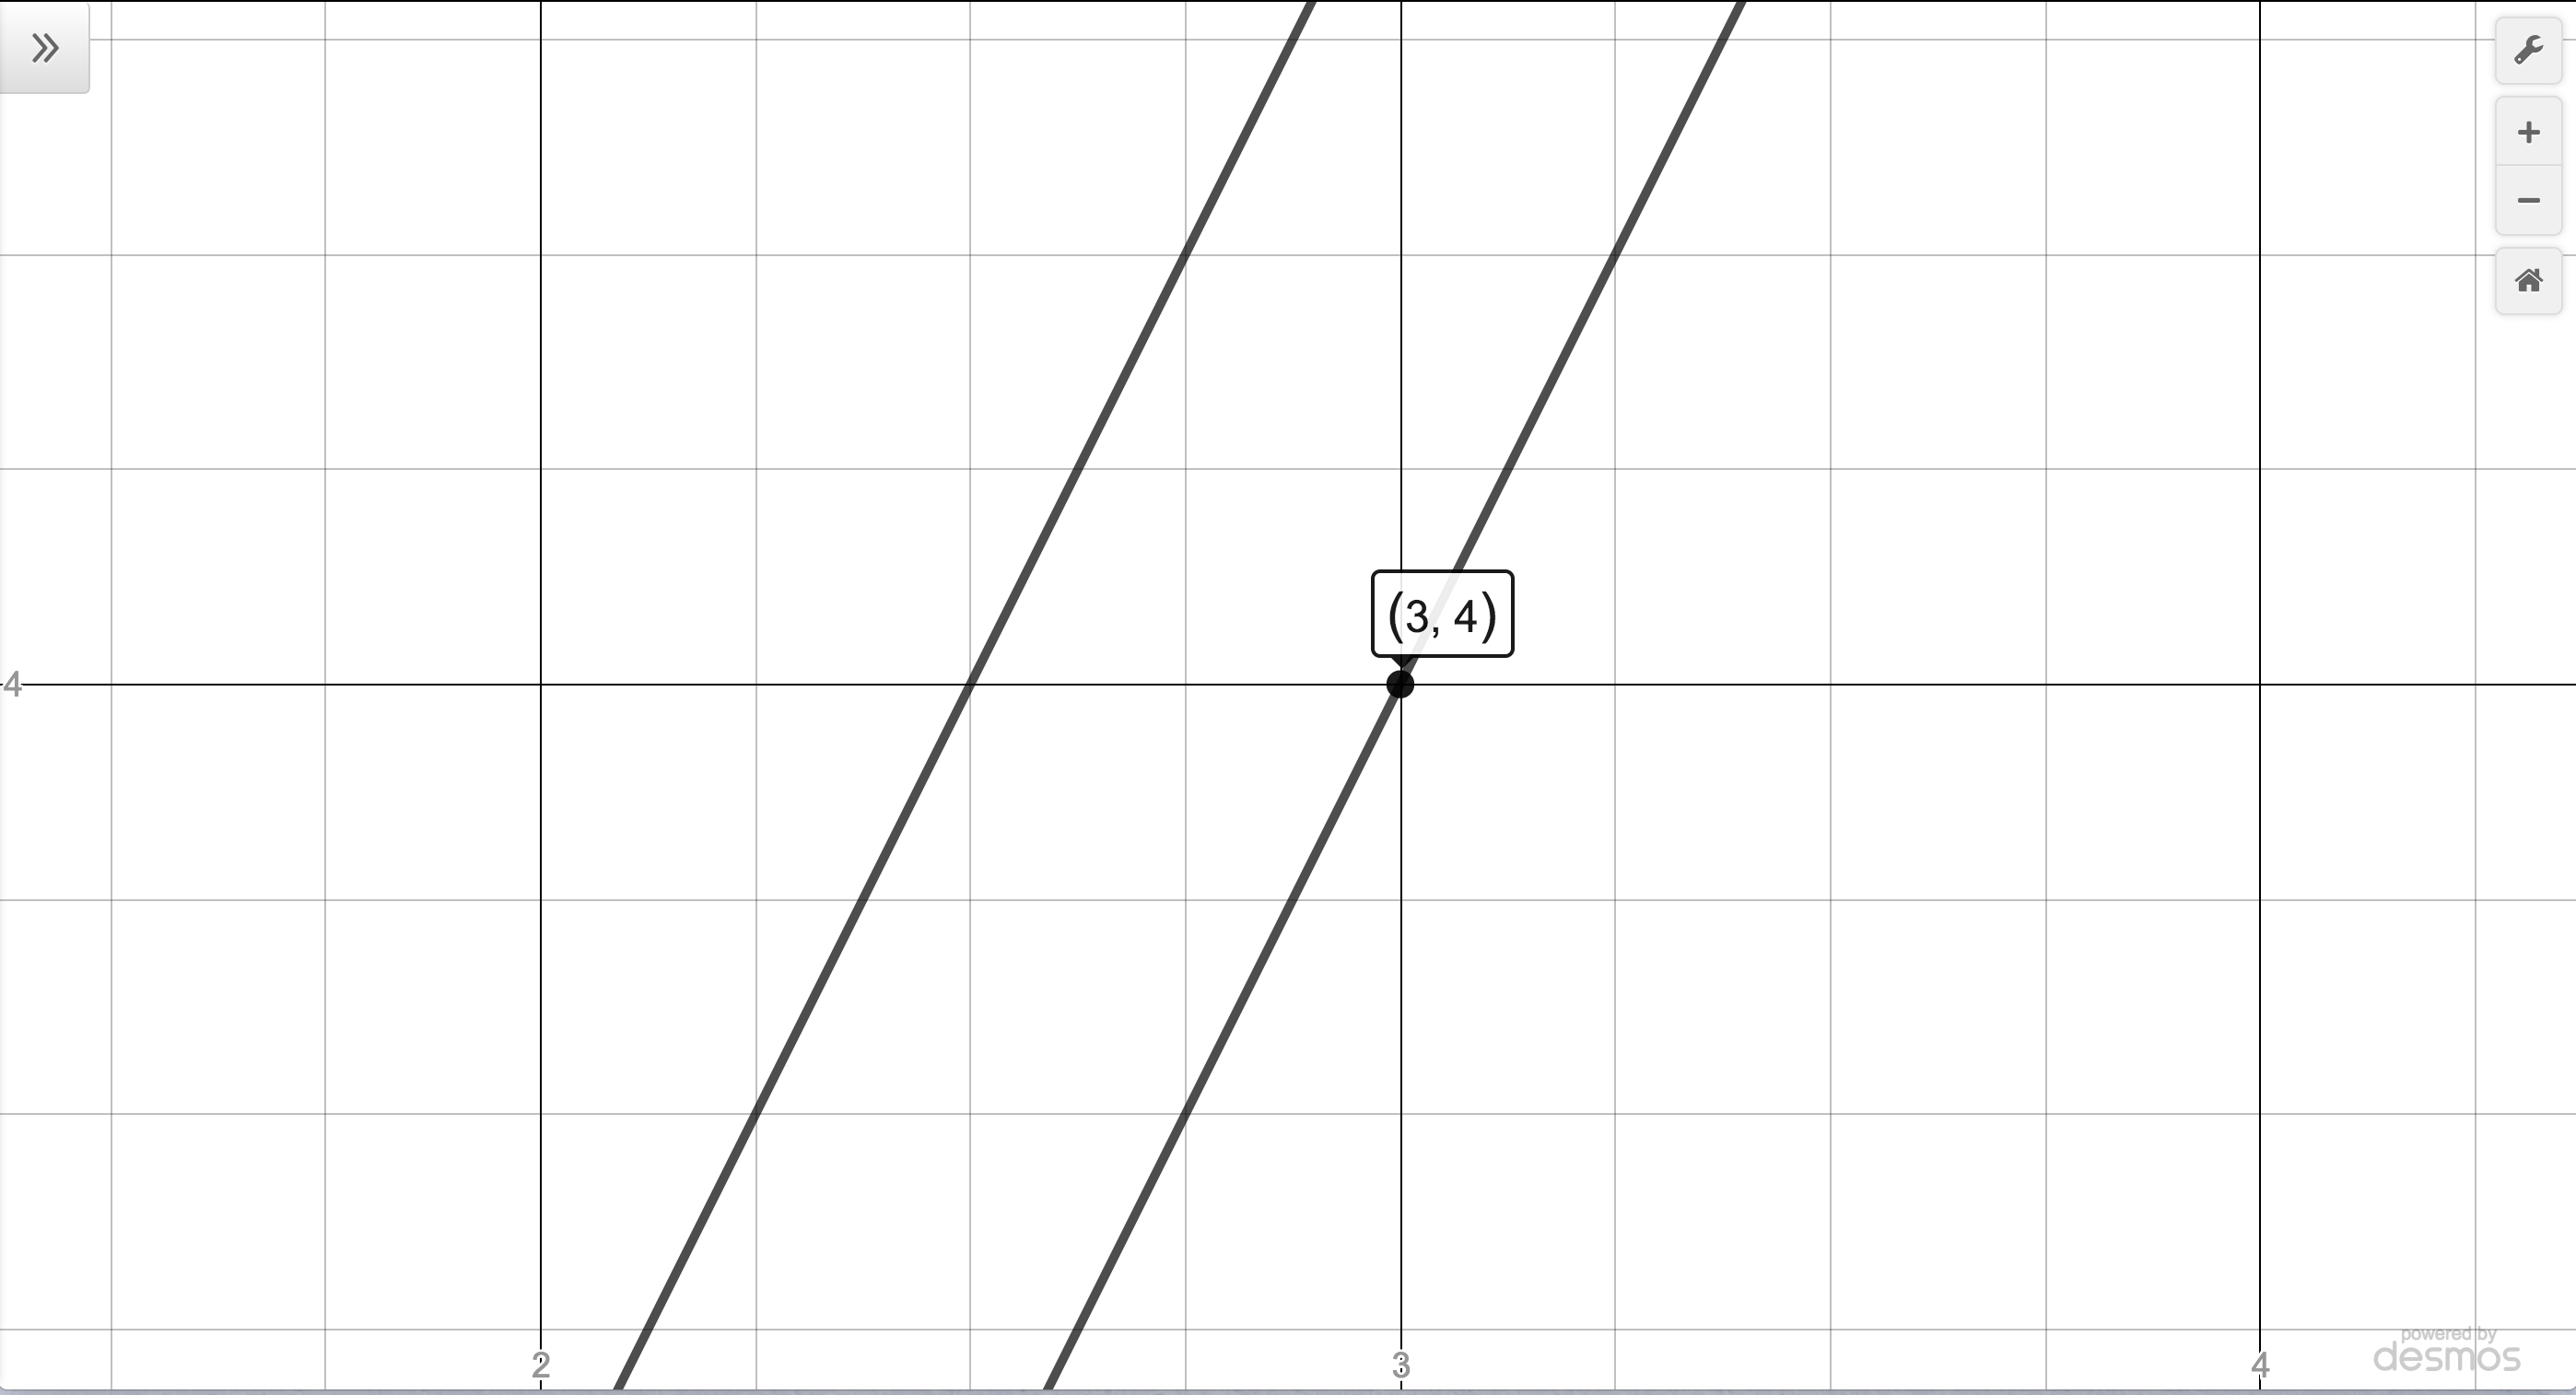
\includegraphics[width=2in]{./AppLinesGraphics/A5Graph01.jpg} &

\hspace{0.75in} 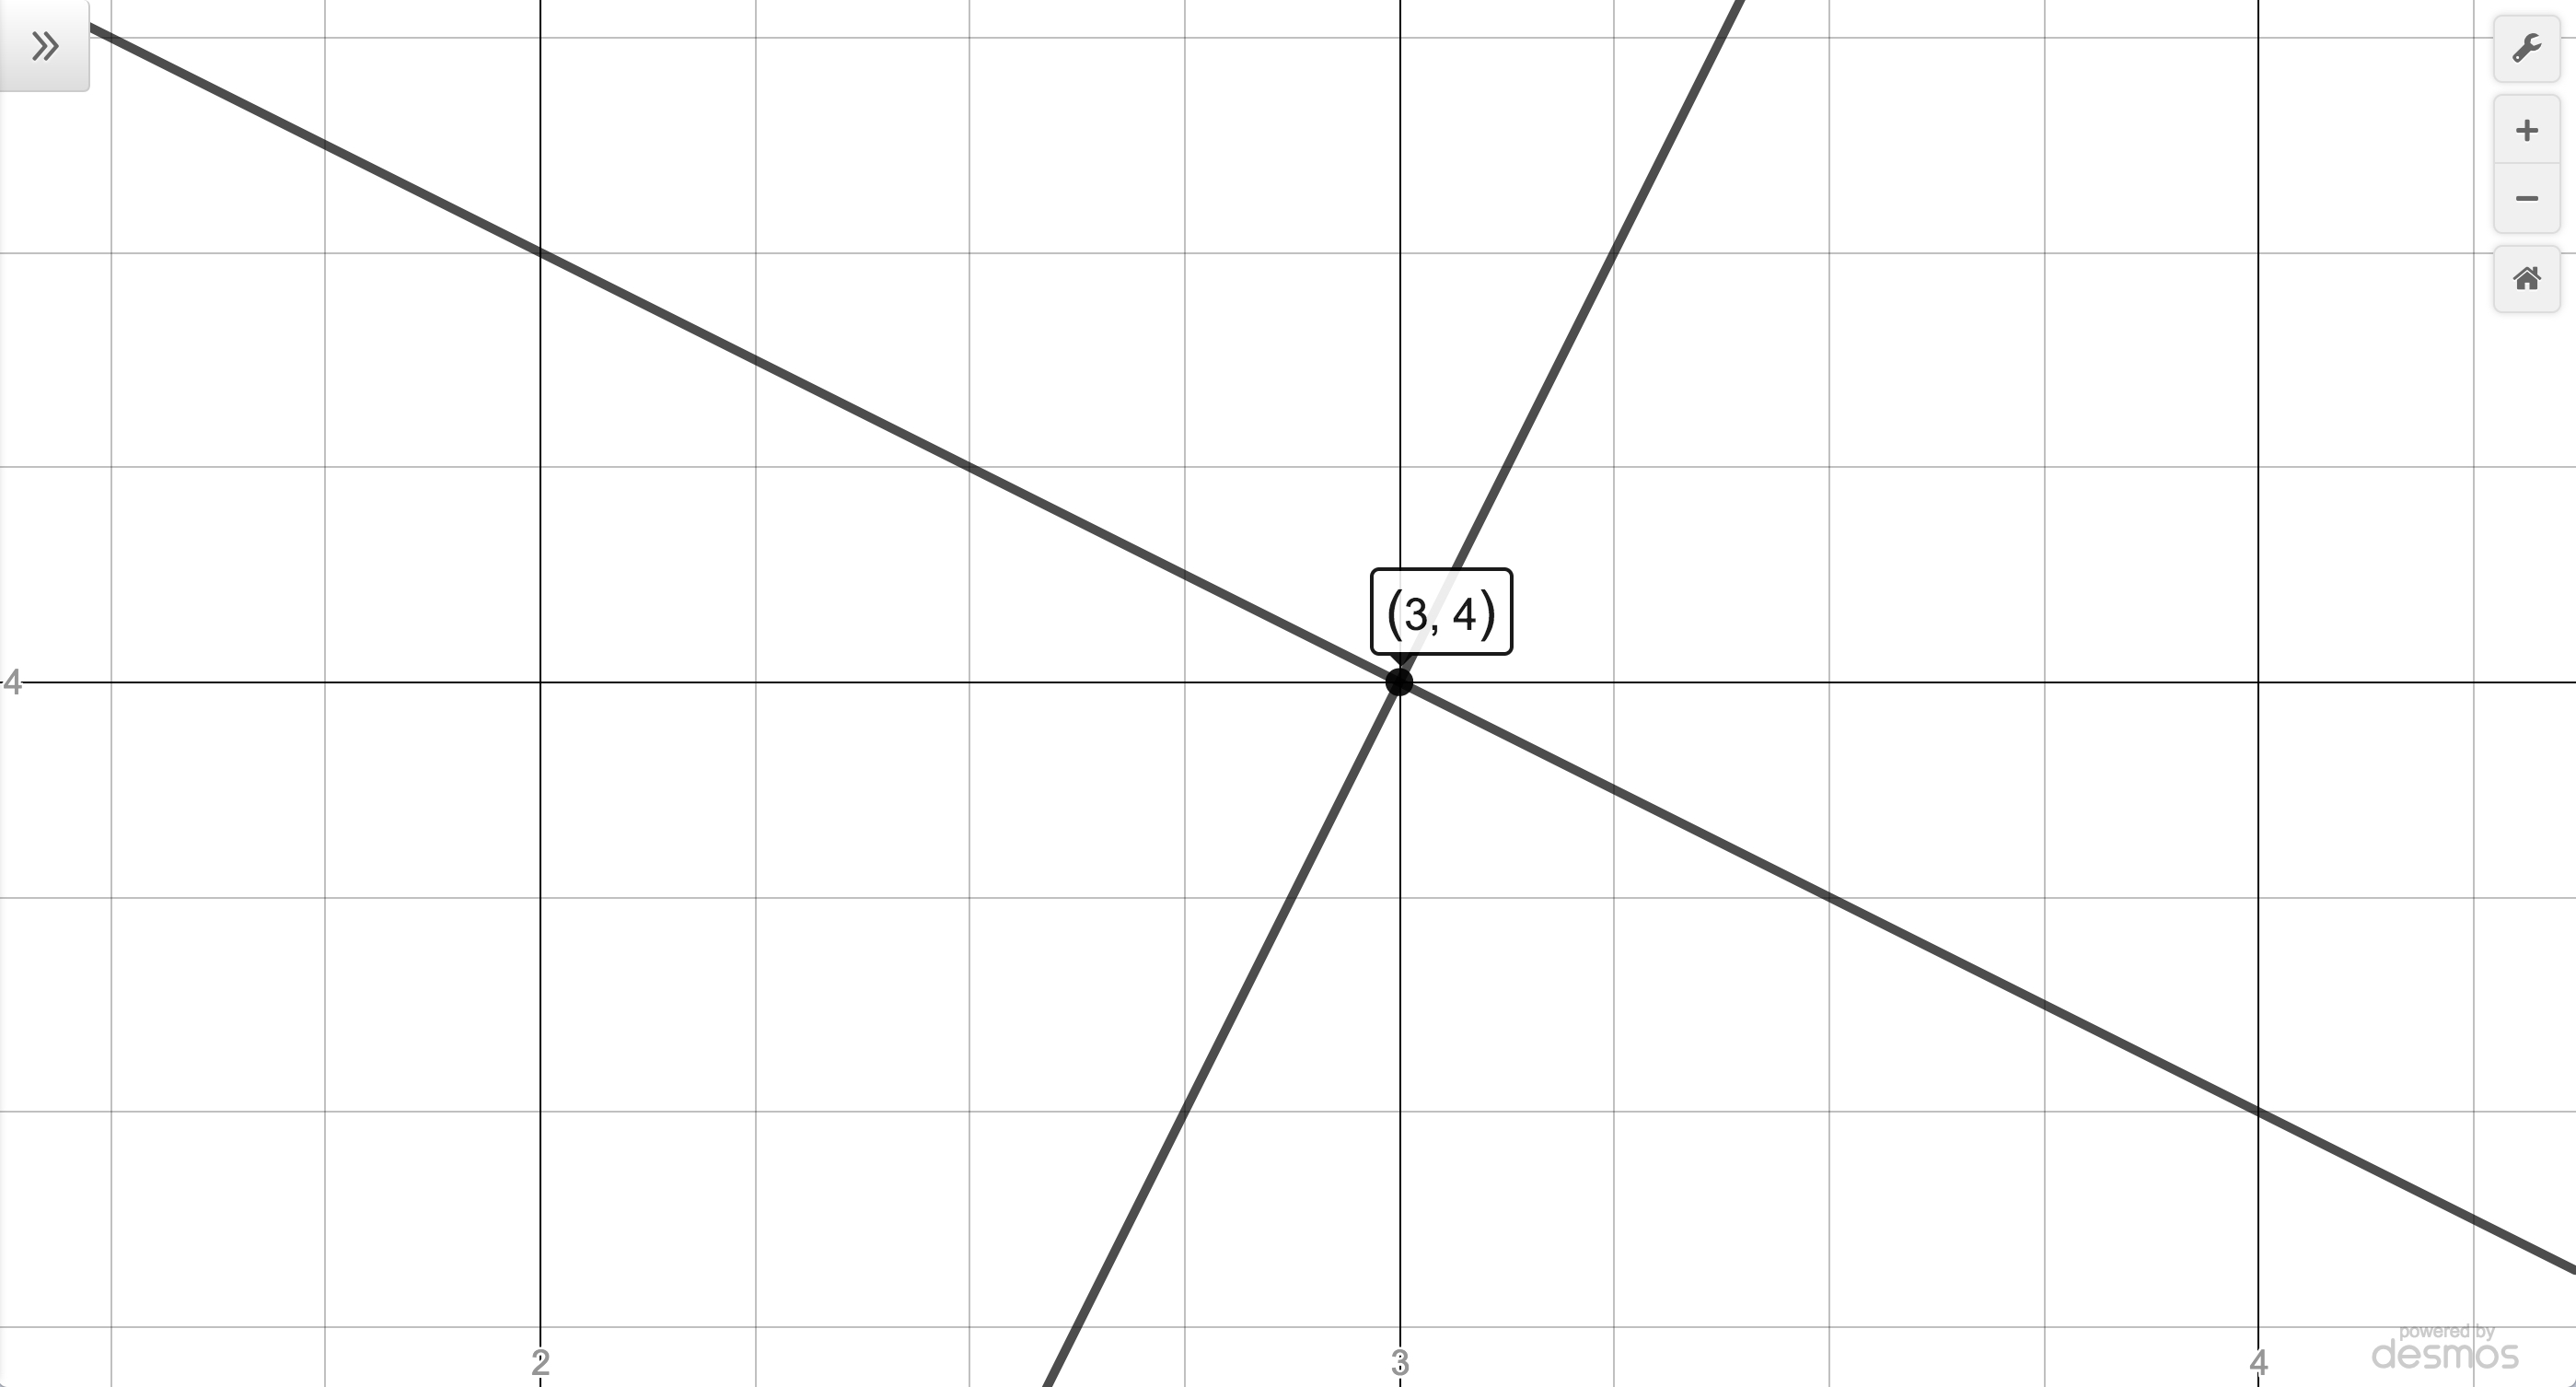
\includegraphics[width=2in]{./AppLinesGraphics/A5Graph02.jpg} \\

$y = 2x-1$ and  & 

 \hspace{0.75in}  $y = 2x-1$ and  \\
 
 \boldmath $y=2x-2$ & \hspace{0.75in} \boldmath $y= -\frac{1}{2} x + \frac{11}{2} $\\
 
\end{tabular}

\end{center}



\end{enumerate}


\end{ex}

\phantomsection

\label{inversemidpoint}

Our last example with lines sets up a fourth kind of symmetry which will be revisited in Section \ref{InverseFunctions}.  

\begin{ex} \label{inversemidpointex2} Show that the points $(a,b)$ and $(b,a)$ in the $xy$-plane are symmetric about the line $y = x$.  

\medskip

{\bf Solution.}  If $a = b$ then $(a, b) = (a, a) = (b, a)$ and this point lies on the line $y = x$.\footnote{Please ask your instructor if lying on the line counts as being `symmetric about the line' or not.}  To prove the claim for the case when $a \neq b$, we will show that the line $y = x$ is a perpendicular bisector of the line segment with endpoints $(a,b)$ and $(b,a)$, as illustrated below.


\begin{center}
\begin{mfpic}[15]{-1}{5}{-1}{5}
\arrow \reverse \arrow \polyline{(-1,-1), (4,4)}
\tlabel[cc](5,-0.5){\scriptsize $x$}
\tlabel[cc](0.5,5){\scriptsize $y$}
\tlabel[cc](1,3.5){\scriptsize $(a,b)$}
\tlabel[cc](3,0.5){\scriptsize $(b,a)$}
\dashed \polyline{(1,3), (3,1)}
\polyline{(2,2), (1.75, 2.25), (2,2.5), (2.25, 2.25)} 
\point[3pt]{(1,3),(3,1), (2,2)}
\tlpointsep{4pt}
\axes

\end{mfpic}


\end{center}



To show the `perpendicular' part,  we first note the slope of the line containing $(a,b)$ and $(b,a)$ is \[ m= \dfrac{a-b}{b-a} = \dfrac{\cancel{(a-b)}}{-\cancel{(b-a)}} = -1\]

Since the slope of $y = x = 1x + 0$ is $m = 1$,  we see that the slopes of these two lines are negative reciprocals.  Hence, $y=x$ and the line segment with endpoints $(a,b)$ and $(b,a)$ are perpendicular.  For the `bisector' part, we \co{use Equation \ref{midpointformula} to}find the midpoint of  the line segment with endpoints $(a,b)$ and $(b,a)$:

\setlength{\extrarowheight}{10pt}

\[ \begin{array}{rcl}

 M & = & \left( \dfrac{a+b}{2},  \dfrac{b+a}{2} \right) \\
   & = & \left( \dfrac{a+b}{2},  \dfrac{a+b}{2} \right)  \\ \end{array} \]

Since the $x$ and $y$ coordinates of this point are the same, we find that the midpoint lies on the line $y=x$. \qed

\end{ex}

\newpage

\subsection{Exercises}

\label{ExercisesforAppLines}

In Exercises \ref{pointslopegivenlinefirst} - \ref{pointslopegivenlinelast}, find both the point-slope form and the slope-intercept form of the line with the given slope which passes through the given point.

\begin{multicols}{2}
\begin{enumerate}

\item $m = 3, \;\; P(3, -1)$ \label{pointslopegivenlinefirst}
\item $m = -2, \;\; P(-5, 8)$

\setcounter{HW}{\value{enumi}}
\end{enumerate}
\end{multicols}

\begin{multicols}{2}
\begin{enumerate}
\setcounter{enumi}{\value{HW}}

\item $m = -1, \;\; P(-7, -1)$
\item $m = \frac{2}{3}, \;\; P(-2, 1)$

\setcounter{HW}{\value{enumi}}
\end{enumerate}
\end{multicols}

\begin{multicols}{2}
\begin{enumerate}
\setcounter{enumi}{\value{HW}}

\item $m = -\frac{1}{5}, \;\; P(10, 4)$
\item $m = \frac{1}{7}, \;\; P(-1, 4)$

\setcounter{HW}{\value{enumi}}
\end{enumerate}
\end{multicols}

\begin{multicols}{2}
\begin{enumerate}
\setcounter{enumi}{\value{HW}}

\item $m = 0, \;\; P(3, 117)$
\item $m = -\sqrt{2}, \;\; P(0, -3)$

\setcounter{HW}{\value{enumi}}
\end{enumerate}
\end{multicols}

\begin{multicols}{2}
\begin{enumerate}
\setcounter{enumi}{\value{HW}}

\item $m = -5, \;\; P(\sqrt{3}, 2\sqrt{3})$
\item $m = 678, \;\; P(-1, -12)$ \label{pointslopegivenlinelast}

\setcounter{HW}{\value{enumi}}
\end{enumerate}
\end{multicols}

In Exercises \ref{twopointsgivenlinefirst} - \ref{twopointsgivenlinelast}, find the slope-intercept form of the line which passes through the given points.

\begin{multicols}{2}
\begin{enumerate}
\setcounter{enumi}{\value{HW}}

\item $P(0, 0), \; Q(-3, 5)$ \label{twopointsgivenlinefirst}
\item $P(-1, -2), \; Q(3, -2)$

\setcounter{HW}{\value{enumi}}
\end{enumerate}
\end{multicols}

\begin{multicols}{2}
\begin{enumerate}
\setcounter{enumi}{\value{HW}}

\item $P(5, 0), \; Q(0, -8)$
\item $P(3, -5), \; Q(7, 4)$

\setcounter{HW}{\value{enumi}}
\end{enumerate}
\end{multicols}

\begin{multicols}{2}
\begin{enumerate}
\setcounter{enumi}{\value{HW}}

\item $P(-1,5), \; Q(7, 5)$
\item $P(4, -8), \; Q(5, -8)$

\setcounter{HW}{\value{enumi}}
\end{enumerate}
\end{multicols}

\begin{multicols}{2}
\begin{enumerate}
\setcounter{enumi}{\value{HW}}

\item $P\left(\frac{1}{2}, \frac{3}{4} \right), \; Q\left(\frac{5}{2}, -\frac{7}{4} \right)$
\item $P\left(\frac{2}{3}, \frac{7}{2} \right), \; Q\left(-\frac{1}{3}, \frac{3}{2} \right)$

\setcounter{HW}{\value{enumi}}
\end{enumerate}
\end{multicols}

\begin{multicols}{2}
\begin{enumerate}
\setcounter{enumi}{\value{HW}}

\item $P\left(\sqrt{2}, -\sqrt{2} \right), \; Q\left(-\sqrt{2}, \sqrt{2} \right)$
\item $P\left(-\sqrt{3}, -1 \right), \; Q\left(\sqrt{3}, 1 \right)$ \label{twopointsgivenlinelast}

\setcounter{HW}{\value{enumi}}
\end{enumerate}
\end{multicols}

In Exercises \ref{graphlineexerfirst} - \ref{graphlineexerlast}, graph the line.  Find the slope, $y$-intercept and $x$-intercept, if any exist.

\begin{multicols}{2}
\begin{enumerate}
\setcounter{enumi}{\value{HW}}

\item $y = 2x - 1$ \label{graphlineexerfirst}
\item $y = 3 - x$

\setcounter{HW}{\value{enumi}}
\end{enumerate}
\end{multicols}

\begin{multicols}{2}
\begin{enumerate}
\setcounter{enumi}{\value{HW}}

\item $y = 3$
\item $y = 0$

\setcounter{HW}{\value{enumi}}
\end{enumerate}
\end{multicols}

\begin{multicols}{2}
\begin{enumerate}
\setcounter{enumi}{\value{HW}}

\item $y = \frac{2}{3} x + \frac{1}{3}$ \vphantom{$\dfrac{1-x}{2}$}
\item $y = \dfrac{1-x}{2}$ \label{graphlineexerlast}

\setcounter{HW}{\value{enumi}}
\end{enumerate}
\end{multicols}




\begin{enumerate}
\setcounter{enumi}{\value{HW}}

\item  Graph $3v + 2w = 6$ on both the $vw$- and $wv$-axes.  What characteristics to both graphs share?  What's different?

\item  Find all of the points on the line $y=2x+1$ which are $4$ units from the point $(-1,3)$.

\setcounter{HW}{\value{enumi}}
\end{enumerate}

In Exercises \ref{parallelfirst} - \ref{parallellast}, you are given a line and a point which is not on that line.  Find the line parallel to the given line which passes through the given point.


\begin{multicols}{2}
\begin{enumerate}
\setcounter{enumi}{\value{HW}}

\item $y = 3x + 2, \; P(0, 0)$ \label{parallelfirst}
\item $y = -6x + 5, \; P(3, 2)$

\setcounter{HW}{\value{enumi}}
\end{enumerate}
\end{multicols}


\begin{multicols}{2}
\begin{enumerate}
\setcounter{enumi}{\value{HW}}

\item $y = \frac{2}{3} x - 7, \; P(6, 0)$
\item $y = \dfrac{4-x}{3}, \; P(1, -1)$


\setcounter{HW}{\value{enumi}}
\end{enumerate}
\end{multicols}


\begin{multicols}{2}
\begin{enumerate}
\setcounter{enumi}{\value{HW}}

\item $y = 6, \; P(3, -2)$
\item $x=1, \; P(-5,0)$ \label{parallellast}


\setcounter{HW}{\value{enumi}}
\end{enumerate}
\end{multicols}


\phantomsection
\label{perpendicularlines}

In Exercises \ref{perpendlinefirst} - \ref{perpendlinelast}, you are given a line and a point which is not on that line.  Find the line perpendicular to the given line which passes through the given point.

\begin{multicols}{2}
\begin{enumerate}
\setcounter{enumi}{\value{HW}}


\item $y = \frac{1}{3}x + 2, \; P(0, 0)$ \label{perpendlinefirst}
\item $y = -6x + 5, \; P(3, 2)$

\setcounter{HW}{\value{enumi}}
\end{enumerate}
\end{multicols}

\begin{multicols}{2}
\begin{enumerate}
\setcounter{enumi}{\value{HW}}

\item $y = \frac{2}{3} x - 7, \; P(6, 0)$
\item $y = \dfrac{4-x}{3}, \; P(1, -1)$


\setcounter{HW}{\value{enumi}}
\end{enumerate}
\end{multicols}

\begin{multicols}{2}
\begin{enumerate}
\setcounter{enumi}{\value{HW}}

\item $y = 6, \; P(3, -2)$
\item $x=1, \; P(-5,0)$ \label{perpendlinelast}


\setcounter{HW}{\value{enumi}}
\end{enumerate}
\end{multicols}


\begin{enumerate}
\setcounter{enumi}{\value{HW}}

\item We shall now prove that $y = m_{\mbox{\tiny$1$}}x + b_{\mbox{\tiny$1$}}$ is perpendicular to $y = m_{\mbox{\tiny$2$}}x + b_{\mbox{\tiny$2$}}$ if and only if $m_{\mbox{\tiny$1$}} \cdot m_{\mbox{\tiny$2$}} = -1$.  To make our lives easier we shall assume that $m_{\mbox{\tiny$1$}} > 0$ and $m_{\mbox{\tiny$2$}} < 0$.  We can also ``move'' the lines so that their point of intersection is the origin without messing things up, so we'll assume $b_{\mbox{\tiny$1$}} = b_{\mbox{\tiny$2$}} = 0.$  (Take a moment with your classmates to discuss why this is okay.)  Graphing the lines and plotting the points $O(0, 0)\;$, $P(1, m_{\mbox{\tiny$1$}})\;$ and $Q(1, m_{\mbox{\tiny$2$}})$ gives us the following set up. \label{perpendicularlineproof}

\begin{center}

\begin{mfpic}[18]{-5}{5}{-5}{5}
\point[3pt]{(0, 0), (1.5, 0.75), (1.5, -3)}
\arrow \reverse \arrow \polyline{( -4, -2), (4, 2)}
\arrow \reverse \arrow \polyline{( -2, 4), (2, -4)}
\polyline{(1.5, 0.75), (1.5, -3)}
\tlabel(1.2, 1){\scriptsize $P$}
\tlabel(-.5,-.6){\scriptsize $O$}
\tlabel(1.2,-3.55){\scriptsize $Q$}
\axes
\tlabel[cc](5,-0.5){\scriptsize $x$}
\tlabel[cc](0.5,5){\scriptsize $y$}
\end{mfpic}

\end{center}

The line $y = m_{\mbox{\tiny$1$}}x$ will be perpendicular to the line $y = m_{\mbox{\tiny$2$}}x$ if and only if $\bigtriangleup OPQ$ is a right triangle.  Let $d_{\mbox{\tiny$1$}}$ be the distance from $O$ to $P$, let $d_{\mbox{\tiny$2$}}$ be the distance from $O$ to $Q$ and let $d_{\mbox{\tiny$3$}}$ be the distance from $P$ to $Q$.  Use the Pythagorean Theorem to show that $\bigtriangleup OPQ$ is a right triangle if and only if $m_{\mbox{\tiny$1$}} \cdot m_{\mbox{\tiny$2$}} = -1$ by showing $d_{\mbox{\tiny$1$}}^{2} + d_{\mbox{\tiny$2$}}^{2} = d_{\mbox{\tiny$3$}}^2$ if and only if $m_{\mbox{\tiny$1$}} \cdot m_{\mbox{\tiny$2$}} = -1$.  


\end{enumerate}

\newpage

\subsection{Answers}

\begin{multicols}{2}
\begin{enumerate}

\item $y+1 = 3(x-3)$ \\ $y = 3x-10$
\item $y-8 = -2(x+5)$ \\ $y = -2x-2$

\setcounter{HW}{\value{enumi}}
\end{enumerate}
\end{multicols}

\begin{multicols}{2}
\begin{enumerate}
\setcounter{enumi}{\value{HW}}

\item $y + 1 = -(x+7)$ \\ $y = -x-8$
\item $y - 1 = \frac{2}{3} (x+2)$ \\ $y = \frac{2}{3} x + \frac{7}{3}$

\setcounter{HW}{\value{enumi}}
\end{enumerate}
\end{multicols}

\begin{multicols}{2}
\begin{enumerate}
\setcounter{enumi}{\value{HW}}

\item $y - 4 = -\frac{1}{5} (x-10)$ \\ $y = -\frac{1}{5} x + 6$
\item $y - 4 = \frac{1}{7}(x + 1)$ \\ $y = \frac{1}{7}x + \frac{29}{7}$


\setcounter{HW}{\value{enumi}}
\end{enumerate}
\end{multicols}

\begin{multicols}{2}
\begin{enumerate}
\setcounter{enumi}{\value{HW}}

\item $y - 117 = 0$ \\ $y = 117$
\item $y + 3 = -\sqrt{2}(x - 0)$ \\ $y = -\sqrt{2}x - 3$

\setcounter{HW}{\value{enumi}}
\end{enumerate}
\end{multicols}



\begin{multicols}{2}
\begin{enumerate}
\setcounter{enumi}{\value{HW}}

\item $y - 2\sqrt{3} = -5(x - \sqrt{3})$ \\ $y = -5x + 7\sqrt{3}$ 
\item $y + 12 = 678(x + 1)$ \\ $y = 678x + 666$

\setcounter{HW}{\value{enumi}}
\end{enumerate}
\end{multicols}


\begin{multicols}{2}
\begin{enumerate}
\setcounter{enumi}{\value{HW}}

\item $y = -\frac{5}{3}x$
\item $y = -2$

\setcounter{HW}{\value{enumi}}
\end{enumerate}
\end{multicols}


\begin{multicols}{2}
\begin{enumerate}
\setcounter{enumi}{\value{HW}}

\item $y = \frac{8}{5}x - 8$ 
\item $y = \frac{9}{4}x - \frac{47}{4}$

\setcounter{HW}{\value{enumi}}
\end{enumerate}
\end{multicols}


\begin{multicols}{2}
\begin{enumerate}
\setcounter{enumi}{\value{HW}}

\item $y = 5$
\item $y = -8$

\setcounter{HW}{\value{enumi}}
\end{enumerate}
\end{multicols}

\begin{multicols}{2}
\begin{enumerate}
\setcounter{enumi}{\value{HW}}

\item $y = -\frac{5}{4} x + \frac{11}{8}$ 
\item $y = 2x + \frac{13}{6}$ 

\setcounter{HW}{\value{enumi}}
\end{enumerate}
\end{multicols}

\begin{multicols}{2}
\begin{enumerate}
\setcounter{enumi}{\value{HW}}

\item $y = -x$
\item $y = \frac{\sqrt{3}}{3} x$

\setcounter{HW}{\value{enumi}}
\end{enumerate}
\end{multicols}


\begin{enumerate}
\setcounter{enumi}{\value{HW}}

\item \begin{multicols}{2} \raggedcolumns 

$y =2x-1$

slope: $m = 2$ 

$y$-intercept:  $(0,-1)$

$x$-intercept: $\left(\frac{1}{2}, 0 \right)$ 

\vfill

\columnbreak

\begin{mfpic}[15]{-3}{3}{-4}{4}
\point[3pt]{(0,-1), (0.5,0)}
\axes
\tlabel[cc](3,-0.5){\scriptsize $x$}
\tlabel[cc](0.5,4){\scriptsize $y$}
\xmarks{-2,-1,1,2}
\ymarks{-3,-2,-1,1,2,3}
\tlpointsep{4pt}
\tiny 
\axislabels {x}{{$-2 \hspace{6pt}$} -2,{$-1 \hspace{6pt}$} -1, {$1$} 1, {$2$} 2}
\axislabels {y}{{$-3$} -3,{$-2$} -2,{$-1$} -1, {$1$} 1, {$2$} 2, {$3$} 3}
\normalsize
\arrow \reverse \arrow \function{-1,2, 0.1}{2*x-1}
\end{mfpic}

\end{multicols}

\item \begin{multicols}{2} \raggedcolumns 

$y =3-x$

slope: $m = -1$ 

$y$-intercept:  $(0,3)$

$x$-intercept: $(3, 0)$ 

\vfill

\columnbreak

\begin{mfpic}[15]{-2}{5}{-2}{5}
\point[3pt]{(0,3), (3,0)}
\axes
\tlabel[cc](5,-0.5){\scriptsize $x$}
\tlabel[cc](0.5,5){\scriptsize $y$}
\xmarks{-1,1,2,3,4}
\ymarks{-1,1,2,3,4}
\tlpointsep{4pt}
\tiny 
\axislabels {x}{{$-1 \hspace{6pt}$} -1, {$1$} 1, {$2$} 2, {$3$} 3, {$4$} 4}
\axislabels {y}{{$-1$} -1, {$1$} 1, {$2$} 2, {$3$} 3, {$4$} 4}
\normalsize
\arrow \reverse \arrow \function{-1,4, 0.1}{3-x}
\end{mfpic}

\end{multicols}


\item \begin{multicols}{2} \raggedcolumns 

$y = 3$

slope: $m =0$ 

$y$-intercept:  $(0,3)$

$x$-intercept: none

\vfill

\columnbreak

\begin{mfpic}[15]{-3}{3}{-1}{5}
\point[3pt]{(0,3)}
\axes
\tlabel[cc](3,-0.5){\scriptsize $x$}
\tlabel[cc](0.5,5){\scriptsize $y$}
\xmarks{-2,-1,1,2}
\ymarks{1,2,3,4}
\tlpointsep{4pt}
\tiny 
\axislabels {x}{{$-2 \hspace{6pt}$} -2,{$-1 \hspace{6pt}$} -1, {$1$} 1, {$2$} 2}
\axislabels {y}{{$1$} 1, {$2$} 2, {$3$} 3, {$4$} 4}
\normalsize
\arrow \reverse \arrow \function{-3,3, 0.1}{3}
\end{mfpic}

\end{multicols}

\item \begin{multicols}{2} \raggedcolumns 

$y = 0$

slope: $m =0$ 

$y$-intercept:  $(0,0)$

$x$-intercept: $\{ (x,0) \, | \, \text{$x$ is a real number} \}$

\vfill

\columnbreak

\begin{mfpic}[15]{-3}{3}{-2}{2}

\arrow \polyline{(0,-2), (0,2)}
\tlabel[cc](3,-0.5){\scriptsize $x$}
\tlabel[cc](0.5,2){\scriptsize $y$}
\xmarks{-2,-1,1,2}
\ymarks{-1,1}
\tlpointsep{4pt}
\tiny 
\axislabels {x}{{$-2 \hspace{6pt}$} -2,{$-1 \hspace{6pt}$} -1, {$1$} 1, {$2$} 2}
\axislabels {y}{{$-1$} -1,{$1$} 1}
\normalsize
\penwd{1.15pt}
\arrow \reverse \arrow \function{-3,3, 0.1}{0}
\end{mfpic}

\end{multicols}


\item \begin{multicols}{2} \raggedcolumns 

$y = \frac{2}{3} x + \frac{1}{3}$

slope: $m = \frac{2}{3}$ 

$y$-intercept:  $\left(0, \frac{1}{3}\right)$

$x$-intercept:  $\left(-\frac{1}{2}, 0\right)$

\vfill

\columnbreak

\begin{mfpic}[15]{-3}{3}{-2}{3}
\point[3pt]{(0,0.33333), (-0.5,0)}
\axes
\tlabel[cc](3,-0.5){\scriptsize $x$}
\tlabel[cc](0.5,3){\scriptsize $y$}
\xmarks{-2,-1,1,2}
\ymarks{-1,1,2}
\tlpointsep{4pt}
\tiny 
\axislabels {x}{{$-2 \hspace{6pt}$} -2, {$1$} 1, {$2$} 2}
\axislabels {y}{{$-1$} -1, {$1$} 1, {$2$} 2}
\normalsize
\arrow \reverse \arrow \function{-3,3, 0.1}{0.66667*x+0.33333}
\end{mfpic}

\end{multicols}

\item \begin{multicols}{2} \raggedcolumns 

$y = \dfrac{1-x}{2}$

slope: $m = -\frac{1}{2}$ 

$y$-intercept:  $\left(0, \frac{1}{2}\right)$

$x$-intercept:  $\left(1, 0\right)$

\vfill

\columnbreak

\begin{mfpic}[15]{-3}{3}{-2}{3}
\point[3pt]{(0,0.5), (1,0)}
\axes
\tlabel[cc](3,-0.5){\scriptsize $x$}
\tlabel[cc](0.5,3){\scriptsize $y$}
\xmarks{-2,-1,1,2}
\ymarks{-1,1,2}
\tlpointsep{4pt}
\tiny 
\axislabels {x}{{$-2 \hspace{6pt}$} -2,{$-1 \hspace{6pt}$} -1, {$1$} 1, {$2$} 2}
\axislabels {y}{{$-1$} -1, {$1$} 1, {$2$} 2}
\normalsize
\arrow \reverse \arrow \function{-3,3, 0.1}{0.5-0.5*x}
\end{mfpic}

\end{multicols}

\setcounter{HW}{\value{enumi}}
\end{enumerate}


\begin{enumerate}
\setcounter{enumi}{\value{HW}}

\item  \begin{multicols}{2} \raggedcolumns 

$w = -\frac{3}{2} v + 3$

slope: $m = -\frac{3}{2}$ 

$w$-intercept:  $\left(0, 3\right)$

$v$-intercept:  $\left(2, 0\right)$

\vfill

\columnbreak

\begin{mfpic}[15]{-1}{4}{-1}{4}
\point[3pt]{(0,3), (2,0)}
\axes
\tlabel[cc](4,-0.5){\scriptsize $v$}
\tlabel[cc](0.5,4){\scriptsize $w$}
\xmarks{1,2,3}
\ymarks{1,2,3}
\tlpointsep{4pt}
\tiny 
\axislabels {x}{{$1$} 1, {$2$} 2, {$3$} 3}
\axislabels {y}{{$1$} 1, {$2$} 2, , {$3$} 3}
\normalsize
\arrow \reverse \arrow \polyline{(-0.5, 3.75), (2.5, -0.75)}
\end{mfpic}

\end{multicols}


\begin{multicols}{2} \raggedcolumns 

$v = -\frac{2}{3} w + 2$

slope: $m = -\frac{2}{3}$ 

$v$-intercept:  $\left(0,2 \right)$

$w$-intercept:  $\left(3,0\right)$



\vfill

\columnbreak

\begin{mfpic}[15]{-1}{4}{-1}{4}
\point[3pt]{(0,2), (3,0)}
\axes
\tlabel[cc](4,-0.5){\scriptsize $w$}
\tlabel[cc](0.5,4){\scriptsize $v$}
\xmarks{1,2,3}
\ymarks{1,2,3}
\tlpointsep{4pt}
\tiny 
\axislabels {x}{{$1$} 1, {$2$} 2, {$3$} 3}
\axislabels {y}{{$1$} 1, {$2$} 2, , {$3$} 3}
\normalsize
\arrow \reverse \arrow \polyline{(3.75, -0.5), (-0.75, 2.5)}
\end{mfpic}
 
\end{multicols}

\item $(-1,-1)$ and $\left(\frac{11}{5}, \frac{27}{5}\right)$

\setcounter{HW}{\value{enumi}}
\end{enumerate}

\begin{multicols}{3}
\begin{enumerate}
\setcounter{enumi}{\value{HW}}

\item $y = 3x$
\item $y = -6x + 20$
\item $y = \frac{2}{3} x - 4$


\setcounter{HW}{\value{enumi}}
\end{enumerate}
\end{multicols}

\begin{multicols}{3}
\begin{enumerate}
\setcounter{enumi}{\value{HW}}

\item $y = -\frac{1}{3} x - \frac{2}{3}$
\item $y=-2$
\item $x=-5$


\setcounter{HW}{\value{enumi}}
\end{enumerate}
\end{multicols}


\begin{multicols}{3}
\begin{enumerate}
\setcounter{enumi}{\value{HW}}

\item $y = -3x$
\item $y = \frac{1}{6}x + \frac{3}{2}$
\item $y = -\frac{3}{2} x +9$



\setcounter{HW}{\value{enumi}}
\end{enumerate}
\end{multicols}

\begin{multicols}{3}
\begin{enumerate}
\setcounter{enumi}{\value{HW}}

\item $y = 3x-4$
\item $x=3$
\item $y=0$


\setcounter{HW}{\value{enumi}}
\end{enumerate}
\end{multicols}


\closegraphsfile

\newpage

\section{Systems of Two Linear Equations in Two Unknowns}

\mfpicnumber{1}

\opengraphsfile{AppLinearSystems}

\setcounter{footnote}{0}

\label{AppLinearSystems}

\setlength{\extrarowheight}{0pt}

This section of the Appendix combines ideas from Section \ref{AppLinearEqIneq} and \ref{AppLines} so that we can start to solve systems of linear equations.  Before we get ahead of ourselves, let's review a few definitions.

\medskip

\colorbox{ResultColor}{\bbm

\begin{defn}  \label{lineareqntwovariables}  A \index{equation ! linear of two variables}\index{linear equation ! two variables}\textbf{linear equation in two variables} is an equation of the form $a_{\mbox{\tiny$1$}} x + a_{\mbox{\tiny$2$}} y = c$ where $a_{\mbox{\tiny$1$}}$, $a_{\mbox{\tiny$2$}}$ and $c$ are real numbers and at least one of $a_{\mbox{\tiny$1$}}$ and $a_{\mbox{\tiny$2$}}$ is nonzero.

\end{defn}

\ebm}

\medskip

For reasons which will become clear when you study Chapter \ref{SystemsofEquationsandMatrices}, we are using subscripts in Definition \ref{lineareqntwovariables} to indicate different, but fixed, real numbers and those subscripts have no mathematical meaning beyond that.  For example, $3x - \frac{y}{2} = 0.1$ is a linear equation in two variables with $a_{\mbox{\tiny$1$}} = 3$, $a_{\mbox{\tiny$2$}} = -\frac{1}{2}$ and $c = 0.1$.  We can also consider $x = 5$ to be a linear equation in two variables\footnote{Critics may argue that $x=5$ is clearly an equation in one variable.  It can also be considered an equation in $117$ variables with the coefficients of $116$ variables set to $0$.  As with many conventions in Mathematics, the context will clarify the situation.} by identifying $a_{\mbox{\tiny$1$}} = 1$, $a_{\mbox{\tiny$2$}} = 0$, and $c = 5$.  

\medskip

If $a_{\mbox{\tiny$1$}}$ and $a_{\mbox{\tiny$2$}}$ are both $0$, then depending on $c$, we get either an equation which is \textit{always} true, called an \index{equation ! identity}\index{identity ! statement which is always true}\textbf{identity}, or an equation which is \textit{never} true, called a \index{equation ! contradiction}\index{contradiction}\textbf{contradiction}. (If $c = 0$, then we get $0 = 0$, which is always true.  If $c \neq 0$, then we'd have  $0 \neq 0$, which is never true.)  Even though identities and contradictions have a large role to play throughout Chapter \ref{SystemsofEquationsandMatrices}, we do not consider them linear equations.  The key to identifying linear equations is to note that the variables involved are to the first power and that the coefficients of the variables are numbers.  Some examples of equations which are non-linear are $x^2 + y = 1$, $xy = 5$ and $e^{2x} + \ln(y) = 1$.  The reader should consider why these do not satisfy Definition \ref{lineareqntwovariables}.  

\medskip

We know from our work is Sections \ref{AppLines} that the graphs of linear equations are lines.  If we couple two or more linear equations together, in effect to find the points of intersection of two or more lines, we obtain a \textbf{system of linear equations in two variables}. \index{system of equations ! linear ! two variables} Our first example explores the basic techniques for solving these systems.  Remember - if we are looking for points in the plane, then both the $x$ and $y$ values are important.  This is a key distinction between solving one equation and solving a \emph{system} of equations.

\begin{ex} \label{reviewsubelim}  Solve the following systems of equations.  Check your answer algebraically and graphically.  (Said another way, make sure both $x$ and $y$ are correct!)

\begin{multicols}{3}
\begin{enumerate}

\item  $\left\{ \begin{array}{rcr} 2x - y & = & 1 \\ y & = & 3 \\ \end{array} \right.$ \vphantom{$\left\{ \begin{array}{rcr} \frac{x}{3} -\frac{4y}{5} & = & \frac{7}{5} \\ [3pt] 
\frac{2x}{9} + \frac{y}{3} & = & \frac{1}{2} \\ \end{array} \right.$}

\item  $\left\{ \begin{array}{rcr} 3x+4y & = & -2  \\ -3x-y & = & 5 \\ \end{array} \right.$ \vphantom{$\left\{ \begin{array}{rcr} \frac{x}{3} -\frac{4y}{5} & = & \frac{7}{5}\\[3pt] \frac{2x}{9} + \frac{y}{3} & = & \frac{1}{2} \\ \end{array} \right.$}

\item  $\left\{ \begin{array}{rcr} \frac{x}{3} -\frac{4y}{5} & = & \frac{7}{5} \\ [3pt] 
\frac{2x}{9} + \frac{y}{3} & = & \frac{1}{2} \\ \end{array} \right.$

\setcounter{HW}{\value{enumi}}
\end{enumerate}
\end{multicols}

\begin{multicols}{3}
\begin{enumerate}
\setcounter{enumi}{\value{HW}}

\item  $\left\{ \begin{array}{rcr} 2x - 4y & = & 6 \\ 3x -6y & = & 9\\ \end{array} \right.$ \vphantom{$\left\{ \begin{array}{rcr} x - y & = & 0 \\ x + y & = & 2 \\ -2x + y & = & -2 \end{array} \right.$}

\item  $\left\{ \begin{array}{rcr} 6x + 3y & = & 9 \\ 4x + 2y & = & 12 \\ \end{array} \right.$ \vphantom{$\left\{ \begin{array}{rcr} x - y & = & 0 \\ x + y & = & 2 \\ -2x + y & = & -2 \end{array} \right.$}

\item  $\left\{ \begin{array}{rcr} x - y & = & 0 \\ x + y & = & 2 \\ -2x + y & = & -2 \end{array} \right.$

\end{enumerate}
\end{multicols}

{\bf Solution.}

\begin{enumerate}

\item  Our first system is nearly solved for us.  The second equation tells us that $y=3$.  To find the corresponding value of $x$, we \textbf{substitute} this value for $y$ into the the first equation to obtain $2x -  3 = 1$, so that $x = 2$.  Our solution to the system is $(2,3)$.  To check this algebraically, we substitute $x=2$ and $y=3$ into each equation and see that they are satisfied.  We see $2(2) - 3 = 1$, and $3=3$, as required.  To check our answer graphically, we graph the lines $2x-y = 1$ and $y=3$ and verify that they intersect at $(2,3)$.

\setlength{\extrarowheight}{2pt}

\item  To solve the second system, we use the \textbf{addition} method to \textbf{eliminate} the variable $x$.  We take the two equations as given and `add equals to equals' to obtain \[ \begin{array}{lrcr} & 3x+4y & = & -2  \\ + & (-3x-y  & = & 5 ) \\ \hline & 3y & = & 3\end{array}\] This gives us $y = 1$.  We now substitute $y=1$ into either of the two equations, say $-3x-y = 5$, to get $-3x-1 = 5$ so that $x = -2$.  Our solution is $(-2,1)$.  Substituting $x=-2$ and $y=1$ into the first equation gives $3(-2) + 4(1) = -2$, which is true, and, likewise, when we check $(-2, 1)$ in the second equation, we get $-3(-2) - 1 = 5$, which is also true.  Geometrically, the lines $3x+4y = -2$ and $-3x-y=5$ intersect at $(-2,1)$.

\setlength{\extrarowheight}{0pt}

\begin{center}

\begin{tabular}{m{.5in}m{2in}m{.5in}m{2in}}

$~$

&

\begin{mfpic}[15]{-2}{5}{-2}{5}
\arrow \reverse \arrow \polyline{(-0.5,-2), (3,5)}
\point[3pt]{(2,3)}
\axes
\tlabel[cc](2.5,2.5){\tiny $(2,3)$}
\xmarks{-1,1,2,3,4}
\ymarks{-1,1,2,3,4}
\tlabel(5,-0.5){\scriptsize $x$}
\tlabel(0.5,5){\scriptsize $y$}
\tcaption{\scriptsize \centerline{$2x-y=1$} \\ \centerline{\boldmath $y=3$}}
\tlpointsep{4pt}
\axislabels {x}{{\tiny $-1 \hspace{7pt}$} -1, {\tiny $1$} 1, {\tiny $2$} 2, {\tiny $3$} 3, {\tiny $4$} 4}
\axislabels {y}{{\tiny $1$} 1, {\tiny $2$} 2, {\tiny $4$} 4}
\penwd{1.1pt}
\arrow \reverse \arrow \polyline{(-2,3), (5,3)}
\end{mfpic}

&

$~$
 
&

\begin{mfpic}[15]{-5}{1}{-3}{3}
\arrow \reverse \arrow \polyline{(-4.666,3), (1,-1.25)}
\point[3pt]{(-2,1)}
\axes
\tlabel[cc](-3,0.5){\tiny $(-2,1)$}
\xmarks{-4,-3,-2,-1}
\ymarks{-2,-1,1,2}
\tlabel(1,-0.5){\scriptsize $x$}
\tlabel(0.5,3){\scriptsize $y$}
\tcaption{\scriptsize \centerline{$3x+4y=-2$} \\ \centerline{\boldmath $-3x-y=5$}}
\tlpointsep{4pt}
\axislabels {x}{{\tiny $-4 \hspace{7pt}$} -4,{\tiny $-3 \hspace{7pt}$} -3,{\tiny $-2 \hspace{7pt}$} -2,{\tiny $-1 \hspace{7pt}$} -1}
\axislabels {y}{{\tiny $-2$} -2,{\tiny $-1$} -1,{\tiny $1$} 1, {\tiny $2$} 2}
\penwd{1.1pt}
\arrow \reverse \arrow \polyline{(-2.666,3), (-0.666,-3)}
\end{mfpic}

\\

\end{tabular}

\end{center}

\setlength{\extrarowheight}{2pt} 

\item  The equations in the third system are more approachable if we clear denominators.  We multiply both sides of the first equation by $15$ and both sides of the second equation by $18$ to obtain the kinder, gentler system \[\left\{ \begin{array}{rcr} 5x - 12y & = & 21  \\ 4x  + 6y & = & 9 \\ \end{array} \right.\]  Adding these two equations directly fails to eliminate either of the variables, but we note that if we multiply the first equation by $4$ and the second by $-5$, we will be in a position to eliminate the $x$ term \[ \begin{array}{lrcr} & 20x-48y & = & 84  \\ + & (-20x-30y  & = & -45 ) \\ \hline  & -78y & = & 39\end{array}\] From this we get $y = -\frac{1}{2}$.  We can temporarily avoid too much unpleasantness by choosing to substitute $y = -\frac{1}{2}$ into one of the equivalent equations we found by clearing denominators, say into $5x - 12y  =  21$.  We get $5x + 6 = 21$ which gives $x=3$.  Our answer is $\left(3, -\frac{1}{2}\right)$.  At this point, we have no choice $-$ in order to check an answer algebraically, we must see if the answer satisfies both of the \textit{original} equations, so we substitute $x = 3$ and $y = -\frac{1}{2}$ into both $\frac{x}{3} -\frac{4y}{5} = \frac{7}{5}$ and $\frac{2x}{9} + \frac{y}{3} = \frac{1}{2}$.  We leave it to the reader to verify that the solution is correct.  Graphing both of the lines involved with considerable care yields an intersection point of $\left(3, -\frac{1}{2}\right)$.  (The picture is on the next page.)


\item  An eerie calm settles over us as we cautiously approach our fourth system.  Do its friendly integer coefficients belie something more sinister?  We note that if we multiply both sides of the first equation by $3$ and both sides of the second equation by $-2$, we are ready to eliminate the $x$ \[ \begin{array}{lrcr} & 6x-12y & = & 18  \\ + & (-6x+12y  & = & -18 ) \\ \hline  & 0 & = & 0\end{array}\] We eliminated not only the $x$, but the $y$ as well and we are left with the identity $0=0$.  This means that these two different linear equations are, in fact, equivalent.  In other words, if an ordered pair $(x,y)$ satisfies the equation $2x-4y = 6$, it \textit{automatically} satisfies the equation $3x-6y = 9$.  

\setlength{\extrarowheight}{0pt} 

\medskip

This system has infinitely many solutions and one way to describe the solution set to this system is to use the roster method\footnote{See Section \ref{AppSetTheory} for a review of this.} and write $\{(x,y) \, | \, 2x-4y = 6\}$.  While this is correct (and corresponds exactly to what's happening graphically, as we shall see shortly), we take this opportunity to introduce the notion of a \index{parametric solution} \index{system of equations ! parametric solution}\textbf{parametric solution to a system}.  

\medskip

Our first step is to solve $2x-4y = 6$ for one of the variables, say $y = \frac{1}{2} x - \frac{3}{2}$.  For each value of $x$, the formula $y = \frac{1}{2} x - \frac{3}{2}$ determines the corresponding $y$-value of a solution.  Since we have no restriction on $x$, it is called a \index{system of equations ! free variable}\index{free variable}\textbf{free variable}.  We let $x=t$, a so-called `parameter', and get $y = \frac{1}{2} t - \frac{3}{2}$. Our set of solutions can then be described as $\left\{ \left(t, \frac{1}{2} t - \frac{3}{2}\right) \, | \, -\infty < t < \infty \right\}$.\footnote{Note that we could have just as easily chosen to solve $2x-4y = 6$ for $x$ to obtain $x = 2y + 3$.  Letting $y$ be the parameter $t$, we have that for any value of $t$, $x = 2t+3$, which gives $\{(2t+3, t) \, | \, - \infty < t < \infty\}$.  There is no one correct way to parameterize the solution set, which is why it is always best to check your answer.}  

\medskip

For specific values of $t$, we can generate solutions.  For example, $t=0$ gives us the solution $\left(0,-\frac{3}{2}\right)$;  $t = 117$ gives us $(117,57)$, and while we can  check that each of these particular solutions satisfy both equations, the question is how do we check our general answer algebraically?  Same as always.  

\medskip

We claim that for any real number $t$, the pair $\left(t, \frac{1}{2} t - \frac{3}{2}\right)$ satisfies both equations.  Substituting $x = t$ and $y =  \frac{1}{2} t - \frac{3}{2}$ into $2x - 4y = 6$ gives $2t - 4\left(\frac{1}{2} t - \frac{3}{2}\right) = 6$.  Simplifying, we get $2t - 2t + 6 = 6$, which is always true.  Similarly, when we make these substitutions in the equation $3x-6y = 9$, we get $3t - 6\left(\frac{1}{2} t - \frac{3}{2}\right) = 9$ which reduces to $3t - 3t + 9 = 9$, so it checks out, too.  

\medskip

Geometrically, $2x-4y = 6$ and $3x-6y=9$ are the same line, which means that they intersect at every point on their graphs.  The reader is encouraged to think about how our parametric solution says exactly that.

\pagebreak

The picture for this system is shown below on the right while the picture for the previous example is shown on the left.

\begin{center}

\begin{tabular}{m{.5in}m{2in}m{.5in}m{2in}}

$~$

&

\begin{mfpic}[10]{-2}{8}{-5}{3}
\arrow \reverse \arrow \polyline{(-2,-2.583), (8,1.583)}
\point[3pt]{(3,-0.5)}
\axes
\tlabel[cc](3,-2){\tiny $\left(3,-\frac{1}{2}\right)$}
\xmarks{-1,1,2,3,4,5,6,7}
\ymarks{-4,-3,-2,-1,1,2}
\tlabel(8,-0.5){\scriptsize $x$}
\tlabel(0.5,3){\scriptsize $y$}
\tcaption{\scriptsize \centerline{$\frac{x}{3} -\frac{4y}{5} = \frac{7}{5}$} \\ \centerline{\boldmath $\frac{2x}{9} + \frac{y}{3} = \frac{1}{2}$}}
\tlpointsep{4pt}
\axislabels {x}{{\tiny $-1 \hspace{7pt}$} -1, {\tiny $1$} 1, {\tiny $2$} 2, {\tiny $4$} 4, {\tiny $5$} 5, {\tiny $6$} 6, {\tiny $7$} 7}
\axislabels {y}{{\tiny $-4 \hspace{7pt}$} -4,{\tiny $-3 \hspace{7pt}$} -3,{\tiny $-2 \hspace{7pt}$} -2,{\tiny $-1 \hspace{7pt}$} -1,{\tiny $1$} 1}
\penwd{1.1pt}
\arrow \reverse \arrow \polyline{(-2.25,3), (8,-3.833)}
\end{mfpic}

&

$~$
 
&

\begin{mfpic}[15]{-1}{5}{-3}{3}
\axes
\xmarks{1,2,3,4}
\ymarks{-2,-1,1,2}
\tlabel(5,-0.5){\scriptsize $x$}
\tlabel(0.5,3){\scriptsize $y$}
\tcaption{\scriptsize \centerline{$2x - 4y = 6$} \\ \centerline{\boldmath $3x-6y = 9$} \\ \centerline{(Same line.)}}
\tlpointsep{4pt}
\axislabels {x}{{\tiny $1$} 1,{\tiny $2$} 2,{\tiny $3$} 3,{\tiny $4$} 4}
\axislabels {y}{{\tiny $-1$} -1,{\tiny $1$} 1, {\tiny $2$} 2}
\penwd{1.1pt}
\arrow \reverse \arrow \polyline{(-1,-2), (5,1)}
\end{mfpic}

\\

\end{tabular}

\end{center}

\item  Multiplying both sides of the first equation by $2$ and the both sides of the second equation by $-3$, we set the stage to eliminate $x$ 

\setlength{\extrarowheight}{2pt}
\[ \begin{array}{lrcr} & 12x + 6y & = & 18  \\ + & (-12x-6y  & = & -36 ) \\ \hline  & 0 & = & -18 \end{array}\] 
\setlength{\extrarowheight}{0pt}

As in the previous example, both $x$ and $y$ dropped out of the equation, but we are left with an irrevocable contradiction, $0 = -18$. This tells us that it is impossible to find a pair $(x,y)$ which satisfies both equations; in other words, the system has no solution.  Graphically, the lines  $6x + 3y =9$ and  $4x + 2y = 12$ are distinct and parallel, so they do not intersect.

\item  We can begin to solve our last system by adding the first two equations  

\setlength{\extrarowheight}{2pt}
\[ \begin{array}{lrcr} & x - y & = & 0  \\ + & (x + y & = & 2 ) \\ \hline  & 2x & = & 2 \end{array}\]  
\setlength{\extrarowheight}{0pt}

which gives $x = 1$.  Substituting this into the first equation gives $1 - y = 0$ so that $y = 1$.  We seem to have determined a solution to our system, $(1,1)$.  While this checks in the first two equations, when we substitute $x=1$ and $y=1$ into the third equation, we get $-2(1) + (1) = -2$ which simplifies to the contradiction $-1 = -2$.  Graphing the lines $x-y=0$, $x+y = 2$, and $-2x+y=-2$, we see that the first two lines do, in fact, intersect at $(1,1)$, however, all three lines never intersect at the same point simultaneously, which is what is required if a solution to the system is to be found.

\begin{center}

\begin{tabular}{m{.5in}m{2in}m{.5in}m{2in}}

$~$

&

\begin{mfpic}[15][7]{-1}{4}{-4}{7}
\arrow \reverse \arrow \polyline{(-1,5), (3.5,-4)}
\axes
\xmarks{1,2,3}
\ymarks{-3,-2,-1,1,2,3,4,5,6}
\tlabel(4,-0.5){\scriptsize $x$}
\tlabel(0.5,7){\scriptsize $y$}
\tcaption{\scriptsize \centerline{$6x + 3y =9$} \\ \centerline{\boldmath $4x + 2y = 12$}}
\tlpointsep{4pt}
\axislabels {x}{{\tiny $1$} 1, {\tiny $2$} 2}
\axislabels {y}{{\tiny $-3 \hspace{7pt}$} -3,{\tiny $-2 \hspace{7pt}$} -2,{\tiny $-1 \hspace{7pt}$} -1,{\tiny $1$} 1,{\tiny $2$} 2,{\tiny $3$} 3,{\tiny $4$} 4,{\tiny $5$} 5,{\tiny $6$} 6}
\penwd{1.1pt}
\arrow \reverse \arrow \polyline{(-0.5,7), (4,-2)}
\end{mfpic}

&

$~$
 
&

\begin{mfpic}[15]{-1}{3}{-3}{3}
\axes
\xmarks{1,2}
\ymarks{-2,-1,1,2}
\tlabel(3,-0.5){\scriptsize $x$}
\tlabel(0.5,3){\scriptsize $y$}
\tcaption{\scriptsize \centerline{$y-x = 0$} \\ \centerline{$y+x = 2$} \\ \centerline{$-2x+y=-2$}}
\tlpointsep{4pt}
\axislabels {y}{{\tiny $-1$} -1,{\tiny $1$} 1}
\arrow \reverse \arrow \polyline{(-1,-1), (3,3)}
\arrow \reverse \arrow \polyline{(-1,3), (3,-1)}
\arrow \reverse \arrow \polyline{(-0.5,-3), (2.5,3)}
\end{mfpic} \\

\end{tabular}

\end{center}

\vspace{-.25in} \qed

\end{enumerate}

\end{ex}

A few remarks about Example \ref{reviewsubelim} are in order.  Notice that some of the systems of linear equations had solutions while others did not.  Those which have solutions are called \index{consistent system}\index{system of equations ! consistent}\textbf{consistent}, those with no solution are called \index{inconsistent system}\index{system of equations ! inconsistent}\textbf{inconsistent}.  We also distinguish between the two different types of behavior among consistent systems. Those which admit free variables are called \index{system of equations ! dependent}\index{dependent system}\textbf{dependent} and those with no free variables are called \index{system of equations ! independent}\index{independent system}\textbf{independent}.\footnote{In the case of systems of linear equations, regardless of the number of equations or variables, consistent independent systems have exactly one solution.  The reader is encouraged to think about why this is the case for linear equations in two variables.  Hint: think geometrically.}   

\medskip

Using this new vocabulary, we classify numbers 1, 2 and 3 in Example \ref{reviewsubelim} as consistent independent systems, number 4 is consistent dependent, and numbers 5 and 6 are inconsistent.\footnote{The adjectives `dependent' and `independent' apply only to \textit{consistent} systems -- they describe the \textit{type} of solutions.  Is there a free variable (dependent) or not (independent)?}  The system in 6 above is called \index{system of equations ! overdetermined}\index{overdetermined system}\textbf{overdetermined}, since we have more equations  than variables.\footnote{If we think if each variable being an unknown quantity, then ostensibly, to recover two unknown quantities, we need two pieces of information - i.e., two equations.  Having more than two equations suggests we have more information than necessary to determine the values of the unknowns.  While this is not necessarily the case, it does explain the choice of terminology `overdetermined'.}  Not surprisingly, a system with more variables than equations is called \index{system of equations ! underdetermined}\index{underdetermined system}\textbf{underdetermined}.  While the system in number 6 above is overdetermined and inconsistent, there exist overdetermined consistent systems (both dependent and independent) and we leave it to the reader to think about what is happening algebraically and geometrically in these cases.  Likewise, there are both consistent and inconsistent underdetermined systems,\footnote{We need more than two variables to give an example of the latter.} but a consistent underdetermined system of linear equations is necessarily dependent.\footnote{Again, experience with systems with more variables helps to see this here, as does a solid course in Linear Algebra.}  

\medskip

We end this section with a story problem.  It is an example of a classic ``mixture'' problem and should be familiar to most readers.  The basic goal here is to create two equations: one which represents \[\text{stuff} + \text{other stuff} = \text{total stuff}\] and the other which represents \[\text{value of stuff} + \text{value of other stuff} =  \text{value of total stuff.}\] 
 
\begin{ex} \label{dudebromixture} The Dude-Bros want to create a highly caffeinated, yet still drinkable, fruit punch for their annual ``Disturb the Neighbors BBQ and Dance Competition''. They plan to add Sasquatch Sweat\textsuperscript{TM} Energy Drink, which has 100 mg.\ of caffeine per fluid ounce, to Frooty Giggle Delight\textsuperscript{TM}, which has only 3 mg.\ of caffeine per fluid ounce.  How much of each component is required to make 5 gallons\footnote{Warning: unit conversion ahead!} of a fruit punch that has 80 mg.\ of caffeine per fluid ounce.

\medskip

{\bf Solution.}  Let $S$ stand for the number of fluid ounces of Sasquatch Sweat\textsuperscript{TM} Energy Drink and let $F$ be the number of fluid ounces of Frooty Giggle Delight\textsuperscript{TM} that will be added together.  The goal is to make 5 gallons and there are 128 fluid ounces per gallon so the first equation is \[S + F = 640.\] That equation describes ``stuff + other stuff = total stuff'' measured in fluid ounces. Now we need to consider the value of the stuff - in this case we need to see how much caffeine is being contributed by each component.  Each fluid ounce of Sasquatch Sweat\textsuperscript{TM} contains 100 mg.\ of caffeine so $S$ fluid ounces would contain $100S$ mg./ of caffeine.

\medskip

Similarly, the $F$ fluid ounces of Frooty Giggle Delight\textsuperscript{TM} add $3F$ mg.\ of caffeine to the total mixture.  Thus when we go to express ``value of stuff + value of other stuff = value of total stuff'' we need to figure out how much caffeine is supposed to be in the end product.  Well, the goal was 5 gallons of punch that had 80 mg.\ of caffeine per fluid ounce so the Dude-Bros need to end up with $5*128*80 = 51200$ mg. of caffeine when they're done.  Hence the second is equation is \[100S + 3F = 51200.\]

\medskip

By turning the first equation into $F = 640 - S$ and substituting that into the second equation we get \[100S + 3(640 - S) = 51200\] which yields $S = \frac{49280}{97} \approx 508.04$ fluid ounces.  Back-substituting this value of $S$ into the first equation gives us $F = \frac{12800}{97} \approx 131.96$ fluid ounces.

\medskip 

The reader should take the time to verify that $S = \frac{49280}{97}$ and $F = \frac{12800}{97}$ do indeed satisfy both equations and thus are the solution to the problem. Those are fairly unattractive numbers so we end this example by discussing a way to verify an approximate answer which is \emph{reasonable} without having to fight with fractions.  Round $S$ down to 508 and round $F$ up to 132. Clearly $508 + 132 = 640$ so the first equation is still satisfied.  Notice that $100*508 + 3*132 = 51196$ which is really close to 51200. Thus the second equation is nearly satisfied which means the values $S = 508$ and $F = 132$, while not precise, are reasonable.\footnote{Just be careful here - sometimes ``close enough for the Dude-Bros'' is not good enough for your Professor!} \qed

\end{ex}

\newpage

\subsection{Exercises}

\label{ExercisesforAppLinearSystems}

In Exercises \ref{reviewsystemfirst} - \ref{reviewsystemlast}, solve the given system using substitution and/or elimination. Classify each system as consistent independent, consistent dependent, or inconsistent. Check your answers both algebraically and graphically.

\begin{multicols}{2}
\begin{enumerate}

\item $\left\{ \begin{array}{rcr} x+2y & = & 5  \\ x  & = & 6  \end{array} \right.$ \label{reviewsystemfirst}  

\item  $\left\{ \begin{array}{rcr} 2y-3x & = & 1  \\ y  & = & -3 \end{array} \right.$  


\setcounter{HW}{\value{enumi}}
\end{enumerate}
\end{multicols}

\begin{multicols}{2}
\begin{enumerate}
\setcounter{enumi}{\value{HW}}

\item  $\left\{ \begin{array}{rcr} \frac{x+2y}{4} & = & -5  \\[5pt] \frac{3x-y}{2}  & = & 1 \end{array} \right.$ 


\item $\left\{ \begin{array}{rcr} \frac{2}{3} x-\frac{1}{5}y & = & 3  \\[5pt]  \frac{1}{2}x+\frac{3}{4}y& = & 1  \end{array} \right.$

\setcounter{HW}{\value{enumi}}
\end{enumerate}
\end{multicols}

\begin{multicols}{2}
\begin{enumerate}
\setcounter{enumi}{\value{HW}}

\item  $\left\{ \begin{array}{rcr} \frac{1}{2}x-\frac{1}{3}y & = & -1  \\ [5pt] 2y-3x & = & 6 \end{array} \right.$  


\item $\left\{ \begin{array}{rcr} x+4y & = & 6  \\ [5pt] \frac{1}{12}x+\frac{1}{3}y& = & \frac{1}{2}  \end{array} \right.$ 

\setcounter{HW}{\value{enumi}}
\end{enumerate}
\end{multicols}



\begin{multicols}{2}
\begin{enumerate}
\setcounter{enumi}{\value{HW}}

\item  $\left\{ \begin{array}{rcr} 3y-\frac{3}{2}x & = & -\frac{15}{2}  \\ [5pt] \frac{1}{2}x-y & = & \frac{3}{2} \end{array} \right.$   


\item $\left\{ \begin{array}{rcr} \frac{5}{6}x+\frac{5}{3}y & = & -\frac{7}{3}  \\ [5pt] -\frac{10}{3}x-\frac{20}{3}y & = & 10  \end{array} \right.$ \label{reviewsystemlast} 


\setcounter{HW}{\value{enumi}}
\end{enumerate}
\end{multicols}

\begin{enumerate}
\setcounter{enumi}{\value{HW}}

\item  A local buffet charges $\$7.50$ per person for the basic buffet and $\$9.25$ for the deluxe buffet (which includes crab legs.)  If 27 diners went out to eat and the total bill was $\$227.00$ before taxes, how many chose the basic buffet and how many chose the deluxe buffet?

\item At The Old Home Fill'er Up and Keep on a-Truckin' Cafe, Mavis mixes two different types of coffee beans to produce a house blend.   The first type costs \$3 per pound and the second costs \$8 per pound.  How much of each type does Mavis use to make 50 pounds of a blend which costs \$6 per pound?

\item  Skippy has a total of $\$$10,000 to split between two investments.  One account offers $3\%$ simple interest, and the other account offers $8\%$ simple interest.  For tax reasons, he can only earn $\$500$ in interest the entire year.  How much money should Skippy invest in each account to earn $\$500$ in interest for the year?

\item A $10 \%$ salt solution is to be mixed with pure water to produce 75 gallons of a $3\%$ salt solution.  How much of each are needed?

\item This exercise is a follow-up to Example \ref{dudebromixture}.  Work with your classmates to explain why mixing 4 gallons of Sasquatch Sweat\textsuperscript{TM} Energy Drink and 1 gallon of Frooty Giggle Delight\textsuperscript{TM} would also produce a mixture that was ``close enough for the Dude-Bros''.

\end{enumerate}

\newpage

\subsection{Answers}

\begin{multicols}{2}
\begin{enumerate}

\item Consistent independent \\
Solution $\left(6, -\frac{1}{2}\right)$

\item Consistent independent \\
Solution $\left(-\frac{7}{3}, -3\right)$ 


\setcounter{HW}{\value{enumi}}
\end{enumerate}
\end{multicols}

\begin{multicols}{2}
\begin{enumerate}
\setcounter{enumi}{\value{HW}}

\item  Consistent independent \\
Solution $\left(-\frac{16}{7}, -\frac{62}{7}\right)$  

\item Consistent independent \\
Solution $\left(\frac{49}{12}, -\frac{25}{18}\right)$

\setcounter{HW}{\value{enumi}}
\end{enumerate}
\end{multicols}

\begin{multicols}{2}
\begin{enumerate}
\setcounter{enumi}{\value{HW}}

\item  Consistent dependent\\
Solution $\left(t, \frac{3}{2}t+3\right)$ \\
for all real numbers $t$

\item  Consistent dependent\\
Solution $\left(6-4t, t\right)$ \\
for all real numbers $t$

\setcounter{HW}{\value{enumi}}
\end{enumerate}
\end{multicols}



\begin{multicols}{2}
\begin{enumerate}
\setcounter{enumi}{\value{HW}}

\item  Inconsistent \\
No solution

\item   Inconsistent \\
No solution


\setcounter{HW}{\value{enumi}}
\end{enumerate}
\end{multicols}

\begin{enumerate}
\setcounter{enumi}{\value{HW}}

\item  $13$ chose the basic buffet and $14$ chose the deluxe buffet.

\item Mavis needs 20 pounds of \$3 per pound coffee and 30 pounds of \$8 per pound coffee.

\item  Skippy needs to invest $\$$6000 in the $3\%$ account and $\$$4000 in the $8 \%$ account.

\item  $22.5$ gallons of the $10 \%$ solution and $52.5$ gallons of pure water.

\end{enumerate}



\closegraphsfile

\newpage

\section{Absolute Value Equations and Inequalities}

\mfpicnumber{1}

\opengraphsfile{AppAbsValEqIneq}

\setcounter{footnote}{0}

\label{AppAbsValEqIneq}

In this section, we review some of the basic concepts involving the absolute value of a real number $x$.  There are a few different ways to define absolute value and in this section we choose the following definition.  (Absolute value will be revisited in much greater depth in Section \ref{AbsoluteValueFunctions} where we present what one can think of as the ``precise'' definition.)

\medskip

\colorbox{ResultColor}{\bbm

\begin{defn}\label{absvaldistdefn}{\bf Absolute Value as Distance:}  For every real number $x$, the \textbf{absolute value}\index{absolute value} of $x$, denoted $|x|$, is the distance between $x$ and $0$ on the number line.  More generally, if $x$ and $c$ are real numbers, $|x-c|$ is the distance between the numbers $x$ and $c$ on the number line.

\end{defn}

\ebm}

\medskip

For example, $|5| = 5$ and $|-5| = 5$, since each is $5$ units from $0$ on the number line:

\begin{center}

\begin{mfpic}[20]{-6}{6}{-1}{2}
\arrow \reverse \arrow \polyline{(-6,0), (6,0)}
\arrow \reverse \arrow \polyline{(-5,1), (0,1)}
\arrow \reverse \arrow \polyline{(5,1), (0,1)}
\point[3pt]{(-5,0), (5,0)}
\tlabel[cc](-2.5,1.5){distance is $5$ units}
\tlabel[cc](2.5,1.5){distance is $5$ units}
\xmarks{-5,-4,-3,-2,-1,0,1,2,3,4,5}
\tlpointsep{4pt}
\axislabels {x}{{$-5 \hspace{10pt}$} -5,{$-4 \hspace{10pt}$} -4,{$-3 \hspace{10pt}$} -3,{$-2 \hspace{10pt}$} -2,{$-1 \hspace{10pt}$} -1,{$0$} 0,{$1$} 1, {$2$} 2, {$3$} 3, {$4$} 4, {$5$} 5}
\end{mfpic}

Graphically why $|-5| = 5$ and $|5| = 5$

\end{center}

Computationally, the absolute value `makes negative numbers positive',  though we need to be a little cautious with this description. While $|-7| = 7$, $|5-7| \neq 5+7$.  The absolute value acts as a grouping symbol, so $|5-7| = |-2| = 2$, which makes sense since $5$ and $7$ are two units away from each other on the number line:

\begin{center}

\begin{mfpic}[20]{-5}{5}{-1}{2}
\arrow \reverse \arrow \polyline{(-5,0), (5,0)}
\arrow \reverse \arrow \polyline{(-4,1), (4,1)}
\point[3pt]{(-4,0), (4,0)}
\tlabel[cc](0,1.5){distance is $2$ units}
\xmarks{-4, 0, 4}
\tlpointsep{4pt}
\axislabels {x}{{$5$} -4,{$6$} 0,{$7$} 4}

\end{mfpic}

Graphically why $|5-7| = 2$

\end{center}

We list some of the operational properties of absolute value below.

\medskip

\colorbox{ResultColor}{\bbm
\begin{thm}  \textbf{Properties of Absolute Value:} Let $a$ and $b$ be real numbers and let $n$ be an integer.\footnote{See page \pageref{setsofnumbersboxonthispage} if you don't remember what an integer is.} \index{absolute value ! properties of}\label{absolutevalueprops} 

\begin{itemize}

\item {\bf Product Rule:} $|ab|= |a||b|$ \index{product rule ! for absolute value}

\item {\bf Power Rule:} $\left| a^{n} \right| = |a|^{n}$ whenever $a^{n}$ is defined \index{power rule ! for absolute value}

\item {\bf Quotient Rule:} $\left| \dfrac{a}{b} \right| = \dfrac{|a|}{|b|}$, provided $b \neq 0$ \index{quotient rule ! for absolute value}

\end{itemize}

\end{thm}

\ebm}

\medskip

The proof of Theorem \ref{absolutevalueprops} is difficult, but not impossible, using the distance definition of absolute value or even the `it makes negatives positive' notion.  It is, however, much easier if one uses the ``precise'' definition given in Section \ref{AbsoluteValueFunctions} so we will revisit the proof then.  For now, let's focus on how to solve basic equations and inequalities involving the absolute value.

\subsection{Absolute Value Equations}
\label{basicabsvaleqns}

Thinking of absolute value in terms of distance gives us a geometric way to interpret equations.  For example, to solve $|x| = 3$, we are looking for all real numbers $x$ whose distance from $0$ is $3$ units.  If we move three units to the right of $0$, we end up at $x = 3$.  If we move three units to the left, we end up at $x = -3$.  Thus the solutions to  $|x| = 3$ are $x = \pm 3$.  


\begin{center}

\begin{mfpic}[20]{-6}{6}{-1}{2}
\arrow \reverse \arrow \polyline{(-6,0), (6,0)}
\arrow \reverse \arrow \polyline{(-4,1), (0,1)}
\arrow \reverse \arrow \polyline{(4,1), (0,1)}
\point[3pt]{(-4,0), (4,0)}
\tlabel[cc](2,1.5){\small $3$ units}
\tlabel[cc](-2,1.5){\small $3$ units}
\xmarks{-4, 0, 4}
\tlpointsep{4pt}
\axislabels {x}{{$-3 \hspace{10pt}$} -4,{$0$} 0,{$3$} 4}

\end{mfpic}

The solutions to  $|x| = 3$ are $x = \pm 3$.  

\end{center}



Thinking this way gives us the following.

\medskip

\colorbox{ResultColor}{\bbm

\begin{thm} \textbf{Absolute Value Equations: }\label{absvalequality}  Suppose $x$, $y$ and $c$ are real numbers.

\begin{itemize}

\item  $|x| = 0$ if and only if $x = 0$.

\item  For $c > 0$, $|x| = c$ if and only if $x = c$ or $x = -c$.

\item  For $c < 0$, $|x| = c$ has no solution.

\item  $|x| = |y|$ if and only if $x = y$ or $x = -y$. 

(That is,  if two numbers have the same absolute values, they are either the same number or exact opposites of each other.) 

\end{itemize}

\end{thm}

\ebm}

\medskip

Theorem \ref{absvalequality} is our main tool in solving equations involving the absolute value, since it allows us a way to rewrite such equations as compound linear equations.

\medskip

\phantomsection
\label{strategyforsolvingabseqns}

\colorbox{ResultColor}{\bbm

\centerline{\textbf{Strategy for Solving Equations Involving Absolute Value}}

\vspace{0.05in}

In order to solve an equation involving the absolute value of a quantity $|X|$:

\begin{enumerate}

\item  Isolate the absolute value on one side of the equation so it has the form $|X| = c$.

\item  Apply Theorem \ref{absvalequality}.

\end{enumerate}

\ebm}

\smallskip

The techniques we use to `isolate the absolute value' are precisely those we used in Section \ref{AppLinearEqIneq} to isolate the variable when solving linear equations.  Time for some practice.

\enlargethispage{.5in}

\begin{ex} \label{absvalueeqnex}  Solve each of the following equations.

\vspace*{-.1in}

\begin{multicols}{3}
\begin{enumerate}

\item  $|3x-1| = 6$\vphantom{ $\dfrac{3 - |y+5|}{2} = 1$}
\item  $\dfrac{3 - |y+5|}{2} = 1$
\item  $3|2t+1| - \sqrt{5} = 0$\vphantom{ $\dfrac{3 - |y+5|}{2} = 1$}

\setcounter{HW}{\value{enumi}}
\end{enumerate}
\end{multicols}

\vspace*{-.3in}

\begin{multicols}{3}
\begin{enumerate}
\setcounter{enumi}{\value{HW}}

\item  $4 - |5w+3| = 5$\vphantom{$\left|3 - x \sqrt[3]{12}\right| = |4x+1|$}

\item  $\left|3 - x \sqrt[3]{12}\right| = |4x+1|$\vphantom{$\left|3 - x \sqrt[3]{12}\right| = |4x+1|$}

\item  $|t-1| - 3|t+1| = 0$\vphantom{$\left|3 - x \sqrt[3]{12}\right| = |4x+1|$}

\end{enumerate}
\end{multicols}

\pagebreak

{\bf Solution.} 

\begin{enumerate}

\item  The equation  $|3x-1| = 6$ is of already in the form $|X| = c$, so we know that either $3x-1=6$ or $3x-1 = -6$.  Solving the former gives us at $x = \frac{7}{3}$ and solving the latter yields $x = -\frac{5}{3}$.  We may check both of these solutions by substituting them into the original equation and showing that the arithmetic works out.

\item  We begin solving  $\frac{3 - |y+5|}{2} = 1$ by isolating the absolute value to put it in the form $|X| = c$.\[ \begin{array}{rclr}
\dfrac{3 - |y+5|}{2} & = & 1 &  \\
3 - |y+5| & = & 2 & \text{Multiply by $2$}\\
-|y+5| & = & -1 & \text{Subtract $3$} \\
|y+5| & = & 1 & \text{Divide by $-1$}  \\ 

\end{array} \] At this point, we have $y+5 = 1$ or $y+5 = -1$, so our solutions are $y = -4$ or $y = -6$.  We leave it to the reader to check both answers in the original equation.

\item As in the previous example, we first isolate the absolute value.  Don't let the $\sqrt{5}$ throw you off - it's just another real number, so we treat it as such:\[ \begin{array}{rclr}

 3|2t+1| - \sqrt{5} & = & 0 & \\
 3|2t+1|  & = &  \sqrt{5} & \text{Add $\sqrt{5}$} \\
 |2t + 1| & = & \dfrac{\sqrt{5}}{3} & \text{Divide by $3$}\\
\end{array} \] From here, we have that $2t+1 = \frac{\sqrt{5}}{3}$ or $2t+1 = -\frac{\sqrt{5}}{3}$. The first equation gives $t = \frac{\sqrt{5}-3}{6}$ while the second gives $t = \frac{-\sqrt{5}-3}{6}$ thus we list our answers as $t = \frac{-3 \pm \sqrt{5}}{6}$.   The reader should enjoy the challenge of substituting both answers into the original equation and following through the arithmetic to see that both answers work.

\item  Upon isolating the absolute value in the equation $4 - |5w+3| = 5$, we get $|5w+3| = -1$.  At this point, we know there cannot be any real solution.  By definition, the absolute value is a \textit{distance}, and as such is never negative.  We write `no solution' and carry on.

\item Our next equation already has the absolute value expressions (plural) isolated, so we work from the principle that if $|x| = |y|$, then $x = y$ or $x = -y$. Thus from $\left|3 - x \sqrt[3]{12}\right| = |4x+1|$ we get two equations to solve:  \[ 3 - x \sqrt[3]{12} = 4x+1, \qquad \text{and} \qquad 3 - x \sqrt[3]{12} = -(4x+1) \] Notice that the right side of the second equation is $-(4x+1)$ and not simply $-4x+1$.  Remember, the expression $4x+1$ represents a single real number so in order to negate it we need to negate the \textit{entire} expression $-(4x+1)$. Moving along, when solving $3 - x \sqrt[3]{12} = 4x+1$, we obtain $x = \frac{2}{4 + \sqrt[3]{12}}$ and the solution to $3 - x \sqrt[3]{12} = -(4x+1)$ is $x = \frac{4}{\sqrt[3]{12}-4}$.  As usual, the reader is invited to check these answers by substituting them into the original equation.

\item We start by isolating one of the absolute value expressions:  $|t-1| - 3|t+1| = 0$ gives $|t-1| = 3|t+1|$.  While this \textit{resembles} the form $|x| = |y|$, the coefficient $3$ in $3|t+1|$ prevents it from being an exact match.  Not to worry - since $3$ is positive, $3 = |3|$ so \[3|t+1| = |3| |t+1| = |3(t+1)| = |3t+3|.\]  Hence, our equation becomes $|t-1| = |3t+3|$ which results in the two equations:  $t-1 = 3t+3$ and $t-1 = -(3t+3)$.  The first equation gives $t = -2$ and the second gives $t = -\frac{1}{2}$.  The reader is encouraged to check both answers in the original equation. \qed

\end{enumerate}

\end{ex}


\subsection{Absolute Value Inequalities}
\label{basicabsvalineq}

We now turn our attention to solving some basic inequalities involving the absolute value.  Suppose we wished to solve $|x| < 3$.  Geometrically, we are looking for all of the real numbers whose distance from $0$ is \textit{less} than $3$ units.  We get $-3 < x < 3$, or in interval notation, $(-3,3)$.  Suppose we are asked to solve $|x| > 3$ instead.  Now we want the distance between $x$ and $0$ to be \textit{greater} than $3$ units.  Moving in the positive direction, this means $x > 3$.  In the negative direction, this puts $x < -3$.  Our solutions would then satisfy $x < -3$ \textit{or} $x > 3$.  In interval notation, we express this as $(-\infty, -3) \cup (3, \infty)$.  


\begin{center}

\begin{tabular}{cc}

\begin{mfpic}[15]{-6}{6}{-1}{2}
\arrow \reverse \arrow \polyline{(-6,0), (6,0)}
\arrow \reverse \arrow \polyline{(-4,1), (0,1)}
\arrow \reverse \arrow \polyline{(4,1), (0,1)}
\tlabel[cc](2,1.5){\small $3$ units}
\tlabel[cc](-2,1.5){\small $3$ units}
\xmarks{-4, 0, 4}
\penwd{1.5pt}
\polyline{(-4,0), (4,0)}
\pointfillfalse
\point[4pt]{(-4,0), (4,0)}
\tlpointsep{4pt}
\axislabels {x}{{$-3 \hspace{10pt}$} -4,{$0$} 0,{$3$} 4}

\end{mfpic}

& 

\begin{mfpic}[15]{-6}{6}{-1}{2}
\arrow \reverse \arrow \polyline{(-6,0), (6,0)}
\arrow \reverse \arrow \polyline{(-4,1), (0,1)}
\arrow \reverse \arrow \polyline{(4,1), (0,1)}
\point[3pt]{(-4,0), (4,0)}
\tlabel[cc](2,1.5){\small $3$ units}
\tlabel[cc](-2,1.5){\small $3$ units}
\xmarks{-4, 0, 4}
\penwd{1.5pt}
\arrow \polyline{(-4,0), (-6,0)}
\arrow \polyline{(4,0), (6,0)}
\pointfillfalse
\point[4pt]{(-4,0), (4,0)}
\tlpointsep{4pt}
\axislabels {x}{{$-3 \hspace{10pt}$} -4,{$0$} 0,{$3$} 4}

\end{mfpic}

\\




The solution to  $|x| < 3$ is $(-3,3)$ &   The solution to  $|x| > 3$ is $(-\infty, -3) \cup (3, \infty)$ \\

\end{tabular}

\end{center}

Generalizing this notion, we get the following:

\medskip

\colorbox{ResultColor}{\bbm
\begin{thm}  \label{absolutevalueineq} \textbf{Inequalities Involving Absolute Value:}  Let $c$ be a real number. \index{inequality ! absolute value} \index{absolute value ! inequality}

\begin{itemize}

\item   If $c> 0$, $|x| < c$ is equivalent to $-c<x<c$.

\item  If $c \leq 0$, $|x| < c$ has no solution.

\item  If $c > 0$, $|x| > c$ is equivalent to $x < -c$ or $x > c$.

\item If $c \leq 0$, $|x| > c$ is true for all real numbers.

\end{itemize}

\end{thm}
\ebm}

\medskip

If the inequality we're faced with involves `$\leq$' or `$\geq$,' we can combine the results of Theorem \ref{absolutevalueineq}  with Theorem \ref{absvalequality} as needed. 

\medskip

\phantomsection
\label{strategyforsolvingabsineq}

\colorbox{ResultColor}{\bbm

\centerline{\textbf{Strategy for Solving Inequalities Involving  Absolute Value}}

\vspace{0.05in}

In order to solve an inequality involving the absolute value of a quantity $|X|$:

\begin{enumerate}

\item  Isolate the absolute value on one side of the inequality.

\item  Apply Theorem \ref{absolutevalueineq}.

\end{enumerate}

\ebm}

\pagebreak

\begin{ex}  Solve the following inequalities.

\begin{multicols}{2}
\begin{enumerate}

\item  $\left|x-\sqrt[4]{5} \right| > 1$\vphantom{$\dfrac{4 - 2|2x+1|}{4} > -\sqrt{3}$}

\item  $\dfrac{4 - 2|2x+1|}{4} \geq -\sqrt{3}$

\setcounter{HW}{\value{enumi}}
\end{enumerate}
\end{multicols}

\begin{multicols}{2}
\begin{enumerate}
\setcounter{enumi}{\value{HW}}

\item  $|2x - 1| \leq 3|4 - 8x| - 10$

\item  $|2x - 1| \leq 3|4 - 8x| + 10$

\setcounter{HW}{\value{enumi}}
\end{enumerate}
\end{multicols}

\begin{multicols}{2}
\begin{enumerate}
\setcounter{enumi}{\value{HW}}



\item  $2 < |x-1| \leq 5$\vphantom{$\left|\sqrt{10} x - 5 \right| + \left|\sqrt{10} - 5x \right| \leq 0$
}

\item  $|10 x - 5| +|10 - 5x| \leq 0$


\setcounter{HW}{\value{enumi}}
\end{enumerate}
\end{multicols}

{\bf Solution.}  

\begin{enumerate}

\item  From Theorem \ref{absolutevalueineq}, $\left|x-\sqrt[4]{5} \right| > 1$ is equivalent to $x-\sqrt[4]{5} < -1$ or $x-\sqrt[4]{5} > 1$. Solving this compound inequality, we get $x < -1 + \sqrt[4]{5}$ or $x > 1 + \sqrt[4]{5}$.  Our answer, in interval notation, is:  $\left(-\infty,-1 + \sqrt[4]{5} \right) \cup \left(1 + \sqrt[4]{5},\infty \right)$.  As with linear inequalities, we can only partially check our answer by selecting values of $x$ both inside and outside of the solution intervals to see which values of $x$ satisfy the original inequality and which do not.

\item  Our first step in solving $\frac{4 - 2|2x+1|}{4} \geq -\sqrt{3}$ is to isolate the absolute value. \[ \begin{array}{rclr}
\dfrac{4 - 2|2x+1|}{4} & \geq & -\sqrt{3} & \\ [5pt]

4 - 2|2x+1| & \geq & -4\sqrt{3} & \text{Multiply by $4$} \\
- 2|2x+1| & \geq & -4-4\sqrt{3} & \text{Subtract $4$} \\
|2x+1| & \leq & \dfrac{-4-4\sqrt{3}}{-2} & \text{Divide by $-2$,  reverse the inequality} \\ [8pt]
|2x+1| & \leq & 2 + 2\sqrt{3} & \text{Reduce} \\ 

\end{array}\] Since we're dealing with `$\leq$' instead of just `$<$,' we can combine Theorems \ref{absolutevalueineq} and  \ref{absvalequality} to rewrite this last inequality as:\footnote{Note the use of parentheses: $-(2+2\sqrt{3})$ as opposed to $-2 + 2\sqrt{3}$.}   $-(2 + 2\sqrt{3}) \leq 2x+1 \leq 2+2\sqrt{3}$. Subtracting the `$1$' across both inequalities gives $-3-2\sqrt{3} \leq 2x \leq 1 + 2\sqrt{3}$, which reduces to $\frac{-3-2\sqrt{3}}{2} \leq x \leq \frac{1+2\sqrt{3}}{2}$.  In interval notation this reads as  $\left[\frac{-3-2\sqrt{3}}{2}, \frac{1+2\sqrt{3}}{2}\right]$.

\item  There are two absolute values in $|2x - 1| \leq 3|4 - 8x| - 10$, so we cannot directly apply Theorem \ref{absolutevalueineq} here. Notice, however, that $|4 - 8x| = |(-4)(2x-1)|$.   Using this, we get:\[ \begin{array}{rclr}

|2x - 1| & \leq & 3|4 - 8x| - 10 & \\

|2x - 1| & \leq & 3|(-4)(2x-1)| - 10 & \text{Factor}\\

|2x - 1| & \leq & 3|-4||2x-1| - 10 & \text{Product Rule}\\

|2x - 1| & \leq & 12|2x-1| - 10 & \\

-11|2x - 1| & \leq & - 10 & \text{Subtract $12|2x-1|$} \\

|2x - 1| & \geq  & \dfrac{10}{11} & \text{Divide by $-11$ and reduce} \\

\end{array}\] Now we are allowed to invoke Theorems \ref{absvalequality} and \ref{absolutevalueineq} and write the equivalent compound inequality:  $2x - 1 \leq -\frac{10}{11}$ \textit{or} $2x-1 \geq \frac{10}{11}$.  We get $x \leq \frac{1}{22}$ \textit{or} $x \geq \frac{21}{22}$, which when written with interval notation becomes $\left(-\infty, \frac{1}{22}\right] \cup \left[\frac{21}{22}, \infty\right)$.

\item  The inequality  $|2x - 1| \leq 3|4 - 8x| + 10$ differs from the previous example in exactly one respect: on the right side of the inequality, we have `$+10$' instead of `$-10$.' The steps to isolate the absolute value here are identical to those in the previous example, but instead of obtaining $|2x - 1| \geq  \frac{10}{11}$ as before, we obtain $|2x - 1| \geq  -\frac{10}{11}$.  This latter inequality is \textit{always} true. (Absolute value is, by definition, a distance and hence always $0$ or greater.)  Thus our solution to this inequality is all real numbers.


\item  To solve  $2 < |x-1| \leq 5$, we rewrite it as the compound inequality: $2 < |x-1|$ \textit{and} $|x-1| \leq 5$.   The first inequality, $2 < |x-1|$, can be re-written as $|x-1|>2$ so it is equivalent to  $x-1 < -2$ \textit{or} $x-1 > 2$.  Thus the solution to $2 < |x-1|$ is $x<-1$ or $x>3$, which in interval notation is  $(-\infty, -1) \cup (3, \infty)$.  For $|x-1| \leq 5$, we combine the results of Theorems \ref{absvalequality} and \ref{absolutevalueineq} to get $-5 \leq x-1 \leq 5$ so that $-4 \leq x \leq 6$, or $[-4,6]$.  

\medskip

Our solution to   $2 < |x-1| \leq 5$ is comprised of values of $x$ which satisfy both parts of the inequality, so we intersect $(-\infty, -1) \cup (3, \infty)$ with $[-4,6]$ to get our final answer $[-4,-1) \cup (3,6]$. 

\item Our first hope when encountering $|10 x - 5| + |10 - 5x| \leq 0$ is that we can somehow combine the two absolute value quantities as we'd done in earlier examples.  We leave it to the reader to show, however, that no matter what we try to factor out of the absolute value quantities, what remains inside the absolute values will always be different.  

\medskip

At this point, we take a step back and look at the equation in a more general way:  we are adding two absolute values together and wanting the result to be less than or equal to $0$.  The absolute value of anything is always $0$ or greater, so there are no solutions to:  $|10x - 5| + |10 - 5x| < 0$.  

\medskip

Is it possible that $|10x - 5| + |10 - 5x| = 0$?  Only if there is an $x$ where $|10x-5| = 0$ and $|10-5x| = 0$ \textit{at the same time}.\footnote{Do you see why?}  The first equation holds only when $x = \frac{1}{2}$, while the second holds only when $x = 2$.  Alas, we have no solution.\footnote{Not for lack of trying, however!}   \qed

\end{enumerate}

\end{ex}

The astute reader will have noticed by now that the authors have done nothing in the way of explaining \emph{why} anyone would ever need to know this stuff.  Go back and read the New Preface and the introduction to the Appendix.  These sections are designed to review skills and concepts that you've already learned.  Thus the deeper applications are in the main body of the text as opposed to here in the Appendix.  

\smallskip

We close this section with an example of how the properties in Theorem \ref{absolutevalueprops} are used in Calculus.  Here, `$\varepsilon$' is the Greek letter `epsilon' and it represents a positive real number.  Those of you who will be taking Calculus in the future should become \emph{very} familiar with this type of algebraic manipulation.

\[ \begin{array}{rclr}

\left| \dfrac{8-4x}{3} \right| & < & \varepsilon & \\ [12pt]

\dfrac{|8 - 4x|}{|3|} & < & \varepsilon & \text{Quotient Rule}\\ [12pt]

\dfrac{|-4(x-2)|}{3} & < & \varepsilon & \text{Factor} \\ [12pt]

\dfrac{|-4| |x-2|}{3} & < & \varepsilon & \text{Product Rule} \\ [12pt]

\dfrac{4 |x-2|}{3} & < & \varepsilon & \\ [12pt]

\dfrac{3}{4} \cdot \dfrac{4 |x-2|}{3} & < & \dfrac{3}{4} \cdot \varepsilon & \text{Multiply by $\dfrac{3}{4}$} \\ [12pt]

|x -2 | & < & \dfrac{3}{4} \varepsilon & \\  \end{array}\]

\newpage

\subsection{Exercises}

\label{ExercisesforAppAbsValEqIneq}

In Exercises \ref{solveabsvalequfirst} - \ref{solveabsvalequlast}, solve the equation.

\begin{multicols}{3}
\begin{enumerate}

\item  $|x| = 6$ \label{solveabsvalequfirst} 
\item $|3t-1| = 10$
\item $|4-w| = 7$

\setcounter{HW}{\value{enumi}}
\end{enumerate}
\end{multicols}

\begin{multicols}{3}
\begin{enumerate}
\setcounter{enumi}{\value{HW}}

\item  $4 - |y| = 3$
\item $2|5m+1| - 3 = 0$
\item $|7x-1| + 2 = 0$

\setcounter{HW}{\value{enumi}}
\end{enumerate}
\end{multicols}

\begin{multicols}{3}
\begin{enumerate}
\setcounter{enumi}{\value{HW}}

\item $\dfrac{5 - |x|}{2} = 1$ \vphantom{$\dfrac{|2x+1| - 3}{4} = \dfrac{1}{2} - |2x+1|$}
\item $\dfrac{2}{3} |5-2w| - \dfrac{1}{2} = 5$ \vphantom{$\dfrac{|2x+1| - 3}{4} = \dfrac{1}{2} - |2x+1|$}
\item $|3t - \sqrt{2}| + 4 = 6$ 
\setcounter{HW}{\value{enumi}}
\end{enumerate}
\end{multicols}


\begin{multicols}{3}
\begin{enumerate}
\setcounter{enumi}{\value{HW}}

\item $\dfrac{|2v+1| - 3}{4} = \dfrac{1}{2} - |2v+1|$
\item $|2x+1| = \dfrac{|2x+1| - 3}{2}$\vphantom{$\dfrac{|2v+1| - 3}{4} = \dfrac{1}{2} - |2v+1|$}
\item $\dfrac{|3-2y|+ 4}{2} = 2 - |3-2y|$\vphantom{$\dfrac{|2v+1| - 3}{4} = \dfrac{1}{2} - |2v+1|$}

\setcounter{HW}{\value{enumi}}
\end{enumerate}
\end{multicols}



\begin{multicols}{3}
\begin{enumerate}
\setcounter{enumi}{\value{HW}}

\item $|3t - 2| = |2t + 7|$  
\item $|3x+1| = |4x|$
\item $|1-\sqrt{2} y| = |y+1|$

\setcounter{HW}{\value{enumi}}
\end{enumerate}
\end{multicols}


\begin{multicols}{3}
\begin{enumerate}
\setcounter{enumi}{\value{HW}}

\item  $|4-x| - |x+2| = 0$
\item $|2-5z| = 5 |z+1|$
\item $\sqrt{3}|w-1| = 2|w+1|$ \label{solveabsvalequlast}


\setcounter{HW}{\value{enumi}}
\end{enumerate}
\end{multicols}


In Exercises \ref{solveinequabsquadfirst} - \ref{solveinequabsquadlast}, solve the inequality.  Write your answer using interval notation. 

\begin{multicols}{3}
\begin{enumerate}
\setcounter{enumi}{\value{HW}}
\item $|3x - 5| \leq 4$ \label{solveinequabsquadfirst}
\item $|7t + 2| > 10$
\item $|2w+1| - 5 < 0$   
\setcounter{HW}{\value{enumi}}
\end{enumerate}
\end{multicols}

\begin{multicols}{3}
\begin{enumerate}
\setcounter{enumi}{\value{HW}}


\item $|2-y| - 4 \geq -3$
\item $|3z+5| + 2 < 1$   
\item $2|7-v| +4 > 1$

\setcounter{HW}{\value{enumi}}
\end{enumerate}
\end{multicols}

\begin{multicols}{3}
\begin{enumerate}
\setcounter{enumi}{\value{HW}}


\item $3 - |x+\sqrt{5}| < -3$
\item $|5t| \leq |t|+3$   
\item $|w-3| < |3-w|$

\setcounter{HW}{\value{enumi}}
\end{enumerate}
\end{multicols}

\begin{multicols}{3}
\begin{enumerate}
\setcounter{enumi}{\value{HW}}

\item  $2 \leq |4-y| < 7$ 
\item $1 < |2w - 9| \leq 3$ 
\item  $3 > 2|\sqrt{3} - x| > 1$ \label{solveinequabsquadlast}
\setcounter{HW}{\value{enumi}}
\end{enumerate}
\end{multicols}

\begin{enumerate}
\setcounter{enumi}{\value{HW}}
\item  With help from your classmates, solve:
\begin{enumerate}
\item  $|5 - |2x-3|| = 4$
\item   $|5 - |2x-3|| < 4$
 
\end{enumerate}

\end{enumerate}


\newpage

\subsection{Answers}

\begin{multicols}{3}
\begin{enumerate}

\item  $x = -6$ or $x=6$ \vphantom{$t = -3$ or $t= \dfrac{11}{3}$}

\item $t = -3$ or $t= \dfrac{11}{3}$

\item $w = -3$ or $w= 11$ \vphantom{$t = -3$ or $t= \dfrac{11}{3}$}

\setcounter{HW}{\value{enumi}}
\end{enumerate}
\end{multicols}

\begin{multicols}{3}
\begin{enumerate}
\setcounter{enumi}{\value{HW}}

\item  $y = -1$ or $y= 1$\vphantom{$m=-\dfrac{1}{2}$ or $m= \dfrac{1}{10}$}

\item $m=-\dfrac{1}{2}$ or $m= \dfrac{1}{10}$

\item No solution\vphantom{$m=-\dfrac{1}{2}$ or $m= \dfrac{1}{10}$}

\setcounter{HW}{\value{enumi}}
\end{enumerate}
\end{multicols}

\begin{multicols}{3}
\begin{enumerate}
\setcounter{enumi}{\value{HW}}

\item  $x=-3$ or $x= 3$\vphantom{$t = \dfrac{\sqrt{2} \pm 2}{3}$}

\item $w = -\dfrac{13}{8}$ or $w= \dfrac{53}{8}$\vphantom{$t = \dfrac{\sqrt{2} \pm 2}{3}$}

\item $t = \dfrac{\sqrt{2} \pm 2}{3}$


\setcounter{HW}{\value{enumi}}
\end{enumerate}
\end{multicols}


\begin{multicols}{3}
\begin{enumerate}
\setcounter{enumi}{\value{HW}}

\item $v = -1$ or $v = 0$ \vphantom{$y = \dfrac{3}{2}$}

\item  No solution\vphantom{$y = \dfrac{3}{2}$}

\item  $y = \dfrac{3}{2}$

\setcounter{HW}{\value{enumi}}
\end{enumerate}
\end{multicols}



\begin{multicols}{3} 
\begin{enumerate}
\setcounter{enumi}{\value{HW}}

\item $t = -1$ or $t = 9$\vphantom{$x = -\dfrac{1}{7}$ or $x = 1$}

\item $x = -\dfrac{1}{7}$ or $x = 1$

\item $y = 0$ or $y = \dfrac{2}{\sqrt{2} - 1}$ 

\setcounter{HW}{\value{enumi}}
\end{enumerate}
\end{multicols}

\begin{multicols}{3} 
\begin{enumerate}
\setcounter{enumi}{\value{HW}}

\item $x=1$\vphantom{$w = \dfrac{\sqrt{3} \pm 2}{\sqrt{3} \mp 2}$}

\item $z = -\dfrac{3}{10}$\vphantom{$w = \dfrac{\sqrt{3} \pm 2}{\sqrt{3} \mp 2}$}

\item $w = \dfrac{\sqrt{3} \pm 2}{\sqrt{3} \mp 2}$ 

See footnote\footnote{That is, $w = \dfrac{\sqrt{3} + 2}{\sqrt{3} - 2}$ or $w = \dfrac{\sqrt{3} - 2}{\sqrt{3} + 2}$} 

\setcounter{HW}{\value{enumi}}
\end{enumerate}
\end{multicols}

\begin{multicols}{3}
\begin{enumerate}
\setcounter{enumi}{\value{HW}}

\item $\left[\dfrac{1}{3}, 3\right]$\vphantom{$\left(-\infty, -\dfrac{12}{7} \right) \cup \left(\dfrac{8}{7}, \infty\right)$}  
\item $\left(-\infty, -\dfrac{12}{7} \right) \cup \left(\dfrac{8}{7}, \infty\right)$
\item $(-3,2)$\vphantom{$\left(-\infty, -\dfrac{12}{7} \right) \cup \left(\dfrac{8}{7}, \infty\right)$}  
\setcounter{HW}{\value{enumi}}
\end{enumerate}
\end{multicols}

\begin{multicols}{3}
\begin{enumerate}
\setcounter{enumi}{\value{HW}}

 
\item $(-\infty,1] \cup [3,\infty)$
\item No solution  
\item $(-\infty, \infty)$

\setcounter{HW}{\value{enumi}}
\end{enumerate}
\end{multicols}

\begin{multicols}{2}
\begin{enumerate}
\setcounter{enumi}{\value{HW}}


\item $(-\infty, -6-\sqrt{5}) \cup (6-\sqrt{5}, \infty)$ \vphantom{$\left[ -\dfrac{3}{4}, \dfrac{3}{4}\right]$}
\item $\left[ -\dfrac{3}{4}, \dfrac{3}{4}\right]$   


\setcounter{HW}{\value{enumi}}
\end{enumerate}
\end{multicols}

\begin{multicols}{3}
\begin{enumerate}
\setcounter{enumi}{\value{HW}}

\item No solution 
\item $(-3,2] \cup [6,11)$

\item $[3, 4) \cup (5, 6]$

\setcounter{HW}{\value{enumi}}
\end{enumerate}
\end{multicols}

\begin{enumerate}
\setcounter{enumi}{\value{HW}}

\item $\left(\dfrac{2 \sqrt{3} - 3}{2},  \dfrac{2 \sqrt{3} - 1}{2}   \right) \cup \left(\dfrac{2 \sqrt{3} +1}{2},  \dfrac{2 \sqrt{3} +3}{2}   \right)$

\item  \begin{enumerate} \item $x = -3$, or $x = 1$, or $x = 2$, or $x = 6$

\item $(-3,1) \cup (2,6)$

\end{enumerate}

\setcounter{HW}{\value{enumi}}
\end{enumerate}


\closegraphsfile

\newpage

\section{Polynomial Arithmetic}

\mfpicnumber{1}

\opengraphsfile{AppPolyArith}

\setcounter{footnote}{0}

\label{AppPolyArith}

In this section, we review the vocabulary and arithmetic of \textbf{polynomials}. We start by defining what is meant by the word `polynomial' in general.  A more narrow definition of a `polynomial function' will be given in Chapter \ref{PolynomialFunctions}.  The general definition suffices for the purposes of this review.

\medskip

\colorbox{ResultColor}{\bbm

\begin{defn}  A \textbf{polynomial}\index{polynomial} is a sum of terms each of which is a real number or a real number multiplied by one or more variables to natural number powers. 
\end{defn}

\ebm}

\medskip

Some examples of polynomials are $x^2 + x\sqrt{3} + 4$, $27x^2y + \frac{7x}{2}$ and $6$. Things like $3\sqrt{x}$, $4x - \frac{2}{x+1}$ and $13x^{2/3}y^{2}$ are \textbf{not} polynomials. In the box below we review some of the terminology associated with polynomials.

\medskip

\colorbox{ResultColor}{\bbm

\begin{defn}\label{polynomialterminology} \textbf{Polynomial Vocabulary}

\begin{itemize}

\item  \textbf{Constant Terms:} Terms in polynomials without variables are called \textbf{constant}\index{polynomial ! constant} terms.

\item  \textbf{Coefficient:}   In non-constant terms, the real number factor in the expression is called the \textbf{coefficient}\index{polynomial ! coefficient} of the term. 

\item  \textbf{Degree:}  The \textbf{degree}\index{polynomial ! degree} of a non-constant term is the sum of the exponents on the variables in the term; non-zero constant terms are defined to have degree $0$. The degree of a polynomial is the highest degree of the nonzero terms.

\item  \textbf{Like Terms:} Terms in a polynomial are called \textbf{like}\index{term ! like} terms if they have the same variables each with the same corresponding exponents.

\item  \textbf{Simplified:} A polynomial is said to be \textbf{simplified}\index{polynomial ! simplified} if all arithmetic operations have been completed and there are no longer any like terms.

\item  \textbf{Classification by Number of Terms:}  A simplified polynomial  is  called a 

\begin{itemize}

\item   \textbf{monomial}\index{monomial} if it has exactly one nonzero term

\item   \textbf{binomial}\index{binomial} if it has exactly two nonzero terms

\item   \textbf{trinomial}\index{trinomial} if it has exactly three nonzero terms

\end{itemize}

\end{itemize}

\end{defn}

\ebm}

\medskip

For example, $x^2 + x\sqrt{3} +4$ is a trinomial of degree $2$.  The coefficient of $x^2$ is $1$ and the constant term is $4$.  The polynomial $27x^2y + \frac{7x}{2}$ is a binomial of degree $3$ ($x^2y = x^2 y^1$) with constant term $0$.  

\medskip

The concept of `like' terms really amounts to finding terms which can be combined using the Distributive Property.  For example, in the polynomial $17x^2y - 3xy^2 + 7xy^2$, $-3xy^2$ and $7xy^2$ are like terms, since they have the same variables with the same corresponding exponents. This allows us to combine these two terms as follows:  \[17x^2y -  3xy^2 + 7xy^2 = 17x^2y + (-3)xy^2 + 7xy^2 + 17x^2y +(-3 + 7)xy^2 = 17x^2y + 4xy^2\]  Note that even though $17x^2y$ and $4xy^2$ have the same variables, they are not like terms since in the first term we have $x^2$ and $y = y^1$ but in the second we have $x = x^1$ and $y = y^2$ so the corresponding exponents aren't the same.  Hence,  $17x^2y + 4xy^2$ is the simplified form of the polynomial.  

\smallskip

There are four basic operations we can perform with polynomials:  addition, subtraction, multiplication and division. The first three of these follow directly from properties of real number arithmetic and will be discussed together.  Division, on the other hand, is a bit more complicated and will be discussed separately.

\subsection{Polynomial Addition, Subtraction and Multiplication.}
\label{polyaddsubtmult}

Adding and subtracting polynomials comes down to identifying like terms and then adding or subtracting the coefficients of those like terms.  Multiplying polynomials comes to us courtesy of the Generalized Distributive Property.

\medskip

\colorbox{ResultColor}{\bbm

\begin{thm}\label{generaldistprop} \textbf{Generalized Distributive Property:}  To multiply a quantity of $n$ terms by a quantity of $m$ terms, multiply each of the $n$ terms of the first quantity by each of the $m$ terms in the second quantity and add the resulting $n \cdot m$ terms together. 

\end{thm}

\ebm}

\medskip

In particular, Theorem \ref{generaldistprop} says that, before combining like terms, a product of an $n$-term polynomial and an $m$-term polynomial will generate $(n \cdot m)$-terms.  For example, a binomial times a trinomial will produce six terms some of which may be like terms.  Thus the simplified end result may have fewer than six terms but you will start with six terms. 

\medskip

A special case of Theorem \ref{generaldistprop}  is the famous \textbf{F.O.I.L.}, listed here:\footnote{We caved to peer pressure on this one.  Apparently all of the cool Precalculus books have FOIL in them even though it's redundant once you know how to distribute multiplication across addition.  In general, we don't like mechanical short-cuts that interfere with a student's understanding of the material and FOIL is one of the worst.}

\medskip

\colorbox{ResultColor}{\bbm

\begin{thm}\label{FOIL} \textbf{F.O.I.L:} The terms generated from the product of two binomials: $(a + b)(c+d)$ can be verbalized as follows: ``Take the sum of

\begin{itemize}

\item the product of the \textbf{F}irst terms $a$ and $c$, $ac$

\item the product of the \textbf{O}uter terms $a$ and $d$, $ad$

\item  the product of the \textbf{I}nner terms $b$ and $c$, $bc$

\item  the product of the \textbf{L}ast terms $b$ and $d$, $bd$.''

\end{itemize}

That is, $(a+b)(c+d) = ac + ad + bc + bd$.

\end{thm}

\ebm}

\medskip

Theorem \ref{generaldistprop} is best proved using the technique known as Mathematical Induction which is covered in Section \ref{Induction}.  The result is really nothing more than repeated applications of the Distributive Property so it seems reasonable and we'll use it without proof for now.  The other major piece of polynomial multiplication is one of the Power Rules of Exponents from page \pageref{propertiesofintegerexponents} in Section \ref{AppRealNumberArithmetic}, namely  $a^n a^m = a^{n+m}$.  The Commutative and Associative Properties of addition and multiplication are also used extensively.  We put all of these properties to good use in the next example.

\pagebreak

\begin{ex}

\label{polyaddsubtmultex} 

Perform the indicated operations and simplify.

\begin{multicols}{2}

\begin{enumerate}

\item  $\left(3x^2 - 2x + 1\right) - (7x-3)$

\item  $4xz^2 - 3z(xz - x + 4)$

\setcounter{HW}{\value{enumi}}

\end{enumerate}

\end{multicols}



\begin{multicols}{2}

\begin{enumerate}

\setcounter{enumi}{\value{HW}}

\item $(2t+1)(3t - 7)$ \vphantom{$\left(3y - \sqrt[3]{2}\right)\left(9y^2 + 3\sqrt[3]{2} y + \sqrt[3]{4}\right)$}

\item  $\left(3y - \sqrt[3]{2}\right)\left(9y^2 + 3\sqrt[3]{2} y + \sqrt[3]{4}\right)$

\setcounter{HW}{\value{enumi}}

\end{enumerate}

\end{multicols}



\begin{multicols}{2}

\begin{enumerate}

\setcounter{enumi}{\value{HW}}

\item  $\left(4w - \dfrac{1}{2} \right)^2$

\item  $\left[2(x+h) - (x+h)^2\right] - \left(2x - x^2 \right)$ \vphantom{ $\left(4w - \dfrac{1}{2} \right)^2$}

\setcounter{HW}{\value{enumi}}

\end{enumerate}

\end{multicols}



{\bf Solution.}

\begin{enumerate}

\item  We begin `distributing the negative' as indicated on page \pageref{propertiesofnegatives} in Section \ref{AppRealNumberArithmetic}, then we rearrange and combine like terms:\[\begin{array}{rclr}

\left(3x^2 - 2x + 1\right) - (7x-3) &  = & 3x^2-2x+1 - 7x + 3 & \text{Distribute} \\
                                    & = & 3x^2  -2x - 7x + 1 + 3 & \text{Rearrange terms} \\
																		& = & 3x^2 - 9x + 4 & \text{Combine like terms}  \\ 
																		\end {array} \] Our answer is $3x^2 - 9x + 4$.

\item  Following in our footsteps from the previous example, we first distribute the $-3z$ through, then rearrange and combine like terms:\[ \begin{array}{rclr}

4xz^2 - 3z(xz - x + 4) & = & 4xz^2 - 3z(xz) + 3z (x) - 3z(4) & \text{Distribute} \\
                       & = & 4xz^2 - 3xz^2 + 3xz - 12 z & \text{Multiply} \\
											 & = & xz^2+ 3xz - 12 z & \text{Combine like terms} \\

\end{array}\] We get our final answer: $xz^2+ 3xz - 12z$.


\item  At last, we have a chance to use our F.O.I.L. technique:\[ \begin{array}{rclr}

(2t+1)(3t - 7) & = & (2t)(3t) + (2t)(-7) + (1)(3t) + (1)(-7) & \text{F.O.I.L.} \\
               & = & 6t^2 - 14t + 3t - 7 & \text{Multiply} \\
							 & = & 6t^2 - 11t - 7 & \text{Combine like terms} \\
							\end{array} \] We get $6t^2 - 11t - 7$ as our final answer.

\item  We use the Generalized Distributive Property here, multiplying each term in the second quantity first by $3y$, then by $-\sqrt[3]{2}$:\[ \begin{array}{rclr}

\left(3y - \sqrt[3]{2}\right)\left(9y^2 + 3\sqrt[3]{2} y + \sqrt[3]{4}\right) & = & 3y\left(9y^2\right) +3y\left(3\sqrt[3]{2} y\right) + 3y\left(\sqrt[3]{4}\right) & \\
       & & -\sqrt[3]{2} \left(9y^2\right) - \sqrt[3]{2} \left(3\sqrt[3]{2} y\right) -\sqrt[3]{2} \left(\sqrt[3]{4}\right) & \\
			  & = & 27y^3 + 9y^2 \sqrt[3]{2} + 3y \sqrt[3]{4} - 9y^2\sqrt[3]{2} - 3y \sqrt[3]{4} - \sqrt[3]{8} & \\
				& = & 27y^3 + 9y^2 \sqrt[3]{2} - 9y^2 \sqrt[3]{2} + 3y \sqrt[3]{4} - 3y \sqrt[3]{4} - 2 & \\
				& = & 27y^3 - 2 \\ 

\end{array} \] To our surprise and delight, this product reduces to $27y^3 - 2$.

\item Exponents do \textbf{not} distribute across powers\footnote{See the remarks following the Properties of Exponents on \pageref{propertiesofintegerexponents}.} so we know that  $\left(4w - \frac{1}{2} \right)^2 \neq (4w)^2 - \left(\frac{1}{2}\right)^2$.  Instead, we proceed as follows:\[ \begin{array}{rclr}

\left(4w - \dfrac{1}{2} \right)^2 & = & \left(4w - \dfrac{1}{2} \right)\left(4w - \dfrac{1}{2} \right) & \hspace*{-.2in} \\[12pt]
                                 & = & (4w)(4w) + (4w)\left(-\dfrac{1}{2}\right) + \left(-\dfrac{1}{2}\right)(4w) + \left(-\dfrac{1}{2}\right)\left(-\dfrac{1}{2}\right) & \hspace*{-.2in} \text{F.O.I.L.} \\[12pt]
																
																& = & 16w^2 - 2w - 2w + \dfrac{1}{4} & \hspace*{-.2in} \text{Multiply} \\ 
                                & = & 16w^2 - 4w + \dfrac{1}{4} & \hspace*{-.2in} \text{Combine like terms} \\ 
\end{array}\]

Our (correct) final answer is $16w^2 - 4w + \frac{1}{4}$.

\item  Our last example has two levels of grouping symbols.  We begin simplifying the quantity inside the brackets, expanding $(x+h)^2$ in the same way we expanded $(4w - \frac{1}{2})^{2}$ in our previous example: \[ (x+h)^2 = (x+h)(x+h) = (x)(x) + (x)(h) + (h)(x) + (h)(h) = x^2 + 2xh + h^2 \]  When we substitute this into our expression, we envelope it in parentheses, as usual, so that we don't forget to distribute the negative.\[ \begin{array}{rclr}
					
\left[2(x+h) - (x+h)^2\right] - \left(2x - x^2 \right) & = & \left[2(x+h) - \left( x^2 + 2xh + h^2\right) \right] - \left(2x - x^2 \right) & \hspace*{-.6in}\text{Substitute} \\
	                                                     & = & \left[2x+2h - x^2-2xh-h^2\right] - \left(2x - x^2 \right) & \hspace*{-6in} \text{Distribute}\\ 
                                                      & = & 2x+2h - x^2-2xh-h^2 -2x + x^2 & \hspace*{-.6in}\text{Distribute} \\ 
																											 & = & 2x - 2x+2h - x^2 + x^2 -2xh-h^2& \hspace*{-.6in}\text{Rearrange terms}\\
																											 & = & 2h-2xh-h^2& \hspace*{-.6in}\text{Combine like terms}\\
																											\end{array} \] We find no like terms in $2h-2xh-h^2$ so we are finished. \qed                                               

\end{enumerate}

\end{ex}



We conclude our discussion of polynomial multiplication by showcasing two special products which happen often enough they should be committed to memory.

\medskip

\colorbox{ResultColor}{\bbm

\begin{thm}\label{SpecialProducts} \textbf{Special Products:} Let $a$ and $b$ be real numbers:

\begin{itemize}

\item \textbf{Perfect Square:}  $(a+b)^2 = a^2 + 2ab + b^2$ and $(a-b)^2 = a^2 - 2ab + b^2$

\item \textbf{Difference of Two Squares:}  $(a-b)(a+b) = a^2 - b^2$ 

\end{itemize}

\end{thm}

\ebm}

\medskip

The formulas in Theorem \ref{SpecialProducts} can be verified by working through the multiplication.\footnote{These are both special cases of F.O.I.L.}

\subsection{Polynomial Long Division.}
\label{polylongdiv}

We now turn our attention to polynomial long division.  Dividing two polynomials follows the same algorithm, in principle, as dividing two natural numbers so we review that process first.  Suppose we wished to divide $2585$ by $79$.  The standard division tableau is given below. 

\setlength\arraycolsep{0.1pt}
\setlength\extrarowheight{2pt}

\[ \begin{array}{cccccc}

    &             &      &    & 3   & 2  \\ \hhline{~~|----}

  7 & 9 \, \vline & \, 2 & 5 & 8 & 5  \\

    &            -&    2 & 3 & 7 & \downarrow \\ \hhline{~~---} 
    &             &      & 2 & 1 &  5   \\ 
    &             &     - & 1 & 5 & 8    \\ \hhline{~~~---} 
    &             &      &   & 5 & 7    \\

 
\end{array}\]

\setlength\arraycolsep{5pt}
\setlength\extrarowheight{0pt}

In this case, $79$ is called the \textbf{divisor}\index{division ! divisor}, $2585$ is called the \textbf{dividend}\index{division ! dividend}, $32$ is called the \textbf{quotient}\index{division ! quotient} and $57$ is called the \textbf{remainder}\index{division ! remainder}.  We can check our answer by showing:  \[ \text{dividend} = (\text{divisor})( \text{quotient}) + \text{remainder}\] or in this case, $2585 = 
 (79)(32) + 57 \checkmark$.  We hope that the long division tableau evokes warm, fuzzy memories of your formative years as opposed to feelings of hopelessness and frustration.  If you experience the latter, keep in mind that the Division Algorithm essentially is a two-step process, iterated over and over again.  First, we guess the number of times the divisor goes into the dividend and  then we subtract off our guess.  We repeat those steps with what's left over until what's left over (the remainder) is less than what we started with (the divisor).  That's all there is to it!

\smallskip

The division algorithm for polynomials has the same basic two steps but when we subtract polynomials, we must take care to subtract \emph{like terms} only.  As a transition to polynomial division, let's write out our previous division tableau in expanded form.


\setlength\arraycolsep{0.1pt}
\setlength\extrarowheight{2pt}

\[ \begin{array}{cccccccccc}

& & & & & & & 3 \cdot 10 & + & 2 \\ \hhline{~~~|-------}

7 \cdot 10 & + & 9 \, \vline& 2\cdot 10^3 & + & 5 \cdot 10^2 & + & 8 \cdot 10 & + & 5 \\

 &  &  -& \left(2 \cdot 10^3 \right. & + &  3 \cdot 10^2  & + & \left. 7 \cdot 10 \right) &  &  \downarrow \\ \hhline{~~~-----~~} 
 &  &  &   &  & 2 \cdot 10^2 & +  & 1 \cdot 10 & + & 5 \\ 
 &  &  &   & - & \left(1 \cdot 10^2 \right. & +  &  5 \cdot 10 &  + &\left.  8 \right) \\ \hhline{~~~~~---~~} 
 &  &  &   &   &  & & 5 \cdot 10  & + & 7 \\

 
\end{array}\]

\setlength\arraycolsep{5pt}
\setlength\extrarowheight{0pt}

Written this way, we see that when we line up the digits we are really lining up the coefficients of the corresponding powers of $10$ - much like how we'll have to keep the powers of $x$ lined up in the same columns.  The big difference between polynomial division and the division of natural numbers is that the value of $x$ is an unknown quantity.  So unlike using the known value of $10$, when we subtract there can be no regrouping of coefficients as in our previous example. (The subtraction $215 - 158$ requires us to `regroup' or `borrow' from the tens digit, then the hundreds digit.) This actually makes polynomial division easier.\footnote{In our opinion - you can judge for yourself.}  Before we dive into examples, we first state a theorem telling us when we can divide two polynomials, and what to expect when we do so.

\medskip

\colorbox{ResultColor}{\bbm

\begin{thm} \label{polydiv} \textbf{Polynomial Division:}  Let $d$ and $p$ be nonzero polynomials where the degree of $p$ is greater than or equal to the degree of $d$.  There exist two unique polynomials, $q$ and $r$, such that $p = d \cdot q + r,\,$ where either $r = 0$ or the degree of $r$ is strictly less than the degree of $d$.
\end{thm}
\ebm}

\medskip

Essentially, Theorem \ref{polydiv} tells us that we can divide polynomials whenever the degree of the divisor is less than or equal to the degree of the dividend.  We know we're done with the division when the polynomial left over (the remainder) has a degree strictly less than the divisor.  It's time to walk through a few examples to refresh your memory.

\begin{ex}\label{polynomiallongdivex}  Perform the indicated division.  Check your answer by showing \[\text{dividend} = (\text{divisor})( \text{quotient}) + \text{remainder}\]

\begin{multicols}{2}

\begin{enumerate}

\item  $\left(x^3 + 4x^2 - 5x - 14\right) \div (x-2)$

\item  $\left(2t +  7\right) \div \left(3t - 4\right)$

\setcounter{HW}{\value{enumi}}

\end{enumerate}

\end{multicols}

\begin{multicols}{2}

\begin{enumerate}

\setcounter{enumi}{\value{HW}}



\item  $\left(6y^2 - 1 \right) \div \left(2y + 5\right)$

\item  $\left(w^3 \right) \div \left(w^2 - \sqrt{2}\right)$.

\setcounter{HW}{\value{enumi}}

\end{enumerate}

\end{multicols}


{\bf Solution.}

\begin{enumerate}

\item  To begin $\left(x^3 + 4x^2 - 5x - 14\right) \div (x-2)$, we divide the first term in the dividend, namely $x^3$, by the first term in the divisor, namely $x$, and get $\frac{x^3}{x} = x^2$. This then becomes the first term in the quotient.  We proceed as in regular long division at this point: we multiply the entire divisor, $x-2$, by this first term in the quotient to get $x^{2}(x - 2) = x^3 - 2x^2$.  We then subtract this result from the dividend.\setlength\arraycolsep{0.1pt}\setlength\extrarowheight{2pt}\[ \begin{array}{cccccccccc}

& & & & & x^2 & & &  &  \\ \hhline{~~~|-------}

x & - & 2 \, \vline& x^3 & + & 4x^2 & - & 5x & - & 14 \\

 &  &  -& \left(x^3 \right. & - & \left.  2x^2\right) &  & \downarrow &  &  \\ \hhline{~~~---~~~~} 
 &  &  &   &  & 6 x^2 & - & 5x &  &  \\ 
% &  &  &   & - & \left(6 x^2 \right. & - & \left. 12x \right) &  &  \\ \hhline{~~~~~---~~} 
% &  &  &   &   &  & & 7x  & - & 14 \\
% &  &  &   &   &  & - & \left( 7x \right. & - & \left. 14 \right) \\ \hhline{~~~~~~~---} 
% &   &  &  &  &  &  &  &  & 0
 
\end{array}\]

\setlength\arraycolsep{5pt}
\setlength\extrarowheight{0pt} 

Now we `bring down' the next term of the quotient, namely $-5x$, and repeat the process. We divide $\frac{6x^2}{x} = 6x$, and add this to the quotient polynomial, multiply it by the divisor (which yields $6x(x - 2) = 6x^{2} - 12x$) and subtract. \setlength\arraycolsep{0.1pt}\setlength\extrarowheight{2pt}\[ \begin{array}{cccccccccc}

& & & & & x^2 & + & 6x &  &  \\ \hhline{~~~|-------}

x & - & 2 \, \vline& x^3 & + & 4x^2 & - & 5x & - & 14 \\

 &  &  -& \left(x^3 \right. & - & \left.  2x^2\right) &  & &  & \downarrow  \\ \hhline{~~~---~~~~} 
 &  &  &   &  & 6 x^2 & - & 5x &  &  \downarrow \\ 
 &  &  &   & - & \left(6 x^2 \right. & - & \left. 12x \right) &  & \downarrow \\ \hhline{~~~~~---~~} 
 &  &  &   &   &  & & 7x  & - & 14 \\
% &  &  &   &   &  & - & \left( 7x \right. & - & \left. 14 \right) \\ \hhline{~~~~~~~---} 
% &   &  &  &  &  &  &  &  & 0
 
\end{array}\]

\setlength\arraycolsep{5pt}
\setlength\extrarowheight{0pt}

Finally, we `bring down' the last term of the dividend, namely $-14$, and repeat the process.  We divide $\frac{7x}{x} = 7$, add this to the quotient, multiply it by the divisor (which yields $7(x - 2) = 7x - 14$) and subtract.\setlength\arraycolsep{0.1pt}\setlength\extrarowheight{2pt}\[ \begin{array}{cccccccccc}

& & & & & x^2 & + & 6x & + & 7 \\ \hhline{~~~|-------}

x & - & 2 \, \vline& x^3 & + & 4x^2 & - & 5x & - & 14 \\

 &  &  -& \left(x^3 \right. & - & \left.  2x^2\right) &  &  &  &  \\ \hhline{~~~---~~~~} 
 &  &  &   &  & 6 x^2 & - & 5x &  &  \\ 
 &  &  &   & - & \left(6 x^2 \right. & - & \left. 12x \right) &  &  \\ \hhline{~~~~~---~~} 
 &  &  &   &   &  & & 7x  & - & 14 \\
 &  &  &   &   &  & - & \left( 7x \right. & - & \left. 14 \right) \\ \hhline{~~~~~~~---} 
 &   &  &  &  &  &  &  &  & 0
 
\end{array}\]
\setlength\arraycolsep{5pt}
\setlength\extrarowheight{0pt}

In this case, we get a quotient of $x^2 + 6x + 7$ with a remainder of $0$.  To check our answer, we compute  \[(x-2)\left(x^2 + 6x + 7\right) + 0 = x^3 + 6x^2 + 7x - 2x^2 - 12x -14 =  x^3 + 4x^2 - 5x - 14 \, \checkmark \]


\item    To compute  $\left(2t +  7\right) \div \left(3t - 4\right)$, we start as before.  We find $\frac{2t}{3t} = \frac{2}{3}$, so that becomes the first (and only) term in the quotient.  We multiply the divisor $(3t-4)$ by $\frac{2}{3}$ and get $2t - \frac{8}{3}$.  We subtract this from the divided and get $\frac{29}{3}$.\setlength\arraycolsep{0.1pt}\setlength\extrarowheight{5pt}\[ \begin{array}{cccccc}

& & & & & \dfrac{2}{3} \\ \hhline{~~~|---}

3t & - & 4 \, \vline& 2t & + & 7  \\

 &  &  -& \left(2t\vphantom{\dfrac{8}{3}} \right. & - & \left.  \dfrac{8}{3}\right)  \\ \hhline{~~~---}
 &  &  &   &  & \dfrac{29}{3} \vphantom{\sqrt{\dfrac{7}{7}}} \\ 

 
\end{array}\]
\setlength\arraycolsep{5pt}
\setlength\extrarowheight{0pt}

Our answer is $\frac{2}{3}$ with a remainder of $\frac{29}{3}$.  To check our answer, we compute \[(3t-4) \left(\frac{2}{3}\right) + \frac{29}{3} = 2t - \frac{8}{3} + \frac{29}{3} = 2t + \frac{21}{3} = 2t + 7 \, \checkmark\]

\item When we set-up the tableau for   $\left(6y^2 - 1 \right) \div \left(2y + 5\right)$, we must first issue a `placeholder' for the `missing' $y$-term in the dividend, $6y^2 -1 = 6y^2 + 0y - 1$.  We then proceed as before.  Since $\frac{6y^2}{2y} = 3y$, $3y$ is the first term in our quotient. We multiply $(2y+5)$ times $3y$ and subtract it from the dividend.  We bring down the $-1$, and repeat.  \setlength\arraycolsep{0.1pt}\setlength\extrarowheight{5pt}\[ \begin{array}{cccccccc}

& & & & & 3y & - & \dfrac{15}{2}  \\ \hhline{~~~|-----}

2y& + & 5 \, \vline& 6y^2 & + & 0y & - & 1  \\

 &  &  -& \left(6y^2 \right. & + & \left.  15y\right) &  & \downarrow  \\ \hhline{~~~---~~} 
 &  &  &   &  & -15y & - & 1  \\ 
 &  &  &   & - & \left(-15y\vphantom{\dfrac{75}{2}} \right. & - & \left. \dfrac{75}{2} \right) \\ \hhline{~~~~~---} 
 &  &  &   &   &  & & \dfrac{73}{2} \vphantom{\sqrt{\dfrac{73}{2}}}\\
 
\end{array}\]
\setlength\arraycolsep{5pt}
\setlength\extrarowheight{0pt}
 
Our answer is $3y - \frac{15}{2}$ with a remainder of $\frac{73}{2}$.  To check our answer, we compute:

\[ (2y + 5)\left(3y - \dfrac{15}{2}\right) + \dfrac{73}{2} = 6y^2 - 15y + 15y - \dfrac{75}{2} + \dfrac{73}{2} = 6y^2 - 1 \, \checkmark\]


\item For our last example, we need `placeholders' for both the divisor  $w^2 - \sqrt{2} = w^2 + 0w -\sqrt{2}$ and the dividend $w^3 = w^3 + 0w^2 + 0w + 0$.  The first term in the quotient is $\frac{w^3}{w^2} = w$, and when we multiply and subtract this from the dividend, we're left with just $0w^2 + w\sqrt{2} + 0 = w\sqrt{2}$.

\setlength\arraycolsep{0.1pt}
\setlength\extrarowheight{2pt}

\[ \begin{array}{cccccccccccc}

    &   &    &   &                    &     &   &      &   &  w &   & \\ \hhline{~~~~~|-------}

w^2 & + & 0w & - & \sqrt{2} \, \vline & w^3 & + & 0w^2 & + & 0w & + & 0  \\
    
		&   &    &    &                  -&\left(w^3\vphantom{w\sqrt{2}} \right. & + & 0w^2 & - & \left.  w\sqrt{2} \right) & & \downarrow \\ \hhline{~~~~~-----~~}
    &   &    &    &                   &                                       &  &  0w^2     &  + &   w\sqrt{2}  & + & 0\\ 
 
\end{array}\]
\setlength\arraycolsep{5pt}
\setlength\extrarowheight{0pt}

Since the degree of $w\sqrt{2}$ (which is $1$) is less than the degree of the divisor (which is $2$), we are done.\footnote{Since $\frac{0w^2}{w^2} = 0$, we could proceed, write our quotient as $w+0$, and move on\ldots but even pedants have limits.}  Our answer is $w$ with a remainder of $w \sqrt{2}$.  To check, we compute:

\[ \left(w^2 - \sqrt{2}\right)w + w\sqrt{2} = w^3 - w\sqrt{2} + w\sqrt{2} = w^3 \, \checkmark\]

\vspace{-0.3in}\qed

\end{enumerate}

\end{ex}

\newpage

\subsection{Exercises}

\label{ExercisesforAppPolyArith}

In Exercises \ref{polyarithexfirst} - \ref{polyarithexlast}, perform the indicated operations and simplify.

\begin{multicols}{3}
\begin{enumerate}

\item  $(4-3x) + (3x^2 + 2x + 7)$ \label{polyarithexfirst}
\item $t^2 + 4t - 2(3-t)$
\item $q(200-3q) - (5q + 500)$

\setcounter{HW}{\value{enumi}}
\end{enumerate}
\end{multicols}

\begin{multicols}{3}
\begin{enumerate}
\setcounter{enumi}{\value{HW}}

\item $(3y-1)(2y+1)$\vphantom{$\left(3-\dfrac{x}{2}\right)(2x+5)$}
\item $\left(3-\dfrac{x}{2}\right)(2x+5)$
\item $-(4t+3)(t^2-2)$\vphantom{$\left(3-\dfrac{x}{2}\right)(2x+5)$}

\setcounter{HW}{\value{enumi}}
\end{enumerate}
\end{multicols}

\begin{multicols}{3}
\begin{enumerate}
\setcounter{enumi}{\value{HW}}

\item $2w(w^3-5)(w^3+5)$
\item $(5a^2 - 3)(25a^4 + 15a^2 + 9)$
\item $(x^2-2x+3)(x^2+2x+3)$


\setcounter{HW}{\value{enumi}}
\end{enumerate}
\end{multicols}

\begin{multicols}{3}
\begin{enumerate}
\setcounter{enumi}{\value{HW}}

\item $(\sqrt{7} - z)(\sqrt{7} + z)$
\item $(x - \sqrt[3]{5})^3$
\item $(x - \sqrt[3]{5})(x^2 + x\sqrt[3]{5} + \sqrt[3]{25})$

\setcounter{HW}{\value{enumi}}
\end{enumerate}
\end{multicols}

\begin{multicols}{3}
\begin{enumerate}
\setcounter{enumi}{\value{HW}}


\item $(w-3)^2 - (w^2 + 9)$
\item $(x+h)^2 - 2(x+h) - (x^2 - 2x)$
\item $(x-[2+\sqrt{5}])(x-[2-\sqrt{5}])$ \label{polyarithexlast}

\setcounter{HW}{\value{enumi}}
\end{enumerate}
\end{multicols}

In Exercises \ref{polydivexfirst} - \ref{polydivexlast}, perform the indicated division.  Check your answer by showing \[\text{dividend} = (\text{divisor})( \text{quotient}) + \text{remainder}\]

\begin{multicols}{2}
\begin{enumerate}
\setcounter{enumi}{\value{HW}}

\item $(5x^2 - 3x + 1) \div (x + 1)$ \label{polydivexfirst}
\item $(3y^2 + 6y - 7) \div (y-3)$

\setcounter{HW}{\value{enumi}}
\end{enumerate}
\end{multicols}


\begin{multicols}{2}
\begin{enumerate}
\setcounter{enumi}{\value{HW}}

\item $(6w - 3) \div (2w+5)$
\item $(2x+1) \div (3x-4)$


\setcounter{HW}{\value{enumi}}
\end{enumerate}
\end{multicols}


\begin{multicols}{2}
\begin{enumerate}
\setcounter{enumi}{\value{HW}}

\item $(t^2 - 4) \div (2t + 1)$

\item $(w^3 - 8) \div (5w-10)$

\setcounter{HW}{\value{enumi}}
\end{enumerate}
\end{multicols}

\begin{multicols}{2}
\begin{enumerate}
\setcounter{enumi}{\value{HW}}

\item $(2x^2 - x + 1) \div (3x^2 + 1)$

\item $(4y^4+3y^2+1) \div (2y^2-y+1)$

\setcounter{HW}{\value{enumi}}
\end{enumerate}
\end{multicols}

\begin{multicols}{2}
\begin{enumerate}
\setcounter{enumi}{\value{HW}}

\item $w^4 \div (w^3 - 2)$
\item $(5t^3 - t + 1) \div (t^2 + 4)$



\setcounter{HW}{\value{enumi}}
\end{enumerate}
\end{multicols}

\begin{multicols}{2}
\begin{enumerate}
\setcounter{enumi}{\value{HW}}
\item $(t^3 - 4) \div (t - \sqrt[3]{4})$

\item $(x^2-2x-1) \div (x-[1-\sqrt{2}])$  \label{polydivexlast}

\setcounter{HW}{\value{enumi}}
\end{enumerate}
\end{multicols}

In Exercises \ref{specialformexfirst} - \ref{specialformexlast} verify the given formula by showing the left hand side of the equation simplifies to the right hand side of the equation.

\begin{enumerate}
\setcounter{enumi}{\value{HW}}

\item \textbf{Perfect Cube:} $(a+b)^3 = a^3 + 3a^2b + 3ab^2 + b^3$ \label{specialformexfirst}

\item  \textbf{Difference of Cubes:} $(a - b)(a^2 + ab + b^2) = a^3 - b^3$

\item  \textbf{Sum of Cubes:} $(a + b)(a^2 - ab + b^2) = a^3 + b^3$

\item  \textbf{Perfect Quartic:} $(a+b)^4 = a^4 + 4a^3b + 6a^2b^2 + 4ab^3 + b^4$

\item  \textbf{Difference of Quartics:} $(a-b)(a+b)(a^2+b^2) = a^4 - b^4$

\item  \textbf{Sum of Quartics:}  $(a^2 + ab \sqrt{2} + b^2)(a^2 - ab \sqrt{2} + b^2) = a^4 + b^4$ \label{specialformexlast}

\item  With help from your classmates, determine under what conditions $(a+b)^2 = a^2 + b^2$.  What about $(a+b)^3 = a^3 + b^3$? In general, when does $(a+b)^n = a^n + b^n$ for a natural number $n \geq 2$?

\setcounter{HW}{\value{enumi}}
\end{enumerate}


\newpage

\subsection{Answers}
\begin{multicols}{3}
\begin{enumerate}

\item $3x^2 - x + 11$
\item $t^2 + 6t-6$
\item $-3q^2+195q-500$

\setcounter{HW}{\value{enumi}}
\end{enumerate}
\end{multicols}

\begin{multicols}{3}
\begin{enumerate}
\setcounter{enumi}{\value{HW}}

\item $6y^2+y-1$\vphantom{$-x^2 + \dfrac{7}{2} x + 15$}
\item $-x^2 + \dfrac{7}{2} x + 15$
\item $-4t^3-3t^2+8t+6$\vphantom{$-x^2 + \dfrac{7}{2} x + 15$}

\setcounter{HW}{\value{enumi}}
\end{enumerate}
\end{multicols}

\begin{multicols}{3}
\begin{enumerate}
\setcounter{enumi}{\value{HW}}

\item $2w^7 - 50w$
\item $125a^6 - 27$
\item $x^4+2x^2+9$


\setcounter{HW}{\value{enumi}}
\end{enumerate}
\end{multicols}

\begin{multicols}{3}
\begin{enumerate}
\setcounter{enumi}{\value{HW}}

\item $7-z^2$
\item $x^3 - 3x^2\sqrt[3]{5} + 3x\sqrt[3]{25} - 5$
\item $x^3 - 5$

\setcounter{HW}{\value{enumi}}
\end{enumerate}
\end{multicols}

\begin{multicols}{3}
\begin{enumerate}
\setcounter{enumi}{\value{HW}}


\item $-6w$
\item $h^2 + 2xh - 2h$
\item $x^2 - 4x - 1$ 

\setcounter{HW}{\value{enumi}}
\end{enumerate}
\end{multicols}



\begin{multicols}{2}
\begin{enumerate}
\setcounter{enumi}{\value{HW}}

\item quotient: $5x-8$, remainder: $9$ 
\item quotient: $3y+15$, remainder: $38$

\setcounter{HW}{\value{enumi}}
\end{enumerate}
\end{multicols}


\begin{multicols}{2}
\begin{enumerate}
\setcounter{enumi}{\value{HW}}

\item quotient: $3$, remainder: $18$ \vphantom{$\dfrac{11}{3}$}
\item quotient: $\dfrac{2}{3}$, remainder: $\dfrac{11}{3}$

\setcounter{HW}{\value{enumi}}
\end{enumerate}
\end{multicols}


\begin{multicols}{2}
\begin{enumerate}
\setcounter{enumi}{\value{HW}}

\item quotient: $\dfrac{t}{2} - \dfrac{1}{4}$, remainder: $-\dfrac{15}{4}$ \vphantom{ $\dfrac{w^2}{5} + \dfrac{2w}{5} + \dfrac{4}{5}$, remainder: $0$}

\item quotient: $\dfrac{w^2}{5} + \dfrac{2w}{5} + \dfrac{4}{5}$, remainder: $0$

\setcounter{HW}{\value{enumi}}
\end{enumerate}
\end{multicols}

\begin{multicols}{2}
\begin{enumerate}
\setcounter{enumi}{\value{HW}}

\item quotient: $\dfrac{2}{3}$, remainder: $-x + \dfrac{1}{3}$

\item quotient:  $2y^2+y+1$, remainder: $0$ \vphantom{$\dfrac{2}{3}$, remainder: $-x + \dfrac{1}{3}$}

\setcounter{HW}{\value{enumi}}
\end{enumerate}
\end{multicols}

\begin{multicols}{2}
\begin{enumerate}
\setcounter{enumi}{\value{HW}}

\item quotient: $w$, remainder: $2w$
\item quotient: $5t$, remainder: $-21t + 1$


\setcounter{HW}{\value{enumi}}
\end{enumerate}
\end{multicols}

\begin{multicols}{2}
\begin{enumerate}
\setcounter{enumi}{\value{HW}}
\item quotient:\footnote{Note: $\sqrt[3]{16} = 2\sqrt[3]{2}$.} $t^2 + t \sqrt[3]{4} + 2\sqrt[3]{2}$, remainder: $0$

\item quotient: $x -1 - \sqrt{2}$, remainder: 0  
\setcounter{HW}{\value{enumi}}
\end{enumerate}
\end{multicols}


\closegraphsfile

\newpage

\section{Basic Factoring Techniques}

\mfpicnumber{1}

\opengraphsfile{AppFactoring}

\setcounter{footnote}{0}

\label{AppFactoring}

Now that we have reviewed the basics of polynomial arithmetic it's time to review the basic techniques of factoring polynomial expressions.  Our goal is to apply these techniques to help us solve certain specialized classes of non-linear equations.  Given that `factoring' literally means to resolve a product into its factors, it is, in the purest sense, `undoing' multiplication.  If this sounds like division to you then you've been paying attention.  Let's start with a numerical example.  

\medskip

Suppose we are asked to factor $16337$.  We could write $16337 = 16337 \cdot 1$, and while this is technically a factorization of $16337$,  it's probably not an answer the poser of the question would accept.  Usually, when we're asked to factor a natural number, we are being asked to resolve it into to a product of so-called 	`prime' numbers.\footnote{As mentioned in Section \ref{AppRealNumberArithmetic}, this is possible, in only one way, thanks to the \href{https://en.wikipedia.org/wiki/Fundamental_theorem_of_arithmetic}{\underline{Fundamental Theorem of Arithmetic}.}}  Recall that \textbf{prime numbers}\index{number ! prime} are defined as natural numbers whose only (natural number) factors are themselves and $1$. They are, in essence, the `building blocks' of natural numbers as far as multiplication is concerned.  Said differently, we can build - via multiplication - any natural number given enough primes.  

\medskip

So how do we find the prime factors of $16337$?  We start by dividing each of the primes: $2$, $3$, $5$, $7$, etc., into $16337$ until we get a remainder of $0$.  Eventually, we find that $16337 \div 17 = 961$ with a remainder of $0$, which means $16337 = 17 \cdot 961$.  So factoring and division are indeed closely related - factors of a number are precisely the divisors of that number which produce a zero remainder.\footnote{We'll refer back to this when we get to Section \ref{Polydivision}.}  We continue our efforts to see if $961$ can be factored down further, and we find that $961 = 31 \cdot 31$.  Hence, $16337$ can be `completely factored' as $17 \cdot 31^2$.  (This factorization is called the \textbf{prime factorization}\index{number ! prime factorization} of $16337$.)  

\medskip

In factoring natural numbers, our building blocks are prime numbers, so to be completely factored means that every number used in the factorization of a given number is prime. One of the challenges when it comes to factoring polynomial expressions is to explain what it means to be `completely factored'. In this section, our `building blocks' for factoring polynomials are `irreducible' polynomials as defined below.

\medskip

\colorbox{ResultColor}{\bbm \begin{defn}\label{irreduciblepoly}  A polynomial is said to be \textbf{irreducible}\index{polynomial ! irreducible} if it cannot be written as the product of polynomials of lower degree.
\end{defn}
\ebm}

\medskip

While Definition \ref{irreduciblepoly} seems straightforward enough, sometimes a greater level of specificity is required. For example, $x^2 - 3 = (x-\sqrt{3})(x + \sqrt{3})$.  While $x-\sqrt{3}$ and $x+\sqrt{3}$ are perfectly fine polynomials, factoring which requires irrational numbers is usually saved for a more advanced treatment of factoring.\footnote{See Section \ref{RealZeros}.}  For now, we will restrict ourselves to factoring using rational coefficients. So, while the polynomial $x^2 - 3$ can be factored using irrational numbers, it is called irreducible \textbf{over the rationals}, since there are no polynomials with \textit{rational} coefficients of smaller degree which can be used to factor it.\footnote{If this isn't immediately obvious, don't worry - in some sense, it shouldn't be.  We'll talk more about this later.} 

\medskip

Since polynomials involve terms, the first step in any factoring strategy involves pulling out factors which are common to all of the terms.  For example, in the polynomial $18x^2y^3 - 54x^3y^2 - 12xy^2$,  each coefficient is a multiple of $6$ so we can begin the factorization as $6(3x^2y^3 - 9x^3y^2 - 2xy^2)$.  The remaining coefficients: $3$, $9$ and $2$, have no common factors so $6$ was the greatest common factor.  What about the variables? Each term contains an $x$, so we can factor an $x$ from each term.  When we do this, we are effectively dividing each term by $x$ which means the exponent on  $x$ in each term is reduced by $1$:  $6x(3xy^3 - 9x^2y^2 - 2y^2)$.  Next, we see that each term has a factor of $y$ in it.  In fact, each term has at least \textit{two} factors of $y$ in it, since the lowest exponent on $y$ in each term is $2$. This means that we can factor $y^2$ from each term. Again, factoring out $y^2$ from each term is tantamount to dividing each term by $y^2$ so the exponent on $y$ in each term is reduced by \textit{two}:  $6xy^2(3xy - 9x^2 - 2)$.  Just like we checked our division by multiplication in the previous section, we can check our factoring here by multiplication, too.  $6xy^2(3xy - 9x^2 - 2) = (6xy^2)(3xy) - (6xy^2)(9x^2) - (6xy^2)(2) = 18x^2y^3 - 54x^3y^2  - 12xy^2 \, \checkmark$.  We summarize how to find the Greatest Common Factor (G.C.F.) of a polynomial expression below.

\medskip

\phantomsection
\label{PolynomialGCF}
\colorbox{ResultColor}{\bbm
\centerline{\textbf{Finding the G.C.F. of a Polynomial Expression}}

\begin{itemize}

\item If the coefficients are integers, find the G.C.F. of the coefficients. 

\textbf{NOTE 1:}  If all of the coefficients are negative, consider the negative as part of the G.C.F..

\textbf{NOTE 2:}  If the coefficients involve fractions, get a common denominator, combine numerators, reduce to lowest terms and apply this step to the polynomial in the numerator.

\item  If a variable is common to all of the terms, the G.C.F. contains that variable to the smallest exponent which appears among the terms.

\end{itemize}

\ebm}

\medskip

For example, to factor $-\frac{3}{5}z^3 - 6z^2$, we would first get a common denominator and factor as: \[ -\frac{3}{5}z^3 - 6z^2 = \frac{-3z^3 - 30z^2}{5} = \frac{-3z^2(z + 10)}{5} = -\frac{3z^2(z + 10)}{5} = -\frac{3}{5}z^{2}(z + 10)\]

We now list some common factoring formulas, each of which can be verified by multiplying out the right side of the equation.  While they all should look familiar - this is a review section after all - some should look more familiar than others since they appeared as `special product' formulas in the previous section.  

\medskip

\phantomsection
\label{CommonFactoringFormulas}
\colorbox{ResultColor}{\bbm
\centerline{\textbf{Common Factoring Formulas}}

\begin{itemize}

\item \textbf{Perfect Square Trinomials:}  $a^2 + 2ab + b^2 = (a+b)^2$ and $a^2 - 2ab + b^2 = (a-b)^2$
\item  \textbf{Difference of Two Squares:}  $a^2 - b^2 = (a-b)(a+b)$

\textbf{NOTE:}  In general, the sum of squares, $a^2 + b^2$ is irreducible over the rationals.

\item  \textbf{Sum of Two Cubes:}  $a^3 + b^3 = (a + b)(a^2 - ab + b^2)$

\textbf{NOTE:}  In general, $a^2 - ab + b^2$ is irreducible over the rationals.

\item   \textbf{Difference of Two Cubes:}  $a^3 - b^3 = (a - b)(a^2 + ab + b^2)$ 

\textbf{NOTE:}  In general, $a^2 + ab + b^2$ is irreducible over the rationals.
\end{itemize}

\ebm}

\medskip

The example on the next page gives us practice with these formulas.

\pagebreak

\begin{ex}\label{FormulaFactoring}  Factor the following polynomials completely over the rationals.  That is, write each polynomial as a product polynomials of lowest degree which are irreducible over the rationals. 

\begin{multicols}{3}

\begin{enumerate}

\item  $18x^2 - 48x + 32$  

\item  $64y^2 - 1$ 

\item  $75t^4 + 30t^3 + 3t^2$


\setcounter{HW}{\value{enumi}}

\end{enumerate}

\end{multicols}

\begin{multicols}{3}

\begin{enumerate}

\setcounter{enumi}{\value{HW}}


\item  $w^4 z - w z^4$

\item  \label{quadinform1} $81 - 16t^4$ 

\item  \label{quadinform2} $x^6 - 64$

\setcounter{HW}{\value{enumi}}

\end{enumerate}

\end{multicols}

{\bf Solution.}

\begin{enumerate}
\item  Our first step is to factor out the G.C.F. which in this case is $2$.  To match what is left with one of the special forms, we rewrite $9x^2 = (3x)^2$ and $16 = 4^2$. Since the `middle' term is $-24x = -2(4)(3x)$, we see that we have a perfect square trinomial.\[ \begin{array}{rclr}

18x^2 - 48x + 32 & = & 2(9x^2 - 24x + 16) & \text{Factor out G.C.F.}\\
                 & = & 2((3x)^2 - 2(4)(3x) + (4)^2) & \\
								 & = & 2(3x-4)^2 & \text{Perfect Square Trinomial:  $a = 3x$, $b=4$} \\ \end{array}\]Our final answer is $2(3x-4)^2$.  To check our work, we multiply out $2(3x-4)^2$ to show that it equals $18x^2 - 48x + 32$.
 
\item  For $64y^2 - 1$, we note that the G.C.F. of the terms is just $1$, so there is nothing (of substance) to factor out of both terms. Since $64y^2 - 1$ is the difference of two terms, one of which is a square, we look to the Difference of Squares Formula for inspiration.   Seeing $64y^2 = (8y)^2$ and $1 = 1^2$, we get \[ \begin{array}{rclr} 

64y^2 - 1 & = & (8y)^2 - 1^2 & \\
          & = & (8y-1)(8y+1) & \text{Difference of Squares, $a = 8y$, $b = 1$} \end{array} \] As before, we can check our answer by multiplying out $(8y-1)(8y+1)$ to show that it equals $64y^2 - 1$.

\item  The G.C.F. of the terms in $75t^4 + 30t^3 + 3t^2$ is $3t^2$, so we factor that out first.  We identify what remains as a perfect square trinomial:\[ \begin{array}{rclr}
 
75t^4 + 30t^3 + 3t^2 & = & 3t^2 (25t^2+10t + 1) & \text{Factor out G.C.F.}\\
                     & = & 3t^2 ((5t)^2 + 2(1)(5t) + 1^2) & \\
                     & = & 3t^2 (5t+1)^2 & \text{Perfect Square Trinomial, $a = 5t$, $b = 1$} \\

\end{array}\] Our final answer is $3t^2 (5t+1)^2$, which the reader is invited to check.

\item  For $w^4 z - w z^4$, we identify the G.C.F. as $wz$ and once we factor it out a difference of cubes is revealed: \[ \begin{array}{rclr}

w^4 z - w z^4 & = & wz(w^3 - z^3) & \text{Factor out G.C.F.} \\
              & = & wz(w-z)(w^2+wz+z^2) & \text{Difference of Cubes, $a=w$, $b = z$} \\
							\end{array} \] Our final answer is $wz(w-z)(w^2+wz+z^2)$.  The reader is strongly encouraged to multiply this out to see that it reduces to $w^4 z - w z^4$.

\item  The G.C.F. of the terms in $81 - 16t^4$ is just $1$ so there is nothing of substance to factor out from both terms.  With just a difference of two terms, we are limited to fitting this polynomial into either the Difference of Two Squares or Difference of Two Cubes formula. Since the variable here is $t^4$, and $4$ is a multiple of $2$, we can think of $t^4 = (t^2)^2$.  This means that we can write $16t^4 = (4t^2)^2$ which is a perfect square.  (Since $4$ is not a multiple of $3$, we cannot write $t^4$ as a perfect cube of a polynomial.)  Identifying $81 = 9^2$ and $16t^4 = (4t^2)^2$, we apply the Difference of Squares Formula to get: \[ \begin{array}{rclr}

81 - 16t^4 & = & 9^2 - (4t^2)^2 & \\
           & = & (9-4t^2)(9+4t^2) & \text{Difference of Squares, $a = 9$, $b = 4t^2$} \\ \end{array}\] At this point, we have an opportunity to proceed further.  Identifying $9 = 3^2$ and $4t^2 = (2t)^2$, we see that we have another difference of squares in the first quantity, which we can reduce. (The sum of two squares in the second quantity \underline{cannot} be factored over the rationals.) \[ \begin{array}{rclr}
81 - 16t^4 & = & (9-4t^2)(9+4t^2) & \\
           & = & (3^2 - (2t)^2) (9 + 4t^2) & \\
					 & = & (3 - 2t)(3+2t)(9 + 4t^2) & \text{Difference of Squares, $a = 3$, $b = 2t$} \\ \end{array} \] As always, the reader is encouraged to multiply out $(3 - 2t)(3+2t)(9 + 4t^2)$ to check the result.

\item  With a G.C.F. of $1$ and just two terms, $x^6 - 64$ is a candidate for both the Difference of Squares and the Difference of Cubes formulas.  Notice that we can identify $x^6 = (x^3)^2$ and $64 = 8^2$ (both perfect squares), but also $x^6 = (x^2)^3$ and $64 = 4^3$ (both perfect cubes).  If we follow the Difference of Squares approach, we get: \[ \begin{array}{rclr}

x^6 - 64 & = & (x^3)^2 - 8^2 & \\
         & = & (x^3 - 8)(x^3 + 8) & \text{Difference of Squares, $a = x^3$ and $b = 8$} \\ \end{array} \] At this point, we have an opportunity to use both the Difference and Sum of Cubes formulas: \[ \begin{array}{rclr}

x^6 - 64 & = & (x^3 - 2^3)(x^3 + 2^3) & \\
         & = & (x-2)(x^2+2x+2^2)(x+2)(x^2 - 2x + 2^2) & \text{Sum / Difference of Cubes, $a = x$, $b = 2$} \\ 
				 & = & (x-2)(x+2)(x^2-2x+4)(x^2+2x+4) & \text{Rearrange factors} \\ 
\end{array} \] From this approach, our final answer is $(x-2)(x+2)(x^2-2x+4)(x^2+2x+4)$.  

\smallskip

Following the Difference of Cubes Formula approach, we get \[ \begin{array}{rclr}

x^6 - 64 & = & (x^2)^3 - 4^3 & \\
         & = & (x^2 - 4)((x^2)^2 + 4x^2 + 4^2) & \text{Difference of Cubes, $a = x^2$, $b = 4$} \\ 
         & = & (x^2 - 4)(x^4 + 4x^2 + 16) & \\ 
\end{array} \] At this point, we recognize $x^2 - 4$ as a difference of two squares: \[ \begin{array}{rclr}

x^6 - 64 & = & (x^2 - 2^2)(x^4 + 4x^2 + 16)  & \\
         & = & (x-2)(x+2)(x^4 + 4x^2 + 16) & \text{Difference of Squares, $a = x$, $b = 2$} \\ 
 
\end{array} \]

Unfortunately, the remaining factor $x^4 + 4x^2 + 16$ is not a perfect square trinomial - the middle term would have to be $8x^2$ for this to work - so our final answer using this approach is $(x-2)(x+2)(x^4 + 4x^2 + 16)$.   This isn't as factored as our result from the Difference of Squares approach which was $(x-2)(x+2)(x^2-2x+4)(x^2+2x+4)$.  While it is true that $x^4 + 4x^2 + 16 = (x^2-2x+4)(x^2+2x+4)$, there is no `intuitive' way to motivate this factorization at this point.\footnote{Of course, this begs the question, ``How do we know $x^2-2x+4$ and $x^2+2x+4$ are irreducible?'' (We were told so on page \pageref{CommonFactoringFormulas}, but no reason was given.)  Stay tuned!  We'll get back to this in due course.}  The moral of the story?  When given the option between using the Difference of Squares and Difference of Cubes, start with the Difference of Squares.  Our final answer to this problem is  $(x-2)(x+2)(x^2-2x+4)(x^2+2x+4)$.  The reader is strongly encouraged to show that this reduces down to $x^6 - 64$ after performing all of the  multiplication.\qed

\end{enumerate}
\end{ex}

The formulas on page \pageref{CommonFactoringFormulas}, while useful, can only take us so far.  Thus we need to review some additional factoring strategies which should be good friends from back in the day!

\medskip

\phantomsection
\label{AdvancedReviewFactoring}

\colorbox{ResultColor}{\bbm
\centerline{\textbf{Additional Factoring Formulas}}

\begin{itemize}

\item  \textbf{`un-F.O.I.L.ing':} Given a trinomial $Ax^2 + Bx + C$, try to reverse the F.O.I.L. process.  

That is, find  $a$, $b$, $c$ and $d$ such that $Ax^2 + Bx + C= (ax+b)(cx+d)$.  

\textbf{NOTE:}  This means $ac = A$, $bd = C$ and $B = ad+bc$.

\item \textbf{Factor by Grouping:} If the expression contains four terms with no common factors among the four terms, try `factor by grouping': \[ac + bc + ad + bd = (a +b)c + (a+b)d = (a+b)(c+d)\]

\end{itemize}

\ebm}

\medskip

The techniques of `un-F.O.I.L.ing' and `factoring by grouping' are difficult to describe in general but should make sense to you with enough practice.  Be forewarned - like all `Rules of Thumb', these strategies work just often enough to be useful, but you can be sure there are exceptions which will defy any advice given here and will require some `inspiration' to solve.\footnote{Jeff will be sure to pepper the Exercises with these.} Even though Chapter \ref{PolynomialFunctions} will give us more powerful factoring methods, we'll find that, in the end, there is no single algorithm for factoring which works for every polynomial. In other words, there will be times when you just have to try something and see what happens.

\begin{ex}\label{advfactoring}  Factor the following polynomials completely over the integers.\footnote{This means that all of the coefficients in the factors will be integers. In a rare departure from form, Carl decided to avoid fractions in this set of examples.  Don't get complacent, though, because fractions will return with a vengeance soon enough.}

\enlargethispage{.1in}

\begin{multicols}{3}

\begin{enumerate}

\item  $x^2 - x - 6$  

\item  $2t^2 - 11t + 5$

\item  $36 - 11y - 12y^2$


\setcounter{HW}{\value{enumi}}

\end{enumerate}

\end{multicols}

\vspace*{-.3in}

\begin{multicols}{3}

\begin{enumerate}

\setcounter{enumi}{\value{HW}}


\item  $18xy^2 - 54xy - 180x$

\item  $2t^3 - 10t^2 + 3t - 15$ 

\item  $x^4 + 4x^2 + 16$

\setcounter{HW}{\value{enumi}}

\end{enumerate}

\end{multicols}

\pagebreak

{\bf Solution.}

\begin{enumerate}

\item  The G.C.F. of the terms $x^2 - x - 6$  is $1$ and $x^2 - x - 6$ isn't a perfect square trinomial (Think about why not.) so we try to reverse the F.O.I.L. process and look for integers $a$, $b$, $c$ and $d$ such that $(ax + b)(cx + d) = x^2 - x - 6$.  To get started, we note that $ac = 1$.  Since $a$ and $c$ are meant to be integers, that leaves us with either $a$ and $c$ both being $1$, or $a$ and $c$ both being $-1$.  We'll go with $a = c = 1$, since we can factor\footnote{Pun intended!} the negatives into our choices for $b$ and $d$.  This yields $(x+b)(x+d) = x^2-x-6$.  Next, we use the fact that $bd = -6$.  The product is negative so we know that one of $b$ or $d$ is positive and the other is negative.  Since $b$ and $d$ are integers, one of $b$ or $d$ is $\pm 1$ and the other is $\mp 6$ OR one of $b$ or $d$ is $\pm 2$ and the other is $\mp 3$. After some guessing and checking,\footnote{The authors have seen some strange gimmicks that allegedly help students with this step.  We don't like them so we're sticking with good old-fashioned guessing and checking.} we find that $x^2 - x - 6 = (x+2)(x-3)$.

\item As with the previous example, we check the G.C.F. of the terms in $2t^2 - 11t + 5$, determine it to be $1$ and see that the polynomial doesn't fit the pattern for a perfect square trinomial.  We now try to find integers $a$, $b$, $c$ and $d$ such that $(at+b)(ct+d) = 2t^2 - 11t + 5$.  Since $ac = 2$, we have that one of $a$ or $c$ is $2$, and the other is $1$. (Once again, we ignore the negative options.)  At this stage, there is nothing really distinguishing $a$ from $c$ so we choose $a = 2$ and $c = 1$.  Now we look for $b$ and $d$ so that $(2t + b)(t+d) = 2t^2 - 11t + 5$.  We know $bd = 5$ so one of $b$ or $d$ is $\pm 1$ and the other $\pm 5$. Given that $bd$ is positive, $b$ and $d$ must have the same sign.  The negative middle term $-11t$ guides us to guess $b = -1$ and $d = -5$ so that we get $(2t -1)(t -5) = 2t^2 - 11t + 5$.  We verify our answer by multiplying.\footnote{That's the `checking' part of 'guessing and checking'.}

\item  Once again, we check for a nontrivial G.C.F. and see if $36 - 11y - 12y^2$ fits the pattern of a perfect square.  Twice disappointed, we rewrite $36 - 11y - 12y^2 = -12y^2 - 11y + 36$ for notational convenience.  We now look for integers $a$, $b$, $c$ and $d$ such that $-12y^2 - 11y + 36 = (ay + b)(cy + d)$.  Since $ac =-12$, we know that one of $a$ or $c$ is $\pm 1$ and the other $\pm 12$ OR one of them is $\pm 2$ and the other is $\pm 6$ OR one of them is $\pm 3$ while the other is $\pm 4$. Since their product is $-12$, however, we know one of them is positive, while the other is negative.   To make matters worse, the constant term $36$ has its fair share of factors, too.  Our answers for $b$ and $d$ lie among the pairs $\pm 1$ and $\pm 36$, $\pm 2$ and $\pm 18$, $\pm 4$ and $\pm 9$, or $\pm 6$.  Since we know one of $a$ or $c$ will be negative, we can simplify our choices for $b$ and $d$ and just look at the positive possibilities.  After some guessing and checking,\footnote{Some of these guesses can be more `educated' than others.  Since the middle term is relatively `small,' we don't expect the `extreme' factors of $36$ and $12$ to appear, for instance.} we find $(-3y + 4)(4y+9) = -12y^2 - 11y + 36$.

\item  Since the G.C.F. of the terms in $18xy^2 - 54xy - 180x$  is $18x$, we begin the problem by factoring it out first:  $18xy^2 - 54xy - 180x = 18x(y^2 - 3y - 10)$.  We now focus our attention on $y^2 - 3y - 10$.  We can take $a$ and $c$ to both be $1$ which yields $(y+b)(y+d) = y^2 - 3y - 10$.  Our choices for $b$ and $d$ are among the factor pairs of $-10$: $\pm 1$ and $\pm 10$ or $\pm 2$ and $\pm 5$, where one of $b$ or $d$ is positive and the other is negative.  We find $(y-5)(y+2) = y^2 - 3y - 10$.  Our final answer is $18xy^2 - 54xy - 180x = 18x(y-5)(y+2)$.

\item Since $2t^3 - 10t^2 - 3t + 15$  has four terms, we are pretty much resigned to factoring by grouping.  The strategy here is to factor out the G.C.F. from two \textit{pairs} of terms, and see if this reveals a common factor. If we group the first two terms, we can factor out a $2t^2$ to get $2t^3 - 10t^2 = 2t^2(t-5)$.  We now try to factor something out of the last two terms that will leave us with a factor of $(t-5)$.  Sure enough, we can factor out a $-3$ from both:  $-3t + 15 = -3(t-5)$.  Hence, we get \[ 2t^3 - 10t^2 - 3t + 15 = 2t^2(t-5) - 3(t-5) = (2t^2-3)(t-5)\] Now the question becomes can we factor $2t^2 - 3$ over the integers?  This would require integers $a, b, c$ and $d$ such that $(at + b)(ct + d) = 2t^2 - 3$.   Since $ab = 2$ and $cd = -3$, we aren't left with many options - in fact, we really have only four choices:  $(2t - 1)(t+3)$, $(2t+1)(t-3)$, $(2t - 3)(t+1)$ and $(2t+3)(t-1)$.  None of these produces $2t^2 - 3$ - which means it's irreducible over the integers - thus our final answer is $(2t^2-3)(t-5)$.

\item  Our last example, $x^4 + 4x^2 + 16$, is our old friend from Example \ref{FormulaFactoring}.  As noted there, it is not a perfect square trinomial, so we could try to reverse the F.O.I.L. process. This is complicated by the fact that our highest degree term is $x^4$, so we would have to look at factorizations of the form $(x+b)(x^3+d)$ as well as $(x^2 + b)(x^2 + d)$.  We leave it to the reader to show that neither of those work.  This is an example of where `trying something' pays off.  Even though we've stated that it is not a perfect square trinomial, it's pretty close.  Identifying $x^4 = (x^2)^2$ and $16 = 4^2$, we'd have $(x^2 + 4)^2 = x^4 + 8x^2 + 16$, but instead of $8x^2$ as our middle term, we only have $4x^2$. We could add in the extra $4x^2$ we need, but to keep the balance, we'd have to subtract it off.  Doing so produces an unexpected opportunity: \[ \begin{array}{rclr}

x^4 + 4x^2 + 16 & = & x^4 + 4x^2 + 16 + (4x^2 - 4x^2) & \text{Adding and subtracting the same term} \\
                & = & x^4 + 8x^2 + 16 - 4x^2 & \text{Rearranging terms} \\
                & = & (x^2 + 4)^2 - (2x)^2 & \text{Factoring perfect square trinomial} \\
								& = & [(x^2 +4) - 2x][ (x^2 + 4) + 2x] & \text{Difference of Squares:  $a= (x^2 + 4)$, $b = 2x$}\\
								& = & (x^2 - 2x + 4)(x^2 + 2x + 4) & \text{Rearraging terms} \\

\end{array}\]

We leave it to the reader to check that neither $x^2 - 2x + 4$ nor $x^2 + 2x + 4$ factor over the integers, so we are done. \qed

\end{enumerate}

\end{ex}

\subsection{Solving Equations by Factoring}
\label{solveeqnsbyfactoring}

Many students wonder why they are forced to learn how to factor.  Simply put, factoring is our main tool for solving the non-linear equations which arise in many of the applications of Mathematics.\footnote{Also known as `story problems' or `real-world examples'.}  We use factoring in conjunction with the Zero Product Property of Real Numbers which was first stated on page \pageref{propertiesofzero} and is given here again for reference.

\medskip
 
\colorbox{ResultColor}{\bbm

\textbf{The Zero Product Property of Real Numbers:}  If $a$ and $b$ are real numbers with $ab = 0$ then either $a = 0$ or $b = 0$ or both.

\ebm}

\medskip

Consider the equation $6x^2 + 11x = 10$.  To see how the Zero Product Property is used to help us solve this equation, we first set the equation equal to zero and then apply the techniques from Example \ref{advfactoring}: \[ \begin{array}{rclr}
6x^2 + 11x & = & 10 \\
6x^2 + 11x - 10 & = & 0 & \text{Subtract $10$ from both sides} \\
(2x+5)(3x-2) & = & 0 & \text{Factor} \\
2x +5 = 0 & \text{or} & 3x -2 = 0 & \text{Zero Product Property} \\ [-2pt]
          &           &           & a = 2x+5, b = 3x-2 \\ [-8pt]
x = -\frac{5}{2} & \text{or} & x = \frac{2}{3} & \\ \end{array} \] The reader should check that both of these solutions satisfy the original equation.

\smallskip

It is critical that you see the importance of setting the expression equal to $0$ before factoring. Otherwise, we'd get something silly like: \[ \begin{array}{rclr}

6x^2 + 11x & = & 10 \\
x(6x + 11) & = & 10 & \text{Factor} \\
\end{array} \] What we \textbf{cannot} deduce from this equation is that $x = 10$ or $6x+11 = 10$ or that $x = 2$ and $6x+11 = 5$.  (It's wrong and you should feel bad if you do it.)  It is precisely because $0$ plays such a special role in the arithmetic of real numbers (as the Additive Identity) that we can assume a factor is $0$ when the product is $0$.  No other real number has that ability.

\smallskip

We summarize the {\bf correct} equation solving strategy below.

\medskip

\phantomsection
\label{solvenonlineareqns}

\colorbox{ResultColor}{\bbm
\centerline{\textbf{Strategy for Solving Non-linear Equations}}

\begin{enumerate}

\item  Put all of the nonzero terms on one side of the equation so that the other side is $0$.
\item  Factor.
\item  Use the Zero Product Property of Real Numbers and set each factor equal to $0$.
\item  Solve each of the resulting equations.

\end{enumerate}

\ebm}

\medskip

Let's finish the section with a collection of examples in which we use this strategy.

\begin{ex}\label{solveeqnbyfactoring}  Solve the following equations.

\begin{multicols}{3}

\begin{enumerate}

\item  $3x^2 = 35 - 16x$\vphantom{$t = \dfrac{1 + 4t^2}{4}$}

\item  $t = \dfrac{1+4t^2}{4}$

\item  $(y-1)^2 = 2(y-1)$\vphantom{$t = \dfrac{1 + 4t^2}{4}$}

\setcounter{HW}{\value{enumi}}

\end{enumerate}

\end{multicols}

\begin{multicols}{3}

\begin{enumerate}

\setcounter{enumi}{\value{HW}}

\item  $\dfrac{w^4}{3} = \dfrac{8w^3-12}{12} - \dfrac{w^2-4}{4}$

\item  $z(z(18z+9)-50) = 25$\vphantom{$\dfrac{w^4}{3} = \dfrac{8w^3-12}{12} - \dfrac{w^2-4}{4}$}

\item  $x^4-8x^2 - 9 = 0$\vphantom{$\dfrac{w^4}{3} = \dfrac{8w^3-12}{12} - \dfrac{w^2-4}{4}$}

\setcounter{HW}{\value{enumi}}

\end{enumerate}

\end{multicols}

\pagebreak

{\bf Solution.}

\begin{enumerate}

\item  We begin by gathering all of the nonzero terms to one side getting $0$ on the other and then we proceed to factor and apply the Zero Product Property. \[ \begin{array}{rclr}

3x^2 & = & 35 - 16x & \\

3x^2 + 16x - 35 & = & 0 & \text{Add $16x$, subtract $35$} \\

(3x-5)(x+7) & = & 0 & \text{Factor} \\

3x-5 = 0 & \text{or} & x+7 = 0 & \text{Zero Product Property} \\

x = \frac{5}{3} & \text{or} & x = -7 & \\ 

\end{array} \]

We check our answers by substituting each of them into the original equation.  Plugging in $x = \frac{5}{3}$ yields $\frac{25}{3}$ on both sides while $x = -7$ gives $147$ on both sides.

\item To solve $t = \frac{1+4t^2}{4}$, we first clear fractions then move all of the nonzero terms to one side of the equation, factor and apply the Zero Product Property.\[ \begin{array}{rclr}

t & = & \dfrac{1+4t^2}{4} & \\

4t & = & 1+4t^2 & \text{Clear fractions (multiply by $4$)} \\

0 & = & 1+4t^2 - 4t & \text{Subtract 4} \\

0 & = & 4t^2 - 4t + 1 & \text{Rearrange terms} \\

0 & = & (2t-1)^2 & \text{Factor (Perfect Square Trinomial)} \\

\end{array} \]

At this point, we get $(2t-1)^2 = (2t-1)(2t-1) = 0$, so, the Zero Product Property gives us $2t-1 =0$ in both cases.\footnote{More generally, given a positive power $p$,  the only solution to $x^p = 0$ is $x = 0$.}  Our final answer is $t = \frac{1}{2}$, which we invite the reader to check.

\item  Following the strategy outlined above, the first step to solving $(y-1)^2 = 2(y-1)$ is to gather the nonzero terms on one side of the equation with $0$ on the other side and factor.\[ \begin{array}{rclr}

(y-1)^2 & = & 2(y-1) & \\

(y-1)^2 - 2(y-1) & = & 0 & \text{Subtract $2(y-1)$} \\
(y-1)[(y-1) - 2] & = & 0 & \text{Factor out G.C.F.} \\
(y-1)(y-3) & = & 0 &  \text{Simplify} \\
y-1 = 0 & \text{or} & y - 3 = 0 & \\

y = 1 & \text{or} & y = 3 & \\  \end{array} \] Both of these answers are easily checked by substituting them into the original equation.  

\smallskip

An alternative method to solving this equation is to begin by dividing both sides by $(y-1)$ to simplify things outright.  As we saw in Example \ref{lineareqnreview}, however, whenever we divide by a variable quantity, we make the explicit assumption that this quantity is nonzero.  Thus we must stipulate that $y - 1 \neq 0$.\[ \begin{array}{rclr}

\dfrac{(y-1)^2}{(y-1)} & = & \dfrac{2(y-1)}{(y-1)} & \text{Divide by $(y-1)$ - this assumes $(y-1) \neq 0$}\\
y - 1 & = & 2 & \\
y & = & 3 & \\  \end{array} \] Note that in this approach, we obtain the $y=3$ solution, but we `lose' the $y = 1$ solution. How did that happen?  Assuming $y - 1 \neq 0$ is equivalent to assuming $y \neq 1$.  This is an issue because $y = 1$ is a solution to the original equation and it was `divided out' too early.  The moral of the story?  If you decide to divide by a variable expression, double check that you aren't excluding any solutions.\footnote{You will see other examples throughout this text where dividing by a variable quantity does more harm than good.  Keep this basic one in mind as you move on in your studies - it's a good cautionary tale.}

\item Proceeding as before, we clear fractions, gather the nonzero terms on one side of the equation, have $0$ on the other and factor.\[ \begin{array}{rclr}

\dfrac{w^4}{3} & = & \dfrac{8w^3-12}{12} - \dfrac{w^2-4}{4} & \\ [5pt]

12 \left(\dfrac{w^4}{3}\right) & = & 12 \left(\dfrac{8w^3-12}{12} - \dfrac{w^2-4}{4} \right) & \text{Multiply by $12$}\\[8pt]

4w^4 & = & (8w^3 - 12) - 3(w^2-4) & \text{Distribute} \\
4w^4 & = & 8w^3 - 12 - 3w^2 + 12 & \text{Distribute} \\

0 & = & 8w^3 - 12 - 3w^2 + 12  - 4w^4 & \text{Subtract $4w^4$} \\
0 & = & 8w^3  - 3w^2 - 4w^4 & \text{Gather like terms} \\
0 & = & w^2(8w - 3 - 4w^2) & \text{Factor out G.C.F.} \\ \end{array} \] At this point, we  apply the Zero Product Property to deduce that $w^2 = 0$ or $8w - 3 - 4w^2 = 0$. From $w^2 = 0$, we get $w = 0$. To solve $8w - 3 - 4w^2 = 0$, we rearrange terms and factor:  $-4w^2 + 8w - 3= (2w - 1)(-2w+3) = 0$.  Applying the Zero Product Property again, we get $2w - 1= 0$ (which gives $w = \frac{1}{2}$), or $-2w+3 = 0$ (which gives $w = \frac{3}{2}$).  Our final answers are $w = 0$, $w = \frac{1}{2}$ and $w = \frac{3}{2}$.  The reader is encouraged to check each of these answers in the original equation.  (You need the practice with fractions!)

\item  For our next example, we begin by subtracting the $25$ from both sides then work out the indicated operations before factoring by grouping.\[ \begin{array}{rclr}

z(z(18z+9)-50) & = & 25 & \\

z(z(18z+9)-50) - 25 & = & 0 & \text{Subtract $25$} \\
z(18z^2 + 9z - 50) - 25 & = & 0 & \text{Distribute} \\
18z^3 + 9z^2 - 50z - 25 & = & 0 & \text{Distribute} \\

9z^2(2z + 1) - 25(2z + 1) & = & 0 & \text{Factor} \\

(9z^2 - 25)(2z+1) & = & 0 & \text{Factor} \\ \end{array} \]

At this point, we use the Zero Product Property and get $9z^2 - 25 = 0$ or $2z + 1 = 0$.  The latter gives $z = -\frac{1}{2}$ whereas the former  factors as $(3z - 5)(3z+5) = 0$.  Applying the Zero Product Property again gives $3z-5 = 0$ (so $z = \frac{5}{3}$) or $3z+5 = 0$ (so $z = -\frac{5}{3}$.) Our final answers are $z = -\frac{1}{2}$,  $z = \frac{5}{3}$ and $z = -\frac{5}{3}$, each of which is good fun to check.

\item  The nonzero terms of the equation $x^4-8x^2 - 9= 0$ are already on one side of the equation so we proceed to factor.  This trinomial doesn't fit the pattern of a perfect square so we attempt to reverse the F.O.I.L.ing process.  With an $x^4$ term, we have two possible forms to try:  $(ax^2 + b)(cx^2 + d)$ and $(ax^3 + b)(cx +d)$.  We leave it to you to show that $(ax^3 + b)(cx +d)$ does not work and we show that  $(ax^2 + b)(cx^2 + d)$ does. 

\smallskip

Since the coefficient of $x^4$ is $1$, we take $a = c = 1$.  The constant term is $-9$ so we know $b$ and $d$ have opposite signs and our choices are limited to two options: either $b$ and $d$ come from $\pm 1$ and $\pm 9$ OR one is $3$ while the other is $-3$.  After some trial and error, we get $x^4 - 8x^2 - 9 = (x^2 - 9)(x^2+1)$.  Hence $x^4-8x^2 - 9= 0$ reduces to $(x^2 - 9)(x^2 + 1) = 0$.  The Zero Product Property tells us that either $x^2 - 9 = 0$ or $x^2+1 = 0$.  To solve the former, we factor: $(x-3)(x+3) = 0$, so $x-3 = 0$ (hence, $x = 3$) or $x+3 = 0$ (hence, $x = -3$).  The equation $x^2 + 1 = 0$ has no (real) solution, since for any real number $x$, $x^2$ is always $0$ or greater.  Thus $x^2 + 1$ is always positive.  Our final answers are $x = 3$ and $x = -3$. As always, the reader is invited to check both answers in the original equation. \qed

\end{enumerate}

\end{ex}

\newpage

\subsection{Exercises}

\label{ExercisesforAppFactoring}

In Exercises \ref{factoringexfirst} - \ref{factoringexlast}, factor completely over the integers.  Check your answer by multiplication.

\begin{multicols}{3}
\begin{enumerate}

\item $2x - 10x^2$ \label{factoringexfirst}
\item $12t^5 - 8t^3$
\item $16xy^2 - 12x^2y$

\setcounter{HW}{\value{enumi}}
\end{enumerate}
\end{multicols}

\begin{multicols}{3}
\begin{enumerate}
\setcounter{enumi}{\value{HW}}

\item $5(m+3)^2- 4(m+3)^3$
\item $(2x-1)(x+3) - 4(2x-1)$
\item $t^2(t-5) + t - 5$

\setcounter{HW}{\value{enumi}}
\end{enumerate}
\end{multicols}

\begin{multicols}{3}
\begin{enumerate}
\setcounter{enumi}{\value{HW}}

\item $w^2 - 121$
\item $49 - 4t^2$
\item $81t^4 - 16$

\setcounter{HW}{\value{enumi}}
\end{enumerate}
\end{multicols}

\begin{multicols}{3}
\begin{enumerate}
\setcounter{enumi}{\value{HW}}

\item $9z^2 - 64y^4$
\item $(y+3)^2 - 4y^2$
\item $(x+h)^3 - (x+h)$

\setcounter{HW}{\value{enumi}}
\end{enumerate}
\end{multicols}

\begin{multicols}{3}
\begin{enumerate}
\setcounter{enumi}{\value{HW}}

\item $y^2 - 24y + 144$
\item $25t^2 + 10t + 1$
\item $12x^3 - 36x^2 + 27x$

\setcounter{HW}{\value{enumi}}
\end{enumerate}
\end{multicols}

\begin{multicols}{3}
\begin{enumerate}
\setcounter{enumi}{\value{HW}}

\item $m^4 + 10m^2 + 25$
\item $27 - 8x^3$
\item $t^6 +t^3$


\setcounter{HW}{\value{enumi}}
\end{enumerate}
\end{multicols}



\begin{multicols}{3}
\begin{enumerate}
\setcounter{enumi}{\value{HW}}

\item $x^2 - 5x - 14$
\item $y^2 - 12y + 27$
\item $3t^2 + 16t + 5$


\setcounter{HW}{\value{enumi}}
\end{enumerate}
\end{multicols}


\begin{multicols}{3}
\begin{enumerate}
\setcounter{enumi}{\value{HW}}

\item $6x^2 - 23x + 20$
\item $35+2m - m^2$
\item $7w - 2w^2 - 3$



\setcounter{HW}{\value{enumi}}
\end{enumerate}
\end{multicols}


\begin{multicols}{3}
\begin{enumerate}
\setcounter{enumi}{\value{HW}}

\item $3m^3 + 9m^2 - 12m$
\item $x^4 + x^2 - 20$
\item $4(t^2-1)^2 +3(t^2-1) - 10$


\setcounter{HW}{\value{enumi}}
\end{enumerate}
\end{multicols}

\begin{multicols}{3}
\begin{enumerate}
\setcounter{enumi}{\value{HW}}

\item $x^3 - 5x^2 - 9x + 45$
\item $3t^2 + t - 3 - t^3$
\item\hspace{-0.1in}\footnote{$y^4 + 5y^2 + 9 = (y^4 + 6y^2 + 9) - y^2$} $y^4 + 5y^2 + 9$\label{factoringexlast}


\setcounter{HW}{\value{enumi}}
\end{enumerate}
\end{multicols}

In Exercises \ref{solvebyfactorfirst} - \ref{solvebyfactorlast},  find all rational number solutions.  Check your answers.

\begin{multicols}{3}
\begin{enumerate}
\setcounter{enumi}{\value{HW}}

\item   $(7x+3)(x-5) = 0$ \label{solvebyfactorfirst}
\item   $(2t-1)^2 (t+4) = 0$
\item   $(y^2 + 4)(3y^2 +y - 10) = 0$

\setcounter{HW}{\value{enumi}}
\end{enumerate}
\end{multicols}


\begin{multicols}{3}
\begin{enumerate}
\setcounter{enumi}{\value{HW}}

\item   $4t = t^2$
\item   $y+3 = 2y^2$
\item   $26x = 8x^2 + 21$  

\setcounter{HW}{\value{enumi}}
\end{enumerate}
\end{multicols}


\begin{multicols}{3}
\begin{enumerate}
\setcounter{enumi}{\value{HW}}

\item $16x^4 = 9x^2$
\item $w(6w+11) = 10$
\item $2w^2 + 5w + 2 = - 3(2w+1)$

\setcounter{HW}{\value{enumi}}
\end{enumerate}
\end{multicols}


\begin{multicols}{3}
\begin{enumerate}
\setcounter{enumi}{\value{HW}}

\item $x^2(x-3) = 16(x-3)$
\item $(2t+1)^3 = (2t+1)$
\item $a^4 + 4 = 6 - a^2$

\setcounter{HW}{\value{enumi}}
\end{enumerate}
\end{multicols}

\begin{multicols}{3}
\begin{enumerate}
\setcounter{enumi}{\value{HW}}

\item $\dfrac{8t^2}{3} = 2t+3$\vphantom{$\dfrac{y^4}{3} - y^2 = \dfrac{3}{2} (y^2 + 3)$}
\item $\dfrac{x^3+x}{2} = \dfrac{x^2+1}{3}$\vphantom{$\dfrac{y^4}{3} - y^2 = \dfrac{3}{2} (y^2 + 3)$}
\item $\dfrac{y^4}{3} - y^2 = \dfrac{3}{2} (y^2 + 3)$ \label{solvebyfactorlast}

\setcounter{HW}{\value{enumi}}
\end{enumerate}
\end{multicols}

\begin{enumerate}
\setcounter{enumi}{\value{HW}}

\item  With help from your classmates, factor $4x^4 + 8x^2 + 9$.  

\item  With help from your classmates, find an equation which has $3$, $-\frac{1}{2}$, and $117$ as solutions.  

\setcounter{HW}{\value{enumi}}
\end{enumerate}

\newpage

\subsection{Answers}

\begin{multicols}{3}
\begin{enumerate}

\item $2x(1 - 5x)$ 
\item $4t^3(3t^2-2)$
\item $4xy(4y-3x)$

\setcounter{HW}{\value{enumi}}
\end{enumerate}
\end{multicols}

\begin{multicols}{3}
\begin{enumerate}
\setcounter{enumi}{\value{HW}}

\item $-(m+3)^2(4m+7)$
\item $(2x-1)(x-1)$
\item $(t-5)(t^2+1)$

\setcounter{HW}{\value{enumi}}
\end{enumerate}
\end{multicols}

\begin{multicols}{3}
\begin{enumerate}
\setcounter{enumi}{\value{HW}}

\item $(w-11)(w+11)$
\item $(7-2t)(7+2t)$
\item $(3t-2)(3t+2)(9t^2+4)$

\setcounter{HW}{\value{enumi}}
\end{enumerate}
\end{multicols}

\begin{multicols}{3}
\begin{enumerate}
\setcounter{enumi}{\value{HW}}

\item $(3z-8y^2)(3z+8y^2)$
\item $-3(y - 3)(y+1)$
\item $(x+h)(x+h-1)(x+h+1)$

\setcounter{HW}{\value{enumi}}
\end{enumerate}
\end{multicols}

\begin{multicols}{3}
\begin{enumerate}
\setcounter{enumi}{\value{HW}}

\item $(y-12)^2$
\item $(5t+1)^2$
\item $3x(2x-3)^2$

\setcounter{HW}{\value{enumi}}
\end{enumerate}
\end{multicols}

\begin{multicols}{3}
\begin{enumerate}
\setcounter{enumi}{\value{HW}}

\item $(m^2+5)^2$
\item $(3-2x)(9 + 6x + 4x^2)$
\item $t^3(t+1)(t^2 - t + 1)$


\setcounter{HW}{\value{enumi}}
\end{enumerate}
\end{multicols}



\begin{multicols}{3}
\begin{enumerate}
\setcounter{enumi}{\value{HW}}

\item $(x-7)(x+2)$
\item $(y-9)(y-3)$
\item $(3t+1)(t+5)$


\setcounter{HW}{\value{enumi}}
\end{enumerate}
\end{multicols}


\begin{multicols}{3}
\begin{enumerate}
\setcounter{enumi}{\value{HW}}

\item $(2x-5)(3x-4)$
\item $(7-m)(5+m)$
\item $(-2w+1)(w-3)$



\setcounter{HW}{\value{enumi}}
\end{enumerate}
\end{multicols}


\begin{multicols}{3}
\begin{enumerate}
\setcounter{enumi}{\value{HW}}

\item $3m(m-1)(m+4)$
\item $(x-2)(x+2)(x^2+5)$
\item $(2t-3)(2t+3)(t^2+1)$


\setcounter{HW}{\value{enumi}}
\end{enumerate}
\end{multicols}

\begin{multicols}{3}
\begin{enumerate}
\setcounter{enumi}{\value{HW}}

\item $(x-3)(x+3)(x-5)$
\item $(t-3)(1-t)(1+t)$
\item $(y^2-y+3)(y^2+y+3)$


\setcounter{HW}{\value{enumi}}
\end{enumerate}
\end{multicols}



\begin{multicols}{3}
\begin{enumerate}
\setcounter{enumi}{\value{HW}}

\item   $x = -\dfrac{3}{7}$ or $x = 5$ 
\item   $t = \dfrac{1}{2}$ or $t = -4$
\item   $y = \dfrac{5}{3}$ or $y = -2$

\setcounter{HW}{\value{enumi}}
\end{enumerate}
\end{multicols}


\begin{multicols}{3}
\begin{enumerate}
\setcounter{enumi}{\value{HW}}

\item   $t = 0$ or $t = 4$\vphantom{$x = \dfrac{3}{2}$ or $x = \dfrac{7}{4}$ }
\item   $y = -1$ or $y = \dfrac{3}{2}$ \vphantom{$x = \dfrac{3}{2}$ or $x = \dfrac{7}{4}$}
\item   $x = \dfrac{3}{2}$ or $x = \dfrac{7}{4}$ 

\setcounter{HW}{\value{enumi}}
\end{enumerate}
\end{multicols}


\begin{multicols}{3}
\begin{enumerate}
\setcounter{enumi}{\value{HW}}

\item $x = 0$ or $x = \pm \dfrac{3}{4}$ 
\item $w = -\dfrac{5}{2}$ or $w = \dfrac{2}{3}$
\item $w=-5$ or $w = -\dfrac{1}{2}$

\setcounter{HW}{\value{enumi}}
\end{enumerate}
\end{multicols}


\begin{multicols}{3}
\begin{enumerate}
\setcounter{enumi}{\value{HW}}

\item $x=3$ or $x = \pm 4$ \vphantom{$t = -1$, $t= -\dfrac{1}{2}$, or $t = 0$}
\item $t = -1$, $t= -\dfrac{1}{2}$, or $t = 0$
\item $a = \pm 1$\vphantom{$t = -1$, $t= -\dfrac{1}{2}$, or $t = 0$}

\setcounter{HW}{\value{enumi}}
\end{enumerate}
\end{multicols}

\begin{multicols}{3}
\begin{enumerate}
\setcounter{enumi}{\value{HW}}

\item $t = -\dfrac{3}{4}$ or $t = \dfrac{3}{2}$
\item $x = \dfrac{2}{3}$
\item $y = \pm 3$  \vphantom{$x = \dfrac{2}{3}$}
\setcounter{HW}{\value{enumi}}
\end{enumerate}
\end{multicols}

\closegraphsfile

\newpage

\section{Quadratic Equations}

\mfpicnumber{1}

\opengraphsfile{AppQuadEqus}

\setcounter{footnote}{0}

\label{AppQuadEqus}

In Section \ref{solveeqnsbyfactoring}, we reviewed how to solve basic non-linear equations by factoring.  The astute reader should have noticed that all of the equations in that section were carefully constructed so that the polynomials could be factored using the integers.  To demonstrate just how contrived the equations had to be, we can solve $2x^2+5x-3=0$ by factoring, $(2x-1)(x+3) = 0$, from which we obtain $x = \frac{1}{2}$ and $x = -3$.  If we change the $5$ to a $6$ and try to solve $2x^2 + 6x - 3 = 0$, however, we find that this polynomial doesn't factor over the integers and we are stuck.  It turns out that there are two real number solutions to this equation, but they are \textit{irrational} numbers, and the goal of this section is to review the techniques which allow us to find these solutions.\footnote{While our discussion in this section departs from factoring, we'll see in Chapter \ref{PolynomialFunctions} that the same correspondence between factoring and solving equations holds whether or not the polynomial factors over the integers.}  In this section, we focus our attention on \textbf{quadratic}\index{equations ! quadratic} equations.

\medskip

\colorbox{ResultColor}{\bbm

\begin{defn}\label{quadeqndefn}\index{equation ! quadratic} An equation is said to be \textbf{quadratic} in a variable $x$ if it can be written in the form $ax^2 + bx + c = 0$ where $a$, $b$ and $c$ are expressions which do not involve $x$ and $a \neq 0$.

\end{defn}

\ebm}

\medskip

Think of quadratic equations as equations that are one degree up from linear equations - instead of the highest power of $x$ being just $x = x^1$, it's $x^2$.  The simplest class of quadratic equations to solve are the ones in which $b = 0$.  In that case, we have the following.

\medskip

\phantomsection
\label{extractingthesquareroot}

\colorbox{ResultColor}{\bbm

\centerline{\textbf{Solving Quadratic Equations by Extracting Square Roots}}
\vspace{.05in}
If $c$ is a real number with $c \geq 0$, the solutions to $x^2 = c$ are $x = \pm \sqrt{c}$.

\vspace{.05in}
\textbf{Note:}  If $c < 0$, $x^2 = c$ has no real number solutions.

\ebm}

\medskip

There are a couple different ways to see why Extracting Square Roots works, both of which are demonstrated by solving the equation $x^2 = 3$.  If we follow the procedure outlined in the previous section, we subtract $3$ from both sides to get $x^2 - 3 = 0$ and we now try to factor $x^2 - 3$.   As mentioned in the remarks following Definition \ref{irreduciblepoly}, we could think of $x^2 - 3 = x^2 - (\sqrt{3})^2$ and apply the Difference of Squares formula to factor $x^2 - 3 = (x-\sqrt{3})(x+\sqrt{3})$.  We solve $(x-\sqrt{3})(x+\sqrt{3}) = 0$ by using the Zero Product Property as before by setting each factor equal to zero:  $x - \sqrt{3} = 0$ and $x+\sqrt{3} - 0$.  We get the answers $x = \pm \sqrt{3}$.  In general,  if $c \geq 0$, then $\sqrt{c}$ is a real number, so  $x^2 - c = x^2 - (\sqrt{c})^2 = (x-\sqrt{c})(x+\sqrt{c})$.  Replacing the `$3$' with `$c$' in the above discussion gives the general result. 

\smallskip

Another way to view this result is to visualize  `taking the square root' of both sides:   since $x^2 = c$,  $\sqrt{x^2} = \sqrt{c}$.  How do we simplify $\sqrt{x^2}$? We have to exercise a bit of caution here.  Note that $\sqrt{(5)^2}$ and $\sqrt{(-5)^2}$ both simplify to  $\sqrt{25} = 5$.  In both cases, $\sqrt{x^2}$ returned a \textit{positive} number, since the negative in $-5$ was `squared away' \textit{before} we took the square root.  In other words, $\sqrt{x^2}$ is $x$ if $x$ is positive, or, if $x$ is negative, we make $x$ positive - that is, $\sqrt{x^2} = |x|$, the absolute value of $x$.  So from $x^2 = 3$, we `take the square root' of both sides of the equation to get $\sqrt{x^2} = \sqrt{3}$.  This simplifies to $|x| = \sqrt{3}$, which by Theorem \ref{absvalequality} is equivalent to $x = \sqrt{3}$ or $x = -\sqrt{3}$.  Replacing the `$3$' in the previous argument with `$c$,' gives the general result.

\smallskip

As you might expect, Extracting Square Roots can be applied to more complicated equations.  Consider the equation below.  We can solve it by Extracting Square Roots provided we first isolate the quantity that is being squared :\[ \begin{array}{rclr}

2\left(x + \dfrac{3}{2}\right)^2 - \dfrac{15}{2} & = & 0 & \\ [8pt]
2\left(x + \dfrac{3}{2}\right)^2 & = & \dfrac{15}{2} & \text{Add $\dfrac{15}{2}$} \\
\left(x + \dfrac{3}{2}\right)^2 & = & \dfrac{15}{4} & \text{Divide by $2$} \\
x + \dfrac{3}{2} & = & \pm \sqrt{\dfrac{15}{4}} & \text{Extract Square Roots} \\ [8pt]
x + \dfrac{3}{2} & = & \pm \dfrac{\sqrt{15}}{2} & \text{Property of Radicals} \\ [5pt]
x & = & -\dfrac{3}{2} \pm \dfrac{\sqrt{15}}{2}  & \text{Subtract $\dfrac{3}{2}$} \\ [8pt]
x & = & -\dfrac{3 \pm \sqrt{15}}{2}  & \text{Add fractions} \\

\end{array} \] Let's return to the equation $2x^2 + 6x - 3 = 0$ from the beginning of the section.  We leave it to the reader to expand the left side and show that \[2\left(x + \dfrac{3}{2}\right)^2 - \dfrac{15}{2} =  2x^2 + 6x - 3. \] In other words, we can solve $2x^2 + 6x - 3 = 0$  by \textit{transforming} into an equivalent equation. This process, you may recall, is called `Completing the Square.'\index{Completing the Square}  We'll revisit Completing the Square in Section \ref{QuadraticFunctions} in more generality and for a different purpose but for now we revisit the steps needed to complete the square to solve a quadratic equation.

\medskip

\phantomsection
\label{completesquareeqns}

\colorbox{ResultColor}{\bbm

\centerline{\textbf{Solving Quadratic Equations:  Completing the Square}}
\vspace{0.05in}
To solve a quadratic equation $ax^2 + bx + c = 0$ by Completing the Square:

\begin{enumerate}

\item  Subtract the constant $c$ from both sides.
\item  Divide both sides by $a$,  the coefficient of $x^2$.  (Remember:  $a \neq 0$.)
\item  Add $\left(\frac{b}{2a}\right)^2$ to both sides of the equation. (That's half the coefficient of $x$, squared.)
%\vspace{-0.1in}
\item  Factor the left hand side of the equation as $\left(x + \frac{b}{2a}\right)^2$.
\item  Extract Square Roots.
\item  Subtract $\frac{b}{2a}$ from both sides.

\end{enumerate}

\ebm}

\medskip

To refresh our memories, we apply this method to solve $3x^2 - 24x + 5 = 0$: \[ \begin{array}{rclr}

3x^2 - 24x + 5 & = & 0 & \\

3x^2 - 24x  & = & -5 & \text{Subtract  $c = 55$} \\

x^2 - 8x & = & -\dfrac{5}{3} & \text{Divide by $a = 3$} \\ [8pt]

x^2 - 8x + 16 & = & -\dfrac{5}{3} + 16 & \text{Add $\left(\frac{b}{2a}\right)^2 = (-4)^2 = 16$} \\ [8pt]

(x - 4)^2 & = & \dfrac{43}{3} & \text{Factor: Perfect Square Trinomial} \\

x - 4 & = & \pm \sqrt{\dfrac{43}{3}} & \text{Extract Square Roots} \\ [5pt]

x & = & 4 \pm \sqrt{\dfrac{43}{3}} & \text{Add $4$} \\

\end{array}\]

At this point, we use properties of fractions and radicals to `rationalize' the denominator:\footnote{Recall that this means we want to get a denominator with rational (more specifically, integer) numbers.}  \[ \sqrt{\dfrac{43}{3}} = \sqrt{\dfrac{43 \cdot 3}{3 \cdot 3}} = \dfrac{\sqrt{129}}{\sqrt{9}} = \dfrac{\sqrt{129}}{3} \]

We can now get a common (integer) denominator which yields: \[x=  4 \pm \sqrt{\dfrac{43}{3}} = 4 \pm \dfrac{\sqrt{129}}{3} = \dfrac{12 \pm \sqrt{129}}{3} \]

The key to Completing the Square is that the procedure always produces a perfect square trinomial. To see why this works \textit{every single time}, we start with $ax^2 + bx + c = 0$ and follow the procedure:\[ \begin{array}{rclr}

ax^2 + bx + c & = & 0 & \\

ax^2 + bx & = & -c & \text{Subtract $c$} \\

x^2 + \dfrac{bx}{a} & = & -\dfrac{c}{a} & \text{Divide by $a \neq 0$} \\ [8pt]

x^2 + \dfrac{bx}{a} + \left(\dfrac{b}{2a}\right)^2 & = & -\dfrac{c}{a} + \left(\dfrac{b}{2a}\right)^2 & \text{Add $ \left(\dfrac{b}{2a}\right)^2$} \\

\end{array} \]

(Hold onto the line above for a moment.)  Here's the heart of the method - we need to show that \[ x^2 + \dfrac{bx}{a} + \left(\dfrac{b}{2a}\right)^2 = \left(x + \dfrac{b}{2a}\right)^2 \]

To show this, we start with the right side of the equation and apply the Perfect Square Formula from Theorem \ref{SpecialProducts} \[ \left(x + \dfrac{b}{2a}\right)^2 = x^2 + 2\left(\dfrac{b}{2a}\right)x + \left(\dfrac{b}{2a}\right)^2 = x^2 + \dfrac{bx}{a} + \left(\dfrac{b}{2a}\right)^2 \, \checkmark \]

With just a few more steps we can solve the general equation $ax^{2} + bx + c = 0$ so let's pick up the story where we left off. (The line on the previous page we told you to hold on to.)\[ \begin{array}{rclr}

x^2 + \dfrac{bx}{a} + \left(\dfrac{b}{2a}\right)^2 & = & -\dfrac{c}{a} + \left(\dfrac{b}{2a}\right)^2 & \\ [8pt]
\left(x + \dfrac{b}{2a}\right)^2 & = & -\dfrac{c}{a} + \dfrac{b^2}{4a^2} & \text{Factor: Perfect Square Trinomial} \\ [3pt]

\left(x + \dfrac{b}{2a}\right)^2 & = & -\dfrac{4ac}{4a^2} + \dfrac{b^2}{4a^2} & \text{Get a common denominator}\\

\left(x + \dfrac{b}{2a}\right)^2 & = & \dfrac{b^2 - 4ac}{4a^2} & \text{Add fractions}\\ [5pt]

x + \dfrac{b}{2a} & = & \pm \sqrt{\dfrac{b^2 - 4ac}{4a^2}} & \text{Extract Square Roots} \\ [8pt]

x + \dfrac{b}{2a} & = & \pm \dfrac{\sqrt{b^2 - 4ac}}{2a} & \text{Properties of Radicals} \\ [8pt]

x  & = & - \dfrac{b}{2a} \pm \dfrac{\sqrt{b^2 - 4ac}}{2a} & \text{Subtract $\dfrac{b}{2a}$} \\ [8pt]

x  & = & \dfrac{-b \pm \sqrt{b^2 - 4ac}}{2a} & \text{Add fractions.} \\

\end{array}\]

Lo and behold, we have derived the legendary \textbf{Quadratic Formula}!\index{quadratic formula}\index{formula ! quadratic}

\medskip

\colorbox{ResultColor}{\bbm

\begin{thm}\label{quadraticformula}  \textbf{Quadratic Formula:} The solution(s) to $ax^2 + bx + c = 0$ with $a \neq 0$ is/are: \[x  = \dfrac{-b \pm \sqrt{b^2 - 4ac}}{2a} \]

\end{thm}

\ebm}

\medskip

We can check our earlier solutions to $2x^2 + 6x - 3 = 0$ and $3x^2 - 24x + 5 = 0$ using the Quadratic Formula.  For $2x^2 + 6x - 3 = 0$, we identify $a = 2$, $b = 6$ and $c = -3$.  The quadratic formula gives: \[ x = \dfrac{-6 \pm \sqrt{6^2 - 4(2)(-3)}}{2(2)} - \dfrac{-6 \pm \sqrt{36 + 24}}{4} = \dfrac{-6 \pm \sqrt{60}}{4} \] Using properties of radicals ($\sqrt{60} = 2 \sqrt{15}$), this reduces to $\frac{2(-3 \pm \sqrt{15})}{4} =\frac{-3 \pm \sqrt{15}}{2}$. We leave it to the reader to show these two answers are the same as $-\frac{3 \pm \sqrt{15}}{2}$,  as required.\footnote{Think about what $-(3 \pm \sqrt{15})$ is really telling you.}  

\smallskip

For $3x^2 - 24x + 5 = 0$, we identify $a = 3$, $b = -24$ and $c = 5$.  Here, we get: \[ x = \dfrac{-(-24) \pm \sqrt{(-24)^2 - 4(3)(5)}}{2(3)} = \dfrac{24 \pm \sqrt{516}}{6} \]

Since $\sqrt{516} = 2\sqrt{129}$, this reduces to  $x = \frac{12 \pm \sqrt{129}}{3}$. 

\smallskip

It is worth noting that the Quadratic Formula applies to all quadratic equations - even ones we could solve using other techniques.  For example, to solve $2x^2 + 5x - 3 = 0$  we identify $a = 2$, $b = 5$ and $c = -3$.  Plugging those into the Quadratic Formula yields: \[ x = \dfrac{-5 \pm \sqrt{5^2 - 4(2)(-3)}}{2(2)} = \dfrac{-5 \pm \sqrt{49}}{4} = \dfrac{-5 \pm 7}{4} \]

At this point, we have $x = \frac{-5+7}{4} = \frac{1}{2}$ and $x = \frac{-5-7}{4} = \frac{-12}{4} = -3$ - the same two answers we obtained factoring.  We can also use it to solve $x^2 = 3$, if we wanted to.  From $x^2 -3 = 0$, we have $a = 1$, $b = 0$ and $c = -3$.  The Quadratic Formula produces \[ x = \dfrac{-0 \pm \sqrt{0^2 - 4(1)(3)}}{2(1)} = \dfrac{\pm\sqrt{12}}{2} = \pm \dfrac{2\sqrt{3}}{2} = \pm \sqrt{3}\]

As this last example illustrates, while the  Quadratic Formula \textit{can} be used to solve every quadratic equation, that doesn't mean it \textit{should} be used.  Many times other methods are more efficient.  We now provide a more comprehensive approach to solving Quadratic Equations.  

\medskip

\phantomsection
\label{solvequadraticeqns}

\colorbox{ResultColor}{\bbm
\centerline{\textbf{Strategies for Solving Quadratic Equations}}

\begin{itemize}

\item  If the variable appears in the squared term only, isolate it and Extract Square Roots.
\item  Otherwise, put the nonzero terms on one side of the equation so that the other side is $0$.
\begin{itemize}
\item  Try factoring.  
\item  If the expression doesn't factor easily, use the Quadratic Formula.

\end{itemize}
\end{itemize}

\ebm}

\medskip

The reader is encouraged to pause for a moment to think about why `Completing the Square' doesn't appear in our list of strategies despite the fact that we've spent the majority of the section so far talking about it.\footnote{Unacceptable answers include ``Jeff and Carl are mean'' and ``It was one of Carl's Pedantic Rants''.}  Let's get some practice solving quadratic equations, shall we?

\begin{ex}\label{reviewquadraticex}  Find all real number solutions to the following equations.

\begin{multicols}{3}

\begin{enumerate}

\item $3 - (2w-1)^2 = 0$\vphantom{$(y-1)^2 = 2 - \dfrac{y+2}{3}$}

\item $5x - x(x-3) = 7$\vphantom{$(y-1)^2 = 2 - \dfrac{y+2}{3}$}

\item  $(y-1)^2 = 2 - \dfrac{y+2}{3}$ 

\setcounter{HW}{\value{enumi}}

\end{enumerate}
\end{multicols}

\begin{multicols}{3}

\begin{enumerate}

\setcounter{enumi}{\value{HW}}

\item $5(25 - 21x) = \dfrac{59}{4} - 25x^2$

\item $-4.9t^2 + 10t\sqrt{3} + 2 = 0$ \vphantom{$5(25 - 21x) = \dfrac{59}{4} - 25x^2$}



\item $2x^2 = 3x^4 - 6$\vphantom{$5(25 - 21x) = \dfrac{59}{4} - 25x^2$}



\setcounter{HW}{\value{enumi}}

\end{enumerate}
\end{multicols}

{\bf Solution.}

\begin{enumerate}

\item  Since $3 - (2w-1)^2 = 0$ contains a perfect square, we isolate it first then extract square roots: \[ \begin{array}{rclr}

3 - (2w-1)^2 & = & 0 & \\

3 & = & (2w-1)^2 & \text{Add $(2w-1)^2$} \\

\pm \sqrt{3} & = & 2w - 1 & \text{Extract Square Roots} \\

1 \pm \sqrt{3} & = & 2w & \text{Add $1$} \\

\dfrac{1 \pm \sqrt{3}}{2} & = & w & \text{Divide by $2$} \\

\end{array} \]

We find our two answers $w = \frac{1 \pm \sqrt{3}}{2}$.  The reader is encouraged to check both answers by substituting each into the original equation.\footnote{It's excellent  practice working with radicals and fractions so we really, \emph{really} want you to take the time to do it.}

\item To solve $5x - x(x-3) = 7$, we perform the indicated operations and set one side equal to $0$.\[ \begin{array}{rclr}

5x - x(x-3) & = & 7 & \\

5x - x^2 + 3x & = & 7 & \text{Distribute} \\

-x^2 + 8x & = & 7 & \text{Gather like terms} \\

-x^2 + 8x - 7 & = & 0& \text{Subtract $7$} \\

\end{array}\]

At this point, we attempt to factor and find $-x^2 + 8x - 7 = (x-1)(-x+7)$.  Using the Zero Product Property, we get $x-1 = 0$  or $-x+7 = 0$.  Our answers are $x = 1$ or $x = 7$, which are easily verified.

\item Even though we have a perfect square in $(y-1)^2 = 2 - \frac{y+2}{3}$, Extracting Square Roots won't help matters since we have a $y$ on the other side of the equation.  Our strategy here is to perform the indicated operations (and clear the fraction for good measure) and get $0$ on one side of the equation.\[ \begin{array}{rclr}

(y-1)^2 & = &  2 - \dfrac{y+2}{3} & \\ [8pt]

y^2 - 2y + 1 & = & 2 - \dfrac{y+2}{3} & \text{Perfect Square Trinomial}\\ [8pt]

3(y^2 - 2y + 1) & = & 3\left(2 - \dfrac{y+2}{3} \right) & \text{Multiply by $3$} \\ [10pt]
3y^2 - 6y + 3 & = & 6 - 3\left(\dfrac{y+2}{3}\right) & \text{Distribute} \\ [8pt]

3y^2 - 6y + 3 & = & 6 - (y+2) & \\

3y^2 - 6y + 3 - 6 + (y+2) & = & 0 & \text{Subtract $6$, Add $(y+2)$}\\

3y^2 - 5y - 1 & = & 0 & \\

\end{array}\]

A cursory attempt at factoring bears no fruit, so we run this through the Quadratic Formula with $a = 3$, $b = -5$ and $c = -1$. \[ \begin{array}{rclr}

y & = & \dfrac{-(-5) \pm \sqrt{(-5)^2 - 4(3)(-1)}}{2(3)} & \\ [8pt]

y & = & \dfrac{5 \pm \sqrt{25 + 12}}{6} & \\[8pt]

y & = & \dfrac{5 \pm \sqrt{37}}{6} & \\

\end{array} \] Since $37$ is prime, we have no way to reduce $\sqrt{37}$.  Thus, our final answers are $y = \frac{5 \pm \sqrt{37}}{6}$. The reader is encouraged to supply the details of the challenging verification of the answers.

\item  We proceed as before; our goal is to gather the nonzero terms on one side of the equation. \[ \begin{array}{rclr}

5(25 - 21x) & = &  \dfrac{59}{4} - 25x^2 & \\ [10pt]

125 - 105x & = & \dfrac{59}{4} - 25x^2 & \text{Distribute} \\ [10pt]

4(125 - 105x) & = & 4\left(\dfrac{59}{4} - 25x^2 \right) & \text{Multiply by $4$} \\ [10pt]

500 - 420x & = & 59 - 100x^2 & \text{Distribute} \\ [10pt]

500 - 420x - 59 + 100x^2 & = & 0 & \text{Subtract $59$, Add $100x^2$} \\ [10pt]

100x^2 - 420x + 441 & = & 0 & \text{Gather like terms} \\  

\end{array} \]

With highly composite numbers like $100$ and $441$, factoring seems inefficient at best,\footnote{This is actually the Perfect Square Trinomial $(10x - 21)^2$.} so we apply the Quadratic Formula with $a = 100$, $b = -420$ and $c = 441$:\[ \begin{array}{rclr}

x & = & \dfrac{-(-420) \pm \sqrt{(-420)^2 - 4(100)(441)}}{2(100)} & \\ [12pt]

 & = & \dfrac{420 \pm \sqrt{176000 - 176400}}{200} & \\ [12pt]

& = & \dfrac{420 \pm \sqrt{0}}{200} & \\ [12pt]

& = & \dfrac{420 \pm 0}{200} & \\ [12pt]
& = & \dfrac{420}{200} & \\ [12pt]

& = & \dfrac{21}{10} & \\

\end{array} \]

To our surprise and delight we obtain just one answer, $x = \frac{21}{10}$.

\item  Our next equation $-4.9t^2 + 10t\sqrt{3} + 2 = 0$, already has $0$ on one side of the equation, but with coefficients like $-4.9$ and $10\sqrt{3}$, factoring with integers is not an option.  We could make things a \textit{bit} easier by clearing the decimal (by multiplying through by $10$) to get  $-49t^2 + 100t\sqrt{3} + 20 = 0$ but we simply cannot rid ourselves of the irrational number $\sqrt{3}$.  The Quadratic Formula is our only recourse.  With $a = -49$, $b = 100\sqrt{3}$ and $c = 20$ we get: 

\[ \begin{array}{rclr}

t & = &  \dfrac{-100\sqrt{3} \pm \sqrt{(100\sqrt{3})^2 - 4(-49)(20)}}{2(-49)} & \\ [10pt]

& = &  \dfrac{-100\sqrt{3} \pm \sqrt{30000 +3920}}{-98}  & \\ [10pt]

& = &  \dfrac{-100\sqrt{3} \pm \sqrt{33920}}{-98}  & \\ [10pt]

& = &  \dfrac{-100\sqrt{3} \pm 8\sqrt{530}}{-98}  & \\ [10pt]

& = &  \dfrac{2(-50\sqrt{3} \pm 4\sqrt{530})}{2(-49)}  & \\ [10pt]

& = &  \dfrac{-50\sqrt{3} \pm 4\sqrt{530}}{-49}  & \text{Reduce} \\ [10pt]

& = &  \dfrac{-(-50\sqrt{3} \pm 4\sqrt{530})}{49}  & \text{Properties of Negatives} \\ [10pt]

& = & \dfrac{50\sqrt{3} \mp 4\sqrt{530}}{49} & \text{Distribute} \\ 

\end{array}\]

You'll note that when we `distributed' the negative in the last step, we changed the `$\pm$' to a `$\mp$.'  While this is technically correct, at the end of the day both symbols mean `plus or minus',\footnote{There are instances where we need both symbols, however.  For example, the Sum and Difference of Cubes Formulas (page \pageref{CommonFactoringFormulas}) can be written as a single formula:  $a^3 \pm b^3 = (a \pm b) (a^2 \mp ab + b^2)$.  In this case, all of the `top' symbols are read to give the sum formula;  the `bottom' symbols give the difference formula.} so we can write our answers as $t =  \frac{50\sqrt{3} \pm 4\sqrt{530}}{49}$. Checking these answers are a true test of arithmetic mettle.

\item At first glance, the equation $2x^2 = 3x^4 - 6$ seems misplaced.  The highest power of the variable $x$ here is $4$, not $2$, so this equation isn't a quadratic equation - at least not in terms of the variable $x$.  It is, however, an example of an equation that is `Quadratic in Disguise'.\footnote{More formally, \textbf{quadratic in form.}\index{equation ! quadratic ! quadratic in form} Carl likes `Quadratics in Disguise' since it reminds him of the tagline of one of his beloved childhood cartoons and toy lines.} We introduce a new variable $u$ to help us see the pattern - specifically we let $u = x^2$.  Thus $u^2 = (x^2)^2 = x^4$.  So in terms of the variable $u$, the equation $2x^2 = 3x^4 - 6$ is $2u = 3u^2 - 6$.  The latter is a quadratic equation, which we can solve using the usual techniques:\[ \begin{array}{rclr}

2u & = & 3u^2 - 6 & \\

0 & = & 3u^2 - 2u - 6 & \text{Subtract $2u$} \\

\end{array}\] After a few attempts at factoring, we resort to the Quadratic Formula with $a = 3$, $b = -2$ and $c = -6$ to get the following:\[ \begin{array}{rclr}

u & = & \dfrac{-(-2) \pm \sqrt{(-2)^2 - 4(3)(-6)}}{2(3)} & \\ [10pt]

& = & \dfrac{2 \pm \sqrt{4 + 72}}{6} & \\ [10pt]

& = & \dfrac{2 \pm \sqrt{76}}{6} & \\ [10pt]

& = & \dfrac{2 \pm \sqrt{4 \cdot 19}}{6} & \\ [10pt]

& = & \dfrac{2 \pm 2\sqrt{19}}{6} & \text{Properties of Radicals} \\ [10pt]

& = & \dfrac{2(1 \pm \sqrt{19})}{2(3)} & \text{Factor} \\ [10pt]

& = & \dfrac{1 \pm \sqrt{19}}{3} & \text{Reduce} \\

\end{array} \]

We've solved the equation for $u$, but what we still need to solve the original equation\footnote{Or, you've solved the equation for `you' ($u$), now you have to solve it for your instructor ($x$).} - which means we need to find the corresponding values of $x$.  Since $u = x^2$, we have two equations:\[ \begin{array}{rclr}  

x^2  =\dfrac{1 + \sqrt{19}}{3} & \text{or} & x^2  =\dfrac{1 - \sqrt{19}}{3} & \\

\end{array}\] We can solve the first equation by extracting square roots to get  $x = \pm \sqrt{\frac{1 + \sqrt{19}}{3}}$.  The second equation, however, has no real number solutions because $\frac{1 - \sqrt{19}}{3}$ is a negative number.  For our final answers we can rationalize the denominator\footnote{We'll say more about this technique in Section \ref{AppRadEqus}.} to get: \[ x = \pm \sqrt{\dfrac{1 + \sqrt{19}}{3}} = \pm \sqrt{\dfrac{1 + \sqrt{19}}{3} \cdot \dfrac{3}{3}} = \pm \dfrac{\sqrt{3 + 3\sqrt{19}}}{3} \] As with the previous exercise, the very challenging check is left to the reader. \qed

\end{enumerate}

\end{ex}

Our last example above, the `Quadratic in Disguise', hints that the Quadratic Formula is applicable to a wider class of equations than those which are strictly quadratic.  We give some general guidelines to recognizing these beasts in the wild on the next page.

\phantomsection
\label{QuadinDisguise}
\colorbox{ResultColor}{\bbm

\centerline{\textbf{Identifying Quadratics in Disguise}}

An equation is a `Quadratic in Disguise' if it can be written in the form:  $ax^{2m} + bx^{m} + c = 0$.  

In other words:

\begin{itemize}

\item There are exactly three terms, two with variables and one constant term.

\item  The exponent on the variable in one term is \textit{exactly twice} the variable on the other term.

\end{itemize}

To transform a Quadratic in Disguise to a quadratic equation, let $u = x^m$ so $u^2 = (x^m)^2 = x^{2m}$. This transforms the equation into $au^2 + bu + c = 0$.

\ebm}

\medskip

For example, $3x^6 - 2x^3 + 1 = 0$ is a Quadratic in Disguise, since $6 = 2 \cdot 3$.  If we let $u = x^3$, we get $u^2 = (x^3)^2 = x^6$, so the equation becomes $3u^2 - 2u + 1 = 0$.  However, $3x^6 - 2x^2 + 1 = 0$ is \textit{not} a Quadratic in Disguise, since $6 \neq 2\cdot 2$. The substitution $u = x^2$ yields $u^2 = (x^2)^2 = x^4$, not $x^6$ as required.  We'll see more instances of `Quadratics in Disguise' in later sections.

\medskip

We close this section with a review of the \textbf{discriminant} of a quadratic equation as defined below.

\medskip

\colorbox{ResultColor}{\bbm
\begin{defn} \textbf{The Discriminant:}\index{discriminant}\index{equation ! quadratic ! discriminant} Given a quadratic equation $ax^2 + bx + c = 0$, the quantity $b^2 - 4ac$ is called the \textbf{discriminant} of the equation.

\end{defn}
\ebm}

\medskip

The discriminant is the radicand of the square root in the quadratic formula:  \[x  = \dfrac{-b \pm \sqrt{b^2 - 4ac}}{2a} \] It \textit{discriminates} between the nature and number of solutions we get from a quadratic equation.   The results are summarized below. 

\medskip

\colorbox{ResultColor}{\bbm
\begin{thm} \textbf{Discriminant Theorem:} \label{discriminanttheoremrealversion} Given a Quadratic Equation $ax^2 + bx + c = 0$, let $D = b^2 - 4ac$ be the discriminant.

\begin{itemize}

\item  If $D > 0$, there are two distinct real number solutions to the equation. 

\item  If $D = 0$, there is one repeated real number solution.  

\textbf{Note:}  `Repeated' here comes from the fact that `both' solutions $\frac{-b \pm 0}{2a}$ reduce to $-\frac{b}{2a}$.

\item  If $D < 0$, there are no real solutions.

\end{itemize}

\end{thm}
\ebm}

\medskip

For example, the equation $x^2 + x - 1 = 0$ has two real number solutions since the discriminant works out to be $(1)^2 - 4(1)(-1) = 5 > 0$.  This results in a $\pm \sqrt{5}$ in the Quadratic Formula which then generates two different answers.  On the other hand, $x^2 + x + 1 = 0$ has no real solutions since here, the discriminant is $(1)^2 - 4(1)(1) = -3 < 0$ which generates a $\pm \sqrt{-3}$ in the Quadratic Formula.  The equation $x^2 + 2x +1 = 0$ has discriminant $(2)^2 - 4(1)(1) = 0$ so in the Quadratic Formula we get a $\pm \sqrt{0} = 0$ thereby  generating just one solution.  More can be said as well.  For example, the discriminant of $6x^2 - x - 40 = 0$ is $961$.  This is a perfect square, $\sqrt{961} = 31$, which means our solutions are rational numbers.  When our solutions are rational numbers, the quadratic actually factors nicely. In our example  $6x^2 - x - 40 = (2x+5)(3x-8)$.  Admittedly,  if you've already computed the discriminant, you're most of the way done with the problem and probably wouldn't take the time to experiment with factoring the quadratic at this point -- but we'll see another use for this analysis of the discriminant in Example \ref{rationalexpressionreviewex}.

\newpage

\subsection{Exercises}

\label{ExercisesforAppQuadEqus}

In Exercises \ref{solvequadfirst} - \ref{solvequadlast}, find all real solutions.  Check your answers, as directed by your instructor.

\begin{multicols}{3}
\begin{enumerate}

\item  $3\left(x - \dfrac{1}{2}\right)^2 = \dfrac{5}{12}$ \label{solvequadfirst}
\item  $4 - (5t+3)^2 = 3$ \vphantom{$3\left(x - \dfrac{1}{2}\right)^2 = \dfrac{5}{12}$}
\item  $3(y^2-3)^2-2 = 10$ \vphantom{$3\left(x - \dfrac{1}{2}\right)^2 = \dfrac{5}{12}$}

\setcounter{HW}{\value{enumi}}
\end{enumerate}
\end{multicols}

\begin{multicols}{3}
\begin{enumerate}
\setcounter{enumi}{\value{HW}}

\item $x^2 + x - 1 = 0$
\item $3w^2 = 2-w$
\item $y(y+4) = 1$

\setcounter{HW}{\value{enumi}}
\end{enumerate}
\end{multicols}

\begin{multicols}{3}
\begin{enumerate}
\setcounter{enumi}{\value{HW}}

\item $\dfrac{z}{2} = 4z^2-1$
\item  $0.1v^2 + 0.2v = 0.3$ \vphantom{$\dfrac{z}{2} = 4z^2-1$}
\item $x^2 = x - 1$\vphantom{$\dfrac{z}{2} = 4z^2-1$}

\setcounter{HW}{\value{enumi}}
\end{enumerate}
\end{multicols}

\begin{multicols}{3}
\begin{enumerate}
\setcounter{enumi}{\value{HW}}

\item $3-t = 2(t+1)^2$
\item $(x-3)^2 = x^2+9$
\item $(3y-1)(2y+1) = 5y$

\setcounter{HW}{\value{enumi}}
\end{enumerate}
\end{multicols}

\begin{multicols}{3}
\begin{enumerate}
\setcounter{enumi}{\value{HW}}

\item $w^4 + 3w^2 - 1 = 0$
\item $2x^4 +x^2 = 3$ 
\item $(2-y)^4 = 3(2-y)^2 + 1$

\setcounter{HW}{\value{enumi}}
\end{enumerate}
\end{multicols}

\begin{multicols}{3}
\begin{enumerate}
\setcounter{enumi}{\value{HW}}

\item $3x^4 + 6x^2 = 15x^3$
\item $6p + 2 = p^2 + 3p^3$
\item $10v = 7v^3 - v^5$

\setcounter{HW}{\value{enumi}}
\end{enumerate}
\end{multicols}



\begin{multicols}{3}
\begin{enumerate}
\setcounter{enumi}{\value{HW}}

\item $y^2 - \sqrt{8} y = \sqrt{18} y - 1$\vphantom{$\dfrac{v^2}{3} = \dfrac{v \sqrt{3}}{2} + 1$}
\item $x^2 \sqrt{3} = x \sqrt{6} + \sqrt{12}$\vphantom{$\dfrac{v^2}{3} = \dfrac{v \sqrt{3}}{2} + 1$}
\item $\dfrac{v^2}{3} = \dfrac{v \sqrt{3}}{2} + 1$ \label{solvequadlast}

\setcounter{HW}{\value{enumi}}
\end{enumerate}
\end{multicols}

In Exercises \ref{solvequadcalcfirst} - \ref{solvequadcalclast}, find all real solutions and use a calculator to approximate your answers, rounded to two decimal places.

\begin{multicols}{3}
\begin{enumerate}
\setcounter{enumi}{\value{HW}}

\item $5.54^2 + b^2 = 36$\label{solvequadcalcfirst}
\item $\pi r^2 = 37$ 
\item $54 = 8r\sqrt{2} + \pi r^2$


\setcounter{HW}{\value{enumi}}
\end{enumerate}
\end{multicols}

\begin{multicols}{3}
\begin{enumerate}
\setcounter{enumi}{\value{HW}}

\item $-4.9t^2 + 100t = 410$
\item $x^2 = 1.65(3-x)^2$
\item $(0.5+2A)^2 = 0.7(0.1-A)^2$ \label{solvequadcalclast}

\setcounter{HW}{\value{enumi}}
\end{enumerate}
\end{multicols}



%\begin{enumerate}
%\setcounter{enumi}{\value{HW}}


%\item $(0.00623 + 2Q)^2 = 54.3(0.00414 - Q)(0.0224-Q)$\label{solvequadcalclast}

%\setcounter{HW}{\value{enumi}}
%\end{enumerate}

In Exercises \ref{absquadfirst} - \ref{absquadlast}, \co{use Theorem \ref{absvalequality} along w}With the techniques in this section to find all real solutions to the following.

\begin{multicols}{3}
\begin{enumerate}
\setcounter{enumi}{\value{HW}}

\item $|x^2 - 3x| = 2$ \label{absquadfirst}
\item $|2x-x^2| = |2x-1|$
\item $|x^2 -x + 3| = |4-x^2|$ \label{absquadlast}

\setcounter{HW}{\value{enumi}}
\end{enumerate}
\end{multicols}

\begin{enumerate}
\setcounter{enumi}{\value{HW}}

\item  Prove that for every nonzero number $p$, $x^2 + xp + p^2 = 0$  has no real solutions.

\item  Solve for $t$: $-\dfrac{1}{2} g t^2 + vt + h = 0$. Assume $g > 0$, $v \geq 0$ and $h \geq 0$.

\setcounter{HW}{\value{enumi}}
\end{enumerate}




\newpage

\subsection{Answers}

\begin{multicols}{3}
\begin{enumerate}

\item  $x = \dfrac{3 \pm \sqrt{5}}{6}$ 
\item  $t = -\dfrac{4}{5}, -\dfrac{2}{5}$ \vphantom{$x = \dfrac{3 \pm \sqrt{5}}{6}$ }
\item  $y = \pm 1$, $\pm \sqrt{5}$ \vphantom{$x = \dfrac{3 \pm \sqrt{5}}{6}$ }

\setcounter{HW}{\value{enumi}}
\end{enumerate}
\end{multicols}

\begin{multicols}{3}
\begin{enumerate}
\setcounter{enumi}{\value{HW}}

\item $x = \dfrac{-1 \pm \sqrt{5}}{2}$
\item $w = -1, \dfrac{2}{3}$ \vphantom{$x = \dfrac{-1 \pm \sqrt{5}}{2}$}
\item $y = -2 \pm \sqrt{5}$\vphantom{$x = \dfrac{-1 \pm \sqrt{5}}{2}$}

\setcounter{HW}{\value{enumi}}
\end{enumerate}
\end{multicols}

\begin{multicols}{3}
\begin{enumerate}
\setcounter{enumi}{\value{HW}}

\item $z = \dfrac{1 \pm \sqrt{65}}{16}$
\item  $v = -3, 1$\vphantom{$z = \dfrac{1 \pm \sqrt{65}}{16}$}
\item No real solution.\vphantom{$z = \dfrac{1 \pm \sqrt{65}}{16}$}

\setcounter{HW}{\value{enumi}}
\end{enumerate}
\end{multicols}

\begin{multicols}{3}
\begin{enumerate}
\setcounter{enumi}{\value{HW}}

\item $t = \dfrac{-5 \pm \sqrt{33}}{4}$
\item $x = 0$ \vphantom{$t = \dfrac{-5 \pm \sqrt{33}}{4}$}
\item $y = \dfrac{2 \pm \sqrt{10}}{6}$\vphantom{$t = \dfrac{-5 \pm \sqrt{33}}{4}$}

\setcounter{HW}{\value{enumi}}
\end{enumerate}
\end{multicols}

\begin{multicols}{3}
\begin{enumerate}
\setcounter{enumi}{\value{HW}}

\item $w = \pm \sqrt{\dfrac{\sqrt{13} - 3}{2}}$\vphantom{$y = \dfrac{4 \pm \sqrt{6 + 2 \sqrt{13}}}{2}$}
\item $x = \pm 1$\vphantom{$y = \dfrac{4 \pm \sqrt{6 + 2 \sqrt{13}}}{2}$}
\item $y = \dfrac{4 \pm \sqrt{6 + 2 \sqrt{13}}}{2}$

\setcounter{HW}{\value{enumi}}
\end{enumerate}
\end{multicols}

\begin{multicols}{3}
\begin{enumerate}
\setcounter{enumi}{\value{HW}}

\item $x = 0, \dfrac{5 \pm \sqrt{17}}{2}$
\item $p = -\dfrac{1}{3}, \pm \sqrt{2}$ \vphantom{$x = 0, \dfrac{5 \pm \sqrt{17}}{2}$}
\item $v = 0, \pm \sqrt{2}, \pm \sqrt{5}$\vphantom{$x = 0, \dfrac{5 \pm \sqrt{17}}{2}$}

\setcounter{HW}{\value{enumi}}
\end{enumerate}
\end{multicols}



\begin{multicols}{3}
\begin{enumerate}
\setcounter{enumi}{\value{HW}}

\item $y = \dfrac{5\sqrt{2} \pm \sqrt{46}}{2}$\vphantom{$x = \dfrac{\sqrt{2} \pm \sqrt{10}}{2}$}
\item $x = \dfrac{\sqrt{2} \pm \sqrt{10}}{2}$
\item $v = -\dfrac{\sqrt{3}}{2}, 2\sqrt{3}$\vphantom{$x = \dfrac{\sqrt{2} \pm \sqrt{10}}{2}$}

\setcounter{HW}{\value{enumi}}
\end{enumerate}
\end{multicols}


\begin{multicols}{2}
\begin{enumerate}
\setcounter{enumi}{\value{HW}}

\item $b = \pm \dfrac{\sqrt{13271}}{50} \approx \pm 2.30$
\item $r = \pm \sqrt{\dfrac{37}{\pi}} \approx \pm 3.43$ 



\setcounter{HW}{\value{enumi}}
\end{enumerate}
\end{multicols}

\begin{multicols}{2}
\begin{enumerate}
\setcounter{enumi}{\value{HW}}
\item $r = \dfrac{-4\sqrt{2} \pm \sqrt{54\pi + 32}}{\pi}$, $r \approx -6.32, 2.72$
\item $t = \dfrac{500 \pm 10\sqrt{491}}{49}$, $t \approx 5.68, 14.73$


\setcounter{HW}{\value{enumi}}
\end{enumerate}
\end{multicols}

\begin{multicols}{2}
\begin{enumerate}
\setcounter{enumi}{\value{HW}}

\item $x = \dfrac{99 \pm 6 \sqrt{165}}{13}$, $x \approx 1.69, 13.54$
\item $A = \dfrac{-107 \pm 7 \sqrt{70}}{330}$, $A \approx -0.50, -0.15$

\setcounter{HW}{\value{enumi}}
\end{enumerate}
\end{multicols}



%\begin{enumerate}
%\setcounter{enumi}{\value{HW}}


%\item $Q = \dfrac{-468 \pm 21 \sqrt{454}}{475}$, $Q \approx -1.93, -0.04$

%\setcounter{HW}{\value{enumi}}
%\end{enumerate}

\begin{multicols}{3}
\begin{enumerate}
\setcounter{enumi}{\value{HW}}

\item $x = 1, 2, \dfrac{3 \pm \sqrt{17}}{2}$
\item $x = \pm 1, 2 \pm \sqrt{3}$ \vphantom{$x = 1, 2, \dfrac{3 \pm \sqrt{17}}{2}$}
\item $x = -\dfrac{1}{2}, 1, 7$\vphantom{$x = 1, 2, \dfrac{3 \pm \sqrt{17}}{2}$}

\setcounter{HW}{\value{enumi}}
\end{enumerate}
\end{multicols}

\begin{enumerate}
\setcounter{enumi}{\value{HW}}

\item The discriminant is: $D = p^2 - 4p^2 = -3p^2 < 0$.  Since $D < 0$, there are no real solutions.  

\item $t = \dfrac{v \pm \sqrt{v^2 + 2gh}}{g}$

\setcounter{HW}{\value{enumi}}
\end{enumerate}


\closegraphsfile

\newpage

\section{Complex Numbers}

\mfpicnumber{1}

\opengraphsfile{AppCmpNums}

\setcounter{footnote}{0}

\label{AppCmpNums}

The results of Section \ref{AppQuadEqus} tell us that the equation $x^{2} + 1 = 0$ has no real number solutions. However, it \emph{would} have solutions if we could make sense of $\sqrt{-1}$. The \textbf{Complex Numbers}\index{numbers ! complex}\index{complex numbers} do just that - they give us a mechanism for working with $\sqrt{-1}$.  As such, the set of complex numbers fill in an algebraic gap left by the set of real numbers.  

\smallskip

Here's the basic plan.  There is no real number $x$ with $x^2 = -1$, since for any real number $x^2 \geq 0$.  However, we could formally extract square roots and write $x = \pm \sqrt{-1}$.  We build the complex numbers by relabeling the quantity $\sqrt{-1}$ as $i$, the unfortunately misnamed \index{imaginary unit, $i$}\index{complex number ! imaginary unit, $i$}\textbf{imaginary unit}.\footnote{Some Technical Mathematics textbooks label it `$j$'.  While it carries the adjective `imaginary', these numbers have essential real-world implications.  For example, every electronic device owes its existence to the study of `imaginary' numbers.}  The number $i$, while not a real number, is defined so that it plays along well with real numbers and acts very much like any other radical expression.  For instance, $3(2i) = 6i$, $7i-3i = 4i$, $(2-7i) + (3 + 4i) = 5-3i$, and so forth.  The key properties which distinguish $i$ from the real numbers are listed below.

\medskip

\colorbox{ResultColor}{\bbm
\begin{defn} \label{idefn} The imaginary unit $i$ satisfies the two following properties:

\begin{enumerate}

\item  $i^2 = -1$

\item  If $c$ is a real number with $c \geq 0$ then $\sqrt{-c} = i \sqrt{c}$

\end{enumerate}

\end{defn}
\ebm}

\medskip

Property 1 in Definition \ref{idefn} establishes that $i$ does act as a square root\footnote{Note the use of the indefinite article `a'.  Whatever beast is chosen to be $i$, $-i$ is the other square root of $-1$.} of $-1$, and property 2 establishes what we mean by the `principal square root' of a negative real number.  In property 2, it is important to remember the restriction on $c$.  For example, it is perfectly acceptable to say  $\sqrt{-4} = i \sqrt{4} = i(2) = 2i$. However, $\sqrt{-(-4)} \neq i \sqrt{-4}$, otherwise, we'd get\[ 2 = \sqrt{4} = \sqrt{-(-4)} = i \sqrt{-4} = i (2i) = 2i^2 = 2(-1) = -2,\] which is unacceptable. The moral of this story is that the general properties of radicals do not apply for even roots of negative quantities.  With Definition \ref{idefn} in place, we can define the set of \index{complex number ! definition of}\textbf{complex numbers}.

\medskip

\colorbox{ResultColor}{\bbm
\begin{defn} \label{complexdefn} A \textbf{complex number} is a number of the form $a+bi$, where $a$ and $b$ are real numbers and $i$ is the imaginary unit.  The set of complex numbers is denoted $\C$.
\end{defn}
\ebm}

\medskip

Complex numbers include things you'd normally expect, like $3+2i$ and $\frac{2}{5} - i\sqrt{3}$.  However, don't forget that $a$ or $b$ could be zero, which means numbers like $3i$ and $6$ are also complex numbers.  In other words, don't forget that the complex numbers \textit{include} the real numbers,\footnote{To use the language  of Section \ref{SetsofRealNumbers}, $\R \subseteq \C$.} so $0$ and $\pi - \sqrt{21}$ are both considered complex numbers.   The arithmetic of complex numbers is as you would expect.  The only things you need to remember are the two properties in Definition \ref{idefn}.  The next example should help recall how these animals behave.

\pagebreak

\begin{ex} \label{complexzeroex1} Perform the indicated operations.
\label{complexnumberarithmetic}

\begin{multicols}{3}
\begin{enumerate}

\item  $(1-2i) - (3+4i)$ \vphantom{$\dfrac{1-2i}{3-4i}$}
\item  $(1-2i)(3+4i)$ \vphantom{$\dfrac{1-2i}{3-4i}$}
\item  $\dfrac{1-2i}{3-4i}$

\setcounter{HW}{\value{enumi}}
\end{enumerate}
\end{multicols}

\begin{multicols}{3}
\begin{enumerate}
\setcounter{enumi}{\value{HW}}

\item  $\sqrt{-3} \sqrt{-12}$
\item  $\sqrt{(-3)(-12)}$
\item  $(x-[1+2i])(x-[1-2i])$

\setcounter{HW}{\value{enumi}}
\end{enumerate}
\end{multicols}

{\bf Solution.} 

\begin{enumerate}

\item  As mentioned earlier, we treat expressions involving $i$ as we would any other radical. We distribute and combine like terms:\[ \begin{array}{rclr}

 (1-2i) - (3+4i) & = &  1-2i-3-4i & \text{Distribute} \\
                 & = &  -2 - 6i & \text{Gather like terms} \\
\end{array}\] Technically, we'd have to rewrite our answer  $-2-6i$ as $(-2) + (-6)i$ to be (in the strictest sense) `in the form $a+bi$'. That being said, even pedants have their limits, so $-2-6i$ is good enough.

\item  Using the Distributive Property (a.k.a. F.O.I.L.), we get \[ \begin{array}{rclr}

  (1-2i)(3+4i)  & = & (1)(3) + (1)(4i) - (2i)(3) - (2i)(4i) & \text{F.O.I.L.} \\
	              & = & 3+4i-6i-8i^2 & \\
								& = & 3 - 2i - 8(-1) & \text{$i^2=-1$} \\
								& = & 3 - 2i + 8 & \\
								& = & 11 - 2i & \\ \end{array}\]

\item  How in the world are we supposed to simplify $\frac{1-2i}{3-4i}$?  Well, we deal with the denominator $3-4i$ as we would any other denominator containing two terms, one of which is a square root.\footnote{See subsection \ref{rationalizingdenomandnumer} for a more thorough treatment of this type of maneuver.} We multiply both numerator and denominator by $3+4i$, the (complex) conjugate of $3 - 4i$.  Doing so produces\[\begin{array}{rclr}

 \dfrac{1-2i}{3-4i} & = & \dfrac{(1-2i)(3+4i)}{(3-4i)(3+4i)} & \text{Equivalent Fractions} \\[8pt]

                     & = &   \dfrac{3 + 4i - 6i - 8i^2}{9 - 16i^2} & \text{F.O.I.L.}\\[8pt]
										 & = & \dfrac{3 - 2i - 8(-1)}{9  - 16(-1)} & \text{$i^2 = -1$}\\[8pt]
						         & = &  \dfrac{11 - 2i}{25} & \\[8pt]
										  & = & \dfrac{11}{25} - \dfrac{2}{25} \, i & \\ \end{array}\]
										

\item  We use property 2 of Definition \ref{idefn} first, then apply the rules of radicals applicable to real numbers to get $\sqrt{-3} \sqrt{-12} = \left(i \sqrt{3}\right) \left(i \sqrt{12}\right) = i^2 \sqrt{3\cdot 12} = -\sqrt{36} = -6$.

\item  We adhere to the order of operations here and perform the multiplication before the radical to get  $\sqrt{(-3)(-12)} = \sqrt{36} = 6$. 

\item  We brute force multiply using the distributive property and find that \[\begin{array}{rclr} (x-[1+2i])(x-[1-2i]) & = &  x^2 -x[1-2i]-x[1+2i]+[1-2i][1+2i] & \text{F.O.I.L.}\\[2pt]

																					 &	= & x^2-x+2ix-x-2ix+1-2i+2i-4i^2 & \text{Distribute} \\ [2pt]
																					 &	= & x^2-2x + 1-4(-1)& \hspace*{-.05in}\text{Gather like terms}\\[2pt]
																					 & =  & x^2 -2x +5 & i^2=-1 \\ \end{array}\] This type of factoring will be revisited in Section \ref{ComplexZeros}. \qed

\end{enumerate}

\end{ex}

In the previous example, we used the `conjugate' idea from Section \ref{AppRadEqus} to divide two complex numbers.  More generally, the \index{complex number ! complex conjugate ! definition of}\index{conjugate ! complex conjugate ! definition of}\textbf{complex conjugate} of a complex number $a+bi$ is the number $a-bi$.  The notation commonly used for complex conjugation is a `bar':  $\overline{a+bi} = a-bi$. For example, $\overline{3+2i} = 3-2i$ and $\overline{3-2i} = 3+2i$. To find $\overline{6}$, we note that $\overline{6} = \overline{6+0i}= 6 - 0i = 6$, so $\overline{6} = 6$. Similarly, $\overline{4i} = -4i$, since $\overline{4i} = \overline{0 + 4i} = 0 - 4i =  -4i$.  Note that $\overline{3+\sqrt{5}} = 3 + \sqrt{5}$, not $3 - \sqrt{5}$, since  $\overline{3+\sqrt{5}} = \overline{3+\sqrt{5} + 0i} = 3+\sqrt{5}  - 0i = 3+\sqrt{5}$. Here, the conjugation specified by the `bar' notation involves reversing the sign before $i = \sqrt{-1}$, not before  $\sqrt{5}$.  The properties of the conjugate are summarized in the following theorem.

\medskip

\colorbox{ResultColor}{\bbm

\begin{thm}  \label{conjugateprops}\index{complex number ! conjugate ! properties of}\index{conjugate of a complex number ! properties of}{\bf Properties of the Complex Conjugate:} Let $z$ and $w$ be complex numbers. 

\begin{itemize}

\item  $\overline{\overline{z}} = z$

\item  $ \overline{z+w} = \overline{z} + \overline{w}$

\item  $ \overline{zw} = \overline{z} \, \overline{w}$

\item  $\overline{z^{n}} = \left(\overline{z}\right)^n$, for any natural number $n$

\item  $z$ is a real number if and only if $\overline{z} = z$.

\end{itemize}

\end{thm}
\ebm}

\medskip

Theorem \ref{conjugateprops} says in part that complex conjugation works well with addition, multiplication and powers.  The proofs of these properties can best be achieved by writing out $z = a+bi$ and $w = c+di$ for real numbers $a$, $b$, $c$ and $d$.   Next, we compute the left and right sides of each equation and verify that they are the same.  

\smallskip

The proof of the first property is a very quick exercise.\footnote{Trust us on this.}  To prove the second property, we compare $\overline{z+w}$ with $\overline{z} + \overline{w}$.  We have $\overline{z} + \overline{w} = \overline{a+bi} + \overline{c+di}  = a-bi + c-di$.  To find $\overline{z+w}$, we first compute \[z+w = (a+bi) + (c+di) = (a+c)+(b+d)i\] so \[\overline{z+w} = \overline{(a+c)+(b+d)i} = (a+c) - (b+d)i = a+c - bi - di = a - bi + c - di = \overline{z} + \overline{w}\]  As such, we have established  $\overline{z+w} = \overline{z}+\overline{w}$. The proof for multiplication works similarly.  The proof that the conjugate works well with powers can be viewed as a repeated application of the product rule, and is best proved using a technique called Mathematical Induction.\footnote{See Section \ref{Induction}.}  The last property is a characterization of real numbers.  If $z$ is real, then $z = a + 0i$, so $\overline{z} = a - 0i = a = z$.  On the other hand, if $z=\overline{z}$, then $a+bi = a - bi$ which means $b=-b$ so $b=0$.  Hence, $z = a +0i = a$ and is real.

\medskip

We now return to the business of solving quadratic equations. Consider  $x^2-2x+5 = 0$. The discriminant $b^2 - 4ac = -16$ is negative, so we know by Theorem \ref{discriminanttheoremrealversion} there are no \textit{real} solutions, since the Quadratic Formula would involve the term $\sqrt{-16}$.  Complex numbers, however, are built just for such situations, so we can go ahead and apply the Quadratic Formula to get: \[ x = \dfrac{-(-2) \pm \sqrt{(-2)^2-4(1)(5)}}{2(1)} = \dfrac{2 \pm \sqrt{-16}}{2} = \dfrac{2 \pm 4i}{2} = 1 \pm 2i.\]  

\begin{ex} \label{complexsolnsreviewex}  Find the complex solutions to the following equations.\footnote{Remember, all real numbers are complex numbers, so `complex solutions' means both real and non-real answers.} 

\begin{multicols}{3}
\begin{enumerate}


\item  $\dfrac{2x}{x+1} = x+3$

\item $2t^4 = 9t^2 + 5$

\item  $z^3 + 1 = 0$

\end{enumerate}
\end{multicols}

{\bf Solution.}

\begin{enumerate}

\enlargethispage{20pt}

\item  Clearing fractions yields a quadratic equation so we then proceed as in Section \ref{AppQuadEqus}.\[ \begin{array}{rclr}


\dfrac{2x}{x+1} & = &  x+3 & \\[5pt]
2x & = & (x+3)(x+1) & \text{Multiply by $(x+1)$ to clear denominators} \\

2x & = & x^2 + x + 3x + 3 & \text{F.O.I.L.} \\

2x & = & x^2 + 4x + 3 & \text{Gather like terms} \\

0 & = & x^2 + 2x + 3 & \text{Subtract $2x$} \\

\end{array}\] From here, we apply the Quadratic Formula \[ \begin{array}{rclr}

x  & =  & \dfrac{-2 \pm \sqrt{2^2 - 4(1)(3)}}{2(1)}  & \text{Quadratic Formula}\\[8pt]
    & = &  \dfrac{-2 \pm \sqrt{-8}}{2} & \text{Simplify}\\[8pt]
		& =  & \dfrac{-2 \pm i \sqrt{8}}{2} & \text{Definition of $i$}\\[8pt]
		& =  & \dfrac{-2 \pm i 2\sqrt{2}}{2} & \text{Product Rule for Radicals}\\[8pt]
		& = & \dfrac{\cancel{2}(-1 \pm i\sqrt{2})}{\cancel{2}} & \text{Factor and reduce}\\[8pt]
		& = & -1 \pm i \sqrt{2} & \\
		\end{array} \]
		
We get two answers: $x = -1 + i\sqrt{2}$ and its conjugate $x = -1 - i\sqrt{2}$.  Checking both of these answers reviews all of the salient points about complex number arithmetic and is therefore strongly encouraged.

\item  Since we have three terms, and the exponent on one term (`$4$' on $t^4$) is exactly twice the exponent on the other (`$2$' on $t^2$), we have a Quadratic in Disguise.  We proceed accordingly.\[ \begin{array}{rclr}

2t^4 & = & 9t^2 + 5 & \\

2t^4 - 9t^2 - 5 & = & 0 & \text{Subtract $9t^2$ and $5$} \\
(2t^2 + 1)(t^2 - 5) & = & 0 & \text{Factor} \\
2t^2 + 1 = 0 & \text{or} & t^2 = 5 & \text{Zero Product Property} \\
\end{array}\]  From $2t^2 + 1 = 0$ we get $2t^2 = -1$, or $t^2 = -\frac{1}{2}$.  We extract square roots as follows: \[ t = \pm \sqrt{-\dfrac{1}{2}} = \pm i \sqrt{\dfrac{1}{2}} = \pm i \dfrac{\sqrt{1}}{\sqrt{2}} = \pm i \dfrac{1}{\sqrt{2}} = \pm \dfrac{i \sqrt{2}}{2},\]
where we have rationalized the denominator per convention.  From $t^2 = 5$, we get $t = \pm \sqrt{5}$. In total, we have four complex solutions - two real: $t = \pm \sqrt{5}$ and two non-real: $t = \pm \frac{i \sqrt{2}}{2}$.

\item To find  the \textit{real} solutions to  $z^3 + 1 = 0$, we can subtract the $1$ from both sides and extract cube roots: $z^3 = -1$, so $z  = \sqrt[3]{-1} = -1$.  It turns out there are two more non-real complex number solutions to this equation.  To get at these, we factor:\[ \begin{array}{rclr}

z ^ 3 + 1 & = & 0 & \\
(z + 1)(z^2 - z + 1) & = & 0 & \text{Factor (Sum of Two Cubes)} \\
z + 1 = 0 & \text{or} & z^2 - z + 1 = 0 & \\
\end{array} \] From $z+1 = 0$, we get our real solution $z = -1$.  From $z^2 -z + 1 = 0$, we apply the Quadratic Formula to get: \[z = \dfrac{-(-1) \pm \sqrt{(-1)^2 - 4(1)(1)}}{2(1)} = \dfrac{1 \pm \sqrt{-3}}{2} = \dfrac{1 \pm i\sqrt{3}}{2} \]
Thus we get \textit{three} solutions to $z^3 + 1 = 0$ - one real: $z = -1$ and two non-real: $z =  \frac{1 \pm i\sqrt{3}}{2}$.  As always, the reader is encouraged to test their algebraic mettle and check these solutions. \qed
		
\end{enumerate}


\end{ex}

It is no coincidence that the non-real solutions to the equations in Example \ref{complexsolnsreviewex} appear in  complex conjugate pairs. Any time we use the Quadratic Formula to solve an equation with \underline{real} coefficients, the answers will form a  complex conjugate pair owing to the $\pm$ in the Quadratic Formula.  This leads us to a generalization of Theorem \ref{discriminanttheoremrealversion} which we state below.

\colorbox{ResultColor}{\bbm
\begin{thm} \textbf{Discriminant Theorem:} \label{discriminanttheoremcomplexversion} Given a Quadratic Equation $ax^2 + bx + c = 0$, where $a$, $b$ and $c$ are real numbers, let $D = b^2 - 4ac$ be the discriminant.

\begin{itemize}

\item  If $D > 0$, there are two distinct real number solutions to the equation. 

\item  If $D = 0$, there is one (repeated) real number solution.  

\textbf{Note:}  `Repeated' here comes from the fact that `both' solutions $\frac{-b \pm 0}{2a}$ reduce to $-\frac{b}{2a}$.

\item  If $D < 0$, there are two non-real solutions which form a complex conjugate pair.

\end{itemize}

\end{thm}
\ebm}

\medskip

We will have much more to say about complex solutions to equations in Section \ref{ComplexZeros} and we will revisit Theorem \ref{discriminanttheoremcomplexversion} then.

\newpage

\subsection{Exercises}

\label{ExercisesforAppCmpNums}

In Exercises \ref{compnumbasicfirst} - \ref{compnumbasiclast}, use the given complex numbers $z$ and $w$ to find and simplify the following. 

\begin{multicols}{3}

\begin{itemize}

\item $z+w$
\item $zw$
\item $z^2$

\end{itemize}

\end{multicols}

\begin{multicols}{3}

\begin{itemize}

\item $\dfrac{1}{z}$
\item $\dfrac{z}{w}$
\item $\dfrac{w}{z}$

\end{itemize}

\end{multicols}

\begin{multicols}{3}

\begin{itemize}

\item $\overline{z}$
\item $z\overline{z}$
\item $(\overline{z})^2$

\end{itemize}

\end{multicols}

\begin{multicols}{2}
\begin{enumerate}

\item  $z = 2+3i$, $w = 4i$ \label{compnumbasicfirst}
\item  $z = 1+i$, $w = -i$

\setcounter{HW}{\value{enumi}}
\end{enumerate}
\end{multicols}

\begin{multicols}{2}
\begin{enumerate}
\setcounter{enumi}{\value{HW}}

\item  $z = i$, $w = -1+2i$
\item  $z = 4i$, $w = 2-2i$

\setcounter{HW}{\value{enumi}}
\end{enumerate}
\end{multicols}

\begin{multicols}{2}
\begin{enumerate}
\setcounter{enumi}{\value{HW}}

\item  $z = 3-5i$, $w = 2+7i$
\item  $z = -5+i$, $w = 4+2i$

\setcounter{HW}{\value{enumi}}
\end{enumerate}
\end{multicols}


\begin{multicols}{2}
\begin{enumerate}
\setcounter{enumi}{\value{HW}}

\item  $z = \sqrt{2} - i\sqrt{2}$, $w = \sqrt{2} + i\sqrt{2}$
\item  $z = 1 - i\sqrt{3}$, $w = -1 - i\sqrt{3}$

\setcounter{HW}{\value{enumi}}
\end{enumerate}
\end{multicols}

\begin{multicols}{2}
\begin{enumerate}
\setcounter{enumi}{\value{HW}}

\item  $z = \dfrac{1}{2} + \dfrac{\sqrt{3}}{2} \, i$, $w = -\dfrac{1}{2} + \dfrac{\sqrt{3}}{2} \,i$
\item  $z = -\dfrac{\sqrt{2}}{2} + \dfrac{\sqrt{2}}{2} \, i$, $w = -\dfrac{\sqrt{2}}{2} - \dfrac{\sqrt{2}}{2} \, i$ \label{compnumbasiclast}

\setcounter{HW}{\value{enumi}}
\end{enumerate}
\end{multicols}

In Exercises \ref{rootsofnegfirst} - \ref{rootsofneglast}, simplify the quantity.

\begin{multicols}{4}
\begin{enumerate}
\setcounter{enumi}{\value{HW}}

\item $\sqrt{-49}$ \label{rootsofnegfirst}
\item $\sqrt{-9}$
\item $\sqrt{-25}\sqrt{-4}$
\item $\sqrt{(-25)(-4)}$

\setcounter{HW}{\value{enumi}}
\end{enumerate}
\end{multicols}

\begin{multicols}{4}
\begin{enumerate}
\setcounter{enumi}{\value{HW}}

\item $\sqrt{-9}\sqrt{-16}$
\item $\sqrt{(-9)(-16)}$
\item $\sqrt{-(-9)}$
\item $-\sqrt{(-9)}$ \label{rootsofneglast}

\setcounter{HW}{\value{enumi}}
\end{enumerate}
\end{multicols}

We know that $i^{2} = -1$ which means $i^{3} = i^{2} \cdot i = (-1) \cdot i = -i$ and $i^{4} = i^{2} \cdot i^{2} = (-1)(-1) = 1$. In Exercises \ref{powerofifirst} - \ref{powerofilast}, use this information to simplify the given power of $i$.

\begin{multicols}{4}
\begin{enumerate}
\setcounter{enumi}{\value{HW}}

\item $i^{5}$ \label{powerofifirst}
\item $i ^{6}$
\item $i^{7}$
\item $i^{8}$

\setcounter{HW}{\value{enumi}}
\end{enumerate}
\end{multicols}

\begin{multicols}{4}
\begin{enumerate}
\setcounter{enumi}{\value{HW}}

\item $i^{15}$
\item $i^{26}$
\item $i^{117}$
\item $i^{304}$ \label{powerofilast}

\setcounter{HW}{\value{enumi}}
\end{enumerate}
\end{multicols}

In Exercises \ref{solvecomplexfirst} - \ref{solvecomplexlast}, find all complex solutions.

\begin{multicols}{3}
\begin{enumerate}
\setcounter{enumi}{\value{HW}}

\item $3x^2 + 6 = 4x$ \label{solvecomplexfirst}
\item  $15t^2+2t+5= 3t(t^2+1)$
\item  $3y^2 + 4 = y^4$

\setcounter{HW}{\value{enumi}}
\end{enumerate}
\end{multicols}
\begin{multicols}{3}
\begin{enumerate}
\setcounter{enumi}{\value{HW}}

\item $\dfrac{2}{1-w}= w$ \vphantom{$\dfrac{x^3}{2x-1} = \dfrac{x}{3}$ 
}
\item $\dfrac{y}{3} - \dfrac{3}{y} = y$ \vphantom{$\dfrac{x^3}{2x-1} = \dfrac{x}{3}$ 
}
\item $\dfrac{x^3}{2x-1} = \dfrac{x}{3}$ 

\setcounter{HW}{\value{enumi}}
\end{enumerate}
\end{multicols}

\begin{multicols}{3}
\begin{enumerate}
\setcounter{enumi}{\value{HW}}

\item  $x =\dfrac{2}{\sqrt{5} - x}$\vphantom{$\dfrac{5z^4 + 1}{z^2-1} = 3z^2$}
\item  $\dfrac{5y^4 + 1}{y^2-1} = 3y^2$
\item  $z^{4} = 16$ \vphantom{$\dfrac{5z^4 + 1}{z^2-1} = 3z^2$} \label{solvecomplexlast}

\setcounter{HW}{\value{enumi}}
\end{enumerate}
\end{multicols}


\begin{enumerate}
\setcounter{enumi}{\value{HW}}

\item  Multiply and simplify:  $\left(x - [3 - i\sqrt{23}]\right)\left(x - [3+i\sqrt{23}]\right)$

\end{enumerate}


\newpage

\subsection{Answers}

\begin{enumerate}

\item  For $z = 2+3i$ and $w = 4i$

\begin{multicols}{3}

\begin{itemize}

\item $z+w = 2+7i$

\item $zw = -12+8i$

\item $z^2 = -5 + 12i$

\end{itemize}

\end{multicols}

\begin{multicols}{3}

\begin{itemize}

\item $\frac{1}{z} = \frac{2}{13} - \frac{3}{13} \, i$

\item $\frac{z}{w} = \frac{3}{4} - \frac{1}{2} \, i$

\item $\frac{w}{z} = \frac{12}{13} + \frac{8}{13} \,i$

\end{itemize}

\end{multicols}

\begin{multicols}{3}

\begin{itemize}

\item $\overline{z} = 2-3i$

\item $z\overline{z} = 13$

\item $(\overline{z})^2 = -5-12i$

\end{itemize}

\end{multicols}

\item  For $z = 1+i$ and $w = -i$

\begin{multicols}{3}

\begin{itemize}

\item $z+w = 1$

\item $zw = 1-i$

\item $z^2 = 2i$

\end{itemize}

\end{multicols}

\begin{multicols}{3}

\begin{itemize}

\item $\frac{1}{z} = \frac{1}{2} - \frac{1}{2} \, i$

\item $\frac{z}{w} = -1+i$

\item $\frac{w}{z} = -\frac{1}{2} - \frac{1}{2} \, i$

\end{itemize}

\end{multicols}

\begin{multicols}{3}

\begin{itemize}

\item $\overline{z} = 1-i$

\item $z\overline{z} = 2$

\item $(\overline{z})^2 = -2i$

\end{itemize}

\end{multicols}



\item  For  $z = i$ and $w = -1+2i$

\begin{multicols}{3}

\begin{itemize}

\item $z+w = -1+3i$

\item $zw = -2-i$

\item $z^2 = -1$

\end{itemize}

\end{multicols}

\begin{multicols}{3}

\begin{itemize}

\item $\frac{1}{z} = -i$

\item $\frac{z}{w} = \frac{2}{5} - \frac{1}{5} \, i$

\item $\frac{w}{z} = 2+i$

\end{itemize}

\end{multicols}

\begin{multicols}{3}

\begin{itemize}

\item $\overline{z} = -i$

\item $z\overline{z} = 1$

\item $(\overline{z})^2 = -1$

\end{itemize}

\end{multicols}

\item  For  $z = 4i$ and $w = 2-2i$

\begin{multicols}{3}

\begin{itemize}

\item $z+w = 2+2i$

\item $zw = 8+8i$

\item $z^2 = -16$

\end{itemize}

\end{multicols}

\begin{multicols}{3}

\begin{itemize}

\item $\frac{1}{z} = -\frac{1}{4} \,i$

\item $\frac{z}{w} = -1+i$

\item $\frac{w}{z} = -\frac{1}{2} - \frac{1}{2} \,i$

\end{itemize}

\end{multicols}

\begin{multicols}{3}

\begin{itemize}

\item $\overline{z} = -4i$

\item $z\overline{z} = 16$

\item $(\overline{z})^2 = -16$

\end{itemize}

\end{multicols}

\item  For  $z = 3-5i$ and $w = 2+7i$

\begin{multicols}{3}

\begin{itemize}

\item $z+w = 5+2i$

\item $zw = 41+11i$

\item $z^2 = -16-30i$

\end{itemize}

\end{multicols}

\begin{multicols}{3}

\begin{itemize}

\item $\frac{1}{z} = \frac{3}{34} + \frac{5}{34} \,i$

\item $\frac{z}{w} = -\frac{29}{53} - \frac{31}{53} \, i$

\item $\frac{w}{z} = -\frac{29}{34} + \frac{31}{34} \,i$

\end{itemize}

\end{multicols}

\begin{multicols}{3}

\begin{itemize}

\item $\overline{z} = 3+5i$

\item $z\overline{z} = 34$

\item $(\overline{z})^2 = -16+30i$

\end{itemize}

\end{multicols}

\newpage


\item  For  $z = -5+i$ and  $w = 4+2i$

\begin{multicols}{3}

\begin{itemize}

\item $z+w = -1+3i$

\item $zw = -22-6i$

\item $z^2 = 24-10i$

\end{itemize}

\end{multicols}

\begin{multicols}{3}

\begin{itemize}

\item $\frac{1}{z} = -\frac{5}{26} - \frac{1}{26} \,i$

\item $\frac{z}{w} = -\frac{9}{10} + \frac{7}{10} \, i$

\item $\frac{w}{z} = -\frac{9}{13} - \frac{7}{13} \,i$

\end{itemize}

\end{multicols}

\begin{multicols}{3}

\begin{itemize}

\item $\overline{z} = -5-i$

\item $z\overline{z} = 26$

\item $(\overline{z})^2 = 24+10i$

\end{itemize}

\end{multicols}


\item  For  $z = \sqrt{2} - i\sqrt{2}$ and $w = \sqrt{2} + i\sqrt{2}$

\begin{multicols}{3}

\begin{itemize}

\item $z+w = 2\sqrt{2}$

\item $zw = 4$

\item $z^2 = -4i$

\end{itemize}

\end{multicols}

\begin{multicols}{3}

\begin{itemize}

\item $\frac{1}{z} = \frac{\sqrt{2}}{4} + \frac{\sqrt{2}}{4} \,i$

\item $\frac{z}{w} = -i$

\item $\frac{w}{z} = i$

\end{itemize}

\end{multicols}

\begin{multicols}{3}

\begin{itemize}

\item $\overline{z} = \sqrt{2}+i\sqrt{2}$

\item $z\overline{z} = 4$

\item $(\overline{z})^2 = 4i$

\end{itemize}

\end{multicols}

\item  For   $z = 1 - i\sqrt{3}$ and $w = -1-i\sqrt{3}$

\begin{multicols}{3}

\begin{itemize}

\item $z+w = -2i\sqrt{3}$

\item $zw = -4$

\item $z^2 = -2-2i\sqrt{3}$

\end{itemize}

\end{multicols}

\begin{multicols}{3}

\begin{itemize}

\item $\frac{1}{z} = \frac{1}{4} + \frac{\sqrt{3}}{4} \,i$

\item $\frac{z}{w} = \frac{1}{2} + \frac{\sqrt{3}}{2} \,i$

\item $\frac{w}{z} = \frac{1}{2} - \frac{\sqrt{3}}{2} \,i$

\end{itemize}

\end{multicols}

\begin{multicols}{3}

\begin{itemize}

\item $\overline{z} = 1+i\sqrt{3}$

\item $z\overline{z} = 4$

\item $(\overline{z})^2 = -2+2i\sqrt{3}$

\end{itemize}

\end{multicols}

\item  For   $z = \frac{1}{2} + \frac{\sqrt{3}}{2} \, i$ and $w = -\frac{1}{2} + \frac{\sqrt{3}}{2} \,i$

\begin{multicols}{3}

\begin{itemize}

\item $z+w = i\sqrt{3}$

\item $zw = -1$

\item $z^2 = -\frac{1}{2} + \frac{\sqrt{3}}{2} \,i$

\end{itemize}

\end{multicols}

\begin{multicols}{3}

\begin{itemize}

\item $\frac{1}{z} = \frac{1}{2} - \frac{\sqrt{3}}{2} \, i$

\item $\frac{z}{w} = \frac{1}{2} - \frac{\sqrt{3}}{2} \, i$

\item $\frac{w}{z} = \frac{1}{2} + \frac{\sqrt{3}}{2} \, i$

\end{itemize}

\end{multicols}

\begin{multicols}{3}

\begin{itemize}

\item $\overline{z} = \frac{1}{2} - \frac{\sqrt{3}}{2} \, i$

\item $z\overline{z} = 1$

\item $(\overline{z})^2 = -\frac{1}{2} - \frac{\sqrt{3}}{2} \, i$

\end{itemize}

\end{multicols}

\item  For   $z = -\frac{\sqrt{2}}{2} + \frac{\sqrt{2}}{2} \, i$ and $w = -\frac{\sqrt{2}}{2} - \frac{\sqrt{2}}{2} \, i$

\begin{multicols}{3}

\begin{itemize}

\item $z + w = -\sqrt{2}$

\item $zw = 1$

\item $z^2 =-i$

\end{itemize}

\end{multicols}

\begin{multicols}{3}

\begin{itemize}

\item $\frac{1}{z} = -\frac{\sqrt{2}}{2} - \frac{\sqrt{2}}{2} \, i$

\item $\frac{z}{w} = -i$

\item $\frac{w}{z} = i$

\end{itemize}

\end{multicols}

\begin{multicols}{3}

\begin{itemize}

\item $\overline{z} = -\frac{\sqrt{2}}{2} - \frac{\sqrt{2}}{2} \, i$

\item $z\overline{z} = 1$

\item $(\overline{z})^2 = i$

\end{itemize}
\end{multicols}
\setcounter{HW}{\value{enumi}}
\end{enumerate}

\begin{multicols}{4}
\begin{enumerate}
\setcounter{enumi}{\value{HW}}

\item $7i$
\item $3i$

\item $-10$
\item $10$

\setcounter{HW}{\value{enumi}}
\end{enumerate}
\end{multicols}

\begin{multicols}{4}
\begin{enumerate}
\setcounter{enumi}{\value{HW}}

\item $-12$
\item $12$

\item $3$
\item $-3i$

\setcounter{HW}{\value{enumi}}
\end{enumerate}
\end{multicols}

\begin{multicols}{2}
\begin{enumerate}
\setcounter{enumi}{\value{HW}}

\item $i^{5} = i^{4} \cdot i = 1 \cdot i = i$
\item $i ^{6} =  i^{4} \cdot i^{2} = 1 \cdot (-1) = -1$
\setcounter{HW}{\value{enumi}}
\end{enumerate}
\end{multicols}

\begin{multicols}{2}
\begin{enumerate}
\setcounter{enumi}{\value{HW}}


\item $i^{7} = i^{4} \cdot i^{3} = 1 \cdot (-i) = -i$
\item $i^{8} = i^{4} \cdot i^{4} = \left(i^{4}\right)^{2} = (1)^{2} =1$

\setcounter{HW}{\value{enumi}}
\end{enumerate}
\end{multicols}

\begin{multicols}{2}
\begin{enumerate}
\setcounter{enumi}{\value{HW}}

\item $i^{15} = \left(i^{4}\right)^{3} \cdot i^{3} = 1 \cdot (-i) = -i$
\item $i ^{26} = \left(i^{4}\right)^{6} \cdot i^{2} = 1\cdot (-1) = -1$

\setcounter{HW}{\value{enumi}}
\end{enumerate}
\end{multicols}

\begin{multicols}{2}
\begin{enumerate}
\setcounter{enumi}{\value{HW}}
\item $i^{117} = \left(i^{4}\right)^{29} \cdot i = 1 \cdot i = i$
\item $i ^{304} = \left(i^{4}\right)^{76} = 1^{76} = 1$

\setcounter{HW}{\value{enumi}}
\end{enumerate}
\end{multicols}

\begin{multicols}{3}
\begin{enumerate}
\setcounter{enumi}{\value{HW}}

\item $x = \dfrac{2 \pm i\sqrt{14}}{3}$ 
\item  $t = 5, \pm \dfrac{i \sqrt{3}}{3}$ \vphantom{$x = \dfrac{2 \pm i\sqrt{14}}{3}$}
\item  $y = \pm 2, \pm i$ \vphantom{$x = \dfrac{2 \pm i\sqrt{14}}{3}$}

\setcounter{HW}{\value{enumi}}
\end{enumerate}
\end{multicols}
\begin{multicols}{3}
\begin{enumerate}
\setcounter{enumi}{\value{HW}}

\item $w = \dfrac{1 \pm i \sqrt{7}}{2}$ \vphantom{$x= 0, \dfrac{1 \pm i\sqrt{2}}{3}$ }
\item $y = \pm \dfrac{3i \sqrt{2}}{2}$ \vphantom{$x= 0, \dfrac{1 \pm i\sqrt{2}}{3}$ }
\item $x= 0, \dfrac{1 \pm i\sqrt{2}}{3}$ 

\setcounter{HW}{\value{enumi}}
\end{enumerate}
\end{multicols}

\begin{multicols}{3}
\begin{enumerate}
\setcounter{enumi}{\value{HW}}

\item  $x = \dfrac{\sqrt{5} \pm i\sqrt{3}}{2}$
\item  $y = \pm i, \pm \dfrac{i\sqrt{2}}{2}$ \vphantom{$x = \dfrac{\sqrt{5} \pm i\sqrt{3}}{2}$}
\item  $z = \pm 2, \pm 2i$  \vphantom{$x = \dfrac{\sqrt{5} \pm \sqrt{3}}{2}$}
\setcounter{HW}{\value{enumi}}

\end{enumerate}
\end{multicols}


\begin{enumerate}
\setcounter{enumi}{\value{HW}}

\item $x^2 - 6x + 32$

\end{enumerate}




\closegraphsfile

\newpage

\section{Rational Expressions and Equations}

\mfpicnumber{1}

\opengraphsfile{AppRatExpEqus}

\setcounter{footnote}{0}

\label{AppRatExpEqus}

We now turn our attention to rational expressions - that is, algebraic fractions - and equations which contain them.  The reader is encouraged to keep in mind the properties of fractions listed on page \pageref{fractionarithmetic} because we will need them along the way.  Before we launch into reviewing the basic arithmetic operations of rational expressions, we take a moment to review how to simplify them properly.  As with numeric fractions, we `cancel common \textit{factors},' not common \textit{terms}.  That is, in order to simplify rational expressions, we first \textit{factor} the numerator and denominator.  For example:  \[ \dfrac{x^4 + 5x^3}{x^3 - 25x} \neq \dfrac{x^4 + 5\cancel{x^3}}{\cancel{x^3} - 25x} \]

but, rather \[ \begin{array}{rclr}

\dfrac{x^4 + 5x^3}{x^3 - 25x} & = & \dfrac{x^3(x + 5)}{x(x^2-25)} & \text{Factor G.C.F.} \\ [12pt]
                             & = & \dfrac{x^3(x + 5)}{x(x-5)(x+5)} & \text{Difference of Squares} \\ [12pt]
														& = & \dfrac{\cancelto{x^2}{x^3}\cancel{(x + 5)}}{\cancel{x}(x-5)\cancel{(x+5)}} & \text{Cancel common factors}\\ [12pt]                         
														& = & \dfrac{x^2}{x-5} & \\ \end{array}\] This equivalence holds provided the factors being canceled aren't $0$. Since a factor of $x$ and a factor of $x+5$ were canceled, $x \neq 0$ and $x+5 \neq 0$, so $x \neq -5$.   We usually stipulate this as: \[ \dfrac{x^4 + 5x^3}{x^3 - 25x}  = \dfrac{x^2}{x-5}, \qquad \text{provided $x \neq 0$, $x \neq -5$} \]

While we're talking about common mistakes, please notice that 

\[ \dfrac{5}{x^2+9} \neq \dfrac{5}{x^2} + \dfrac{5}{9} \] 

Just like their numeric counterparts, you don't add algebraic fractions by \textit{adding denominators} of fractions with \textit{common numerators} - it's the other way around:\footnote{One of the most common errors students make on college Mathematics placement tests is that they forget how to add algebraic fractions correctly.  This places many students into remedial classes even though they are probably ready for college-level Math.  We urge you to really study this section with great care so that you don't fall into that trap.} 

\[ \dfrac{x^2+9}{5} = \dfrac{x^2}{5} + \dfrac{9}{5} \] 

It's time to review the basic arithmetic operations with rational expressions. 

\pagebreak

\begin{ex} \label{rationalexpressionreviewex} Perform the indicated operations and simplify.

\begin{multicols}{2}
\begin{enumerate}

\item  $\dfrac{2x^2-5x-3}{x^4 - 4} \div \dfrac{x^2-2x-3}{x^5 + 2x^3}$

\item  $\dfrac{5}{w^2 - 9} - \dfrac{w+2}{w^2-9}$\vphantom{$\dfrac{2x^2-5x-3}{x^4 - 16} \div \dfrac{x^2-2x-3}{x^5 + 2x^3}$}

\setcounter{HW}{\value{enumi}}
\end{enumerate}

\end{multicols}

\begin{multicols}{2}
\begin{enumerate}
\setcounter{enumi}{\value{HW}}

\item  $\dfrac{3}{y^2 - 8y + 16} + \dfrac{y+1}{16y - y^3}$\vphantom{$\dfrac{\dfrac{2}{4 - (x+h)} - \dfrac{2}{4-x}}{h}$}

\item  $\dfrac{\dfrac{2}{4 - (x+h)} - \dfrac{2}{4-x}}{h}$

\setcounter{HW}{\value{enumi}}
\end{enumerate}

\end{multicols}

\begin{multicols}{2}
\begin{enumerate}
\setcounter{enumi}{\value{HW}}

\item  $2t^{-3} - (3t)^{-2}$

\item  $10x(x-3)^{-1} + 5x^2(-1)(x-3)^{-2}$

\setcounter{HW}{\value{enumi}}
\end{enumerate}

\end{multicols}

{\bf Solution.}

\begin{enumerate}

\item As with numeric fractions, we divide rational expressions by `inverting and multiplying'.  Before we get too carried away however, we factor to see what, if any, factors cancel.\[ \begin{array}{rclr}

\dfrac{2x^2-5x-3}{x^4 - 4} \div \dfrac{x^2-2x-3}{x^5 + 2x^3} & = & \dfrac{2x^2-5x-3}{x^4 - 4} \cdot \dfrac{x^5 + 2x^3}{x^2-2x-3} & \text{Invert and multiply} \\ [13pt]

& = & \dfrac{(2x^2-5x-3)(x^5 + 2x^3)}{(x^4 - 4)(x^2-2x-3)} & \text{Multiply fractions}  \\ [13pt]

& = & \dfrac{(2x+1)(x-3)x^3(x^2+2)}{(x^2-2)(x^2+2)(x-3)(x+1)} & \text{Factor} \\ [13pt]

& = & \dfrac{(2x+1)\cancel{(x-3)}x^3\cancel{(x^2+2)}}{(x^2-2)\cancel{(x^2+2)}\cancel{(x-3)}(x+1)} & \text{Cancel common factors} \\ [13pt]

& = & \dfrac{x^3(2x+1)}{(x+1)(x^2-2)} & \text{Provided $x \neq 3$} \\

\end{array}\]

The `$x \neq 3$' is mentioned since a factor of $(x-3)$ was canceled as we reduced the expression.  We also canceled a factor of $(x^2+2)$.  Why is there no stipulation as a result of canceling this factor? Because $x^2 + 2 \neq 0$ for all real $x$. (See Section \ref{AppCmpNums} for details.)  At this point, we \textit{could} go ahead and multiply out the numerator and denominator to get \[\dfrac{x^3(2x+1)}{(x+1)(x^2-2)}  = \dfrac{2x^4 + x^3}{x^3+x^2-2x-2}\] but for most of the applications where this kind of algebra is needed (solving equations, for instance), it is best to leave things factored.  Your instructor will let you know whether to leave your answer in factored form or not.\footnote{Speaking of factoring, do you remember why $x^2-2$ can't be factored over the integers?}

\item  As with numeric fractions we need common denominators in order to subtract.  This is already the case here so we proceed by subtracting the numerators. \[ \begin{array}{rclr}

\dfrac{5}{w^2 - 9} - \dfrac{w+2}{w^2-9} & = & \dfrac{5 - (w+2)}{w^2 - 9}& \text{Subtract fractions}\\ [13pt]
                                        & = & \dfrac{5 - w - 2}{w^2-9} & \text{Distribute} \\ [13pt]
																				& = & \dfrac{3-w}{w^2-9} & \text{Combine like terms} \\ \end{array}\]
At this point, we need to see if we can reduce this expression so we proceed to factor.  It first appears as if we have no common factors among the numerator and denominator until we recall the property of `factoring negatives' from Page \pageref{propertiesofnegatives}:  $3-w = -(w-3)$. This yields:\[ \begin{array}{rclr}

\dfrac{3-w}{w^2-9} & = & \dfrac{-(w-3)}{(w-3)(w+3)} & \text{Factor} \\ [13pt]
                   & = & \dfrac{-\cancel{(w-3)}}{\cancel{(w-3)}(w+3)} & \text{Cancel common factors} \\ [13pt]
									 & = & \dfrac{-1}{w+3} & \text{Provided $w \neq 3$} \\ 
									\end{array}\]
The stipulation $w \neq 3$ comes from the cancellation of the $(w-3)$ factor.

\item  	In this next example, we are asked to add two rational expressions with \textit{different} denominators.  As with numeric fractions, we must first find a \textit{common denominator}. To do so, we start by factoring each of the denominators. \[ \begin{array}{rclr}

\dfrac{3}{y^2 - 8y + 16} + \dfrac{y+1}{16y - y^3} & = & \dfrac{3}{(y-4)^2} + \dfrac{y+1}{y(16 - y^2)} & \text{Factor} \\	[13pt]		
                                                  & = & \dfrac{3}{(y-4)^2} + \dfrac{y+1}{y(4-y)(4+y)} & \text{Factor some more} \\
																									
																									\end{array}\]
To find the common denominator, we examine the factors in the first denominator and note that we need a factor of $(y-4)^2$.  We now look at the second denominator to see what other factors we need. We need a factor of $y$ and $(4+y) = (y+4)$.  What about $(4-y)$?  As mentioned in the last example, we can factor this as: $(4-y) = -(y-4)$. Using properties of negatives, we `migrate' this negative out to the front of the fraction, turning the addition into subtraction.  We find the (least) common denominator to be $(y-4)^2 y (y+4)$.  We can now proceed to multiply the numerator and denominator of each fraction by whatever factors are missing from their respective denominators to produce equivalent expressions with common denominators. \[ \begin{array}{rclr}

\dfrac{3}{(y-4)^2} + \dfrac{y+1}{y(4-y)(4+y)} & = & \dfrac{3}{(y-4)^2} + \dfrac{y+1}{y(-(y-4))(y+4)} &   \\ [8pt]
																							& = & \dfrac{3}{(y-4)^2} - \dfrac{y+1}{y(y-4)(y+4)} & \\ [10pt]
																							& = & \dfrac{3}{(y-4)^2} \cdot \dfrac{y(y+4)}{y(y+4)} - \dfrac{y+1}{y(y-4)(y+4)} \cdot \dfrac{(y-4)}{(y-4)} & \text{Equivalent} \\[-8pt]                                             &   &                                                                                                       & \text{Fractions} \\
																						& = & \dfrac{3y(y+4)}{(y-4)^2y(y+4)}  - \dfrac{(y+1)(y-4)}{y(y-4)^2(y+4)}  & \text{Multiply} \\ [-8pt]
																						&   &                                                                      & \text{Fractions} \\	\end{array}\] At this stage, we can subtract numerators and simplify. We'll keep the denominator factored (in case we can reduce down later), but in the numerator, since there are no common factors, we proceed to perform the indicated multiplication and combine like terms.\[ \begin{array}{rclr}

 \dfrac{3y(y+4)}{(y-4)^2y(y+4)}  - \dfrac{(y+1)(y-4)}{y(y-4)^2(y+4)} & = &  \dfrac{3y(y+4) -(y+1)(y-4)}{(y-4)^2y(y+4)}  & \text{Subtract numerators} \\ [10pt]

& = & \dfrac{3y^2 + 12y - (y^2 - 3y - 4)}{(y-4)^2 y (y+4)} & \text{Distribute} \\ [10pt]

& = & \dfrac{3y^2 + 12y - y^2 + 3y + 4}{(y-4)^2 y (y+4)} & \text{Distribute} \\ [10pt]

& = & \dfrac{2y^2 + 15y + 4}{y (y+4) (y-4)^2} & \text{Gather like terms} \\ \end{array}\] We would like to factor the numerator and cancel factors it has in common with the denominator.  After a few attempts, it appears as if the numerator doesn't factor, at least over the integers.  As a check, we compute the discriminant of $2y^2 + 15y + 4$ and get $15^2 - 4(2)(4) = 193$.  This isn't a perfect square so we know that the quadratic equation $2y^2 + 15y + 4=0$ has irrational solutions. This means $2y^2 + 15y + 4$  can't factor over the integers\footnote{See the remarks following Theorem \ref{discriminanttheoremrealversion}.} so we are done.  

\item  In this example, we have a compound fraction, and we proceed to simplify it as we did its numeric counterparts in Example \ref{fractionreview}.  Specifically, we start by multiplying the numerator and denominator of the `big' fraction by the least common denominator of the `little' fractions inside of it - in this case we need to use $(4-(x+h))(4-x)$ - to remove the compound nature of the `big' fraction.  Once we have a more normal looking fraction, we can proceed as we have in the previous examples.\[ \begin{array}{rclr}

\dfrac{\dfrac{2}{4 - (x+h)} - \dfrac{2}{4-x}}{h} & = & \dfrac{\left(\dfrac{2}{4 - (x+h)} - \dfrac{2}{4-x}\right)}{h}  \cdot \dfrac{(4-(x+h))(4-x)}{(4-(x+h))(4-x)} & \text{Equivalent} \\ [-8pt]
                                                 &    &                                                                                                            & \text{fractions} \\

& = & \dfrac{\left(\dfrac{2}{4 - (x+h)} - \dfrac{2}{4-x}\right) \cdot (4-(x+h))(4-x) }{h (4-(x+h))(4-x)} & \text{Multiply} \\ [20pt]

& = & \dfrac{\dfrac{2(4-(x+h))(4-x)}{4 - (x+h)} - \dfrac{2(4-(x+h))(4-x)}{4-x}}{h (4-(x+h))(4-x)} & \text{Distribute} \\ [20pt]


& = & \dfrac{\dfrac{2\cancel{(4-(x+h))}(4-x)}{\cancel{(4 - (x+h))}} - \dfrac{2(4-(x+h))\cancel{(4-x)}}{\cancel{(4-x)}}}{h (4-(x+h))(4-x)} & \text{Reduce} \\ [20pt]


& = & \dfrac{2(4-x) - 2(4-(x+h))}{h(4-(x+h))(4-x)} & \\ 

\end{array}\]

Now we can clean up and factor the numerator to see if anything cancels.  (This why we kept the denominator factored.)\[ \begin{array}{rclr}

\dfrac{2(4-x) - 2(4-(x+h))}{h(4-(x+h))(4-x)} & = & \dfrac{2[(4-x) - (4-(x+h))]}{h(4-(x+h))(4-x)} & \text{Factor out G.C.F.} \\ [12pt]
																						 & = & \dfrac{2[4-x - 4+(x+h)]}{h(4-(x+h))(4-x)} & \text{Distribute} \\ [12pt]
																						 & = & \dfrac{2[4- 4 - x+x+h]}{h(4-(x+h))(4-x)} & \text{Rearrange terms} \\ [12pt]
																						 & = & \dfrac{2h}{h(4-(x+h))(4-x)} & \text{Gather like terms} \\ [12pt]
																						 & = & \dfrac{2\cancel{h}}{\cancel{h}(4-(x+h))(4-x)} & \text{Reduce} \\ [12pt]
																						& = & \dfrac{2}{(4-(x+h))(4-x)} & \text{Provided $h \neq 0$} \\
\end{array}\]

Your instructor will let you know if you are to expand the denominator or not.\footnote{We'll keep it factored because in Calculus it needs to be factored.}

\item  At first glance, it doesn't seem as if there is anything that can be done with $2t^{-3} - (3t)^{-2}$ because the exponents on the variables are different.  However, since the exponents are negative, these are actually rational expressions.  In the first term, the $-3$ exponent applies to the $t$ \textit{only} but in the second term, the exponent $-2$ applies to \textit{both} the $3$ and the $t$, as indicated by the parentheses.  One way to proceed is as follows:\[ \begin{array}{rclr}

 2t^{-3} - (3t)^{-2} & = & \dfrac{2}{t^3} - \dfrac{1}{(3t)^2} & \\ [10pt]
                     & = & \dfrac{2}{t^3} - \dfrac{1}{9t^2} & \\ \end{array}\]
										
We see that we are being asked to subtract two rational expressions with different denominators, so we need to find a common denominator.  The first fraction contributes a $t^3$ to the denominator, while the second contributes a factor of $9$.  Thus our common denominator is $9t^3$, so we are missing a factor of `$9$' in the first denominator and a factor of `$t$' in the second. \[ \begin{array}{rclr}

 \dfrac{2}{t^3} - \dfrac{1}{9t^2} & = &  \dfrac{2}{t^3} \cdot \dfrac{9}{9} - \dfrac{1}{9t^2} \cdot \dfrac{t}{t} & \text{Equivalent Fractions} \\ [10pt]

                                  & = &  \dfrac{18}{9t^3} - \dfrac{t}{9t^3} & \text{Multiply}\\ [10pt]
																	
																	& = & \dfrac{18 - t}{9t^3} & \text{Subtract} \\ \end{array}\]
We find no common factors among the numerator and denominator so we are done.  

A second way to approach this problem is by factoring.  We can extend the concept of the `Polynomial G.C.F.' to these types of expressions and we can follow the same guidelines as set forth on page \pageref{PolynomialGCF} to factor out the G.C.F. of these two terms.  The key ideas to remember are that we take out each factor with the \textit{smallest} exponent and that factoring is the same as dividing.  We first note that $2t^{-3} - (3t)^{-2}=  2t^{-3} - 3^{-2} t^{-2}$ and we see that the smallest power on $t$ is $-3$. Thus we want to factor out $t^{-3}$ from both terms.  It's clear that this will leave $2$ in the first term, but what about the second term?  Since factoring is the same as dividing, we would be dividing the second term by $t^{-3}$ which thanks to the properties of exponents is the same as \textit{multiplying} by $\frac{1}{t^{-3}} = t^3$.  The same holds for $3^{-2}$.  Even though there are no factors of $3$ in the first term, we can factor out $3^{-2}$ by multiplying it by $\frac{1}{3^{-2}} = 3^2 = 9$. We put these ideas together below.\[ \begin{array}{rclr}

2t^{-3} - (3t)^{-2} & = & 2t^{-3} - 3^{-2} t^{-2} &  \text{Properties of Exponents} \\ [5pt]
                    & = & 3^{-2} t^{-3} (2(3)^2 - t^{1}) & \text{Factor} \\ [5pt]
										& = & \dfrac{1}{3^2} \dfrac{1}{t^3} (18 - t) & \text{Rewrite}\\ [10pt]
										& = & \dfrac{18-t}{9t^3} & \text{Multiply} \\ \end{array}\]
																							
While both ways are valid, one may be more of a natural fit than the other depending on the circumstances and temperament of the student.

\item As with the previous example, we show two different yet equivalent ways to approach simplifying $10x(x-3)^{-1} + 5x^2(-1)(x-3)^{-2}$. First up is what we'll call the `common denominator approach' where we rewrite the negative exponents as fractions and proceed from there.

\begin{itemize}

\item  \textit{Common Denominator Approach}: \[ \begin{array}{rclr}

10x(x-3)^{-1} + 5x^2(-1)(x-3)^{-2} & = & \dfrac{10x}{x-3} + \dfrac{5x^2(-1)}{(x-3)^2} & \\ [10pt]
                                   & = & \dfrac{10x}{x-3} \cdot \dfrac{x-3}{x-3} - \dfrac{5x^2}{(x-3)^2} & \text{Equivalent Fractions} \\ [10pt]
																	 & = & \dfrac{10x(x-3)}{(x-3)^2} - \dfrac{5x^2}{(x-3)^2} & \text{Multiply} \\ [10pt]
																	 & = & \dfrac{10x(x-3) - 5x^2}{(x-3)^2} & \text{Subtract} \\ [10pt]
																	 & = & \dfrac{5x(2(x-3) - x)}{(x-3)^2} & \text{Factor out G.C.F.} \\ [10pt]
																	 & = & \dfrac{5x(2x-6-x)}{(x-3)^2} & \text{Distribute} \\ [10pt]
																	 & = & \dfrac{5x(x-6)}{(x-3)^2} & \text{Combine like terms} \\
																	
\end{array} \]

Both the numerator and the denominator are completely factored with no common factors so we are done.

\item  \textit{`Factoring Approach'}: In this case, the G.C.F. is $5x(x-3)^{-2}$.  Factoring this out of both terms gives: \[ \begin{array}{rclr}

10x(x-3)^{-1} + 5x^2(-1)(x-3)^{-2} & = & 5x(x-3)^{-2}(2(x-3)^{1} - x) & \text{Factor} \\ [8pt]
                                  & = & \dfrac{5x}{(x-3)^2} (2x-6 - x) & \text{Rewrite, distribute}\\ [12pt]
																	& = & \dfrac{5x(x-6)}{(x-3)^2} & \text{Multiply}\\ \end{array}\]

As expected, we got the same reduced fraction as before. \qed
\end{itemize}
																
\end{enumerate}

\end{ex}


Next, we review the solving of equations which involve rational expressions.  As with equations involving numeric fractions, our first step in solving equations with algebraic fractions is to clear denominators.  In doing so, we run the risk of introducing what are known as \textbf{extraneous}\index{solution ! extraneous} solutions - `answers' which don't satisfy the original equation.  As we illustrate the techniques used to solve these basic equations, see if you can find the step which creates the problem for us.

\pagebreak

\begin{ex}\label{rateqnreviewex} Solve the following equations.

\begin{multicols}{2}
\begin{enumerate}

\item  $1 + \dfrac{1}{x} = x$\vphantom{$\dfrac{t^3-2t+1}{t-1} = \dfrac{1}{2}t-1$}

\item  $\dfrac{t^3-2t+1}{t-1} = \dfrac{1}{2}t-1$



\setcounter{HW}{\value{enumi}}
\end{enumerate}

\end{multicols}

\begin{multicols}{2}
\begin{enumerate}
\setcounter{enumi}{\value{HW}}


\item  $\dfrac{3}{1 - w\sqrt{2}} - \dfrac{1}{2w+5} = 0$

\item $3(x^2+4)^{-1} + 3x(-1)(x^2+4)^{-2}(2x) = 0$\vphantom{$\dfrac{3}{1 - y\sqrt{2}} - \dfrac{1}{2y+5} = 0$}

\setcounter{HW}{\value{enumi}}
\end{enumerate}

\end{multicols}

\begin{multicols}{2}
\begin{enumerate}
\setcounter{enumi}{\value{HW}}

\item  Solve $x = \dfrac{2y+1}{y-3}$ for $y$. \vphantom{$\dfrac{1}{f} = \dfrac{1}{f_{\text{\tiny $1$}}} + \dfrac{1}{f_{\text{\tiny $2$}}}$ for $f_{1}$}

\item  Solve $\dfrac{1}{f} = \dfrac{1}{S_{\text{\tiny $1$}}} + \dfrac{1}{S_{\text{\tiny $2$}}}$ for $S_{1}$.

\setcounter{HW}{\value{enumi}}
\end{enumerate}

\end{multicols}

{\bf Solution.} 

\begin{enumerate}

\item   Our first step is to clear the fractions by multiplying both sides of the equation by $x$. In doing so, we are implicitly assuming $x \neq 0$; otherwise, we would have no guarantee that the resulting equation is equivalent to our original equation.\footnote{See page \pageref{equivalenteqnineq}.}\[ \begin{array}{rclr}

1 + \dfrac{1}{x} & = & x & \\ [8pt]

\left(1 + \dfrac{1}{x}\right) x & = & (x)x & \text{Provided $x \neq 0$} \\ [10pt]


1(x) + \dfrac{1}{x} (x) & = & x^2 & \text{Distribute} \\ [8pt]

x + \dfrac{x}{x} & = & x^2 & \text{Multiply} \\ [8pt]

x + 1 & = & x^2 &  \\

0 & = & x^2 - x - 1 & \text{Subtract $x$, subtract $1$} \\ [5pt]

x & = & \dfrac{-(-1) \pm \sqrt{(-1)^2 - 4(1)(-1)}}{2(1)} & \text{Quadratic Formula} \\

x & = & \dfrac{1 \pm \sqrt{5}}{2} & \text{Simplify} \\

\end{array}\]

We obtain two answers, $x = \frac{1 \pm \sqrt{5}}{2}$.  Neither of these are $0$ thus neither contradicts our assumption that $x \neq 0$.  The reader is invited to check both of these solutions.\footnote{The check relies on being able to `rationalize' the denominator  - a skill we haven't reviewed yet. (Come back after you've read Section \ref{rationalizingdenomandnumer} if you want to!)  Additionally, the positive solution to this equation is the famous \href{http://en.wikipedia.org/wiki/Golden_ratio}{\underline{Golden Ratio}}.}

\item  To solve the equation, we clear denominators.  Here, we need to assume $t-1 \neq 0$, or $t \neq 1$.\[ \begin{array}{rclr}

\dfrac{t^3-2t+1}{t-1} & = & \dfrac{1}{2}t-1 & \\ [8pt]

\left(\dfrac{t^3-2t+1}{t-1}\right) \cdot 2(t-1) & = & \left( \dfrac{1}{2}t-1 \right) \cdot 2(t-1) & \text{Provided $t \neq 1$} \\ [12pt]

\dfrac{(t^3-2t+1)(2\cancel{(t-1)})}{\cancel{(t-1)}}  & = & \dfrac{1}{\cancel{2}} t (\cancel{2}(t-1)) - 1(2(t-1))  & \text{Multiply, distribute} \\ [8pt]

2(t^3-2t+1) & = & t^2 - t - 2t + 2 & \text{Distribute} \\ [2pt]

2t^3 - 4t + 2 & = & t^2 -3t + 2 & \text{Distribute, combine like terms} \\ [2pt]

2t^3 -t^2 - t & = & 0 & \text{Subtract $t^2$, add $3t$, subtract $2$}\\ [2pt]

t(2t^2 -t - 1) & = & 0 & \text{Factor} \\ [2pt]

t = 0 & \text{or} & 2t^2 - t - 1 = 0 & \text{Zero Product Property}\\ [2pt]

t = 0 & \text{or} & (2t+1)(t-1) = 0 & \text{Factor}\\ [2pt]

t = 0 & \text{or} & 2t+1 = 0 \quad \text{or} \quad t-1 = 0 &\\ [2pt]

t & = & 0, \; -\dfrac{1}{2} \text{ or } 1 & \\

\end{array}\] We assumed that $t \neq 1$ in order to clear denominators.  Sure enough, the candidate $t = 1$ doesn't check in the original equation since it causes division by $0$.  In this case, we call $t = 1$ an \textit{extraneous} solution.  Note that $t=1$ \textit{does} work in every equation \textit{after} we clear denominators.  In general, multiplying by variable expressions can produce these `extra' solutions, which is why checking our answers is always encouraged.\footnote{Contrast this with what happened in  Example \ref{solveeqnbyfactoring} when we divided by a variable and `lost' a solution.}  The other two candidates, $t = 0$ and $t = -\frac{1}{2}$, are solutions.

\item  As before, we begin by clearing denominators.  Here, we assume $1 - w\sqrt{2} \neq 0$ (so $w \neq \frac{1}{\sqrt{2}}$) and $2w+5 \neq 0$ (so $w \neq -\frac{5}{2}$).\[ \begin{array}{rclr}

 \dfrac{3}{1 - w\sqrt{2}} - \dfrac{1}{2w+5} & = &  0 & \\

\left(\dfrac{3}{1 - w\sqrt{2}} - \dfrac{1}{2w+5}\right)(1 - w\sqrt{2})(2w+5) & = &  0 (1 - w\sqrt{2})(2w+5)  & w \neq \dfrac{1}{\sqrt{2}}, -\dfrac{5}{2} \\ [12pt]

\dfrac{3\cancel{(1 - w\sqrt{2})}(2w+5) }{\cancel{(1 - w\sqrt{2})}}- \dfrac{1(1 - w\sqrt{2})\cancel{(2w+5)}}{\cancel{(2w+5)}} & = & 0 & \text{Distribute} \\ [12pt]

3(2w+5) - (1-w\sqrt{2}) & = & 0 & \\  \end{array}\]

The result is a \textit{linear} equation in $w$ so we gather the terms with $w$ on one side of the equation and put everything else on the other.  We factor out $w$ and divide by its coefficient. \[ \begin{array}{rclr}

3(2w+5) - (1-w\sqrt{2}) & = & 0 & \\

6w + 15 - 1 + w\sqrt{2} & = & 0 & \text{Distribute} \\

6w + w\sqrt{2} & = & -14 & \text{Subtract $14$} \\

(6 + \sqrt{2})w & = & -14 & \text{Factor} \\

w & = & -\dfrac{14}{6 + \sqrt{2}} & \text{Divide by $6 + \sqrt{2}$} \\ 

\end{array}\] This solution is different than our excluded values, $\frac{1}{\sqrt{2}}$ and $-\frac{5}{2}$, so we keep $w = -\frac{14}{6 + \sqrt{2}}$ as our final answer.  The reader is invited to check this in the original equation.

\item  To solve our next equation, we have two approaches to choose from:  we could rewrite the quantities with negative exponents as fractions and clear denominators, or we can factor.  We showcase each technique below.

\begin{itemize}

\item \textit{Clearing Denominators Approach}:  We rewrite the negative exponents as fractions and clear denominators.  In this case, we multiply both sides of the equation by $(x^2+4)^2$, which is never $0$. (Think about that for a moment.)  As a result, we need not exclude any $x$ values from our solution set.\[ \begin{array}{rclr}

3(x^2+4)^{-1} + 3x(-1)(x^2+4)^{-2}(2x)& = &  0 & \\ [8pt]

\dfrac{3}{x^2+4} + \dfrac{3x(-1)(2x)}{(x^2+4)^2} & = & 0 & \text{Rewrite} \\ [12pt]
\left(\dfrac{3}{x^2+4} - \dfrac{6x^2}{(x^2+4)^2} \right)(x^2+4)^2 & = & 0 (x^2+4)^2 & \text{Multiply} \\[12pt]

\dfrac{3\cancelto{(x^2+4)}{(x^2 + 4)^2}}{\cancel{(x^2+4)}}  - \dfrac{6x^2\cancel{(x^2+4)^2}}{\cancel{(x^2+4)^2}} & = & 0 & \text{Distribute} \\ [12pt]

3(x^2+4) - 6x^2 & = & 0 & \\ [2pt]

3x^2 + 12 - 6x^2 & = & 0 & \text{Distribute} \\ [2pt]

-3x^2 & = & -12 & \text{Combine like terms, subtract $12$} \\ [2pt]

x^2 & = & 4 & \text{Divide by $-3$} \\ [2pt]

x & = & \pm \sqrt{4} = \pm 2 & \text{Extract square roots} \\ 

\end{array} \]

We leave it to the reader to show that both $x = -2$ and $x = 2$ satisfy the original equation.

\item  \textit{Factoring Approach}:  Since the equation is already set equal to $0$, we're ready to factor. Following the guidelines presented in Example \ref{rationalexpressionreviewex}, we factor out $3(x^2+4)^{-2}$ from both terms and look to see if more factoring can be done:\[ \begin{array}{rclr}

3(x^2+4)^{-1} + 3x(-1)(x^2+4)^{-2}(2x)& = &  0 & \\ [2pt]

3(x^2+4)^{-2}( (x^2+4)^{1} + x(-1)(2x)) & = & 0 & \text{Factor} \\ [2pt]

3(x^2+4)^{-2}( x^2 + 4 - 2x^2 ) & = & 0 & \\ [2pt]

3(x^2+4)^{-2}(4 - x^2) & = & 0 & \text{Gather like terms} \\ [2pt]

3(x^2+4)^{-2} = 0 & \text{or} & 4 - x^2 = 0 & \text{Zero Product Property} \\ [2pt]

\dfrac{3}{x^2+4} = 0 & \text{or} & 4 = x^2 & \\ \end{array} \]

The first equation yields no solutions (Think about this for a moment.) while the second gives us $x = \pm \sqrt{4} = \pm 2$ as before.


\end{itemize}

\item  We are asked to solve this equation for $y$ so we begin by clearing fractions with the stipulation that $y-3 \neq 0$ or $y \neq 3$.   We are left with a linear equation in the variable $y$.  To solve this, we gather the terms containing $y$ on one side of the equation and everything else on the other.  Next, we factor out the $y$ and divide by its coefficient, which in this case turns out to be $x-2$.  In order to divide by $x-2$, we stipulate $x - 2 \neq 0$ or, said differently, $x \neq 2$. \[ \begin{array}{rclr}

 x & = & \dfrac{2y+1}{y-3} & \\ [12pt]

x(y-3) & = & \left(\dfrac{2y+1}{y-3}\right)(y-3) & \text{Provided $y \neq 3$} \\ [12pt]

xy - 3x & = & \dfrac{(2y+1)\cancel{(y-3)}}{\cancel{(y-3)}} & \text{Distribute, multiply} \\ [12pt]

xy - 3x & = & 2y + 1 & \\ [2pt]

xy - 2y & = & 3x+1 & \text{Add $3x$, subtract $2y$} \\ [2pt]

y(x-2) & = & 3x+1 & \text{Factor} \\ [2pt]

y & = & \dfrac{3x+1}{x-2} & \text{Divide provided $x \neq 2$} \\

\end{array}\]

We highly encourage the reader to check the answer algebraically to see where the restrictions on $x$ and $y$ come into play.\footnote{It involves simplifying a compound fraction!}

\item  Our last example comes from physics and the world of photography.\footnote{See this article on \href{https://en.wikipedia.org/wiki/Focal_length}{\underline{focal length}}.}  We take a moment here to note that while superscripts in Mathematics indicate exponents (powers), subscripts are used primarily to distinguish one or more variables.  In this case, $S_{\text{\tiny $1$}}$ and $S_{\text{\tiny $2$}}$ are two \textit{different} variables (much like $x$ and $y$) and we treat them as such. Our first step is to clear denominators by multiplying both sides by $f S_{\text{\tiny $1$}} S_{\text{\tiny $2$}}$ - provided each is nonzero.  We end up with an equation which is linear in $S_{\text{\tiny $1$}}$ so we proceed as in the previous example.  \[ \begin{array}{rclr}

\dfrac{1}{f} & = & \dfrac{1}{S_{\text{\tiny $1$}}} + \dfrac{1}{S_{\text{\tiny $2$}}} & \\ [12pt]


\left(\dfrac{1}{f}\right)(fS_{\text{\tiny $1$}}S_{\text{\tiny $2$}}) & = & \left(\dfrac{1}{S_{\text{\tiny $1$}}} + \dfrac{1}{S_{\text{\tiny $2$}}}\right) (fS_{\text{\tiny $1$}}S_{\text{\tiny $2$}}) & \text{Provided $f \neq 0$, $S_{\text{\tiny $1$}} \neq 0$, $S_{\text{\tiny $2$}}\neq 0$} \\ [12pt]

\dfrac{fS_{\text{\tiny $1$}}S_{\text{\tiny $2$}}}{f} & = & \dfrac{fS_{\text{\tiny $1$}}S_{\text{\tiny $2$}}}{S_{\text{\tiny $1$}}} + \dfrac{fS_{\text{\tiny $1$}}S_{\text{\tiny $2$}}}{S_{\text{\tiny $2$}}} & \text{Multiply, distribute} \\ [12pt]


\dfrac{\cancel{f}S_{\text{\tiny $1$}}S_{\text{\tiny $2$}}}{\cancel{f}} & = & \dfrac{f\cancel{S_{\text{\tiny $1$}}}S_{\text{\tiny $2$}}}{\cancel{S_{\text{\tiny $1$}}}} + \dfrac{fS_{\text{\tiny $1$}}\cancel{S_{\text{\tiny $2$}}}}{\cancel{S_{\text{\tiny $2$}}}} & \text{Cancel} \\ [12pt]

S_{\text{\tiny $1$}}S_{\text{\tiny $2$}} & = & f S_{\text{\tiny $2$}} + fS_{\text{\tiny $1$}} & \\ [3pt]

S_{\text{\tiny $1$}}S_{\text{\tiny $2$}}  - fS_{\text{\tiny $1$}} & = & f S_{\text{\tiny $2$}}   &  \text{Subtract $fS_{\text{\tiny $1$}}$} \\ [3pt]

S_{\text{\tiny $1$}}(S_{\text{\tiny $2$}} - f) & = & f S_{\text{\tiny $2$}} & \text{Factor}  \\ [5pt]

S_{\text{\tiny $1$}} & = & \dfrac{f S_{\text{\tiny $2$}}}{S_{\text{\tiny $2$}} - f} & \text{Divide provided  $S_{\text{\tiny $2$}} \neq f$}  \\

\end{array}\]

As always, the reader is highly encouraged to check the answer.\footnote{\ldots and see what the restriction $S_{\text{\tiny $2$}} \neq f$ means in terms of focusing a camera!}  \qed

\end{enumerate}

\end{ex}

\newpage

\subsection{Exercises}

\label{ExercisesforAppRatExpEqus}

In Exercises \ref{ratsimpfirst} - \ref{ratsimplast}, perform the indicated operations and simplify.

\begin{multicols}{3}
\begin{enumerate}

\item $\dfrac{x^2-9}{x^2} \cdot \dfrac{3x}{x^2-x-6}$\vphantom{$\dfrac{4y-y^2}{2y+1} \div \dfrac{y^2-16}{2y^2-5y-3}$}\label{ratsimpfirst}
\item $\dfrac{t^2-2t}{t^2+1} \div (3t^2 - 2t - 8)$\vphantom{$\dfrac{4y-y^2}{2y+1} \div \dfrac{y^2-16}{2y^2-5y-3}$}
\item $\dfrac{4y-y^2}{2y+1} \div \dfrac{y^2-16}{2y^2-5y-3}$

\setcounter{HW}{\value{enumi}}
\end{enumerate}
\end{multicols}

\begin{multicols}{3}
\begin{enumerate}
\setcounter{enumi}{\value{HW}}

\item  $\dfrac{x}{3x-1} - \dfrac{1-x}{3x-1}$\vphantom{$\dfrac{2-y}{3y} - \dfrac{1-y}{3y} + \dfrac{y^2-1}{3y}$}
\item  $\dfrac{2}{w-1} - \dfrac{w^2+1}{w-1}$\vphantom{$\dfrac{2-y}{3y} - \dfrac{1-y}{3y} + \dfrac{y^2-1}{3y}$}
\item  $\dfrac{2-y}{3y} - \dfrac{1-y}{3y} + \dfrac{y^2-1}{3y}$
 

\setcounter{HW}{\value{enumi}}
\end{enumerate}
\end{multicols}

\begin{multicols}{3}
\begin{enumerate}
\setcounter{enumi}{\value{HW}}

\item  $b+ \dfrac{1}{b-3} - 2$\vphantom{$\dfrac{m^2}{m^2-4} + \dfrac{1}{2-m}$}
\item  $\dfrac{2x}{x-4} - \dfrac{1}{2x+1}$\vphantom{$\dfrac{m^2}{m^2-4} + \dfrac{1}{2-m}$}
\item  $\dfrac{m^2}{m^2-4} + \dfrac{1}{2-m}$

\setcounter{HW}{\value{enumi}}
\end{enumerate}
\end{multicols}

\begin{multicols}{3}
\begin{enumerate}
\setcounter{enumi}{\value{HW}}

\item $\dfrac{\dfrac{2}{x} - 2}{x-1}$\vphantom{$\dfrac{\dfrac{1}{x+h} - \dfrac{1}{x}}{h}$}
\item $\dfrac{\dfrac{3}{2-h} - \dfrac{3}{2}}{h}$\vphantom{$\dfrac{\dfrac{1}{x+h} - \dfrac{1}{x}}{h}$}
\item $\dfrac{\dfrac{1}{x+h} - \dfrac{1}{x}}{h}$

\setcounter{HW}{\value{enumi}}
\end{enumerate}
\end{multicols}


\begin{multicols}{3}
\begin{enumerate}
\setcounter{enumi}{\value{HW}}

\item  $3w^{-1} - (3w)^{-1}$
\item  $-2y^{-1}  + 2(3-y)^{-2}$
\item  $3(x-2)^{-1} - 3x(x-2)^{-2}$

 
\setcounter{HW}{\value{enumi}}
\end{enumerate}
\end{multicols}

\begin{multicols}{3}
\begin{enumerate}
\setcounter{enumi}{\value{HW}}

\item $\dfrac{t^{-1} + t^{-2}}{t^{-3}}$  
\item $\dfrac{2(3+h)^{-2} - 2(3)^{-2}}{h}$ \vphantom{$\dfrac{t^{-1} + t^{-2}}{t^{-3}}$}
\item $\dfrac{(7-x-h)^{-1} - (7-x)^{-1}}{h}$ \vphantom{$\dfrac{t^{-1} + t^{-2}}{t^{-3}}$} \label{ratsimplast}


\setcounter{HW}{\value{enumi}}
\end{enumerate}
\end{multicols}

\vspace{-0.15in}

In Exercises \ref{rateqnfirst} - \ref{rateqnlast}, find all real solutions.  Be sure to check for extraneous solutions.

\begin{multicols}{3}
\begin{enumerate}
\setcounter{enumi}{\value{HW}}

\item $\dfrac{x}{5x + 4} = 3$\vphantom{$\dfrac{1}{w + 3} + \dfrac{1}{w - 3} = \dfrac{w^{2} - 3}{w^{2} - 9}$} \label{rateqnfirst}
\item $\dfrac{3y - 1}{y^{2} + 1} = 1$\vphantom{$\dfrac{1}{w + 3} + \dfrac{1}{w - 3} = \dfrac{w^{2} - 3}{w^{2} - 9}$}
\item $\dfrac{1}{w + 3} + \dfrac{1}{w - 3} = \dfrac{w^{2} - 3}{w^{2} - 9}$

\setcounter{HW}{\value{enumi}}
\end{enumerate}
\end{multicols}

\begin{multicols}{3}
\begin{enumerate}
\setcounter{enumi}{\value{HW}}


\item $\dfrac{2x + 17}{x + 1} = x + 5$\vphantom{$\dfrac{-y^{3} + 4y}{y^{2} - 9} = 4y$}
\item $\dfrac{t^{2} - 2t + 1}{t^{3} + t^{2} - 2t} = 1$\vphantom{$\dfrac{-y^{3} + 4y}{y^{2} - 9} = 4y$}
\item $\dfrac{-y^{3} + 4y}{y^{2} - 9} = 4y$  

\setcounter{HW}{\value{enumi}}
\end{enumerate}
\end{multicols}

\begin{multicols}{3}
\begin{enumerate}
\setcounter{enumi}{\value{HW}}


\item $w + \sqrt{3} = \dfrac{3w - w^3}{w - \sqrt{3}}$\vphantom{ $\dfrac{x^2}{(1 + x\sqrt{3})^2} = 3$}
\item $\dfrac{2}{x\sqrt{2} - 1}  - 1 = \dfrac{3}{x \sqrt{2} + 1}$\vphantom{ $\dfrac{x^2}{(1 + x\sqrt{3})^2} = 3$}
\item $\dfrac{x^2}{(1 + x\sqrt{3})^2} = 3$ \label{rateqnlast}

\setcounter{HW}{\value{enumi}}
\end{enumerate}
\end{multicols}



In Exercises \ref{absratfirst} - \ref{absratlast}, \co{use Theorem \ref{absvalequality} along} with the techniques in this section to find all real solutions.

\begin{multicols}{3}
\begin{enumerate}
\setcounter{enumi}{\value{HW}}

\item $\left|\dfrac{3n}{n-1}  \right| = 3$\vphantom{$\left| \dfrac{2t}{4-t^2}\right| = \left|\dfrac{2}{t-2}\right|$} \label{absratfirst}
\item $\left| \dfrac{2x}{x^2-1}\right| = 2$\vphantom{$\left| \dfrac{2t}{4-t^2}\right| = \left|\dfrac{2}{t-2}\right|$}
\item $\left| \dfrac{2t}{4-t^2}\right| = \left|\dfrac{2}{t-2}\right|$ \label{absratlast}

\setcounter{HW}{\value{enumi}}
\end{enumerate}
\end{multicols}


In Exercises \ref{solveratcalcfirst} - \ref{solveratcalclast}, find all real solutions and use a calculator to approximate your answers, rounded to two decimal places.


\begin{multicols}{3}
\begin{enumerate}
\setcounter{enumi}{\value{HW}}


\item $2.41 = \dfrac{0.08}{4 \pi R^2}$ \label{solveratcalcfirst}
\item $\dfrac{x^2}{(2.31 -x)^2} = 0.04$
\item $1 - \dfrac{6.75 \times 10^{16}}{c^2} = \dfrac{1}{4}$ \label{solveratcalclast}

\setcounter{HW}{\value{enumi}}
\end{enumerate}
\end{multicols}


\newpage

In Exercises \ref{litrateqnfirst} - \ref{litrateqnlast}, solve the given equation for the indicated variable.

\begin{multicols}{2}
\begin{enumerate}
\setcounter{enumi}{\value{HW}}


\item Solve for $y$:  $\dfrac{1-2y}{y+3} = x$ \label{litrateqnfirst}

\item Solve for $y$: $x = 3 - \dfrac{2}{1-y}$ \vphantom{$\dfrac{1-2y}{y+3} = x$}

\setcounter{HW}{\value{enumi}}
\end{enumerate}
\end{multicols}



\begin{multicols}{2}
\begin{enumerate}
\setcounter{enumi}{\value{HW}}

\item\hspace{-0.1in}\footnote{Recall: subscripts on variables have no intrinsic mathematical meaning; they're just used to distinguish one variable from another.  In other words, treat quantities like `$V_{\text{\tiny $1$}}$' and `$V_{\text{\tiny $2$}}$'  as two different variables as you would `$x$' and `$y$.'}Solve for $T_{\text{\tiny $2$}}$:  $\dfrac{V_{\text{\tiny $1$}}}{T_{\text{\tiny $1$}}} = \dfrac{V_{\text{\tiny $2$}}}{T_{\text{\tiny $2$}}}$


\item  Solve for $t_{\text{\tiny $0$}}$:  $\dfrac{t_{\text{\tiny $0$}}}{1-t_{\text{\tiny $0$}}t_{\text{\tiny $1$}}} = 2$ 

\setcounter{HW}{\value{enumi}}
\end{enumerate}
\end{multicols}

\begin{multicols}{2}
\begin{enumerate}
\setcounter{enumi}{\value{HW}}


\item  Solve for $x$:  $\dfrac{1}{x - v_{\text{\tiny $r$}}} + \dfrac{1}{x + v_{\text{\tiny $r$}}} = 5$

\item Solve for $R$:  $P = \dfrac{25R}{(R+4)^2}$ \label{litrateqnlast}

\setcounter{HW}{\value{enumi}}
\end{enumerate}
\end{multicols}

\newpage

\subsection{Answers}

\begin{multicols}{3}
\begin{enumerate}

\item $\dfrac{3(x+3)}{x(x+2)}$, $x \neq 3$\vphantom{$-\dfrac{y(y-3)}{y+4}$, $y \neq -\dfrac{1}{2}, 3, 4$}
\item $\dfrac{t}{(3t+4)(t^2+1)}$, $t \neq 2$\vphantom{$-\dfrac{y(y-3)}{y+4}$, $y \neq -\dfrac{1}{2}, 3, 4$}
\item $-\dfrac{y(y-3)}{y+4}$, $y \neq -\dfrac{1}{2}, 3, 4$ 

\setcounter{HW}{\value{enumi}}
\end{enumerate}
\end{multicols}

\begin{multicols}{3}
\begin{enumerate}
\setcounter{enumi}{\value{HW}}

\item  $\dfrac{2x-1}{3x-1}$
\item  $-w-1$, $w \neq 1$\vphantom{$\dfrac{2x-1}{3x-1}$}
\item  $\dfrac{y}{3}$, $y \neq 0$\vphantom{$\dfrac{2x-1}{3x-1}$}
 

\setcounter{HW}{\value{enumi}}
\end{enumerate}
\end{multicols}

\begin{multicols}{3}
\begin{enumerate}
\setcounter{enumi}{\value{HW}}

\item  $\dfrac{b^2-5b+7}{b-3}$\vphantom{$\dfrac{4x^2+x+4}{(x-4)(2x+1)}$}
\item  $\dfrac{4x^2+x+4}{(x-4)(2x+1)}$
\item  $\dfrac{m+1}{m+2}$, $m \neq 2$\vphantom{$\dfrac{4x^2+x+4}{(x-4)(2x+1)}$}

\setcounter{HW}{\value{enumi}}
\end{enumerate}
\end{multicols}

\begin{multicols}{3}
\begin{enumerate}
\setcounter{enumi}{\value{HW}}

\item $-\dfrac{2}{x}$, $x \neq 1$\vphantom{$\dfrac{3}{4-2h}$, $h \neq 0$}
\item $\dfrac{3}{4-2h}$, $h \neq 0$
\item $-\dfrac{1}{x(x+h)}$, $h \neq 0$\vphantom{$\dfrac{3}{4-2h}$, $h \neq 0$}

\setcounter{HW}{\value{enumi}}
\end{enumerate}
\end{multicols}


\begin{multicols}{3}
\begin{enumerate}
\setcounter{enumi}{\value{HW}}

\item  $\dfrac{8}{3w}$\vphantom{$-\dfrac{2(y^2-7y+9)}{y(y-3)^2}$}
\item  $-\dfrac{2(y^2-7y+9)}{y(y-3)^2}$
\item  $-\dfrac{6}{(x-2)^2}$\vphantom{$-\dfrac{2(y^2-7y+9}{y(y-3)^2}$}

 
\setcounter{HW}{\value{enumi}}
\end{enumerate}
\end{multicols}

\begin{multicols}{3}
\begin{enumerate}
\setcounter{enumi}{\value{HW}}

\item $t^2+t$, $t \neq 0$\vphantom{$\dfrac{1}{(7-x)(7-x-h)}$, $h \neq 0$}  
\item $-\dfrac{2(h+6)}{9(h+3)^2}$, $h \neq 0$ \vphantom{$\dfrac{1}{(7-x)(7-x-h)}$, $h \neq 0$}
\item $\dfrac{1}{(7-x)(7-x-h)}$, $h \neq 0$ 

\setcounter{HW}{\value{enumi}}
\end{enumerate}
\end{multicols}



\begin{multicols}{3}
\begin{enumerate}
\setcounter{enumi}{\value{HW}}

\item $x = -\dfrac{6}{7}$
\item $y = 1, 2$ \vphantom{$x = -\dfrac{6}{7}$}
\item $w = -1$ \vphantom{$x = -\dfrac{6}{7}$}

\setcounter{HW}{\value{enumi}}
\end{enumerate}
\end{multicols}

\begin{multicols}{3}
\begin{enumerate}
\setcounter{enumi}{\value{HW}}


\item $x=-6, 2$
\item No solution.
\item $y = 0, \pm 2\sqrt{2}$  

\setcounter{HW}{\value{enumi}}
\end{enumerate}
\end{multicols}

\begin{multicols}{3}
\begin{enumerate}
\setcounter{enumi}{\value{HW}}


\item $w = -\sqrt{3}, -1$\vphantom{$x = -\dfrac{\sqrt{3}}{2}, -\dfrac{\sqrt{3}}{4}$}
\item $x = -\dfrac{3\sqrt{2}}{2}, \sqrt{2}$\vphantom{$x = -\dfrac{\sqrt{3}}{2}, -\dfrac{\sqrt{3}}{4}$}
\item $x = -\dfrac{\sqrt{3}}{2}, -\dfrac{\sqrt{3}}{4}$

\setcounter{HW}{\value{enumi}}
\end{enumerate}
\end{multicols}


\begin{multicols}{3}
\begin{enumerate}
\setcounter{enumi}{\value{HW}}

\item $n = \dfrac{1}{2}$\vphantom{$x = \dfrac{1 \pm \sqrt{5}}{2}, \dfrac{-1 \pm \sqrt{5}}{2}$}
\item $x = \dfrac{1 \pm \sqrt{5}}{2}, \dfrac{-1 \pm \sqrt{5}}{2}$
\item $t = -1$\vphantom{$x = \dfrac{1 \pm \sqrt{5}}{2}, \dfrac{-1 \pm \sqrt{5}}{2}$}

\setcounter{HW}{\value{enumi}}
\end{enumerate}
\end{multicols}


\begin{multicols}{2}
\begin{enumerate}
\setcounter{enumi}{\value{HW}}


\item $R = \pm \sqrt{\dfrac{0.08}{9.64 \pi}} \approx \pm 0.05$ 
\item $x = -\dfrac{231}{400} \approx -0.58$, $x = \dfrac{77}{200} \approx 0.38$ \vphantom{ $R = \pm \sqrt{\dfrac{0.08}{9.64 \pi}} \approx \pm 0.05$ }


\setcounter{HW}{\value{enumi}}
\end{enumerate}
\end{multicols}

\begin{enumerate}
\setcounter{enumi}{\value{HW}}
\item $c = \pm \sqrt{\dfrac{4 \cdot 6.75 \times 10^{16}}{3}} = \pm 3.00 \times 10^{8}$ (You actually didn't 
\textit{need} a calculator for this!)

\setcounter{HW}{\value{enumi}}
\end{enumerate}


\begin{multicols}{2}
\begin{enumerate}
\setcounter{enumi}{\value{HW}}


\item $y = \dfrac{1 - 3x}{x+2}$, $y \neq -3$, $x \neq -2$

\item $y = \dfrac{x-1}{x-3}$, $y \neq 1$, $x \neq 3$

\setcounter{HW}{\value{enumi}}
\end{enumerate}
\end{multicols}



\begin{multicols}{2}
\begin{enumerate}
\setcounter{enumi}{\value{HW}}

\item $T_{\text{\tiny $2$}} = \dfrac{V_{\text{\tiny $2$}}T_{\text{\tiny $1$}}}{V_{\text{\tiny $1$}}}$, $T_{\text{\tiny $1$}} \neq 0, T_{\text{\tiny $2$}} \neq 0, V_{\text{\tiny $1$}} \neq 0$


\item  $t_{\text{\tiny $0$}} = \dfrac{2}{2t_{\text{\tiny $1$}} + 1}$, $t_{\text{\tiny $1$}} \neq -\dfrac{1}{2}$\vphantom{$T_{\text{\tiny $2$}} = \dfrac{V_{\text{\tiny $2$}}T_{\text{\tiny $1$}}}{V_{\text{\tiny $1$}}}$, $T_{\text{\tiny $1$}}, T_{\text{\tiny $2$}}, V_{\text{\tiny $1$}} \neq 0$}

\setcounter{HW}{\value{enumi}}
\end{enumerate}
\end{multicols}

\begin{enumerate}
\setcounter{enumi}{\value{HW}}


\item  $x = \dfrac{1 \pm \sqrt{25v_{\text{\tiny $r$}}^2+1}}{5}$, $x \neq \pm v_{\text{\tiny $r$}}$.

\item $R= \dfrac{-(8P-25) \pm \sqrt{(8P-25)^2 - 64P^2}}{2P} = \dfrac{(25-8P) \pm 5 \sqrt{25-16P}}{2P}$, $P \neq 0$, $R \neq -4$

\setcounter{HW}{\value{enumi}}
\end{enumerate}


\closegraphsfile

\newpage

\section{Radical Equations}

\mfpicnumber{1}

\opengraphsfile{AppRadEqus}

\setcounter{footnote}{0}

\label{AppRadEqus}

In this section we review simplifying expressions and solving equations involving radicals.  In addition to the product, quotient and power rules stated in Theorem \ref{radicalprops} in Section \ref{AppRealNumberArithmetic},  we present the following result which states that $\text{n}^{\text{th}}$ roots and $\text{n}^{\text{th}}$ powers more or less `undo' each other.\footnote{See Sections \ref{OtherFunctionsinvolvingRadicals} and \ref{InverseFunctions} for a more precise understanding of what we mean here.} 

\medskip

\colorbox{ResultColor}{\bbm

\begin{thm}\label{simplifyradicals} \textbf{Simplifying $\text{n}^{\text{th}}$ powers of $\text{n}^{\text{th}}$ roots and $\text{n}^{\text{th}}$ roots of $\text{n}^{\text{th}}$ powers}:  Suppose $n$ is a natural number, $a$ is a real number and $\sqrt[n]{a}$ is a real number.  Then

\begin{itemize}

\item $(\sqrt[n]{a})^{n} = a$

\item  if $n$ is odd, $\sqrt[n]{a^{n}} = a$; if $n$ is even, $\sqrt[n]{a^{n}} = |a|$.

\end{itemize}

\end{thm}

\ebm} 

\medskip

Since $\sqrt[n]{a}$ is \textit{defined} so that $(\sqrt[n]{a})^n = a$,  the first claim in the theorem is just a re-wording of  Definition \ref{principalnthrootdefn}.  The second part of the theorem breaks down along odd/even exponent lines due to how exponents affect negatives. To see this, consider the specific cases of $\sqrt[3]{(-2)^3}$ and $\sqrt[4]{(-2)^{4}}$.  

\medskip

In the first case,  $\sqrt[3]{(-2)^3} =\sqrt[3]{-8} = -2$, so we have an instance of when $\sqrt[n]{a^{n}} = a$.  The reason that the cube root `undoes' the third power in $\sqrt[3]{(-2)^3} = -2$ is because the negative is preserved when raised to the third (odd) power.  In  $\sqrt[4]{(-2)^{4}}$,  the negative `goes away' when raised to the fourth (even) power:$\sqrt[4]{(-2)^{4}} = \sqrt[4]{16}$.  According to Definition \ref{principalnthrootdefn}, the fourth root is defined to give only \textit{non-negative} numbers, so $\sqrt[4]{16} = 2$.  Here we have a case where $\sqrt[4]{(-2)^{4}} = 2 = |-2|$, not $-2$. 

\medskip

In general, we need the absolute values to simplify $\sqrt[n]{a^{n}}$ only when $n$ is even because a negative to an even power is always positive.  In particular, $\sqrt{x^2} = |x|$, not just `$x$' (unless we \textit{know} $x \geq 0$.)\footnote{This discussion should sound familiar - see the discussion following Definition \ref{rationalexponentdefn} and the discussion following `Extracting the Square Root' on page \pageref{extractingthesquareroot}.}  We practice these formulas in the following example.

\begin{ex}\label{simplifyradexpressions}  Perform the indicated operations and simplify.

\begin{multicols}{4}

\begin{enumerate}

\item  $\sqrt{x^{2} + 1}$\vphantom{$\sqrt[4]{\dfrac{\pi r^{4}}{L^{8}}}$}

\item  $\sqrt{t^2-10t+25}$\vphantom{$\sqrt[4]{\dfrac{\pi r^{4}}{L^{8}}}$}

\item  $\sqrt[3]{48x^{14}}$\vphantom{$\sqrt[4]{\dfrac{\pi r^{4}}{L^{8}}}$}

\item  $\sqrt[4]{\dfrac{\pi r^{4}}{L^{8}}}$


\setcounter{HW}{\value{enumi}}

\end{enumerate}

\end{multicols}

\begin{multicols}{2}

\begin{enumerate}
\setcounter{enumi}{\value{HW}}

\item $2x \sqrt[3]{x^2-4} + 2\left(\dfrac{1}{2(\sqrt[3]{x^2-4})^2}\right)  (2x)$ 

\item  $\sqrt{(\sqrt{18y} - \sqrt{8y})^2 + (\sqrt{20} - \sqrt{80})^2}$ \vphantom{$2x \sqrt[3]{x^2-4} + 2\left(\dfrac{1}{2(\sqrt[3]{x^2-4})^2}\right)  (2x)$ }

\end{enumerate}

\end{multicols}

{\bf Solution.}

\begin{enumerate}

\item We told you back on page \pageref{donotdistributeexponents} that roots do not `distribute' across addition and since $x^{2} + 1$ cannot be factored over the real numbers, $\sqrt{x^{2} + 1}$ cannot be simplified.  It may seem silly to start with this example but it is extremely important that you understand what maneuvers are legal and which ones are not.\footnote{You really do need to understand this otherwise horrible evil will plague your future studies in Math.  If you say something totally wrong like $\sqrt{x^{2} + 1} = x + 1$ then you may never pass Calculus.  PLEASE be careful!}

\item Again we note that $\sqrt{t^2-10t+25}  \neq \sqrt{t^2} - \sqrt{10t} + \sqrt{25}$, since radicals do \textit{not} distribute across addition and subtraction.\footnote{Let $t = 1$ and see what happens to $\sqrt{t^2-10t+25}$  versus $\sqrt{t^2} - \sqrt{10t} + \sqrt{25}$.}  In this case, however, we can factor the radicand and simplify as \[ \sqrt{t^2 - 10t + 25} = \sqrt{(t-5)^2} = |t-5| \]
Without knowing more about the value of $t$, we have no idea if $t-5$ is positive or negative so $|t-5|$ is our final answer.\footnote{In general,  $|t-5| \neq |t| - |5|$ and  $|t-5| \neq t + 5$ so watch what you're doing!}

\item  To simplify $\sqrt[3]{48x^{14}}$, we need to look for perfect cubes in the radicand.  For the cofficient, we have $48 = 8 \cdot 6 = 2^3 \cdot 6$.  To find the largest perfect cube factor in $x^{14}$, we divide $14$ (the exponent on $x$) by $3$ (since we are looking for a perfect \textit{cube}).  We get $4$ with a remainder of $2$.  This means $14 = 4 \cdot 3 + 2$, so $x^{14} = x^{4 \cdot 3 + 2} = x^{4 \cdot 3} x^2 = (x^4)^3 x^2$.  Putting this altogether gives:\[\begin{array}{rclr}

\sqrt[3]{48x^{14}} & = & \sqrt[3]{2^3 \cdot 6 \cdot(x^4)^3 x^2} & \text{Factor out perfect cubes} \\ [2pt]
                   & = & \sqrt[3]{2^3} \sqrt[3]{(x^4)^3} \sqrt[3]{6x^2} & \text{Rearrange factors,  Product Rule of Radicals} \\ [2pt]
									 & = & 2x^4\sqrt[3]{6x^2} & \\
\end{array} \]

\item  In this example, we are looking for perfect fourth powers in the radicand.  In the numerator $r^4$ is clearly a perfect fourth power.  For the denominator, we take the power on the $L$, namely $12$, and divide by $4$ to get $3$.  This means $L^{8} = L^{2\cdot 4} = (L^2)^{4}$.  We get \[ \begin{array}{rclr}

\sqrt[4]{\dfrac{\pi r^{4}}{L^{12}}} & = & \dfrac{\sqrt[4]{\pi r^{4}}}{\sqrt[4]{L^{12}}} & \text{Quotient Rule of Radicals} \\ [12pt]

                                    & = & \dfrac{\sqrt[4]{\pi}\sqrt[4]{r^{4}}}{\sqrt[4]{(L^2)^{4}}} & \text{Product Rule of Radicals} \\ [12pt]
																		& = & \dfrac{\sqrt[4]{\pi}|r|}{|L^2|} & \text{Simplify} \\
																	
\end{array}\]  Without more information about $r$, we cannot simplify $|r|$ any further.  However, we can simplify $|L^2|$.  Regardless of the choice of $L$, $L^2 \geq 0$. Actually, $L^2 > 0$ because $L$ is in the denominator which means $L \neq 0$. Hence, $|L^2| = L^2$.  Our answer simplifies to: \[ \dfrac{\sqrt[4]{\pi}|r|}{|L^2|} = \dfrac{|r|\sqrt[4]{\pi}}{L^2} \]

\item After a quick cancellation (two of the $2$'s in the second term) we need to obtain a common denominator.  Since we can view the first term as having a denominator of $1$,  the common denominator is precisely the denominator of the second term, namely $(\sqrt[3]{x^2-4})^2$.  With common denominators, we proceed to add the two fractions.  Our last step is to factor the numerator to see if there are any cancellation opportunities with the denominator.\[ \begin{array}{rclr}

2x \sqrt[3]{x^2-4} + 2\left(\dfrac{1}{2(\sqrt[3]{x^2-4})^2}\right)  (2x) & = & 2x \sqrt[3]{x^2-4} + \cancel{2}\left(\dfrac{1}{\cancel{2}(\sqrt[3]{x^2-4})^2}\right)  (2x) & \text{Reduce}\\ [12pt]

& = & 2x \sqrt[3]{x^2-4} + \dfrac{2x}{(\sqrt[3]{x^2-4})^2} & \text{Mutiply} \\[12pt]

& = & (2x \sqrt[3]{x^2-4}) \cdot \dfrac{(\sqrt[3]{x^2-4})^2}{(\sqrt[3]{x^2-4})^2} + \dfrac{2x}{(\sqrt[3]{x^2-4})^2} & \hspace*{-.1in}\text{\small Equivalent} \\ [-8pt]
&   &                                                                                                               & \text{\small fractions} \\

& = & \dfrac{2x(\sqrt[3]{x^2-4})^3}{(\sqrt[3]{x^2-4})^2} + \dfrac{2x}{(\sqrt[3]{x^2-4})^2} & \text{Multiply}\\[12pt]

& = & \dfrac{2x(x^2-4)}{(\sqrt[3]{x^2-4})^2} + \dfrac{2x}{(\sqrt[3]{x^2-4})^2} & \text{Simplify}\\ [12pt]

& = & \dfrac{2x(x^2-4) + 2x}{(\sqrt[3]{x^2-4})^2} & \text{Add} \\ [12pt]


& = & \dfrac{2x(x^2-4 +1)}{(\sqrt[3]{x^2-4})^2} & \text{Factor}\\ [12pt]


& = & \dfrac{2x(x^2-3)}{(\sqrt[3]{x^2-4})^2} & \\

\end{array}\] We cannot reduce this any further because $x^2 - 3$ is irreducible over the rational numbers. 


\item  We begin by working inside each set of parentheses, using the product rule for radicals and combining like terms.\[ \begin{array}{rclr}


 \sqrt{(\sqrt{18y} - \sqrt{8y})^2 + (\sqrt{20} - \sqrt{80})^2} & = & \sqrt{(\sqrt{9\cdot 2y} - \sqrt{4 \cdot 2y})^2 + (\sqrt{4\cdot 5} - \sqrt{16 \cdot 5})^2} & \\[8pt]

& = & \sqrt{(\sqrt{9} \sqrt{2y} - \sqrt{4}\sqrt{2y})^2 + (\sqrt{4}\sqrt{5} - \sqrt{16}\sqrt{5})^2} & \\[8pt]


& = & \sqrt{(3\sqrt{2y} - 2\sqrt{2y})^2 + (2\sqrt{5} - 4\sqrt{5})^2} & \\[8pt]

& = & \sqrt{(\sqrt{2y})^2 + (-2\sqrt{5})^2} & \\[8pt]


& = & \sqrt{2y + (-2)^2(\sqrt{5})^2} & \\[8pt]


& = & \sqrt{2y + 4\cdot 5} & \\[8pt]

& = & \sqrt{2y + 20} & \\ 

\end{array} \]

To see if this simplifies any further, we factor the radicand:  $\sqrt{2y+20} = \sqrt{2(y+10)}$.  Finding no perfect square factors, we are done. \qed

\end{enumerate}

\end{ex}

Theorem \ref{simplifyradicals} allows us to generalize the process of `Extracting Square Roots' to `Extracting $\text{n}^{\text{th}}$ Roots' which in turn allows us to solve equations\footnote{Well, not entirely.  The equation $x^{7} = 1$ has seven answers: $x = 1$ and six complex number solutions. \co{which we'll find using techniques in Section \ref{PolarComplex}.}} of the form $X^n  = c$.

\phantomsection
\label{extractingnthroots}

\medskip

\colorbox{ResultColor}{\bbm

\centerline{\textbf{Extracting $\text{n}^{\text{th}}$ roots:}}

\begin{itemize}

\item If $c$ is a real number and $n$ is odd then the real number solution to $X^{n} = c$ is $X = \sqrt[n]{c}$.

\item  If $c \geq 0$ and $n$ is even then the real number solutions to $X^{n} = c$ are $X = \pm \sqrt[n]{c}$.

\textbf{Note:} If $c < 0$ and $n$ is even then $X^{n} = c$ has no real number solutions.

\end{itemize}

\ebm}

\medskip

Essentially, we solve $X^{n} = c$ by `taking the $\text{n}^{\text{th}}$ root' of both sides:  $\sqrt[n]{X^{n}} = \sqrt[n]{c}$. Simplifying the left side gives us just $X$ if $n$ is odd or $|X|$ if $n$ is even.  In the first case,  $X =  \sqrt[n]{c}$, and in the second, $X = \pm \sqrt[n]{c}$.  Putting this together with the other part of Theorem \ref{simplifyradicals}, namely $(\sqrt[n]{a})^n = a$, gives us a strategy for solving equations which involve $\text{n}^{\text{th}}$ powers and $n^{\text{th}}$ roots. 

\phantomsection
\label{solvepowerandradicaleqns}

\medskip

\colorbox{ResultColor}{\bbm
\centerline{\textbf{Strategies for Solving Power and Radical Equations}}

\begin{itemize}

\item  If the equation involves an $\text{n}^{\text{th}}$ power and the variable appears in only one term, isolate the term with the $\text{n}^{\text{th}}$ power and extract $\text{n}^{\text{th}}$ roots.

\item  If the equation involves an $\text{n}^{\text{th}}$ root and the variable appears in that $\text{n}^{\text{th}}$ root, isolate the $\text{n}^{\text{th}}$ root and raise both sides of the equation to the $\text{n}^{\text{th}}$ power.

\textbf{Note:}  When raising both sides of an equation to an \textit{even} power, be sure to check for extraneous solutions.

\end{itemize}

\ebm}

\medskip

The note about `extraneous solutions' can be demonstrated by the basic equation: $\sqrt{x} = -2$.  This equation has no solution since, by definition, $\sqrt{x} \geq 0$ for all real numbers $x$.  However, if we square both sides of this equation, we get $(\sqrt{x})^2 = (-2)^2$ or $x = 4$.  However, $x = 4$ doesn't check in the original equation, since $\sqrt{4} = 2$, not $-2$.  Once again, the root\footnote{Pun intended!} of all of our problems lies in the fact that a \textit{negative} number to an \textit{even} power results in a \textit{positive} number. In other words, raising both sides of an equation to an even power does \textit{not} produce an equivalent equation, but rather, an equation which may possess \textit{more} solutions than the original.  Hence the cautionary remark above about extraneous solutions.

\begin{ex}\label{radicaleqnreview}  Solve the following equations.


\begin{multicols}{3}
\begin{enumerate}


\item  $(5x +3)^{4} = 16$\vphantom{$1 - \dfrac{(5-2w)^3}{7} = 9$}

\item  $1 - \dfrac{(5-2w)^3}{7} = 9$\vphantom{$1 - \dfrac{(5-2w)^3}{7} = 9$}

\item  $t + \sqrt{2t+3} = 6$\vphantom{$1 - \dfrac{(5-2w)^3}{7} = 9$}


\setcounter{HW}{\value{enumi}}
\end{enumerate}
\end{multicols}

\begin{multicols}{3}
\begin{enumerate}

\setcounter{enumi}{\value{HW}}

\item $\sqrt{2} - 3\sqrt[3]{2y+1} = 0$ 

\item  $\sqrt{4x-1}  + 2\sqrt{1 - 2x} = 1$

\item  $\sqrt[4]{n^2 + 2} + n = 0$

\setcounter{HW}{\value{enumi}}
\end{enumerate}
\end{multicols}

For the remaining problems, assume that all of the variables represent positive real numbers.\footnote{That is, you needn't worry that you're multiplying or dividing by $0$ or that you're forgetting absolute value symbols.}

\begin{multicols}{2}
\begin{enumerate}

\setcounter{enumi}{\value{HW}}

\item  Solve for $r$:  $V = \dfrac{4\pi}{3}(R^3 - r^3)$.\vphantom{$\dfrac{r_{\text{\tiny$1$}}}{r_{\text{\tiny$2$}}} = \sqrt{\dfrac{M_{\text{\tiny$2$}}}{M_{\text{\tiny$1$}}}}$}
\item  Solve for $M_{\text{\tiny$1$}}$:  $\dfrac{r_{\text{\tiny$1$}}}{r_{\text{\tiny$2$}}} = \sqrt{\dfrac{M_{\text{\tiny$2$}}}{M_{\text{\tiny$1$}}}}$\vphantom{$\dfrac{r_{\text{\tiny$1$}}}{r_{\text{\tiny$2$}}} = \sqrt{\dfrac{M_{\text{\tiny$2$}}}{M_{\text{\tiny$1$}}}}$}


\setcounter{HW}{\value{enumi}}
\end{enumerate}
\end{multicols}

\begin{enumerate}

\setcounter{enumi}{\value{HW}}

\item  Solve for $v$:  $m = \dfrac{m_{\text{\tiny$0$}}}{\sqrt{1 - \dfrac{v^2}{c^2}}}$.  Again, assume that no arithmetic rules are violated.

\setcounter{enumi}{\value{HW}}

\end{enumerate}


{\bf Solution.}

\begin{enumerate}

\item  In our first equation, the quantity containing $x$ is already isolated, so we extract fourth roots. The exponent is even, so when the roots are extracted we need both the positive and negative roots. \[ \begin{array}{rclr}

(5x +3)^{4} & = & 16 & \\ [2pt]

5x+3 & = & \pm \sqrt[4]{16} & \text{Extract fourth roots} \\ [2pt]

5x + 3 & = & \pm 2 & \\ [2pt]

5x+3 = 2 & \text{or} & 5x+3 = -2 & \\

x = -\dfrac{1}{5} & \text{or} & x = -1 \\ \end{array} \] We leave it to the reader to verify that both of these solutions satisfy the original equation.

\item  In this example, we first need to isolate the quantity containing the variable $w$.  Here, third (cube) roots are required and since the exponent (index) is odd, we do not need the $\pm$:\[ \begin{array}{rclr} 

1 - \dfrac{(5-2w)^3}{7} & = &  9 & \\ [8pt]


- \dfrac{(5-2w)^3}{7} & = & 8 & \text{Subtract $1$} \\[8pt]

(5-2w) ^ 3 & = & -56 & \text{Multiply by $-7$} \\[2pt]

5 - 2w & = & \sqrt[3]{-56} & \text{Extract cube root} \\[2pt]

5 - 2w & = & \sqrt[3]{(-8)(7)} & \\[2pt]

5 - 2w & = & \sqrt[3]{-8} \sqrt[3]{7} & \text{Product Rule}\\[2pt]

5 - 2w & = & -2\sqrt[3]{7} & \\[2pt]

-2w & = & -5-2 \sqrt[3]{7} & \text{Subtract $5$} \\[2pt]

w & = & \dfrac{-5 - 2\sqrt[3]{7}}{-2} & \text{Divide by $-2$} \\[8pt]

w & = & \dfrac{5 + 2\sqrt[3]{7}}{2} & \text{Properties of Negatives} \\

\end{array}\] The reader should check the answer because it provides a hearty review of arithmetic.

\item  To solve  $t + \sqrt{2t+3} = 6$, we first isolate the square root, then proceed to square both sides of the equation.  In doing so, we run the risk of introducing extraneous solutions so checking our answers here is a necessity. \[ \begin{array}{rclr}

t + \sqrt{2t+3}  & = & 6 & \\ [2pt]

\sqrt{2t+3} & = & 6 - t & \text{Subtract $t$} \\ [2pt]

(\sqrt{2t+3})^2 & = & (6-t)^2 & \text{Square both sides} \\ [2pt]

2t + 3 & = & 36-12t + t^2 & \text{F.O.I.L. / Perfect Square Trinomial} \\ [2pt]

0 & = & t^2 - 14t + 33 & \text{Subtract $2t$ and $3$} \\ [2pt]

0 & = & (t-3)(t-11) & \text{Factor} \\ \end{array} \] From the Zero Product Property, we know either $t - 3 = 0$ (which gives $t=3$) or $t-11 = 0$ (which gives $t=11$).  When checking our answers, we find $t = 3$ satisfies the original equation, but $t = 11$ does not.\footnote{It is worth noting that when $t=11$ is substituted into the original equation, we get $11 + \sqrt{25} = 6$.  If the $+\sqrt{25}$ were $-\sqrt{25}$, the solution would check. Once again, when squaring both sides of an equation, we lose track of $\pm$, which is what lets extraneous solutions in the door.}  So our final answer is $t = 3$ only.

\item  In our next example, we locate the variable (in this case $y$) beneath a cube root, so we first isolate that root and cube both sides. \[ \begin{array}{rclr}


\sqrt{2} - 3\sqrt[3]{2y+1} &  = &  0 & \\[2pt]

- 3\sqrt[3]{2y+1} &  = &  - \sqrt{2} & \text{Subtract $\sqrt{2}$} \\[2pt]

\sqrt[3]{2y+1} & = & \dfrac{-\sqrt{2}}{-3} & \text{Divide by $-3$} \\[8pt]

\sqrt[3]{2y+1} & = & \dfrac{\sqrt{2}}{3}  & \text{Properties of Negatives} \\[8pt]

(\sqrt[3]{2y+1})^3 & = & \left( \dfrac{\sqrt{2}}{3} \right)^{3} & \text{Cube both sides} \\[12pt]

2y + 1 & = & \dfrac{(\sqrt{2})^3}{3^3} & \\[8pt]

2y + 1 & = & \dfrac{2\sqrt{2}}{27} & \\ [8pt]
2y  & = & \dfrac{2 \sqrt{2}}{27}  - 1 & \text{Subtract $1$} \\[8pt]

2y  & = & \dfrac{2 \sqrt{2}}{27}  - \dfrac{27}{27} & \text{Common denominators} \\ [8pt]

2y  & = & \dfrac{2 \sqrt{2} - 27}{27} & \text{Subtract fractions} \\[8pt]

y  & = & \dfrac{2 \sqrt{2} - 27}{54} & \text{Divide by $2$ $\left(\text{multiply by $\frac{1}{2}$} \right)$} \\

\end{array}\] Since we raised both sides to an \textit{odd} power, we don't need to worry about extraneous solutions but we encourage the reader to check the solution just for the fun of it.

\item In the equation $\sqrt{4x-1}  + 2\sqrt{1 - 2x} = 1$, we have not one but two square roots.  We begin by isolating one of the square roots and squaring both sides.\[ \begin{array}{rclr}

\sqrt{4x-1}  + 2\sqrt{1 - 2x} & = & 1 & \\ [2pt]

\sqrt{4x-1} & = & 1 - 2\sqrt{1-2x} & \hspace*{-.1in} \text{Subtract $2\sqrt{1 - 2x}$ from both sides} \\[2pt]

(\sqrt{4x-1})^2 & = & (1 - 2\sqrt{1-2x})^2 & \text{Square both sides} \\[2pt]

4x - 1 & = & 1 - 4\sqrt{1-2x} + (2\sqrt{1-2x})^2 & \hspace*{-.1in} \text{F.O.I.L. / Perfect Square Trinomial} \\[2pt]

4x - 1 & = & 1 - 4\sqrt{1-2x} + 4(1-2x) & \\[2pt]

4x - 1 & = & 1 - 4\sqrt{1-2x} + 4 - 8x & \text{Distribute} \\ [2pt]

4x - 1 & = & 5 - 8x - 4\sqrt{1-2x} & \text{Gather like terms} \\ \end{array} \] At this point, we have just one square root so we proceed to isolate it and square both sides a second time.\footnote{To avoid complications with fractions, we'll forego dividing by the coefficient of $\sqrt{1-2x}$, namely $-4$. This is perfectly fine so long as we don't forget to square it when we square both sides of the equation.} \[ \begin{array}{rclr}

4x - 1 & = & 5 - 8x - 4\sqrt{1-2x} &  \\ [2pt]

12x - 6 & = & -4\sqrt{1-2x} & \text{Subtract $5$, add $8x$}\\ [2pt]

(12x-6)^2 & = & (-4\sqrt{1-2x})^2 & \text{Square both sides} \\[2pt]

144x^2 - 144x + 36 & = & 16(1-2x) & \\ [2pt]

144x^2 -  144x + 36 & = & 16 - 32x & \\[2pt]

144x^2 - 112x + 20 & = & 0 & \text{Subtract $16$, add $32x$} \\[2pt]

4(36x^2 - 28x + 5) & = & 0 & \text{Factor} \\[2pt]

4(2x-1)(18x - 5) & = & 0 & \text{Factor some more} \\

\end{array} \] From the Zero Product Property, we know either $2x-1 = 0$ or $18x - 5 = 0$.  The former gives $x = \frac{1}{2}$ while the latter gives us $x = \frac{5}{18}$.  Since we squared both sides of the equation (twice!), we need to check for extraneous solutions.  We find $x = \frac{5}{18}$ to be extraneous, so our only solution is $x = \frac{1}{2}$.

\item As usual, our first step in solving $\sqrt[4]{n^2 + 2} + n = 0$ is to isolate the radical.  We then proceed to raise both sides to the fourth power to eliminate the fourth root:\[ \begin{array}{rclr}

\sqrt[4]{n^2 + 2} + n & = & 0 &  \\

\sqrt[4]{n^2 + 2} & = &  -n & \text{Subtract $n$} \\

(\sqrt[4]{n^2 + 2})^4 & = & (-n)^4 & \text{Raise both sides to the $4^{\text{th}}$ power} \\

n^2 + 2 & = & n^4 & \text{Properties of Negatives}\\

0 & = & n^{4} - n^2 - 2 & \text{Subtract $n^2$ and $2$} \\

0 & = & (n^2 - 2)(n^2 + 1) & \text{Factor - this is a `Quadratic in Disguise'} \\

\end{array} \]

At this point, the Zero Product Property gives either $n^2 - 2 = 0$ or $n^2 + 1 = 0$.  From $n^2 - 2 = 0$, we get $n^2 = 2$, so $n = \pm \sqrt{2}$.  From $n^2 + 1 = 0$, we get $n^2 = -1$, which gives no real solutions.\footnote{Why is that again?}  Since we raised both sides to an even (the fourth) power, we need to check for extraneous solutions. We find that $n = -\sqrt{2}$ works but $n = \sqrt{2}$ is extraneous.

\item In this problem, we are asked to solve for $r$. While there are a lot of letters in this equation\footnote{including a Greek letter, no less!}, $r$ appears in only one term:  $r^3$.  Our strategy is to isolate $r^3$ then extract the cube root.\[ \begin{array}{rclr}

V & = & \dfrac{4\pi}{3}(R^3 - r^3) & \\ [5pt]

3V & = & 4\pi (R^3 - r^3) &  \text{Multiply by $3$ to clear fractions}\\[2pt]

3V & = & 4\pi R^3 - 4\pi r^3 & \text{Distribute} \\[2pt]

3V - 4\pi R^3 & = & -4 \pi r^3 & \text{Subtract $4 \pi R^3$} \\[2pt]

\dfrac{3V - 4\pi R^3}{-4\pi} & = & r^3 & \text{Divide by $-4\pi$} \\[8pt]

\dfrac{4\pi R^3 - 3V}{4\pi} & = & r^3 & \text{Properties of Negatives} \\[10pt]

\sqrt[3]{\dfrac{4\pi R^3 - 3V}{4\pi}} & = & r & \text{Extract the cube root} \\

\end{array} \] The check is, as always, left to the reader and highly encouraged.

\item  The equation we are asked to solve in this example is from the world of Chemistry and is none other than \href{http://en.wikipedia.org/wiki/Graham's_law}{\underline{Graham's Law of Effusion}}.  As was mentioned in Example \ref{rateqnreviewex}, subscripts in Mathematics are used to distinguish between variables and have no arithmetic significance.  In this example, $r_{\text{\tiny$1$}}$, $r_{\text{\tiny$2$}}$, $M_{\text{\tiny$1$}}$ and $M_{\text{\tiny$2$}}$ are as different as $x$, $y$, $z$ and $117$.  Since we are asked to solve for $M_{\text{\tiny$1$}}$, we locate $M_{\text{\tiny$1$}}$ and see it is in the denominator of a fraction which is inside of a square root.  We eliminate the square root by squaring both sides and proceed from there.  \[ \begin{array}{rclr}

 \dfrac{r_{\text{\tiny$1$}}}{r_{\text{\tiny$2$}}} & = &  \sqrt{\dfrac{M_{\text{\tiny$2$}}}{M_{\text{\tiny$1$}}}} & \\[8pt]

\left(\dfrac{r_{\text{\tiny$1$}}}{r_{\text{\tiny$2$}}}\right)^2 & = & \left(\sqrt{\dfrac{M_{\text{\tiny$2$}}}{M_{\text{\tiny$1$}}}}\right)^2 & \text{Square both sides} \\[8pt]

\dfrac{r_{\text{\tiny$1$}}^2}{r_{\text{\tiny$2$}}^2} & = & \dfrac{M_{\text{\tiny$2$}}}{M_{\text{\tiny$1$}}} & \\[8pt]

r_{\text{\tiny$1$}}^2 M_{\text{\tiny$1$}} & = & M_{\text{\tiny$2$}}r_{\text{\tiny$2$}}^2 & \text{Multiply by $r_{\text{\tiny$2$}}^2 M_{\text{\tiny$1$}}$ to clear fractions, assume $r_{\text{\tiny$2$}}$,  $M_{\text{\tiny$1$}} \neq 0$ } \\[2pt]


M_{\text{\tiny$1$}} & = & \dfrac{M_{\text{\tiny$2$}}r_{\text{\tiny$2$}}^2}{r_{\text{\tiny$1$}}^2} & \text{Divide by $r_{\text{\tiny$1$}}^2$, assume $r_{\text{\tiny$1$}} \neq 0$} \\
\end{array} \] As the reader may expect, checking the answer amounts to a good exercise in simplifying rational and radical expressions.  The fact that we are assuming all of the variables represent positive real numbers comes in to play, as well.

\item  Our last equation to solve comes from Einstein's Special Theory of Relativity and relates the mass of an object to its velocity as it moves.\footnote{See this article on the \href{http://en.wikipedia.org/wiki/Lorentz_factor}{\underline{Lorentz Factor}}.} We are asked to solve for $v$ which is located in just one term, namely $v^2$, which happens to lie in a fraction underneath a square root which is itself a denominator. We have quite a lot of work ahead of us!\[ \begin{array}{rclr}

 m &  = & \dfrac{m_{\text{\tiny$0$}}}{\sqrt{1 - \dfrac{v^2}{c^2}}} & \\

m \sqrt{1 - \dfrac{v^2}{c^2}} & = & m_{\text{\tiny$0$}} & \text{Multiply by $\sqrt{1 - \dfrac{v^2}{c^2}}$ to clear fractions}\\ [8pt]

\left(m \sqrt{1 - \dfrac{v^2}{c^2}}\right)^{2} & = & m_{\text{\tiny$0$}}^{2} & \text{Square both sides}\\ [12pt]

m^2 \left(1 - \dfrac{v^2}{c^2}\right) & = &  m_{\text{\tiny$0$}}^{2} & \text{Properties of Exponents}\\[8pt]

m^2 - \dfrac{m^2 v^2}{c^2} & = & m_{\text{\tiny$0$}}^{2} & \text{Distribute} \\[8pt]

- \dfrac{m^2 v^2}{c^2} & = & m_{\text{\tiny$0$}}^{2} - m^2 & \text{Subtract $m^2$}  \\ [8pt]

m^2 v^2 & = & -c^2 (m_{\text{\tiny$0$}}^{2} - m^2)  & \text{Multiply by $-c^2$ ($c^2 \neq 0$)} \\ [2pt]

m^2 v^2 & = & -c^2m_{\text{\tiny$0$}}^{2} + c^2 m^2 & \text{Distribute} \\[2pt]

v^2  & = & \dfrac{c^2 m^2 -c^2m_{\text{\tiny$0$}}^{2}}{m^2} & \text{Rearrange terms, divide by $m^2$ ($m^2 \neq 0$)} \\[8pt]

v & = & \sqrt{\dfrac{c^2 m^2 -c^2m_{\text{\tiny$0$}}^{2}}{m^2}} & \text{Extract Square Roots, $v > 0$ so no $\pm$} \\[12pt]

v & = & \dfrac{\sqrt{c^2 (m^2 -m_{\text{\tiny$0$}}^{2})}}{\sqrt{m^2}} & \text{Properties of Radicals, factor} \\[12pt]

v & = & \dfrac{|c|\sqrt{m^2 -m_{\text{\tiny$0$}}^{2}}}{|m|} &  \\[12pt]

v & = & \dfrac{c\sqrt{m^2 -m_{\text{\tiny$0$}}^{2}}}{m} & \text{$c > 0$ and $m > 0$ so $|c| = c$ and $|m| = m$} \\

\end{array}\] Checking the answer algebraically would earn the reader great honor and respect on the Algebra battlefield so it is highly recommended.

\end{enumerate}

\end{ex}

\subsection{Rationalizing Denominators and Numerators}
\label{rationalizingdenomandnumer}

In Section \ref{AppQuadEqus}, there were a few instances where we needed to `rationalize' a denominator - that is, take a fraction with radical in the denominator and re-write it as an equivalent fraction without a radical in the denominator.  There are various reasons for wanting to do this,\footnote{Before the advent of the handheld calculator, rationalizing denominators made it easier to get decimal approximations to fractions containing radicals.   However, some (admittedly more abstract) applications remain today --  \co{one of which we'll explore in Section \ref{AppCmpNums};} one you'll see in Calculus.} but the most pressing reason is that rationalizing denominators - and numerators as well - gives us an opportunity for more practice with fractions and radicals. To refresh your memory, we rationalize a denominator and a numerator below: \[ \dfrac{1}{\sqrt{2}} = \dfrac{\sqrt{2}}{\sqrt{2} \sqrt{2}} = \dfrac{\sqrt{2}}{\sqrt{4}} = \dfrac{\sqrt{2}}{2} \quad \text{and} \quad \dfrac{7\sqrt[3]{4}}{3} = \dfrac{7 \sqrt[3]{4}\sqrt[3]{2}}{3\sqrt[3]{2}} = \dfrac{7\sqrt[3]{8}}{3\sqrt[3]{2}} = \dfrac{7 \cdot 2}{3\sqrt[3]{2}} =  \dfrac{14}{3\sqrt[3]{2}} \]

In general, if the fraction contains either a single term numerator or denominator with an undesirable $\text{n}^{\text{th}}$ root, we multiply the numerator and denominator by whatever is required to obtain a perfect $\text{n}^{\text{th}}$ power in the radicand that we want to eliminate. If the fraction contains two terms the situation is somewhat more complicated.  To see why, consider the fraction $\frac{3}{4 - \sqrt{5}}$.  Suppose we wanted to rid the denominator of the $\sqrt{5}$ term.  We could try as above and multiply numerator and denominator by $\sqrt{5}$ but that just yields: \[ \dfrac{3}{4 - \sqrt{5}} = \dfrac{3\sqrt{5}}{(4 - \sqrt{5})\sqrt{5}} = \dfrac{3\sqrt{5}}{4\sqrt{5} - \sqrt{5}\sqrt{5}} = \dfrac{3\sqrt{5}}{4\sqrt{5} - 5}\] We haven't removed $\sqrt{5}$ from the denominator - we've just shuffled it over to the other term in the denominator.  As you may recall, the strategy here is to multiply both the numerator and the denominator by what's called the \textbf{conjugate}\index{conjugate}.  

\medskip

\colorbox{ResultColor}{\bbm

\begin{defn}\label{squarerootconj} \textbf{Congugate of a Square Root Expression:}  If $a$, $b$ and $c$ are real numbers with $c > 0$ then the quantities $(a + b \sqrt{c})$ and $(a - b\sqrt{c})$ are \textbf{conjugates} of one another.\footnote{As are $(b\sqrt{c} -a)$ and $(b\sqrt{c} + a)$ because $(b\sqrt{c} -a)(b\sqrt{c} + a) = b^2c - a^2$.}  Conjugates multiply according to the Difference of Squares Formula:  \[ (a + b \sqrt{c})(a - b\sqrt{c}) = a^2 - (b \sqrt{c})^2 = a^2 - b^2c\]
\end{defn}
\ebm}

\medskip

That is, to get the conjugate of a two-term expression involving a square root, you change the `$-$' to a `$+$,' or vice-versa.  For example, the conjugate of $4 - \sqrt{5}$ is $4 + \sqrt{5}$, and when we multiply these two factors together, we get $(4 - \sqrt{5})(4 + \sqrt{5}) = 4^2 - (\sqrt{5})^2 = 16 - 5 = 11$.  Hence, to eliminate the $\sqrt{5}$ from the denominator of our original fraction, we multiply both the numerator and the denominator by the \textit{conjugate} of $4-\sqrt{5}$ to get: \[\dfrac{3}{4 - \sqrt{5}} = \dfrac{3 (4 + \sqrt{5})}{(4 - \sqrt{5})(4 + \sqrt{5})} = \dfrac{3 (4 + \sqrt{5})}{4^2 - (\sqrt{5})^2} = \dfrac{3(4 + \sqrt{5})}{16 - 5} = \dfrac{12 + 3\sqrt{5}}{11}\] 

What if we had $\sqrt[3]{5}$ instead of $\sqrt{5}$?  We could try multiplying $4 - \sqrt[3]{5}$ by $4 + \sqrt[3]{5}$ to get  \[(4 - \sqrt[3]{5})(4 + \sqrt[3]{5}) = 4^2 - (\sqrt[3]{5})^2 = 16 - \sqrt[3]{25},\] which leaves us with a cube root.  What we need to undo the cube root is a perfect cube, which means we look to the Difference of Cubes Formula for inspiration:  $a^3 - b^3 = (a-b)(a^2+ab+b^2)$.  If we take $a = 4$ and $b = \sqrt[3]{5}$, we multiply \[ (4 - \sqrt[3]{5})(4^2 + 4\sqrt[3]{5} + (\sqrt[3]{5})^2) = 4^3 + 4^2\sqrt[3]{5} + 4 \sqrt[3]{5} - 4^2\sqrt[3]{5}-4(\sqrt[3]{5})^2 - (\sqrt[3]{5})^3 = 64 - 5 = 59\] So if we were charged with rationalizing the denominator of $\frac{3}{4 - \sqrt[3]{5}}$, we'd have:

\[ \dfrac{3}{4 - \sqrt[3]{5}} = \dfrac{3(4^2 + 4\sqrt[3]{5} + (\sqrt[3]{5})^2)}{(4 - \sqrt[3]{5})(4^2 + 4\sqrt[3]{5} + (\sqrt[3]{5})^2)} = \dfrac{48 + 12\sqrt[3]{5}+ 3\sqrt[3]{25}}{59}\]

This sort of thing extends to $\text{n}^{\text{th}}$ roots since $(a-b)$ is a factor of $a^n - b^n$ for all natural numbers $n$, but in practice, we'll stick with square roots with just a few cube roots thrown in for a challenge.\footnote{To see what to do about fourth roots, use long division to find $(a^4 - b^4) \div (a-b)$, and apply this to $4 - \sqrt[4]{5}$.}

\begin{ex} \label{rationalizenumdenom} Rationalize the indicated numerator or denominator:

\begin{multicols}{2}
\begin{enumerate}

\item  Rationalize the denominator:  $\dfrac{3}{\sqrt[5]{24x^2}}$

\item  Rationalize the numerator: $\dfrac{\sqrt{9 + h} - 3}{h}$

\setcounter{HW}{\value{enumi}}

\end{enumerate}
\end{multicols}

{\bf Solution.}

\begin{enumerate}

\item We are asked to rationalize the denominator, which in this case contains a fifth root.  That means we need to work to create fifth powers of each of the factors of the radicand.  To do so, we first factor the radicand:  $24x^2 = 8 \cdot 3 \cdot x^2 = 2^3 \cdot 3 \cdot x^2$.  To obtain fifth powers, we need to multiply by $2^2 \cdot 3^4 \cdot x^3$ inside the radical.  \[ \begin{array}{rclr}

\dfrac{3}{\sqrt[5]{24x^2}} & = & \dfrac{3}{\sqrt[5]{2^3 \cdot 3 \cdot x^2}} & \\ [12pt]
                           & = & \dfrac{3 \sqrt[5]{2^2 \cdot 3^4 \cdot x^3}}{\sqrt[5]{2^3 \cdot 3 \cdot x^2}\sqrt[5]{2^2 \cdot 3^4 \cdot x^3}} & \text{Equivalent Fractions} \\[12pt]
												& = & \dfrac{3 \sqrt[5]{2^2 \cdot 3^4 \cdot x^3}}{\sqrt[5]{2^3 \cdot 3 \cdot x^2 \cdot 2^2 \cdot 3^4 \cdot x^3}} & \text{Product Rule} \\[12pt]
													& = & \dfrac{3 \sqrt[5]{2^2 \cdot 3^4 \cdot x^3}}{\sqrt[5]{2^5 \cdot 3^5 \cdot x^5}} & \text{Property of Exponents}\\[12pt]
													
													& = & \dfrac{3 \sqrt[5]{2^2 \cdot 3^4 \cdot x^3}}{\sqrt[5]{2^5} \sqrt[5]{3^5}\sqrt[5]{x^5}} & \text{Product Rule}\\[12pt]
                          & = & \dfrac{3 \sqrt[5]{2^2 \cdot 3^4\cdot x^3}}{2 \cdot 3 \cdot x} & \text{Product Rule}\\[12pt]
													& = & \dfrac{\cancel{3} \sqrt[5]{4 \cdot 81\cdot x^3}}{2 \cdot \cancel{3} \cdot x} & \text{Reduce}\\[12pt]
													& = & \dfrac{\sqrt[5]{324x^3}}{2x} & \text{Simplify}\\
													\end{array}\]
													
\item  Here, we are asked to rationalize the \textit{numerator}.  Since it is a two term numerator involving a square root, we multiply both numerator and denominator by the conjugate of $\sqrt{9 + h} - 3$, namely $\sqrt{9 + h} + 3$.  After simplifying, we find an opportunity to reduce the fraction:\[\begin{array}{rclr}

\dfrac{\sqrt{9 + h} - 3}{h} & = & \dfrac{(\sqrt{9 + h} - 3)(\sqrt{9 + h} + 3)}{h(\sqrt{9 + h} + 3)} & \text{Equivalent Fractions} \\[12pt]

                             & = & \dfrac{(\sqrt{9+h})^2 - 3^2}{h(\sqrt{9 + h} + 3)} & \text{Difference of Squares} \\[12pt]
														 & = & \dfrac{(9+h) - 9}{h(\sqrt{9 + h} + 3)} & \text{Simplify} \\[12pt]
														 & = & \dfrac{h}{h(\sqrt{9 + h} + 3)} & \text{Simplify} \\[12pt]
														 & = & \dfrac{\cancelto{1}{h}}{\cancel{h}(\sqrt{9 + h} + 3)} & \text{Reduce}\\[12pt]
														& = & \dfrac{1}{\sqrt{9 + h} + 3} & \\

\end{array} \]

\end{enumerate}

\end{ex}

We close this section with an awesome example from Calculus.%\footnote{Slaying this expert-level Algebra boss is not for the fainthearted.  As an added challenge, we are not giving you the labels on the operations we perform at each step.  You and your brave Precalculus warrior-classmates should fill in those gaps on your own.}

\begin{ex} \label{rationalizenumdenombosslevel}

Simplify the compound fraction $\dfrac{\dfrac{1}{\sqrt{2(x+h)+1}} - \dfrac{1}{\sqrt{2x+1}}}{h}$ then rationalize the numerator of the result.

\medskip

{\bf Solution.} We start by multiplying the top and bottom of the `big' fraction by $\sqrt{2x+2h+1} \sqrt{2x+1}$.  \[ \begin{array}{rcl}

\dfrac{\dfrac{1}{\sqrt{2(x+h)+1}} - \dfrac{1}{\sqrt{2x+1}}}{h} & = & \dfrac{\dfrac{1}{\sqrt{2x+2h+1}} - \dfrac{1}{\sqrt{2x+1}}}{h}\\[10pt]

                                                               & = & \dfrac{\left(\dfrac{1}{\sqrt{2x+2h+1}} - \dfrac{1}{\sqrt{2x+1}}\right) \sqrt{2x+2h+1} \sqrt{2x+1}}{h\sqrt{2x+2h+1} \sqrt{2x+1}}\\[22pt]
																															
																															& = & \dfrac{\dfrac{\cancel{\sqrt{2x+2h+1}}\sqrt{2x+1}}{\cancel{\sqrt{2x+2h+1}}} - \dfrac{\sqrt{2x+2h+1} \cancel{\sqrt{2x+1}}}{\cancel{\sqrt{2x+1}}}}{h\sqrt{2x+2h+1} \sqrt{2x+1}}\\[22pt]
																																			
																															& = & \dfrac{\sqrt{2x + 1}- \sqrt{2x+2h+1}}{h\sqrt{2x+2h+1} \sqrt{2x+1}}\\	
																															\end{array}\]
																															
Next, we multiply the numerator and denominator by the conjugate of $\sqrt{2x+1} - \sqrt{2x+2h+1}$, namely $\sqrt{2x+1} + \sqrt{2x+2h+1}$, simplify and reduce:\[\begin{array}{rcl}

 \dfrac{\sqrt{2x + 1}- \sqrt{2x+2h+1}}{h\sqrt{2x+2h+1} \sqrt{2x+1}} & = & \dfrac{(\sqrt{2x+1} - \sqrt{2x+2h+1})(\sqrt{2x+1} + \sqrt{2x+2h+1})}{h\sqrt{2x+2h+1} \sqrt{2x+1}(\sqrt{2x+1} + \sqrt{2x+2h+1})} \\ [20pt]

 & = & \dfrac{(\sqrt{2x+1})^2 - (\sqrt{2x+2h+1})^2}{h\sqrt{2x+2h+1} \sqrt{2x+1}(\sqrt{2x+1} + \sqrt{2x+2h+1})} \\[20pt]

 & = & \dfrac{(2x+1) - (2x+2h+1)}{h\sqrt{2x+2h+1} \sqrt{2x+1}(\sqrt{2x+1} + \sqrt{2x+2h+1})} \\[20pt]

& = & \dfrac{2x+1 -2x-2h-1}{h\sqrt{2x+2h+1} \sqrt{2x+1}(\sqrt{2x+1} + \sqrt{2x+2h+1})} \\[20pt]

& = & \dfrac{-2\cancel{h}}{\cancel{h}\sqrt{2x+2h+1} \sqrt{2x+1}(\sqrt{2x+1} + \sqrt{2x+2h+1})} \\[20pt]
& = & \dfrac{-2}{\sqrt{2x+2h+1} \sqrt{2x+1}(\sqrt{2x+1} + \sqrt{2x+2h+1})} \\
\end{array}\] 

While the denominator is quite a bit more complicated than what we started with, we have done what was asked of us.  In the interest of full disclosure, the reason we did all of this was to cancel the original `$h$' from the denominator. That's an awful lot of effort to get rid of just one little $h$, but you'll see the significance of this in Calculus.\qed

\end{ex}

\newpage

\subsection{Exercises}

\label{ExercisesforAppRadEqus}

In Exercises \ref{simpradfirst} - \ref{simpradlast}, perform the indicated operations and simplify.

\begin{multicols}{3}
\begin{enumerate}

\item   $\sqrt{9x^2}$ \label{simpradfirst}

\item   $\sqrt[3]{8t^3}$

\item   $\sqrt{50y^6}$

\setcounter{HW}{\value{enumi}}
\end{enumerate}
\end{multicols}

\begin{multicols}{3}
\begin{enumerate}
\setcounter{enumi}{\value{HW}}

\item  $\sqrt{4t^2 + 4t + 1}$

\item  $\sqrt{w^2 - 16w + 64}$

\item  $\sqrt{(\sqrt{12x} - \sqrt{3x})^2+1}$

\setcounter{HW}{\value{enumi}}
\end{enumerate}
\end{multicols}

\begin{multicols}{3}
\begin{enumerate}
\setcounter{enumi}{\value{HW}}

\item  $\sqrt{\dfrac{c^2 - v^2}{c^2}}$\vphantom{$\sqrt[3]{\dfrac{24 \pi r^5}{L^3}}$}

\item  $\sqrt[3]{\dfrac{24 \pi r^5}{L^3}}$

\item   $\sqrt[4]{\dfrac{32 \pi \varepsilon^8}{\rho^{12}}}$ \vphantom{$\sqrt[3]{\dfrac{24 \pi r^5}{L^3}}$}   

\setcounter{HW}{\value{enumi}}
\end{enumerate}
\end{multicols}

\begin{multicols}{2}
\begin{enumerate}
\setcounter{enumi}{\value{HW}}

\item  $\sqrt{x} - \dfrac{x+1}{\sqrt{x}}$\vphantom{$3 \sqrt{1-t^2} + 3t\left(\dfrac{1}{2 \sqrt{1-t^2}}\right)(-2t)$}

\item  $3 \sqrt{1-t^2} + 3t\left(\dfrac{1}{2 \sqrt{1-t^2}}\right)(-2t)$

\setcounter{HW}{\value{enumi}}
\end{enumerate}
\end{multicols}

\begin{multicols}{2}
\begin{enumerate}
\setcounter{enumi}{\value{HW}}

\item  $2 \sqrt[3]{1-z} + 2z \left(\dfrac{1}{3 \left(\sqrt[3]{1-z}\right)^2}\right)(-1)$\vphantom{$\dfrac{3}{\sqrt[3]{2x-1}} + (3x)\left(-\dfrac{1}{3 \left(\sqrt[3]{2x-1} \right)^4}\right)(2)$}


\item  $\dfrac{3}{\sqrt[3]{2x-1}} + (3x)\left(-\dfrac{1}{3 \left(\sqrt[3]{2x-1} \right)^4}\right)(2)$  \label{simpradlast}

\setcounter{HW}{\value{enumi}}
\end{enumerate}
\end{multicols}



In Exercises \ref{algineqexfirst} - \ref{algineqexlast}, find all real solutions.

\begin{multicols}{3}
\begin{enumerate}
\setcounter{enumi}{\value{HW}}

\item  $(2x+1)^3 + 8 = 0$ \label{algineqexfirst} \vphantom{ $\dfrac{1}{1 + 2t^3} = 4$}
\item $\dfrac{(1-2y)^{4}}{3} = 27$ \vphantom{ $\dfrac{1}{1 + 2t^3} = 4$}
\item  $\dfrac{1}{1 + 2t^3} = 4$ 


\setcounter{HW}{\value{enumi}}
\end{enumerate}
\end{multicols}

\begin{multicols}{3}
\begin{enumerate}
\setcounter{enumi}{\value{HW}}

\item $\sqrt{3x+1} = 4$
\item $5 - \sqrt[3]{t^2+1} = 1$
\item $x+1 = \sqrt{3x+7}$ % $x=3$     

\setcounter{HW}{\value{enumi}}
\end{enumerate}
\end{multicols}


\begin{multicols}{3}
\begin{enumerate}
\setcounter{enumi}{\value{HW}}

\item  $y + \sqrt{3y+10} = -2$ % $y=-3$
\item  $3t+\sqrt{6-9t}=2$ % $x = -\dfrac{1}{3}, \dfrac{2}{3}$
\item $2x - 1 = \sqrt{x + 3}$ % $x = \dfrac{5 + \sqrt{57}}{8}$

\setcounter{HW}{\value{enumi}}
\end{enumerate}
\end{multicols}

\begin{multicols}{3}
\begin{enumerate}
\setcounter{enumi}{\value{HW}}


\item $w = \sqrt[4]{12-w^2}$
\item $\sqrt{x - 2} + \sqrt{x - 5} = 3$ % $x = 6$
\item $\sqrt{2x+1} = 3 + \sqrt{4-x}$  \label{algineqexlast} % $x = 4$


\setcounter{HW}{\value{enumi}}
\end{enumerate}
\end{multicols}

In Exercises \ref{radliteqnfirst} - \ref{radliteqnlast}, solve each equation for the indicated variable.  Assume all quantities represent positive real numbers.

\begin{multicols}{2}
\begin{enumerate}
\setcounter{enumi}{\value{HW}}


\item Solve for $h$:  $I = \dfrac{bh^3}{12}$. \vphantom{$I_{\text{\tiny $0$}} = \dfrac{5\sqrt{3} a^4}{16}$} \label{radliteqnfirst}

\item Solve for $a$:  $I_{\text{\tiny $0$}} = \dfrac{5\sqrt{3} a^4}{16}$

\setcounter{HW}{\value{enumi}}
\end{enumerate}
\end{multicols}


\begin{multicols}{2}
\begin{enumerate}
\setcounter{enumi}{\value{HW}}


\item Solve for $g$:  $T = 2\pi \sqrt{\dfrac{L}{g}}$

\item Solve for $v$:   $L = L_{\text{\tiny $0$}} \sqrt{1 - \dfrac{v^2}{c^2}}$. \vphantom{$T = 2\pi \sqrt{\dfrac{L}{g}}$} \label{radliteqnlast}

\setcounter{HW}{\value{enumi}}
\end{enumerate}
\end{multicols}

In Exercises \ref{rationalizefirst} - \ref{rationalizelast}, rationalize the numerator or denominator, and simplify.


\begin{multicols}{3}
\begin{enumerate}
\setcounter{enumi}{\value{HW}}


\item   $\dfrac{4}{3 - \sqrt{2}}$ \vphantom{$\dfrac{7}{\sqrt[3]{12x^7}}$} \label{rationalizefirst}

\item  $\dfrac{7}{\sqrt[3]{12x^7}}$

\item   $\dfrac{\sqrt{x} - \sqrt{c}}{x - c}$ \vphantom{$\dfrac{7}{\sqrt[3]{12x^7}}$}

\setcounter{HW}{\value{enumi}}
\end{enumerate}
\end{multicols}

\enlargethispage{1in}

\begin{multicols}{3}
\begin{enumerate}
\setcounter{enumi}{\value{HW}}


\item  $\dfrac{\sqrt{2x+2h+1} - \sqrt{2x+1}}{h}$ 

\item  $\dfrac{\sqrt[3]{x+1} - 2}{x- 7}$                                          

\item  $\dfrac{\sqrt[3]{x+h} - \sqrt[3]{x}}{h}$  \label{rationalizelast}

\setcounter{HW}{\value{enumi}}
\end{enumerate}
\end{multicols}


\newpage

\subsection{Answers}

\begin{multicols}{3}
\begin{enumerate}

\item   $3|x|$ 

\item   $2t$

\item   $5|y^3|\sqrt{2}$

\setcounter{HW}{\value{enumi}}
\end{enumerate}
\end{multicols}

\begin{multicols}{3}
\begin{enumerate}
\setcounter{enumi}{\value{HW}}

\item  $|2t+1|$

\item  $|w-8|$

\item  $\sqrt{3x+1}$

\setcounter{HW}{\value{enumi}}
\end{enumerate}
\end{multicols}

\begin{multicols}{3}
\begin{enumerate}
\setcounter{enumi}{\value{HW}}

\item $\dfrac{\sqrt{c^2-v^2}}{|c|}$ \vphantom{$\dfrac{2 \varepsilon^2 \sqrt[4]{2\pi}}{|\rho^3|}$ }

\item $\dfrac{2r \sqrt[3]{3 \pi r^2}}{L}$ \vphantom{$\dfrac{2 \varepsilon^2 \sqrt[4]{2\pi}}{|\rho^3|}$ }

\item  $\dfrac{2 \varepsilon^2 \sqrt[4]{2\pi}}{|\rho^3|}$ 

\setcounter{HW}{\value{enumi}}
\end{enumerate}
\end{multicols}

\begin{multicols}{2}
\begin{enumerate}
\setcounter{enumi}{\value{HW}}

\item  $-\dfrac{1}{\sqrt{x}}$ \vphantom{$\dfrac{3-6t^2}{\sqrt{1-t^2}}$}

\item  $\dfrac{3-6t^2}{\sqrt{1-t^2}}$

\setcounter{HW}{\value{enumi}}
\end{enumerate}
\end{multicols}

\begin{multicols}{2}
\begin{enumerate}
\setcounter{enumi}{\value{HW}}

\item  $\dfrac{6-8z}{3 (\sqrt[3]{1-z})^2}$


\item  $\dfrac{4x-3}{(2x-1)\sqrt[3]{2x-1}}$  

\setcounter{HW}{\value{enumi}}
\end{enumerate}
\end{multicols}


\begin{multicols}{3}
\begin{enumerate}
\setcounter{enumi}{\value{HW}}

\item  $x = -\dfrac{3}{2}$ \vphantom{$t = -\dfrac{\sqrt[3]{3}}{2}$}
\item $y = -1, 2$ \vphantom{$t = -\dfrac{\sqrt[3]{3}}{2}$}
\item  $t = -\dfrac{\sqrt[3]{3}}{2}$ 


\setcounter{HW}{\value{enumi}}
\end{enumerate}
\end{multicols}

\begin{multicols}{3}
\begin{enumerate}
\setcounter{enumi}{\value{HW}}

\item $x = 5$
\item $t = \pm 3 \sqrt{7}$
\item $x=3$     

\setcounter{HW}{\value{enumi}}
\end{enumerate}
\end{multicols}


\begin{multicols}{3}
\begin{enumerate}
\setcounter{enumi}{\value{HW}}

\item  $y=-3$ \vphantom{$x = \dfrac{5 + \sqrt{57}}{8}$}
\item  $t = -\dfrac{1}{3}, \dfrac{2}{3}$ \vphantom{$x = \dfrac{5 + \sqrt{57}}{8}$}
\item $x = \dfrac{5 + \sqrt{57}}{8}$

\setcounter{HW}{\value{enumi}}
\end{enumerate}
\end{multicols}

\begin{multicols}{3}
\begin{enumerate}
\setcounter{enumi}{\value{HW}}


\item $w = \sqrt{3}$
\item $x = 6$
\item $x = 4$


\setcounter{HW}{\value{enumi}}
\end{enumerate}
\end{multicols}


\begin{multicols}{2}
\begin{enumerate}
\setcounter{enumi}{\value{HW}}


\item $h = \sqrt[3]{\dfrac{12I}{b}}$ \vphantom{ $a = \dfrac{2 \sqrt[4]{I_{\text{\tiny $0$}}}}{\sqrt[4]{5\sqrt{3}}}$}

\item  $a = \dfrac{2 \sqrt[4]{I_{\text{\tiny $0$}}}}{\sqrt[4]{5\sqrt{3}}}$

\setcounter{HW}{\value{enumi}}
\end{enumerate}
\end{multicols}


\begin{multicols}{2}
\begin{enumerate}
\setcounter{enumi}{\value{HW}}


\item $g = \dfrac{4 \pi^2 L}{T^2}$ \vphantom{$v = \dfrac{c \sqrt{L_{\text{\tiny $0$}}^2 - L^2}}{L_{\text{\tiny $0$}}}$}

\item $v = \dfrac{c \sqrt{L_{\text{\tiny $0$}}^2 - L^2}}{L_{\text{\tiny $0$}}}$  

\setcounter{HW}{\value{enumi}}
\end{enumerate}
\end{multicols}




\begin{multicols}{3}
\begin{enumerate}
\setcounter{enumi}{\value{HW}}


\item   $\dfrac{12 + 4\sqrt{2}}{7}$ \vphantom{$\dfrac{7 \sqrt[3]{18x^2}}{6x^3}$} 

\item  $\dfrac{7 \sqrt[3]{18x^2}}{6x^3}$

\item   $\dfrac{1}{\sqrt{x}+ \sqrt{c}}$ \vphantom{$\dfrac{7 \sqrt[3]{18x^2}}{6x^3}$}

\setcounter{HW}{\value{enumi}}
\end{enumerate}
\end{multicols}

\enlargethispage{1in}

\begin{multicols}{3}
\begin{enumerate}
\setcounter{enumi}{\value{HW}}


\item  $\dfrac{2}{\sqrt{2x+2h+1} + \sqrt{2x+1}}$ \vphantom{$\dfrac{1}{(\sqrt[3]{x+h})^2 + \sqrt[3]{x+h}\sqrt[3]{x} + (\sqrt[3]{x})^2}$}                                 

\item  $\dfrac{1}{(\sqrt[3]{x+1})^2 + 2\sqrt[3]{x+1} + 4}$   \vphantom{$\dfrac{1}{(\sqrt[3]{x+h})^2 + \sqrt[3]{x+h}\sqrt[3]{x} + (\sqrt[3]{x})^2}$}                                 

\item  $\dfrac{1}{(\sqrt[3]{x+h})^2 + \sqrt[3]{x+h}\sqrt[3]{x} + (\sqrt[3]{x})^2}$

\setcounter{HW}{\value{enumi}}
\end{enumerate}
\end{multicols}


\closegraphsfile

\newpage

\section{Variation}

\mfpicnumber{1}

\opengraphsfile{AppVariation}

\setcounter{footnote}{0}

\label{AppVariation}

In many instances in the sciences, equations are encountered as a result of fundamental natural laws which are typically a result of assuming certain basic relationships between variables.  These basic relationships are summarized in the definition below.

\smallskip

\colorbox{ResultColor}{\bbm

\begin{defn} \label{variation}  Suppose $x$, $y$ and $z$ are variable quantities.  We say

\begin{itemize}

\item  $y$ \index{variation ! direct}\index{direct variation}\textbf{varies directly with} (or is \textbf{directly proportional to}) $x$ if there is a constant $k$ such that \[y=kx\]

\item  $y$ \index{variation ! inverse}\index{inverse variation}\textbf{varies inversely with} (or is \textbf{inversely proportional to}) $x$ if there is a constant $k$ such that \[y=\frac{k}{x}\]

\item  $z$ \index{variation ! joint}\index{joint variation}\textbf{varies jointly with} (or is \textbf{jointly proportional to}) $x$ and $y$ if there is a constant $k$ such that \[z = kxy\]

\end{itemize}

The constant $k$ in the above definitions is called the \index{variation ! constant of proportionality}\index{constant of proportionality}\textbf{constant of proportionality}.

\end{defn}

\ebm}

\smallskip

\begin{ex} \label{variationexample} Translate the following into mathematical equations using Definition \ref{variation}.

\begin{enumerate}

\item  \href{http://en.wikipedia.org/wiki/Hooke's_law}{\underline{Hooke's Law}}:  \index{Hooke's Law} The force $F$ exerted on a spring is directly proportional the extension $x$ of the spring.

\item  \href{http://en.wikipedia.org/wiki/Boyle's_law}{\underline{Boyle's Law}}:  \index{Boyle's Law} At a constant temperature, the pressure $P$ of an ideal gas is inversely proportional to its volume $V$.  (We explore this one more deeply in Example \ref{BoyleslawRational}.

\item  The volume $V$ of a right circular cone varies jointly with the height $h$ of the cone and the square of the radius $r$ of the base.

\item  \href{http://en.wikipedia.org/wiki/Ohm's_law}{\underline{Ohm's Law}}:  \index{Ohm's Law} The current $I$ through a conductor between two points is directly proportional to the voltage $V$ between the points and inversely proportional to the resistance $R$ between the points.

\item \label{gravitylaw} \href{http://en.wikipedia.org/wiki/Law_of_universal_gravitation}{\underline{Newton's Law of Universal Gravitation}}:  \index{Newton's Law of Universal Gravitation} Suppose two objects, one of mass $m$ and one of mass $M$, are positioned so that the distance between their centers of mass is $r$.  The gravitational force $F$ exerted on the two objects varies directly with the product of the two masses and inversely with the square of the distance between their centers of mass.

\end{enumerate}

{\bf Solution.}  

\begin{enumerate}

\item Applying the definition of direct variation, we get  $F = k x$ for some constant $k$.

\item Since $P$ and $V$ are inversely proportional, we write $P = \frac{k}{V}$.

\item  There is a bit of ambiguity here.  It's clear that the volume and the height of the cone are represented by the quantities $V$ and $h$, respectively, but does $r$ represent the radius of the base or the square of the radius of the base?  It is the former.  Usually, if an algebraic operation is specified (like squaring), it is meant to be expressed in the formula.  We apply Definition \ref{variation} to get $V = k h r^{2}$.  

\item  Even though the problem doesn't use the phrase `varies jointly', it is implied by the fact that the current $I$ is related to two different quantities.  Since $I$ varies directly with $V$ but inversely with $R$, we write $I = \frac{k V}{R}$.

\item We write the product of the masses $mM$ and the square of the distance as $r^2$.  We have that $F$ varies directly with $mM$ and inversely with $r^2$, so $F = \frac{kmM}{r^2}$.  \qed

\end{enumerate}

\end{ex}

\medskip

A note about units is in order.  The formulas given in Example \ref{variationexample} above all have quantities from the ``real world'' and we would disappoint our friends who teach Science if we didn't remind you to pay attention to units when working with these equations.  The natural question that arises is ``What units does $k$ have?''  The answer is ``whatever works'' and by that we mean the units on $k$ will be whatever it takes to make the equation have the same units on both sides.

\medskip 

For example, in Hooke's Law we have that $F = kx$.  If $F$ is in newtons and $x$ is in meters then $k$ must be in $\frac{\text{newton}}{\text{meter}}$.  This can lead to some odd sounding units, such as the units on the constant $R$ in the Ideal Gas Law $PV = nRT$ (see Exercise \ref{idealgasexercise}) or no units at all (see Exercise \ref{coneexercisenounits}).  Unit conversions can mess things up as well - see Exercise \ref{coneexercisebadunits} for a sample of that kind of nonsense!

\medskip

We end this section with an example that first requires us to find the value of $k$ and then use it to solve another problem.

\medskip

\begin{ex} \label{findingkinvariation} Suppose it takes 11 pounds of force to hold a spring 2 inches beyond its natural length.  What force is required to hold it 7 inches beyond natural length?

\smallskip

{\bf Solution.}  Using Hooke's Law with $F = 11$ pounds and $x = 2$ inches we solve $11 = k*2$ for $k$ and find $k = 5.5 \frac{\text{pound}}{\text{inch}}$.  Setting $x = 7$ in Hooke's Law with $k = 5.5$ yields $F = 5.5*7 = 38.5$ pounds of force.  (Check the units to convince yourself that this worked!)

\end{ex}

\newpage

\subsection{Exercises}

\label{ExercisesforAppVariation}

In Exercises \ref{varexercisefirst} - \ref{varexerciselast},  translate the following into mathematical equations.

\begin{enumerate}
%\setcounter{enumi}{\value{HW}}

\item  At a constant pressure, the temperature $T$ of an ideal gas is directly proportional to its volume $V$.  (This is \href{http://en.wikipedia.org/wiki/Charles's_law}{\underline{Charles's Law}}) \index{Charles's Law} \label{varexercisefirst}

\item  The frequency of a wave $f$ is inversely proportional to the wavelength of the wave $\lambda$.

\item  The density $d$ of a material is directly proportional to the mass of the object $m$ and inversely proportional to its volume $V$.

\item  The square of the orbital period of a planet $P$ is directly proportional to the cube of the semi-major axis of its orbit $a$. (This is \href{http://en.wikipedia.org/wiki/Kepler}{\underline{Kepler's Third Law of Planetary Motion }}) \index{Kepler's Third Law of Planetary Motion}

\item  The drag of an object traveling through a fluid $D$ varies jointly with the density of the fluid $\rho$ and the square of the velocity of the object $\nu$.

\item Suppose two electric point charges, one with charge $q$ and one with charge $Q$, are positioned $r$ units apart. The electrostatic force $F$ exerted on the charges varies directly with the product of the two charges and inversely with the square of the distance between the charges. (This is \href{http://en.wikipedia.org/wiki/Electrostatic#Coulomb.27s_law}{\underline{Coulomb's Law}}) \index{Coulomb's Law} \label{varexerciselast}

\setcounter{HW}{\value{enumi}}
\end{enumerate}

\begin{enumerate}
\setcounter{enumi}{\value{HW}}

\item According to \href{http://en.wikipedia.org/wiki/Vibrating_string}{\underline{this webpage}}, the frequency $f$ of a vibrating string is given by $f = \dfrac{1}{2L} \sqrt{\dfrac{T}{\mu}}$ where $T$ is the tension, $\mu$ is the linear mass\footnote{Also known as the linear density.  It is simply a measure of mass per unit length.} of the string and $L$ is the length of the vibrating part of the string.  Express this relationship using the language of variation.

\item According to the Centers for Disease Control and Prevention \href{http://www.cdc.gov}{\underline{www.cdc.gov}}, a person's Body Mass Index $B$ is directly proportional to his weight $W$ in pounds and inversely proportional to the square of his height $h$ in inches. \index{BMI, body mass index}

\begin{enumerate}

\item Express this relationship as a mathematical equation. \label{BMIfirst} 
\item If a person who was $5$ feet, $10$ inches tall weighed 235 pounds had a Body Mass Index of 33.7, what is the value of the constant of proportionality? \label{BMIsecond}
\item Rewrite the mathematical equation found in part \ref{BMIfirst} to include the value of the constant found in part \ref{BMIsecond} and then find your Body Mass Index.

\end{enumerate}

\item This exercise refers back to the volume of a right circular cone formula found in Example \ref{variationexample}.  

\begin{enumerate}

\item \label{coneexercisenounits} First assume that $V$, $h$ and $r$ are all measured using the same unit of length.  Work with your classmates to show that in this case, the $k$ needed for the volume formula $V = k h r^{2}$ has no units on it.

\item \label{coneexercisebadunits} Now assume that $V$ is measured in milliliters, $h$ is measured in meters and $r$ is measured in yards.  Work with your classmates to find the units on $k$ so that the volume formula $V = k h r^{2}$ makes sense.

\end{enumerate}

\item We know that the circumference of a circle varies directly with its radius with $2\pi$ as the constant of proportionality. (That is, we know $C = 2\pi r.$)  With the help of your classmates, compile a list of other basic geometric relationships which can be seen as variations.

\item \label{idealgasexercise} Research the Ideal Gas Law $PV = nRT$ to see what sorts of units are used for the constant $R$.  What other formulations of this law did you find in your research?

\end{enumerate}

\newpage

\subsection{Answers}

\begin{multicols}{3}
\begin{enumerate}
%\setcounter{enumi}{\value{HW}}

\item $T = k V$

\item \hspace{-.1in} \footnote{The character $\lambda$ is the lower case Greek letter `lambda.'} $f = \dfrac{k}{\lambda}$

\item $d = \dfrac{k m}{V}$ 

\setcounter{HW}{\value{enumi}}
\end{enumerate}
\end{multicols}


\begin{multicols}{3}
\begin{enumerate}
\setcounter{enumi}{\value{HW}}

\item $P^2 = k a^3$

\item \hspace{-.1in} \footnote{The characters $\rho$ and $\nu$ are the lower case Greek letters `rho' and `nu,' respectively.} $D = k \rho \nu^2$

\item \hspace{-.1in} \footnote{Note the similarity to this formula and Newton's Law of Universal Gravitation as discussed in Example \ref{gravitylaw}.}  $F = \dfrac{kqQ}{r^2}$   

\setcounter{HW}{\value{enumi}}
\end{enumerate}
\end{multicols}

\begin{enumerate}
\setcounter{enumi}{\value{HW}}

\item Rewriting $f = \dfrac{1}{2L} \sqrt{\dfrac{T}{\mu}}$ as $f = \dfrac{\frac{1}{2} \sqrt{T}}{L \sqrt{\mu}}$ we see that the frequency $f$ varies directly with the square root of the tension and varies inversely with the length and the square root of the linear mass.

\item \begin{multicols}{3} 
\begin{enumerate}
\item $B = \dfrac{kW}{h^{2}}$
\item \hspace{-.1in} \footnote{The CDC uses 703.} $k = 702.68$ 
\item $B = \dfrac{702.68W}{h^{2}}$
\end{enumerate}
\end{multicols}

\end{enumerate}

\closegraphsfile

\newpage

\end{document}